% Options for packages loaded elsewhere
\PassOptionsToPackage{unicode}{hyperref}
\PassOptionsToPackage{hyphens}{url}
\PassOptionsToPackage{dvipsnames,svgnames,x11names}{xcolor}
%
\documentclass[
  letterpaper,
  DIV=11,
  numbers=noendperiod]{scrreprt}

\usepackage{amsmath,amssymb}
\usepackage{iftex}
\ifPDFTeX
  \usepackage[T1]{fontenc}
  \usepackage[utf8]{inputenc}
  \usepackage{textcomp} % provide euro and other symbols
\else % if luatex or xetex
  \usepackage{unicode-math}
  \defaultfontfeatures{Scale=MatchLowercase}
  \defaultfontfeatures[\rmfamily]{Ligatures=TeX,Scale=1}
\fi
\usepackage{lmodern}
\ifPDFTeX\else  
    % xetex/luatex font selection
\fi
% Use upquote if available, for straight quotes in verbatim environments
\IfFileExists{upquote.sty}{\usepackage{upquote}}{}
\IfFileExists{microtype.sty}{% use microtype if available
  \usepackage[]{microtype}
  \UseMicrotypeSet[protrusion]{basicmath} % disable protrusion for tt fonts
}{}
\makeatletter
\@ifundefined{KOMAClassName}{% if non-KOMA class
  \IfFileExists{parskip.sty}{%
    \usepackage{parskip}
  }{% else
    \setlength{\parindent}{0pt}
    \setlength{\parskip}{6pt plus 2pt minus 1pt}}
}{% if KOMA class
  \KOMAoptions{parskip=half}}
\makeatother
\usepackage{xcolor}
\setlength{\emergencystretch}{3em} % prevent overfull lines
\setcounter{secnumdepth}{5}
% Make \paragraph and \subparagraph free-standing
\ifx\paragraph\undefined\else
  \let\oldparagraph\paragraph
  \renewcommand{\paragraph}[1]{\oldparagraph{#1}\mbox{}}
\fi
\ifx\subparagraph\undefined\else
  \let\oldsubparagraph\subparagraph
  \renewcommand{\subparagraph}[1]{\oldsubparagraph{#1}\mbox{}}
\fi


\providecommand{\tightlist}{%
  \setlength{\itemsep}{0pt}\setlength{\parskip}{0pt}}\usepackage{longtable,booktabs,array}
\usepackage{calc} % for calculating minipage widths
% Correct order of tables after \paragraph or \subparagraph
\usepackage{etoolbox}
\makeatletter
\patchcmd\longtable{\par}{\if@noskipsec\mbox{}\fi\par}{}{}
\makeatother
% Allow footnotes in longtable head/foot
\IfFileExists{footnotehyper.sty}{\usepackage{footnotehyper}}{\usepackage{footnote}}
\makesavenoteenv{longtable}
\usepackage{graphicx}
\makeatletter
\def\maxwidth{\ifdim\Gin@nat@width>\linewidth\linewidth\else\Gin@nat@width\fi}
\def\maxheight{\ifdim\Gin@nat@height>\textheight\textheight\else\Gin@nat@height\fi}
\makeatother
% Scale images if necessary, so that they will not overflow the page
% margins by default, and it is still possible to overwrite the defaults
% using explicit options in \includegraphics[width, height, ...]{}
\setkeys{Gin}{width=\maxwidth,height=\maxheight,keepaspectratio}
% Set default figure placement to htbp
\makeatletter
\def\fps@figure{htbp}
\makeatother

\KOMAoption{captions}{tableheading}
\makeatletter
\@ifpackageloaded{tcolorbox}{}{\usepackage[skins,breakable]{tcolorbox}}
\@ifpackageloaded{fontawesome5}{}{\usepackage{fontawesome5}}
\definecolor{quarto-callout-color}{HTML}{909090}
\definecolor{quarto-callout-note-color}{HTML}{0758E5}
\definecolor{quarto-callout-important-color}{HTML}{CC1914}
\definecolor{quarto-callout-warning-color}{HTML}{EB9113}
\definecolor{quarto-callout-tip-color}{HTML}{00A047}
\definecolor{quarto-callout-caution-color}{HTML}{FC5300}
\definecolor{quarto-callout-color-frame}{HTML}{acacac}
\definecolor{quarto-callout-note-color-frame}{HTML}{4582ec}
\definecolor{quarto-callout-important-color-frame}{HTML}{d9534f}
\definecolor{quarto-callout-warning-color-frame}{HTML}{f0ad4e}
\definecolor{quarto-callout-tip-color-frame}{HTML}{02b875}
\definecolor{quarto-callout-caution-color-frame}{HTML}{fd7e14}
\makeatother
\makeatletter
\@ifpackageloaded{bookmark}{}{\usepackage{bookmark}}
\makeatother
\makeatletter
\@ifpackageloaded{caption}{}{\usepackage{caption}}
\AtBeginDocument{%
\ifdefined\contentsname
  \renewcommand*\contentsname{Table of contents}
\else
  \newcommand\contentsname{Table of contents}
\fi
\ifdefined\listfigurename
  \renewcommand*\listfigurename{List of Figures}
\else
  \newcommand\listfigurename{List of Figures}
\fi
\ifdefined\listtablename
  \renewcommand*\listtablename{List of Tables}
\else
  \newcommand\listtablename{List of Tables}
\fi
\ifdefined\figurename
  \renewcommand*\figurename{Figure}
\else
  \newcommand\figurename{Figure}
\fi
\ifdefined\tablename
  \renewcommand*\tablename{Table}
\else
  \newcommand\tablename{Table}
\fi
}
\@ifpackageloaded{float}{}{\usepackage{float}}
\floatstyle{ruled}
\@ifundefined{c@chapter}{\newfloat{codelisting}{h}{lop}}{\newfloat{codelisting}{h}{lop}[chapter]}
\floatname{codelisting}{Listing}
\newcommand*\listoflistings{\listof{codelisting}{List of Listings}}
\makeatother
\makeatletter
\makeatother
\makeatletter
\@ifpackageloaded{caption}{}{\usepackage{caption}}
\@ifpackageloaded{subcaption}{}{\usepackage{subcaption}}
\makeatother
\ifLuaTeX
  \usepackage{selnolig}  % disable illegal ligatures
\fi
\usepackage{bookmark}

\IfFileExists{xurl.sty}{\usepackage{xurl}}{} % add URL line breaks if available
\urlstyle{same} % disable monospaced font for URLs
\hypersetup{
  pdftitle={Mechanics of Deformable Bodies},
  colorlinks=true,
  linkcolor={blue},
  filecolor={Maroon},
  citecolor={Blue},
  urlcolor={Blue},
  pdfcreator={LaTeX via pandoc}}

\title{Mechanics of Deformable Bodies}
\author{}
\date{}

\begin{document}
\maketitle

\renewcommand*\contentsname{Table of contents}
{
\hypersetup{linkcolor=}
\setcounter{tocdepth}{2}
\tableofcontents
}
\bookmarksetup{startatroot}

\chapter*{Introduction}\label{introduction}
\addcontentsline{toc}{chapter}{Introduction}

\markboth{Introduction}{Introduction}

Mechanics can be broadly categorized in three parts, of which this text
covers one. \textbf{Statics} explores the effects of \emph{external
loads} applied to \emph{rigid bodies} in \emph{equilibrium}.
\textbf{Dynamics} explores the effects of \emph{external loads} applied
to \emph{rigid bodies} that are not in \emph{equilibrium.} In
\textbf{Mechanics of Deformable Bodies}, the subject of this text, we
explore the effects of both \emph{external} and \emph{internal loads} on
\emph{non-rigid bodies} in \emph{equilibrium}.

Since bodies in this text are in equilibrium, many of the principles
from statics still apply. However, because these bodies are non-rigid, a
much deeper analysis is required. Objects in this text will deform. When
loads are applied, they will change their shapes. They will elongate and
bend and twist and, if we're not careful, may even break. Real objects
are deformable, and engineers must take great care to ensure that their
designs do not break or deform so much that they are unfit for purpose.

Have you ever wondered why civil engineers tend to use certain materials
for bridges and buildings, while automotive engineers use an entirely
different set of materials in cars? Meanwhile, aerospace engineers don't
make rockets out of the same materials that biomedical engineers use for
prosthetics. There are many material properties that determine
applications that a given material may, or may not, be suitable for. Two
fundamental concepts explored in this text are stress, which helps us
determine whether an object will break under a given load, and strain,
which relates to the object's deformation.

This text begins with an overview of stress and strain. Depending on how
external loads are applied, there are a variety of potential internal
loads on our object. You are likely already familiar with these loads
and their effects, even if you haven't explicitly though about them.

\begin{itemize}
\item
  \textbf{Axial forces} push or pull on a body. They cause elongation
  and compression. For example, imagine pulling on the ends of an
  elastic band. The band will stretch significantly. Objectd may be
  pulled apart or crushed by this load. Imagine doing the same with a
  piece of chalk. There will be a small amount of deformation and the
  chalk will break.
\item
  \textbf{Bending moments} act to bend an object. Imagine propping a
  long piece of plywood up on two supports and standing in the middle.
  The wood will bend. If you jump and land hard enough, it may even
  break.
\item
  \textbf{Shear forces} are created when one body (or part of a body)
  slides relative to another. They commonly occur in conjunction with
  bending moments.
\item
  \textbf{Torsional moments} act to twist an object. Imagine holding the
  ends of a cable and rotating your wrists so that the cable twists
  around itself along its length. You will see the cable rotate through
  ever larger angles. Twist it too far and it will break.
\end{itemize}

This text will explore the effects of these loads and expand your
understanding of these effects. It aims to describe these effects in a
conceptual way, building on your existing understanding. Once these
effects are understood conceptually, we'll learn how to calculate the
exact amount of deformation and the exact size of the stress created.
We'll learn to make sure that our designs stay within appropriate
limits. There will necessarily be a significant amount of math involved
in these calculations but it is just as important, if not more so, that
we understand the principles behind those calculations. As such, this
text leads with conceptual descriptions and realistic examples before
working numerical problems.

The stress and strain resulting from these four types of load account
for the majority of this text. Once they are thoroughly understood, more
advanced topics necessary for a thorough understanding of these
fundamental concepts are included. Upon completion of a course using
this text, students will be able to explain the stress and strain
observed under different types of load, calculate the amount of stress
and strain, and design individual components to be within acceptable
limits for both. Students will be prepared for advanced courses in a
variety of engineering disciplines, and will be able to apply their
knowledge to realistic scenarios.

\bookmarksetup{startatroot}

\chapter{Introduction and Statics Review}\label{sec-stress}

\begin{tcolorbox}[enhanced jigsaw, colback=white, colframe=quarto-callout-note-color-frame, leftrule=.75mm, opacitybacktitle=0.6, colbacktitle=quarto-callout-note-color!10!white, arc=.35mm, bottomrule=.15mm, breakable, title={Learning Objectives}, left=2mm, titlerule=0mm, toptitle=1mm, toprule=.15mm, opacityback=0, rightrule=.15mm, coltitle=black, bottomtitle=1mm]

\begin{itemize}
\tightlist
\item
  Define external and internal force and moment reactions
\item
  Calculate external reactions
\item
  Determine internal pin and two-force member reactions for structures
  made up of connected members
\item
  Determine internal reactions in continuous bodies
\item
  Calculate reactions in three dimensions
\end{itemize}

\end{tcolorbox}

\section*{Introduction}\label{introduction-1}
\addcontentsline{toc}{section}{Introduction}

\markright{Introduction}

Click to expand

Like in Statics, all bodies and structures discussed in this text will
be assumed to be in static equilibrium. Unlike Statics, which assumed
that all bodies were rigid, bodies in this text are deformable. In order
to determine how an applied loading situation affects any given body or
structure, and potentially causes it to deform, we must start by
applying statics to establish the distribution of forces and moments
within the body. This will be the first step of many problems. This
chapter will present a review of those aspects of statics concepts that
will be prevalent throughout this course.

External forces and moments are the forces and moments that act on the
boundaries of a system. They are the loads that are applied arbitrarily
(weight, wind, pressure, etc.), as well as the reactions they induce in
the supporting elements (pins, rollers, welds, etc.). In the case of
external reactions, the word ``reaction'' refers to the forces and/or
moments exerted by the supports on the body in reaction to the other
loading in order to keep the body in equilibrium.

Finding the external reactions will be the first step of many of the
types of problems that will be covered in this text. This process will
entail first drawing a free body diagram (FBD) of the body, or a sketch
of the body freed from its supports, which shows the applied and
reaction forces and moments. The reactions that correspond to the most
common supports are illustrated below in Table 1.1.

\begin{longtable}[]{@{}
  >{\raggedright\arraybackslash}p{(\columnwidth - 4\tabcolsep) * \real{0.2169}}
  >{\raggedright\arraybackslash}p{(\columnwidth - 4\tabcolsep) * \real{0.5368}}
  >{\raggedright\arraybackslash}p{(\columnwidth - 4\tabcolsep) * \real{0.2426}}@{}}
\caption{Table 1.1: Free body diagrams for common
supports.}\tabularnewline
\toprule\noalign{}
\begin{minipage}[b]{\linewidth}\raggedright
Support
\end{minipage} & \begin{minipage}[b]{\linewidth}\raggedright
Reactions
\end{minipage} & \begin{minipage}[b]{\linewidth}\raggedright
Free body diagram
\end{minipage} \\
\midrule\noalign{}
\endfirsthead
\toprule\noalign{}
\begin{minipage}[b]{\linewidth}\raggedright
Support
\end{minipage} & \begin{minipage}[b]{\linewidth}\raggedright
Reactions
\end{minipage} & \begin{minipage}[b]{\linewidth}\raggedright
Free body diagram
\end{minipage} \\
\midrule\noalign{}
\endhead
\bottomrule\noalign{}
\endlastfoot
Pin & Force acting in an unknown direction. Since the direction is
unknown, show as x and y components on the FBD &
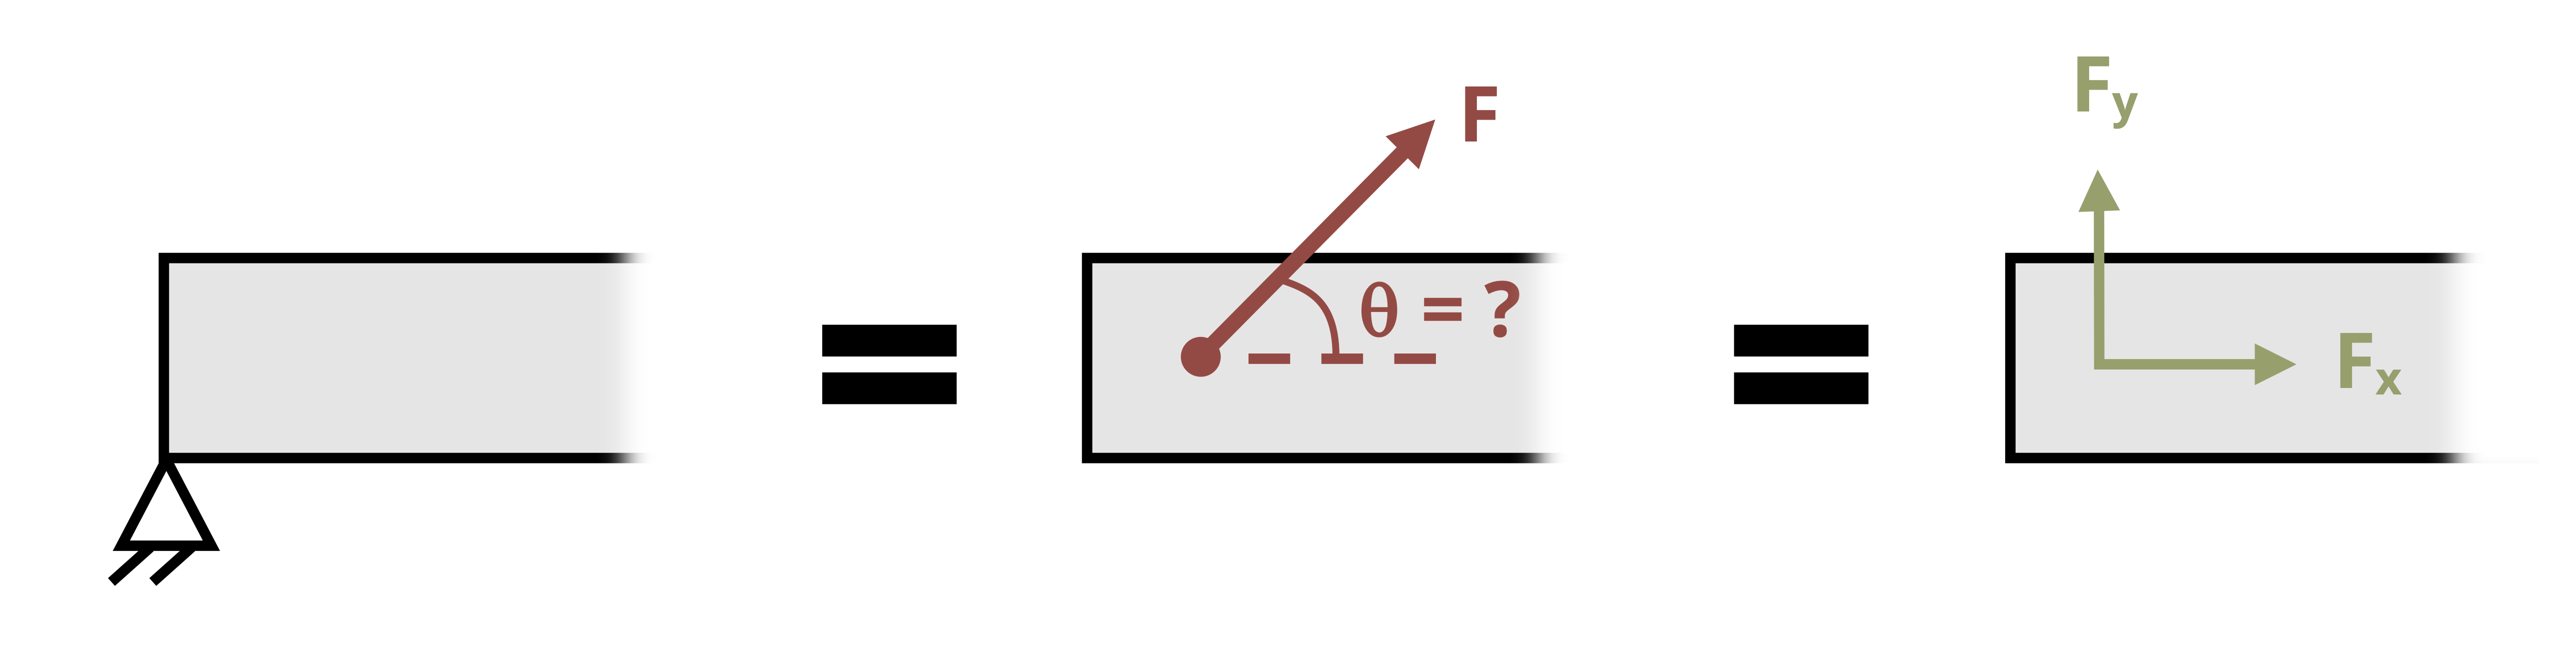
\includegraphics[width=93.75in,height=\textheight]{images/CH1 PNGs/table 1.1 part 1.png} \\
Normal supports

(including rollers, rockers, and smooth contact surface) & Force in the
direction normal to the support. Since the direction is known (normal to
the support), show as total force in the known direction. &
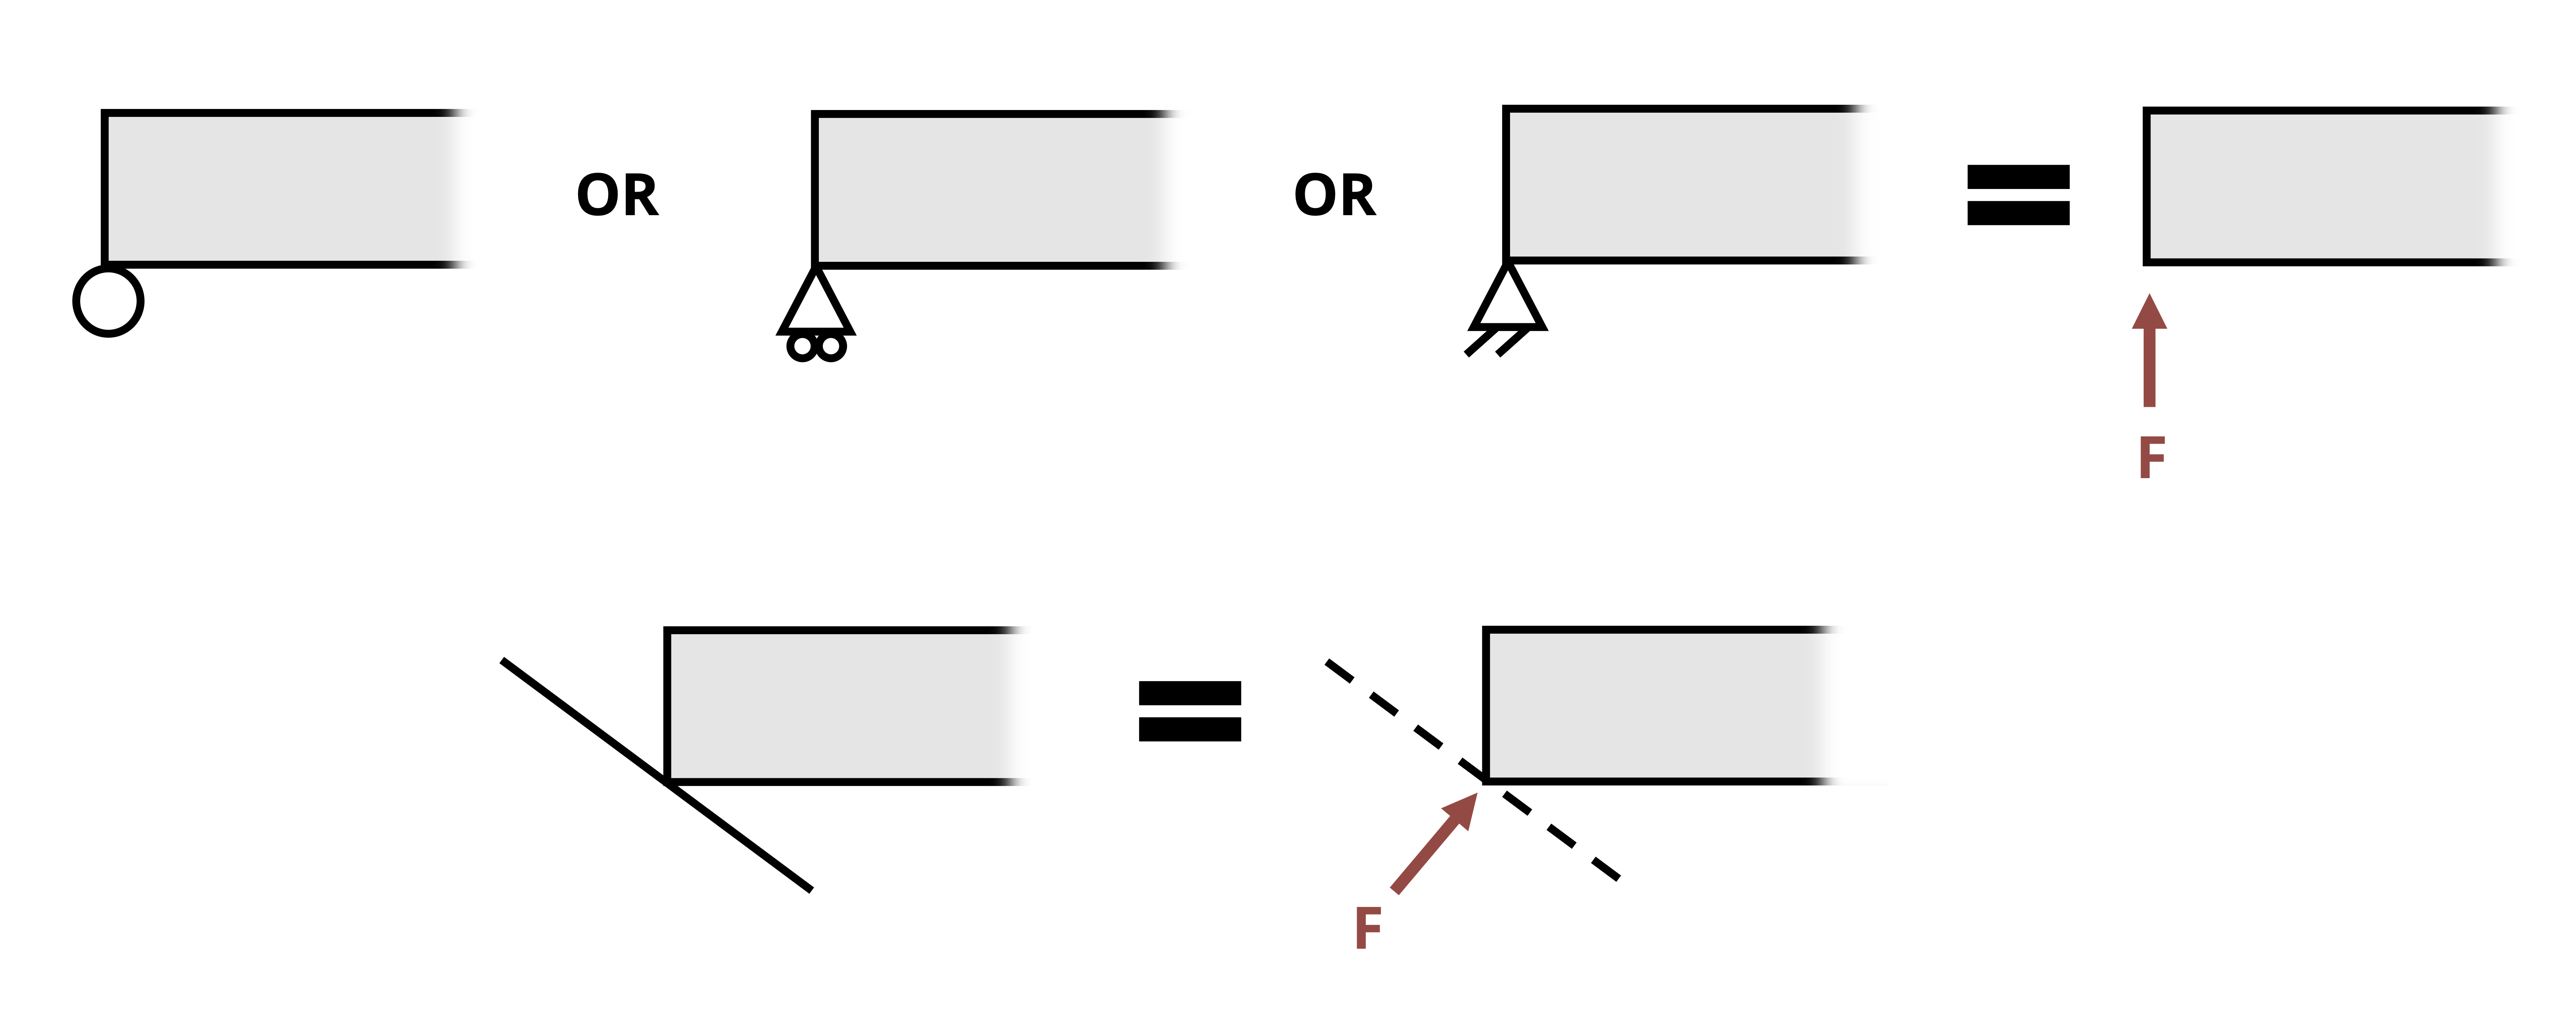
\includegraphics[width=93.75in,height=\textheight]{images/CH1 PNGs/table 1.1 part 2.png} \\
Cables & Force in the direction of the cable. Should always be drawn in
tension. &
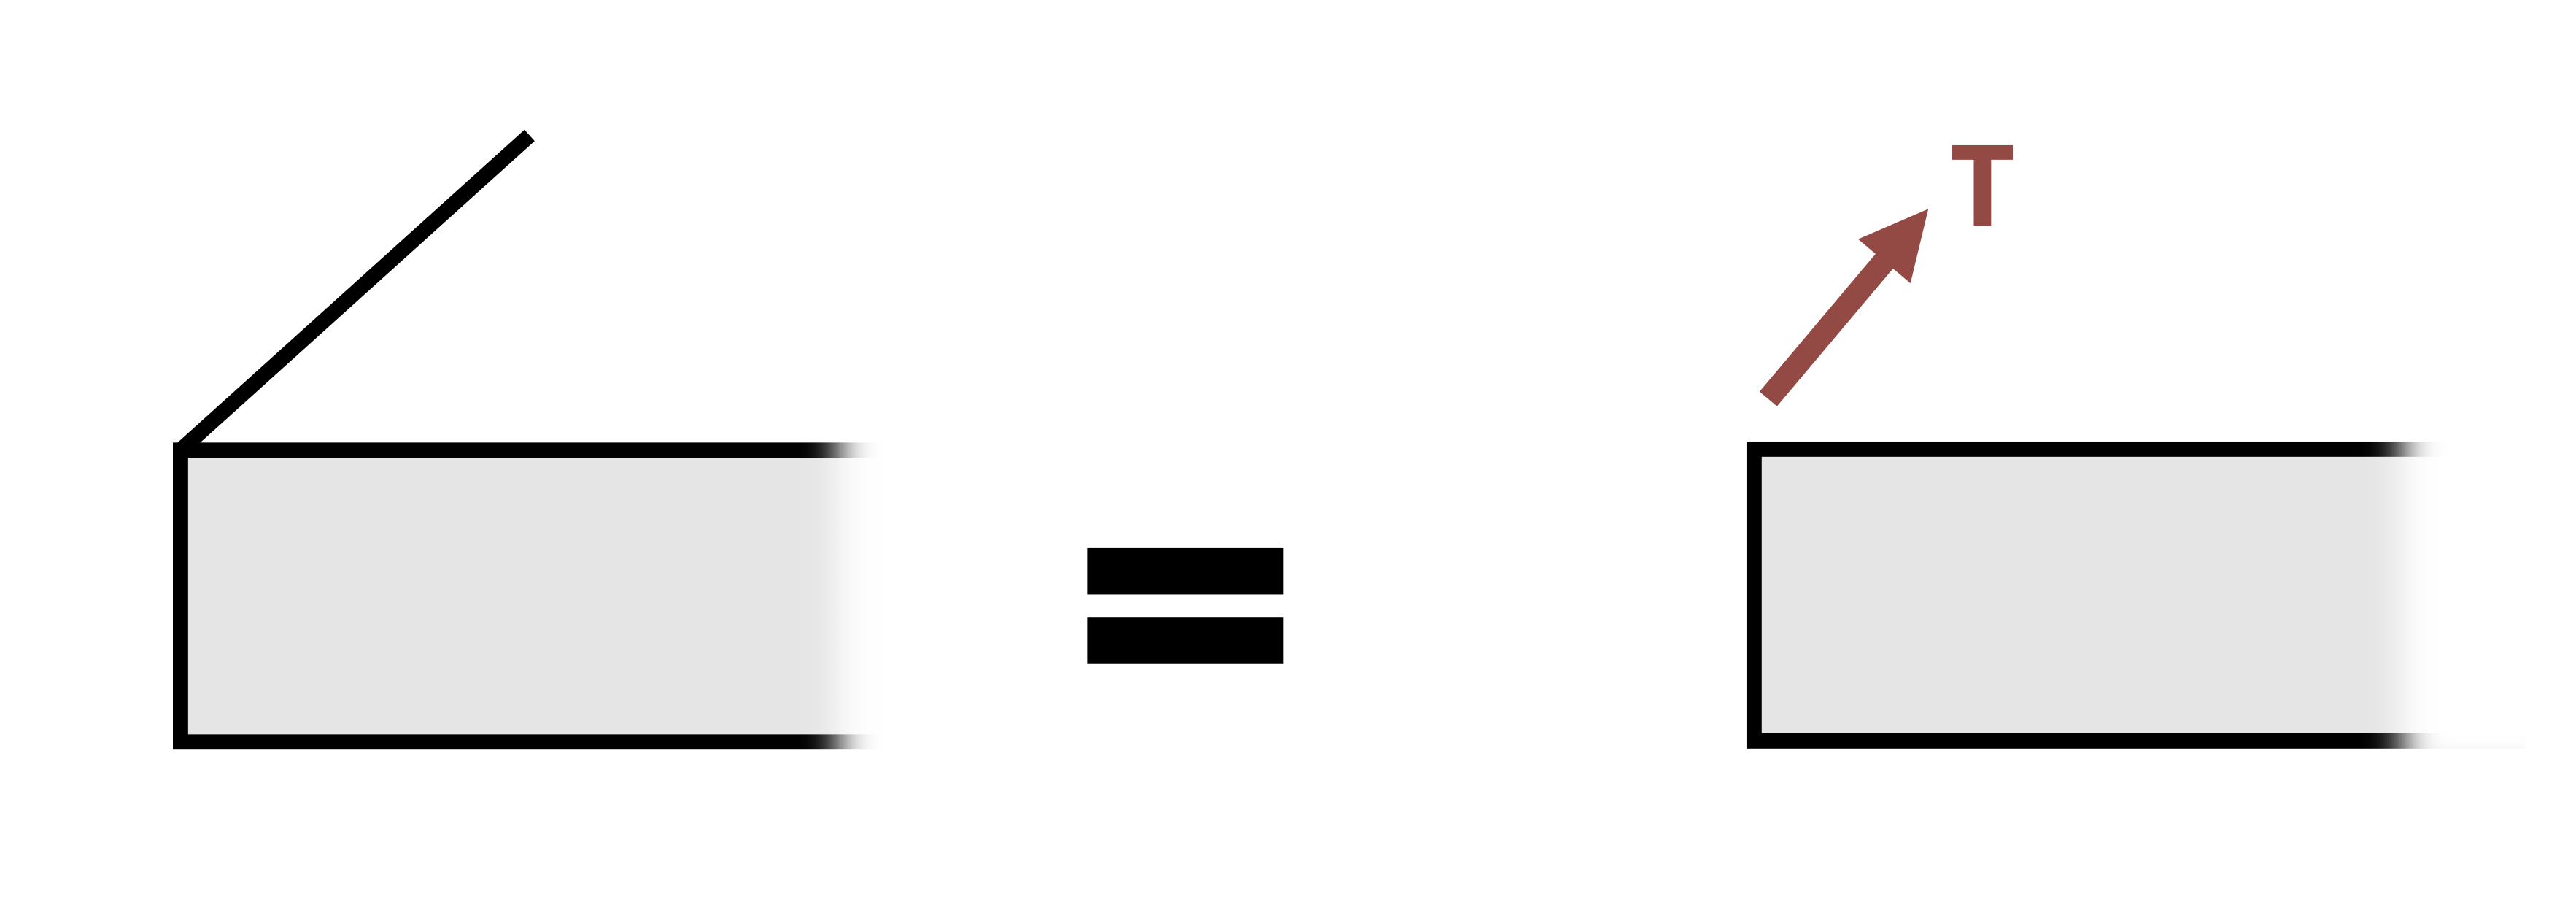
\includegraphics[width=93.75in,height=\textheight]{images/CH1 PNGs/table 1.1 part 3.png} \\
Fixed support & Force in an unknown direction (so draw x and y
components of force) as well as reaction couple moment &
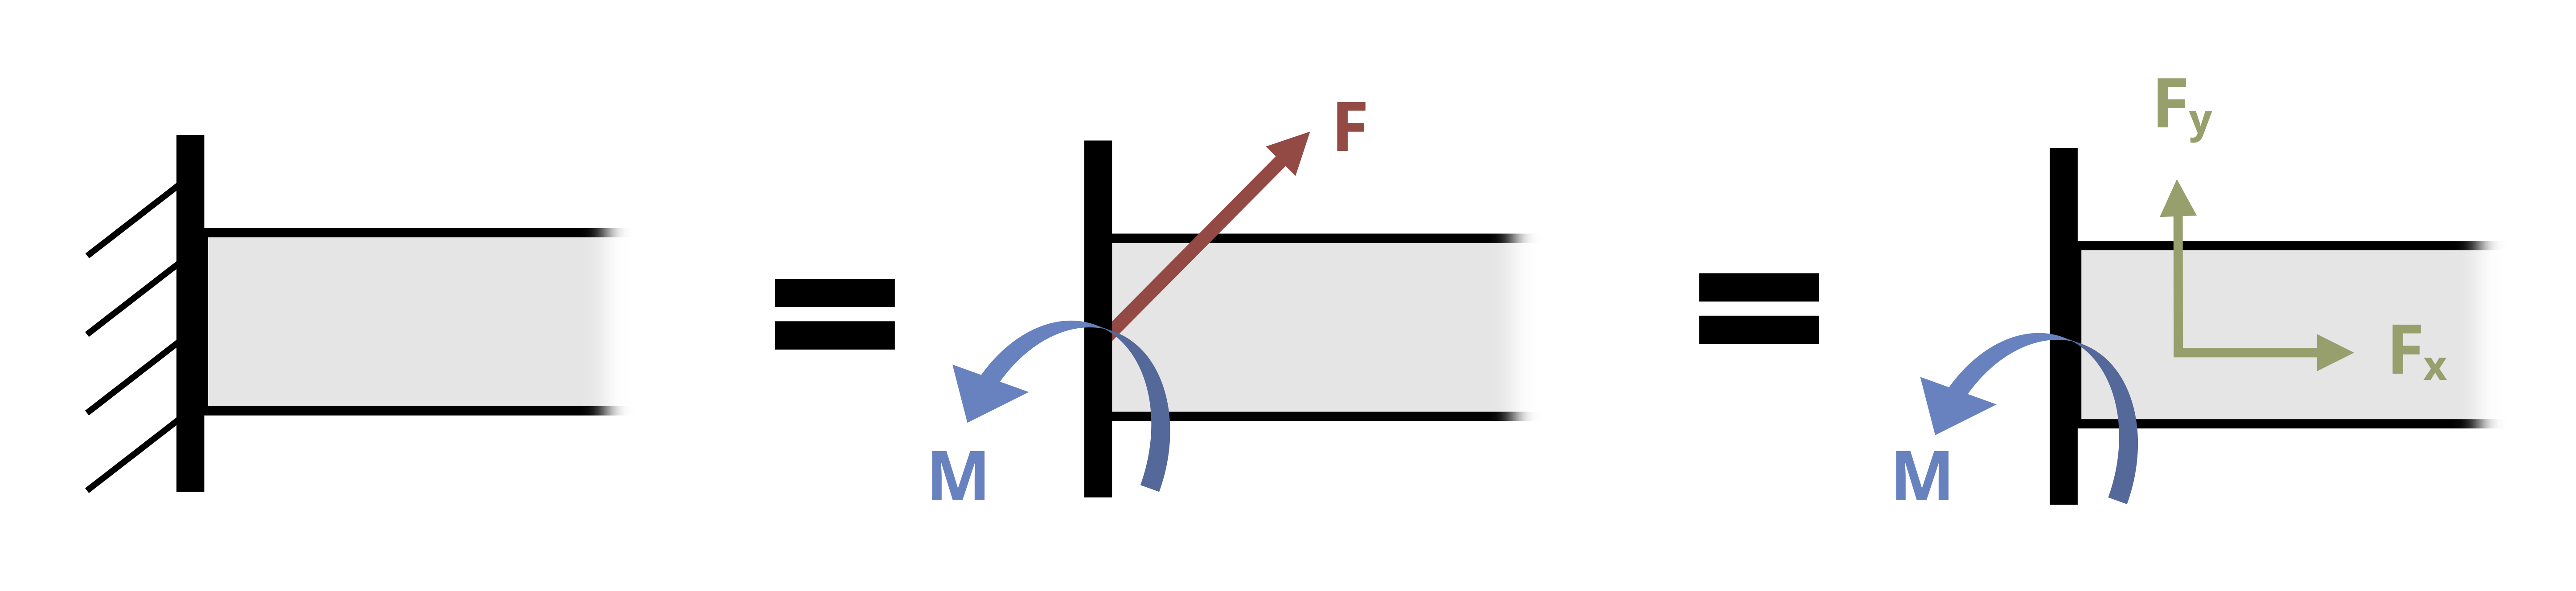
\includegraphics[width=93.75in,height=\textheight]{images/CH1 PNGs/table 1.1 part 4.png} \\
\end{longtable}

Notice that while pins and fixed supports react with a force in a
specific direction, both the magnitude and direction of the force are
unknown until equilibrium equations are applied to solve for them.
Instead of expressing the components of the unknown F in terms of the
unknown θ, the reactions are normally shown as the components
F\textsubscript{x} and F\textsubscript{y}. Once they are found, the
overall magnitude of the force in the pin and its direction can be
calculated
\(\left(F=\sqrt{F_x^2+F_y^2}, \tan \theta_x=\frac{F_y}{F_x}\right)\).

\section{Equilibrium in Two
Dimensions}\label{equilibrium-in-two-dimensions}

Click to expand

Once the FBD is drawn, the next step is to apply the equilibrium
equations. In two dimensions (x-y plane), these are:

\[
\sum F_x=0 \quad \sum F_y=0 \quad \sum M_{\text {any point }}=0
\]

Since there are three equations, a statically determinate problem should
have no more than 3 unknowns.

Example 1.1 illustrates the process of finding external reactions.

\begin{tcolorbox}[enhanced jigsaw, colback=white, colframe=quarto-callout-note-color-frame, leftrule=.75mm, opacitybacktitle=0.6, colbacktitle=quarto-callout-note-color!10!white, arc=.35mm, bottomrule=.15mm, breakable, title=\textcolor{quarto-callout-note-color}{\faInfo}\hspace{0.5em}{Example 1.1}, left=2mm, titlerule=0mm, toptitle=1mm, toprule=.15mm, opacityback=0, rightrule=.15mm, coltitle=black, bottomtitle=1mm]

A 3 ft beam is supported by a pin connection at the wall at point A and
a cable at point C as shown. A load is applied 2 ft away from point A.
Find the force in pin A as well as the tensile force in the cable.

\begin{center}
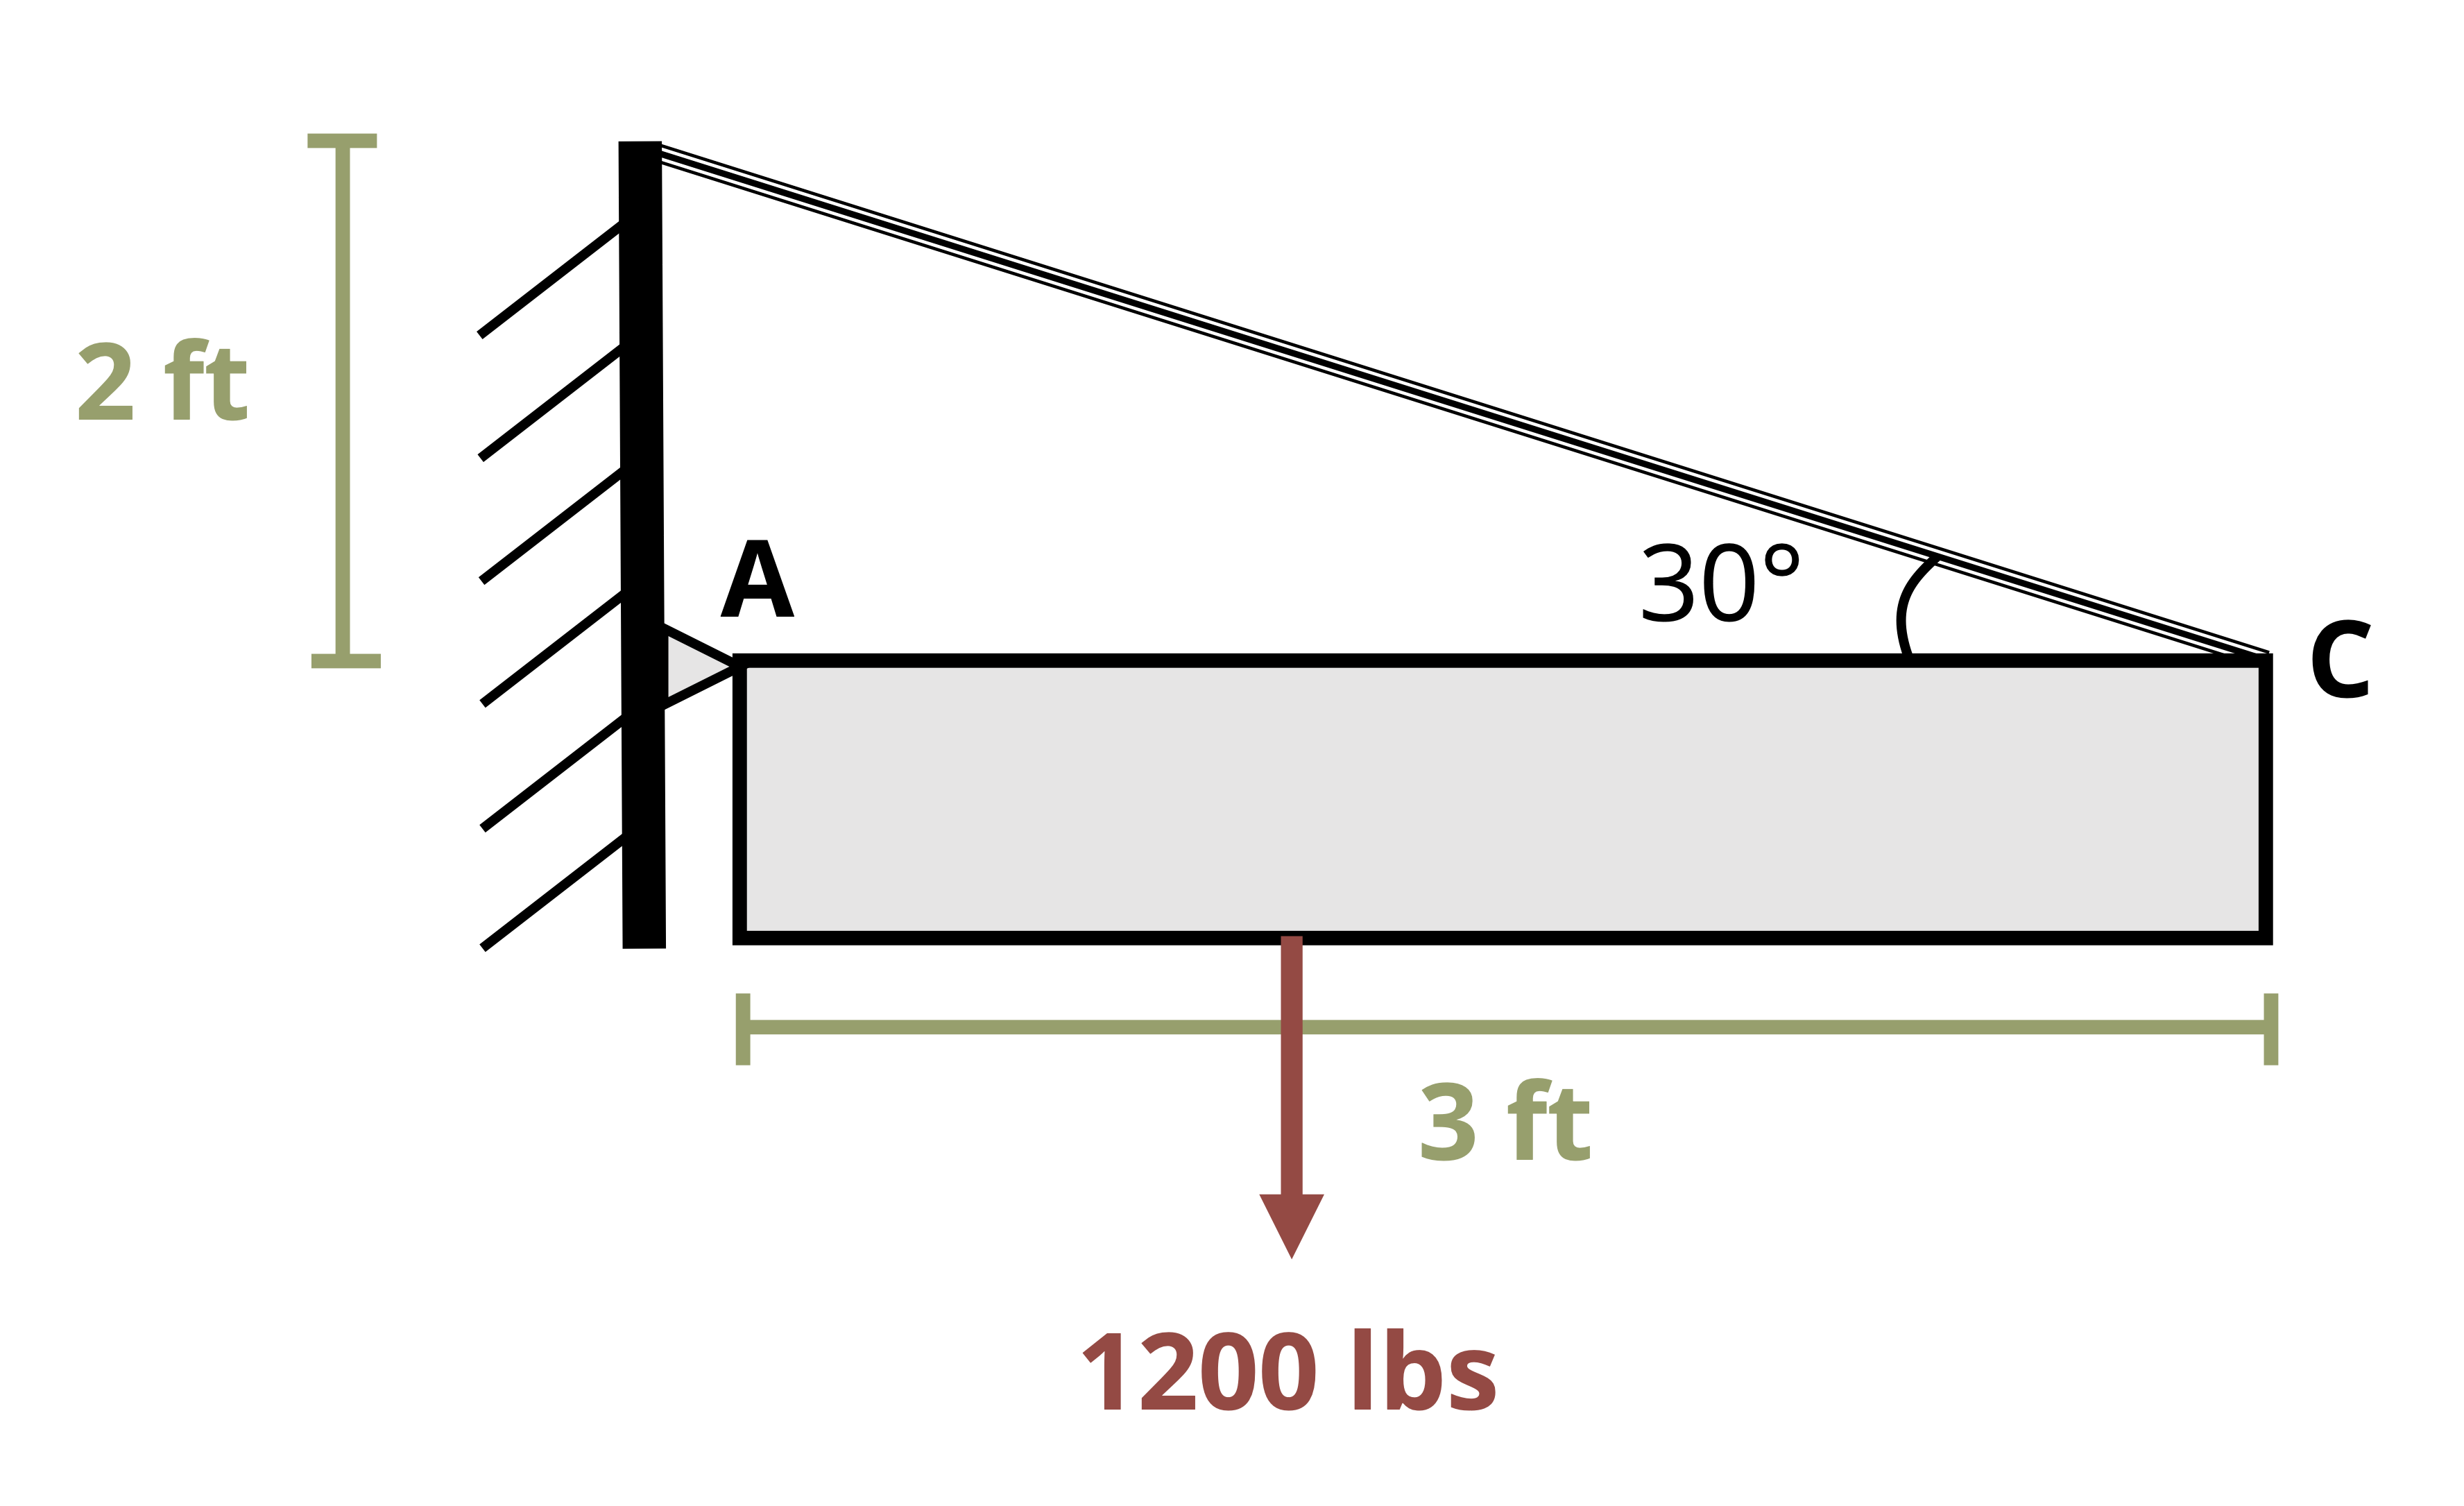
\includegraphics[width=2.75in,height=\textheight]{images/CH1 PNGs/example 1.1 part 1.png}
\end{center}

\textbf{Step 1: Draw the FBD}

Note that a guess needs to be made for the positive or negative sense of
A\textsubscript{x} and A\textsubscript{y}, but the tensile force from a
cable should always be shown to pull away from the body. The correct
sense of A\textsubscript{x} and A\textsubscript{y} will be determined by
obtaining positive or negative answers for the values. A positive answer
means the direction was correctly assumed and a negative answer means
the force should be in the opposite direction.

\begin{center}
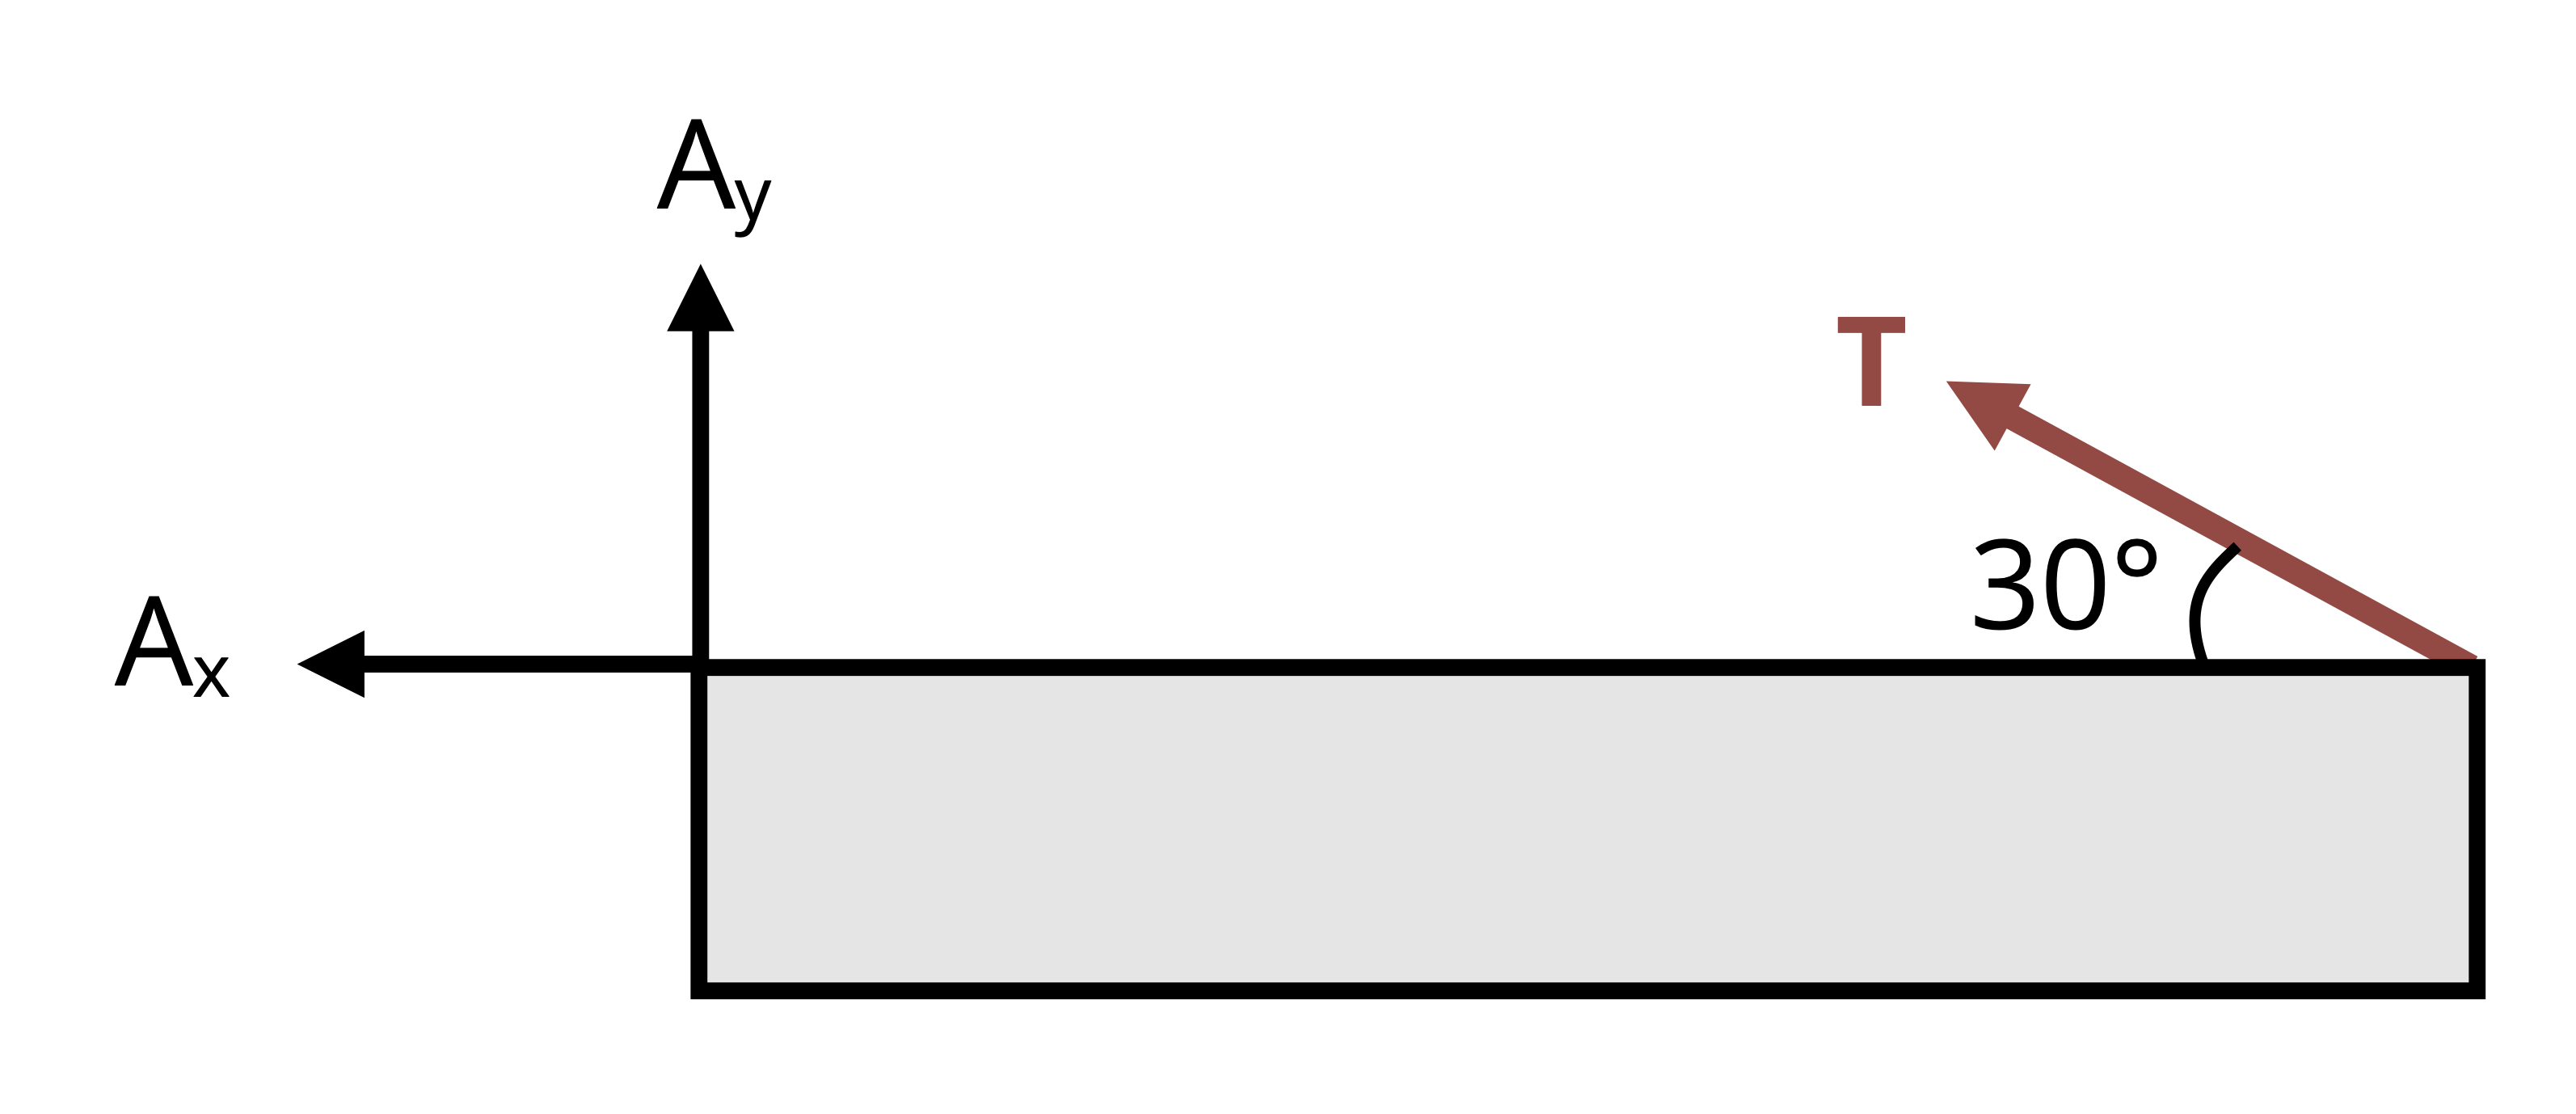
\includegraphics[width=2.64583in,height=\textheight]{images/CH1 PNGs/example 1.1 part 2.png}
\end{center}

\textbf{Step 2: Apply equilibrium equations}

Starting with the moment about A will eliminate two unknowns from the
equation so that tensile force T can be solved for. Then substitute the
result from T into the other two equations to find A\textsubscript{x}
and A\textsubscript{y}.

\[
\begin{aligned}
& \sum M_A=T \sin (30) * 3 ft-1200\text{ lbs }(2 ft)=0 \rightarrow T=1600 \text{ lbs} \\
& \sum F_x=-A_x-T \cos (30)=0 \rightarrow-1384.6 \text{ lbs} \\
& \sum F_y=A_y+T \sin (30)-1200 \text{ lbs}=0 \rightarrow 400 \text{ lbs}
\end{aligned}
\]

Since a negative answer was obtained for A\textsubscript{x}, that force
actually acts in the positive x direction.

The total force in pin A is then
\(F_A=\sqrt{A_x^2+A_y^2}=1441 \text{ lbs}\)

\textbf{Answer: T = 1600 lbs, FA = 1441 lbs}

\end{tcolorbox}

\subsection{Two Force Members}\label{two-force-members}

One special type of pin connection for which the direction of the
reaction force is known is one in which the pin is connected to a
\textbf{two-force member}. Contrary to the name, a two-force member is
not necessarily a member on which only two forces are applied, but
rather it is a member on which forces are applied at only two locations.
A two-force member can be any shape, as is demonstrated in Figure 1.1.
One easy way to recognize a two-force member is to note the presence of
only two connection points (such as two pins) but no other locations at
which a force or moment couple is applied. Once a member is recognized
to be a two-force member, it can be concluded that the resultant force
at both connection points will be equal in magnitude (so
F\textsubscript{A} = F\textsubscript{B} in Figure 1.1) and opposite in
direction and follow a line of action that goes through the connections.
For a straight member, it can also be concluded that the force within
the two-force member (internal reaction as will be discussed in Section
1.1) is equal to the reaction force in the pin.

\begin{figure}[H]

{\centering 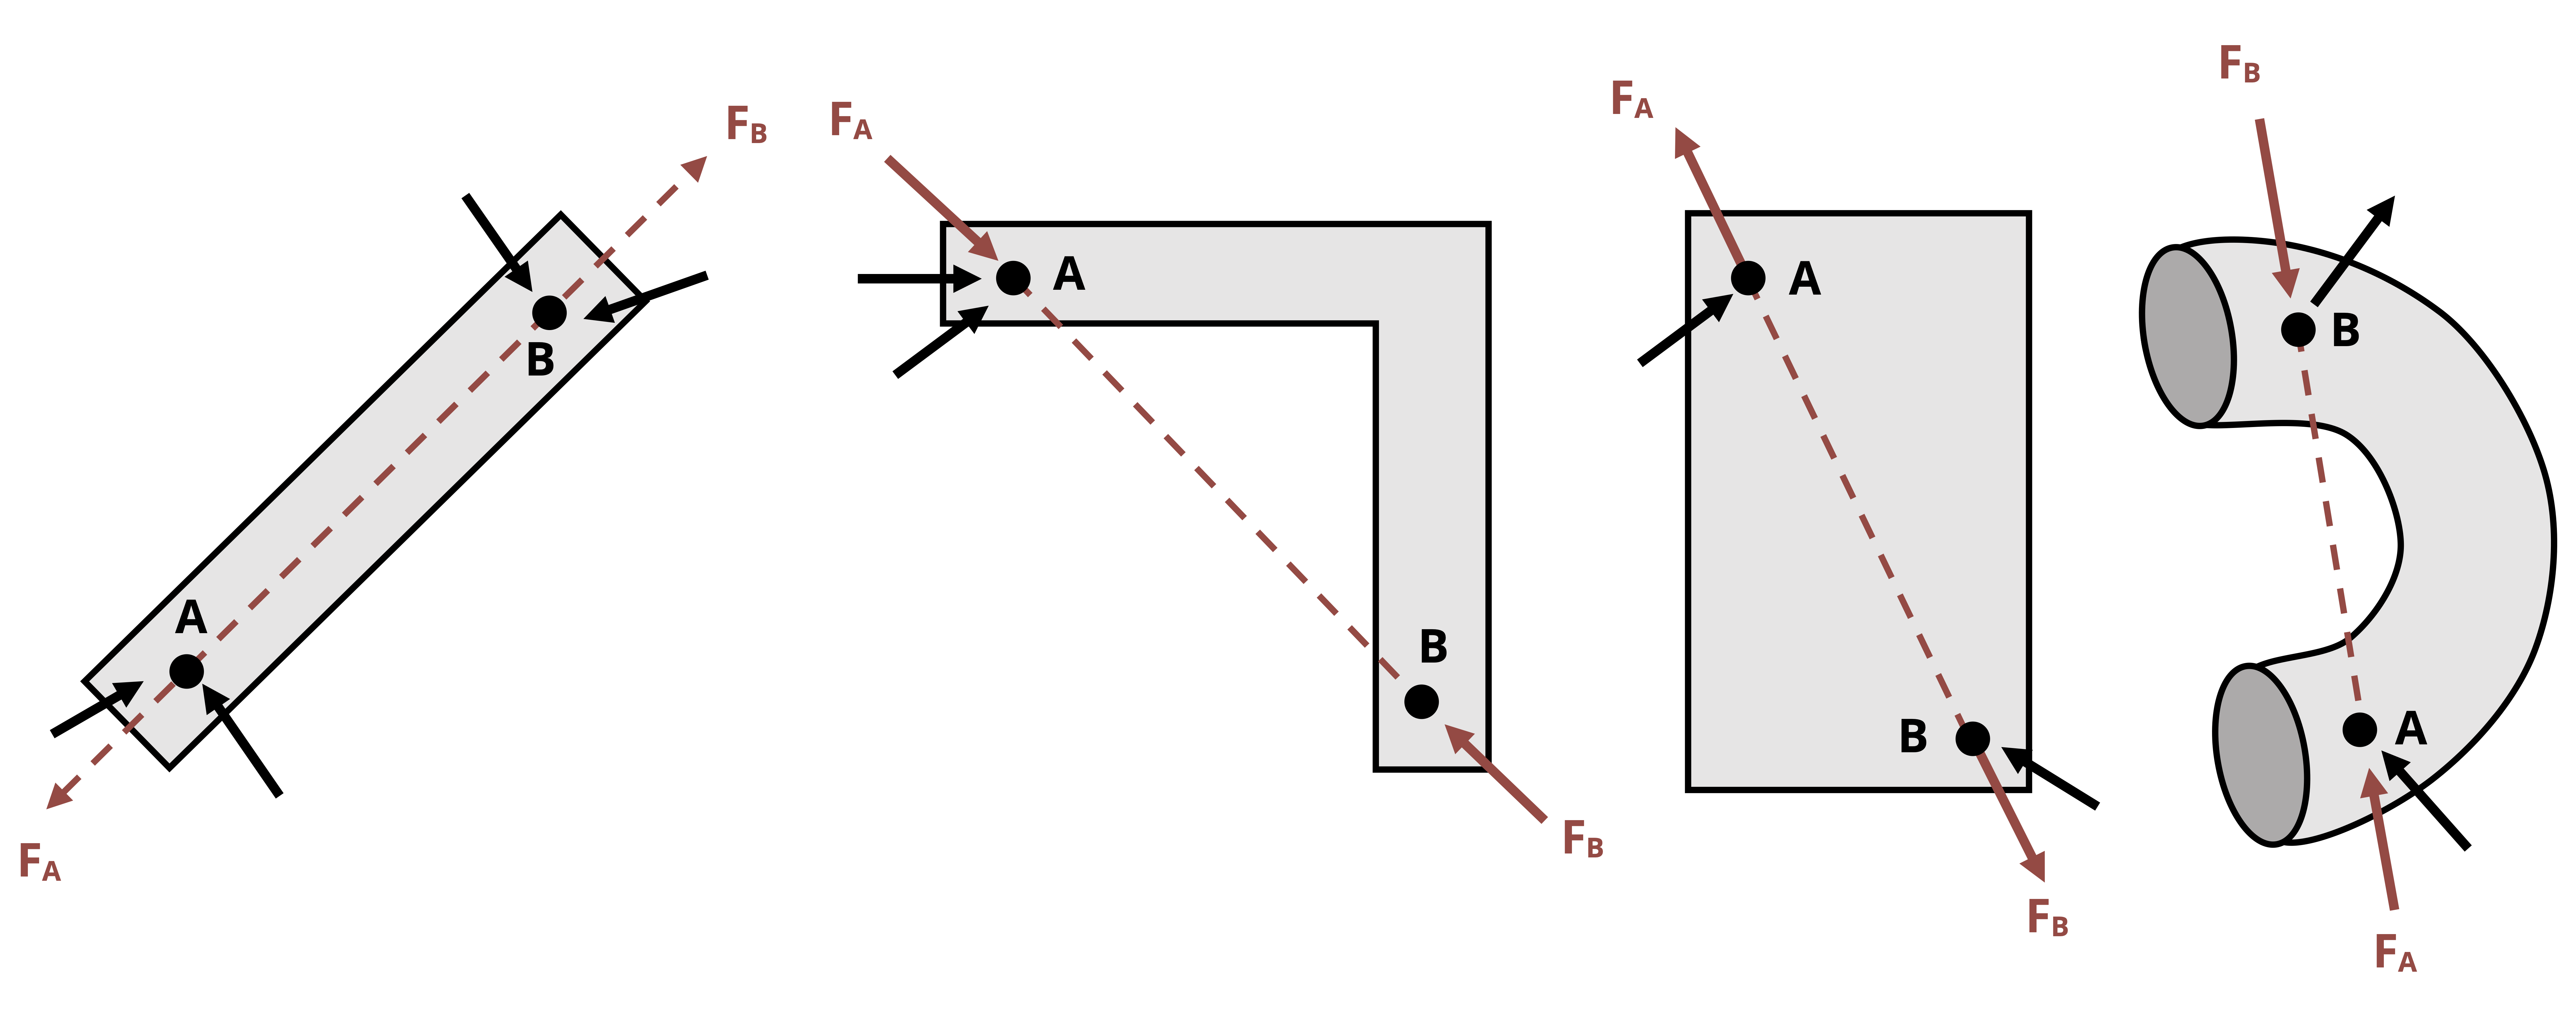
\includegraphics[width=6.6875in,height=\textheight]{images/CH1 PNGs/figure 1.1.png}

}

\caption{Figure 1.1: Illustrations of two force members showing the line
of action of the reaction force passing through the joints. Note that
F\textsubscript{A} = F\textsubscript{B}.}

\end{figure}%

The presence and recognition of two force members can make some
otherwise statically indeterminate problems become statically
determinate. This is demonstrated in Example 1.2 below.

\begin{tcolorbox}[enhanced jigsaw, colback=white, colframe=quarto-callout-note-color-frame, leftrule=.75mm, opacitybacktitle=0.6, colbacktitle=quarto-callout-note-color!10!white, arc=.35mm, bottomrule=.15mm, breakable, title={Example 1.2}, left=2mm, titlerule=0mm, toptitle=1mm, toprule=.15mm, opacityback=0, rightrule=.15mm, coltitle=black, bottomtitle=1mm]

Determine the force in pin C and in pin A.

\begin{center}
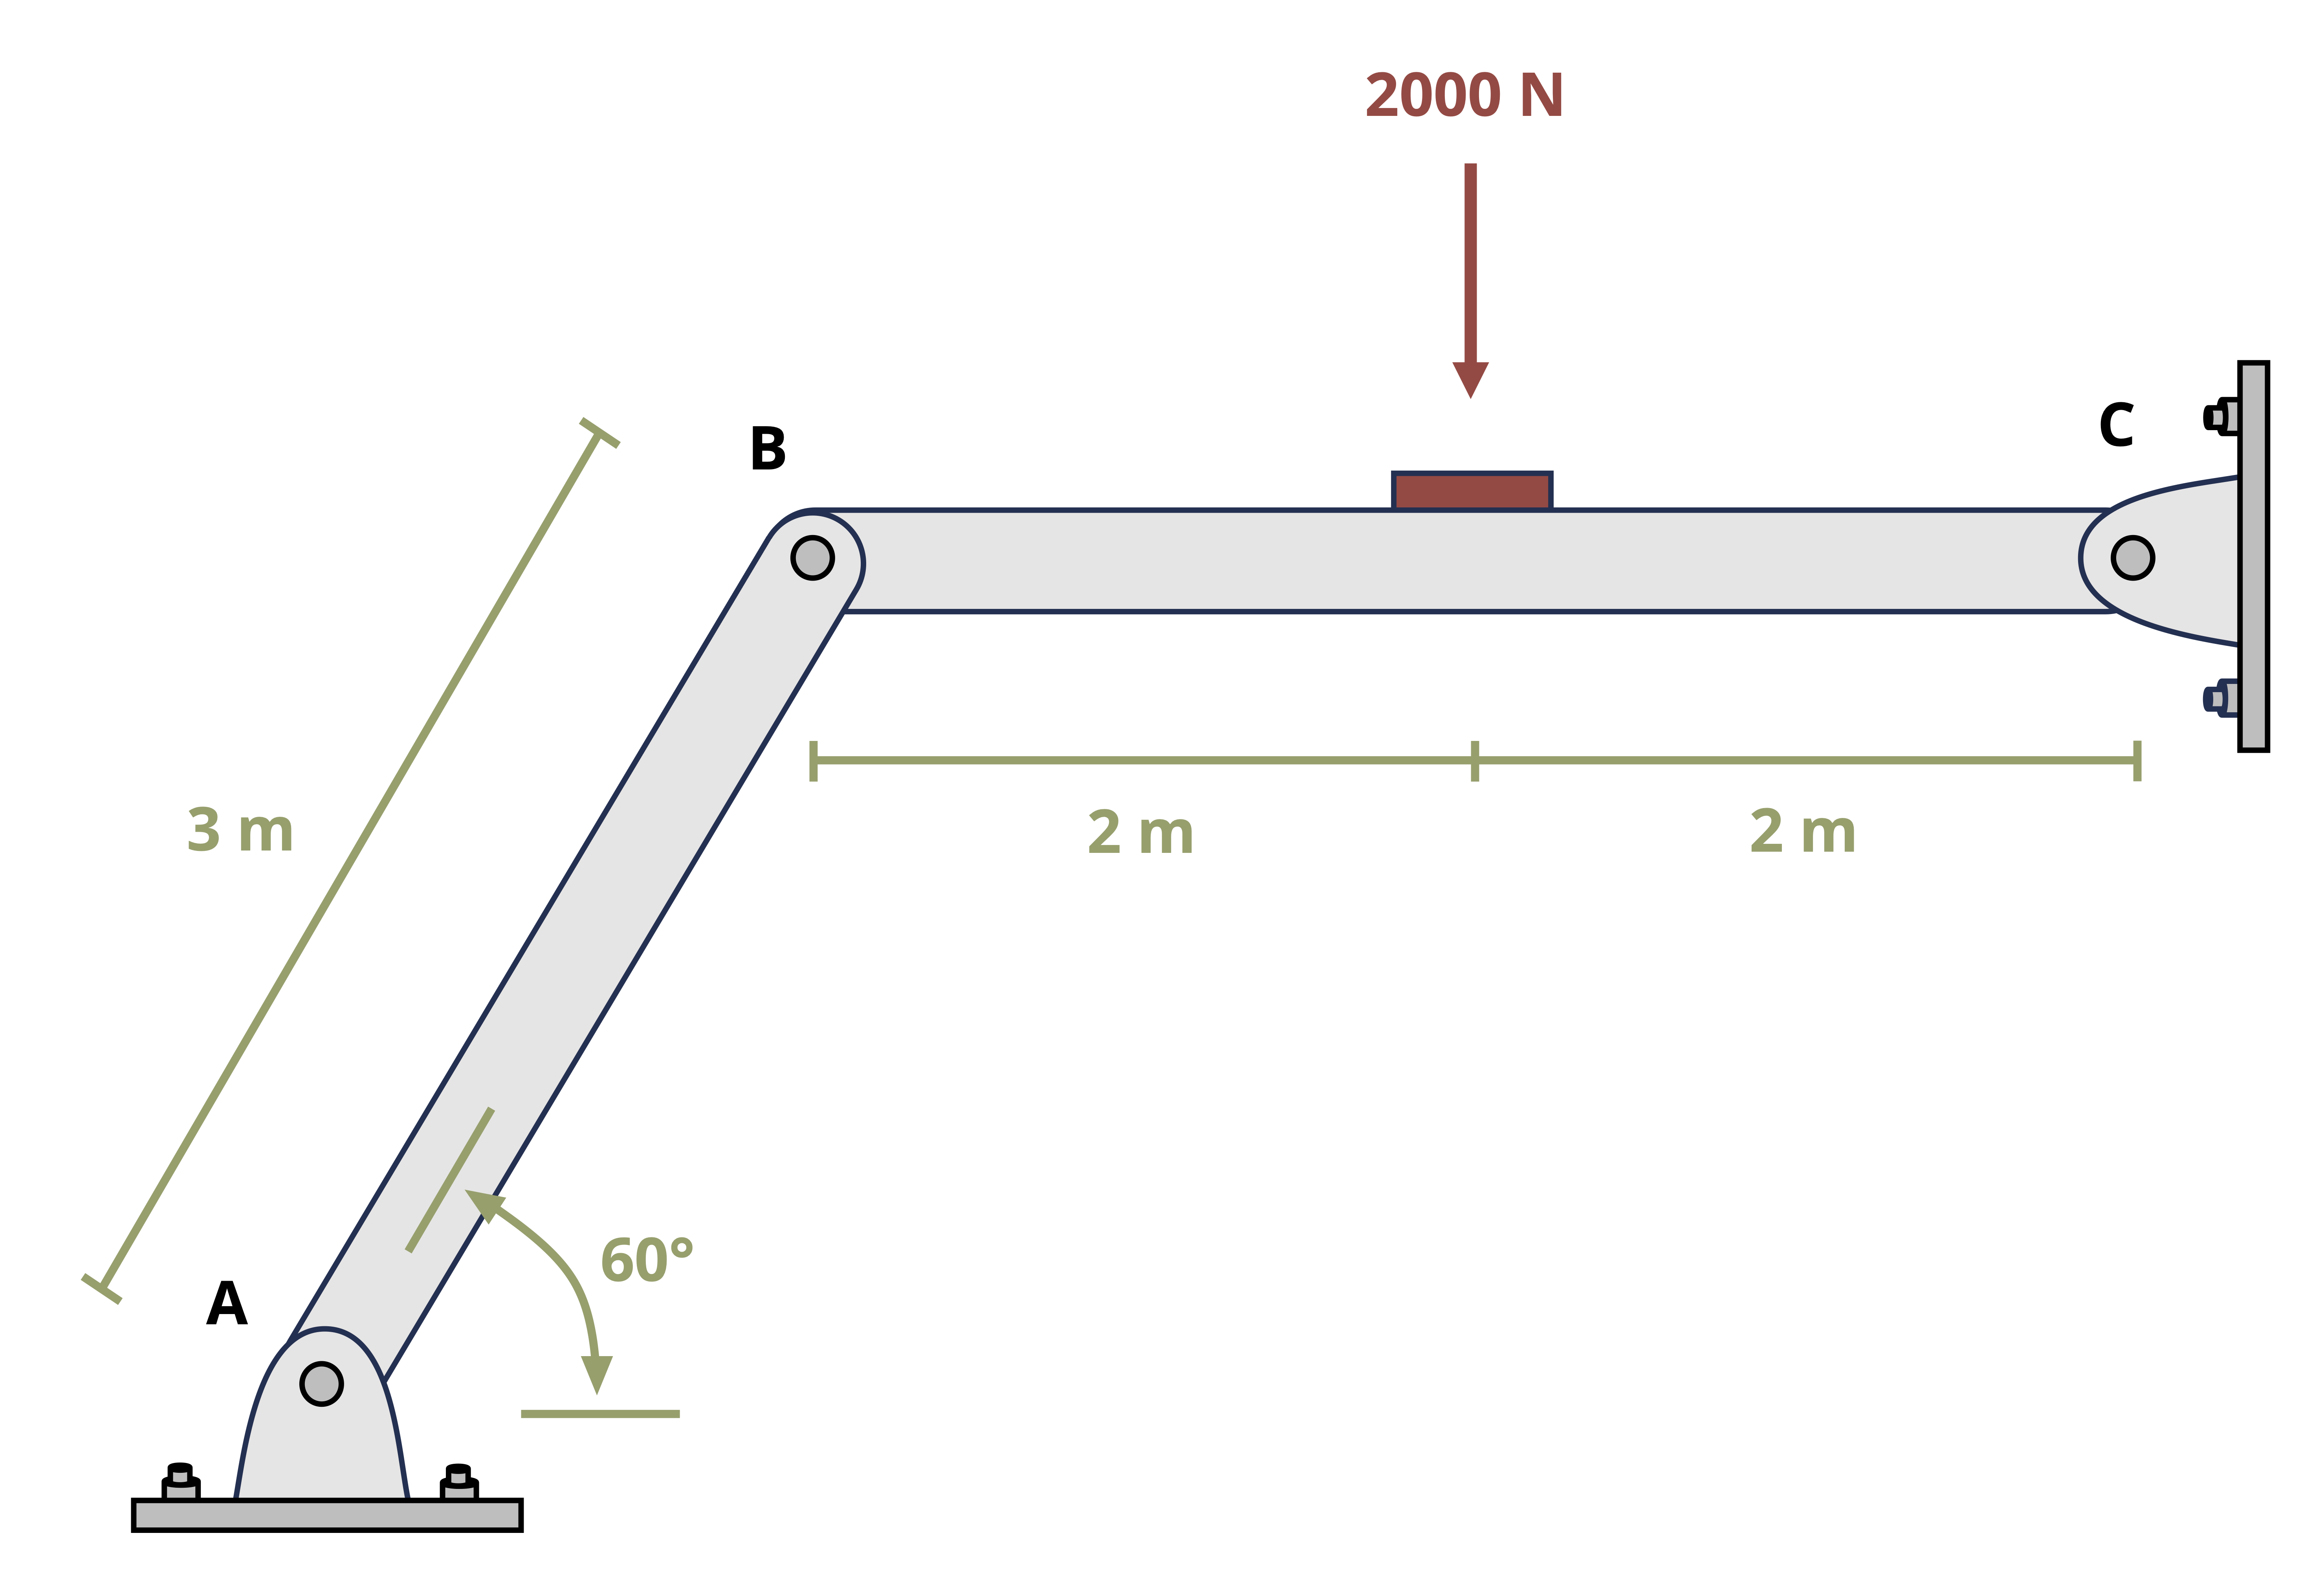
\includegraphics[width=4.61458in,height=\textheight]{images/CH1 PNGs/example 1.2 part 1.png}
\end{center}

\textbf{Step 1: Draw the FBD}

\begin{center}
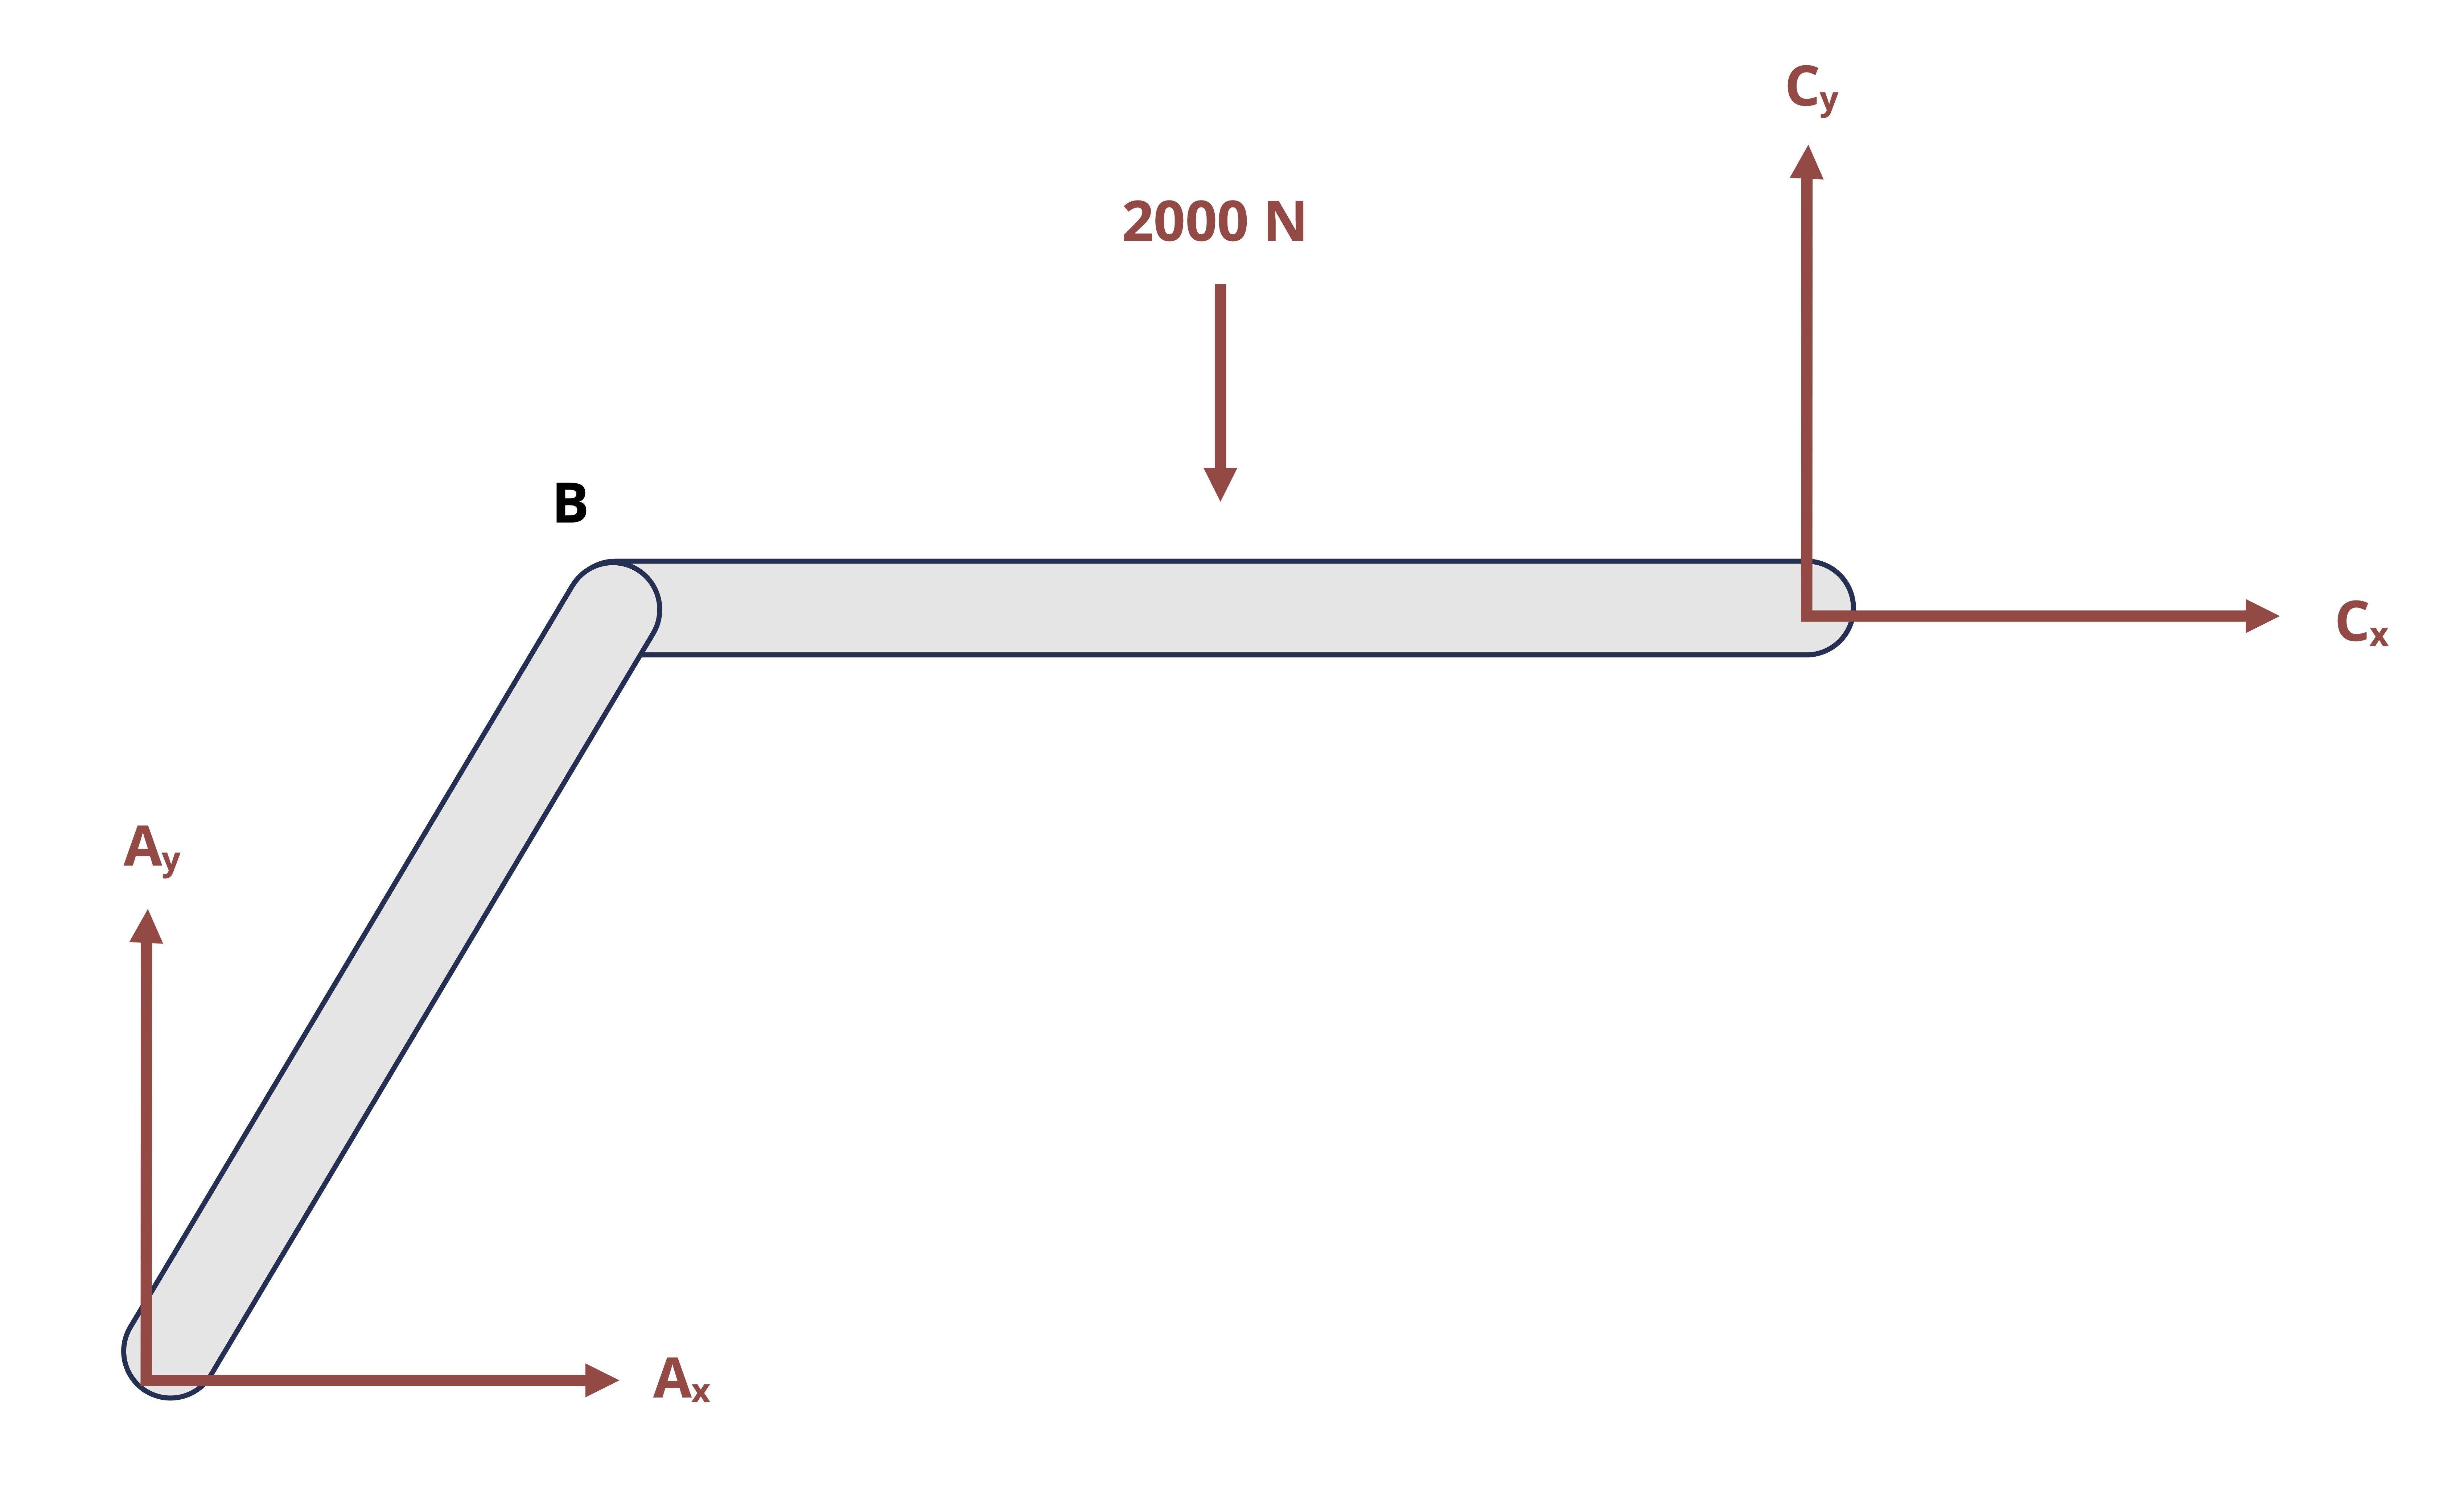
\includegraphics[width=5.10417in,height=\textheight]{images/CH1 PNGs/example 1.2 part 2.png}
\end{center}

Based on this FBD, it appears that there are 4 unknowns and therefore
not solvable by just 3 equilibrium equations. However, recognizing that
bar AB is a two-force member (since there is a pin at A and a pin at B
but no other forces acting on that bar), it can be taken as known that
the line of action of the reaction force at A goes through points A and
B. Thus, the FBD can be redrawn with just 3 unknowns:

\begin{center}
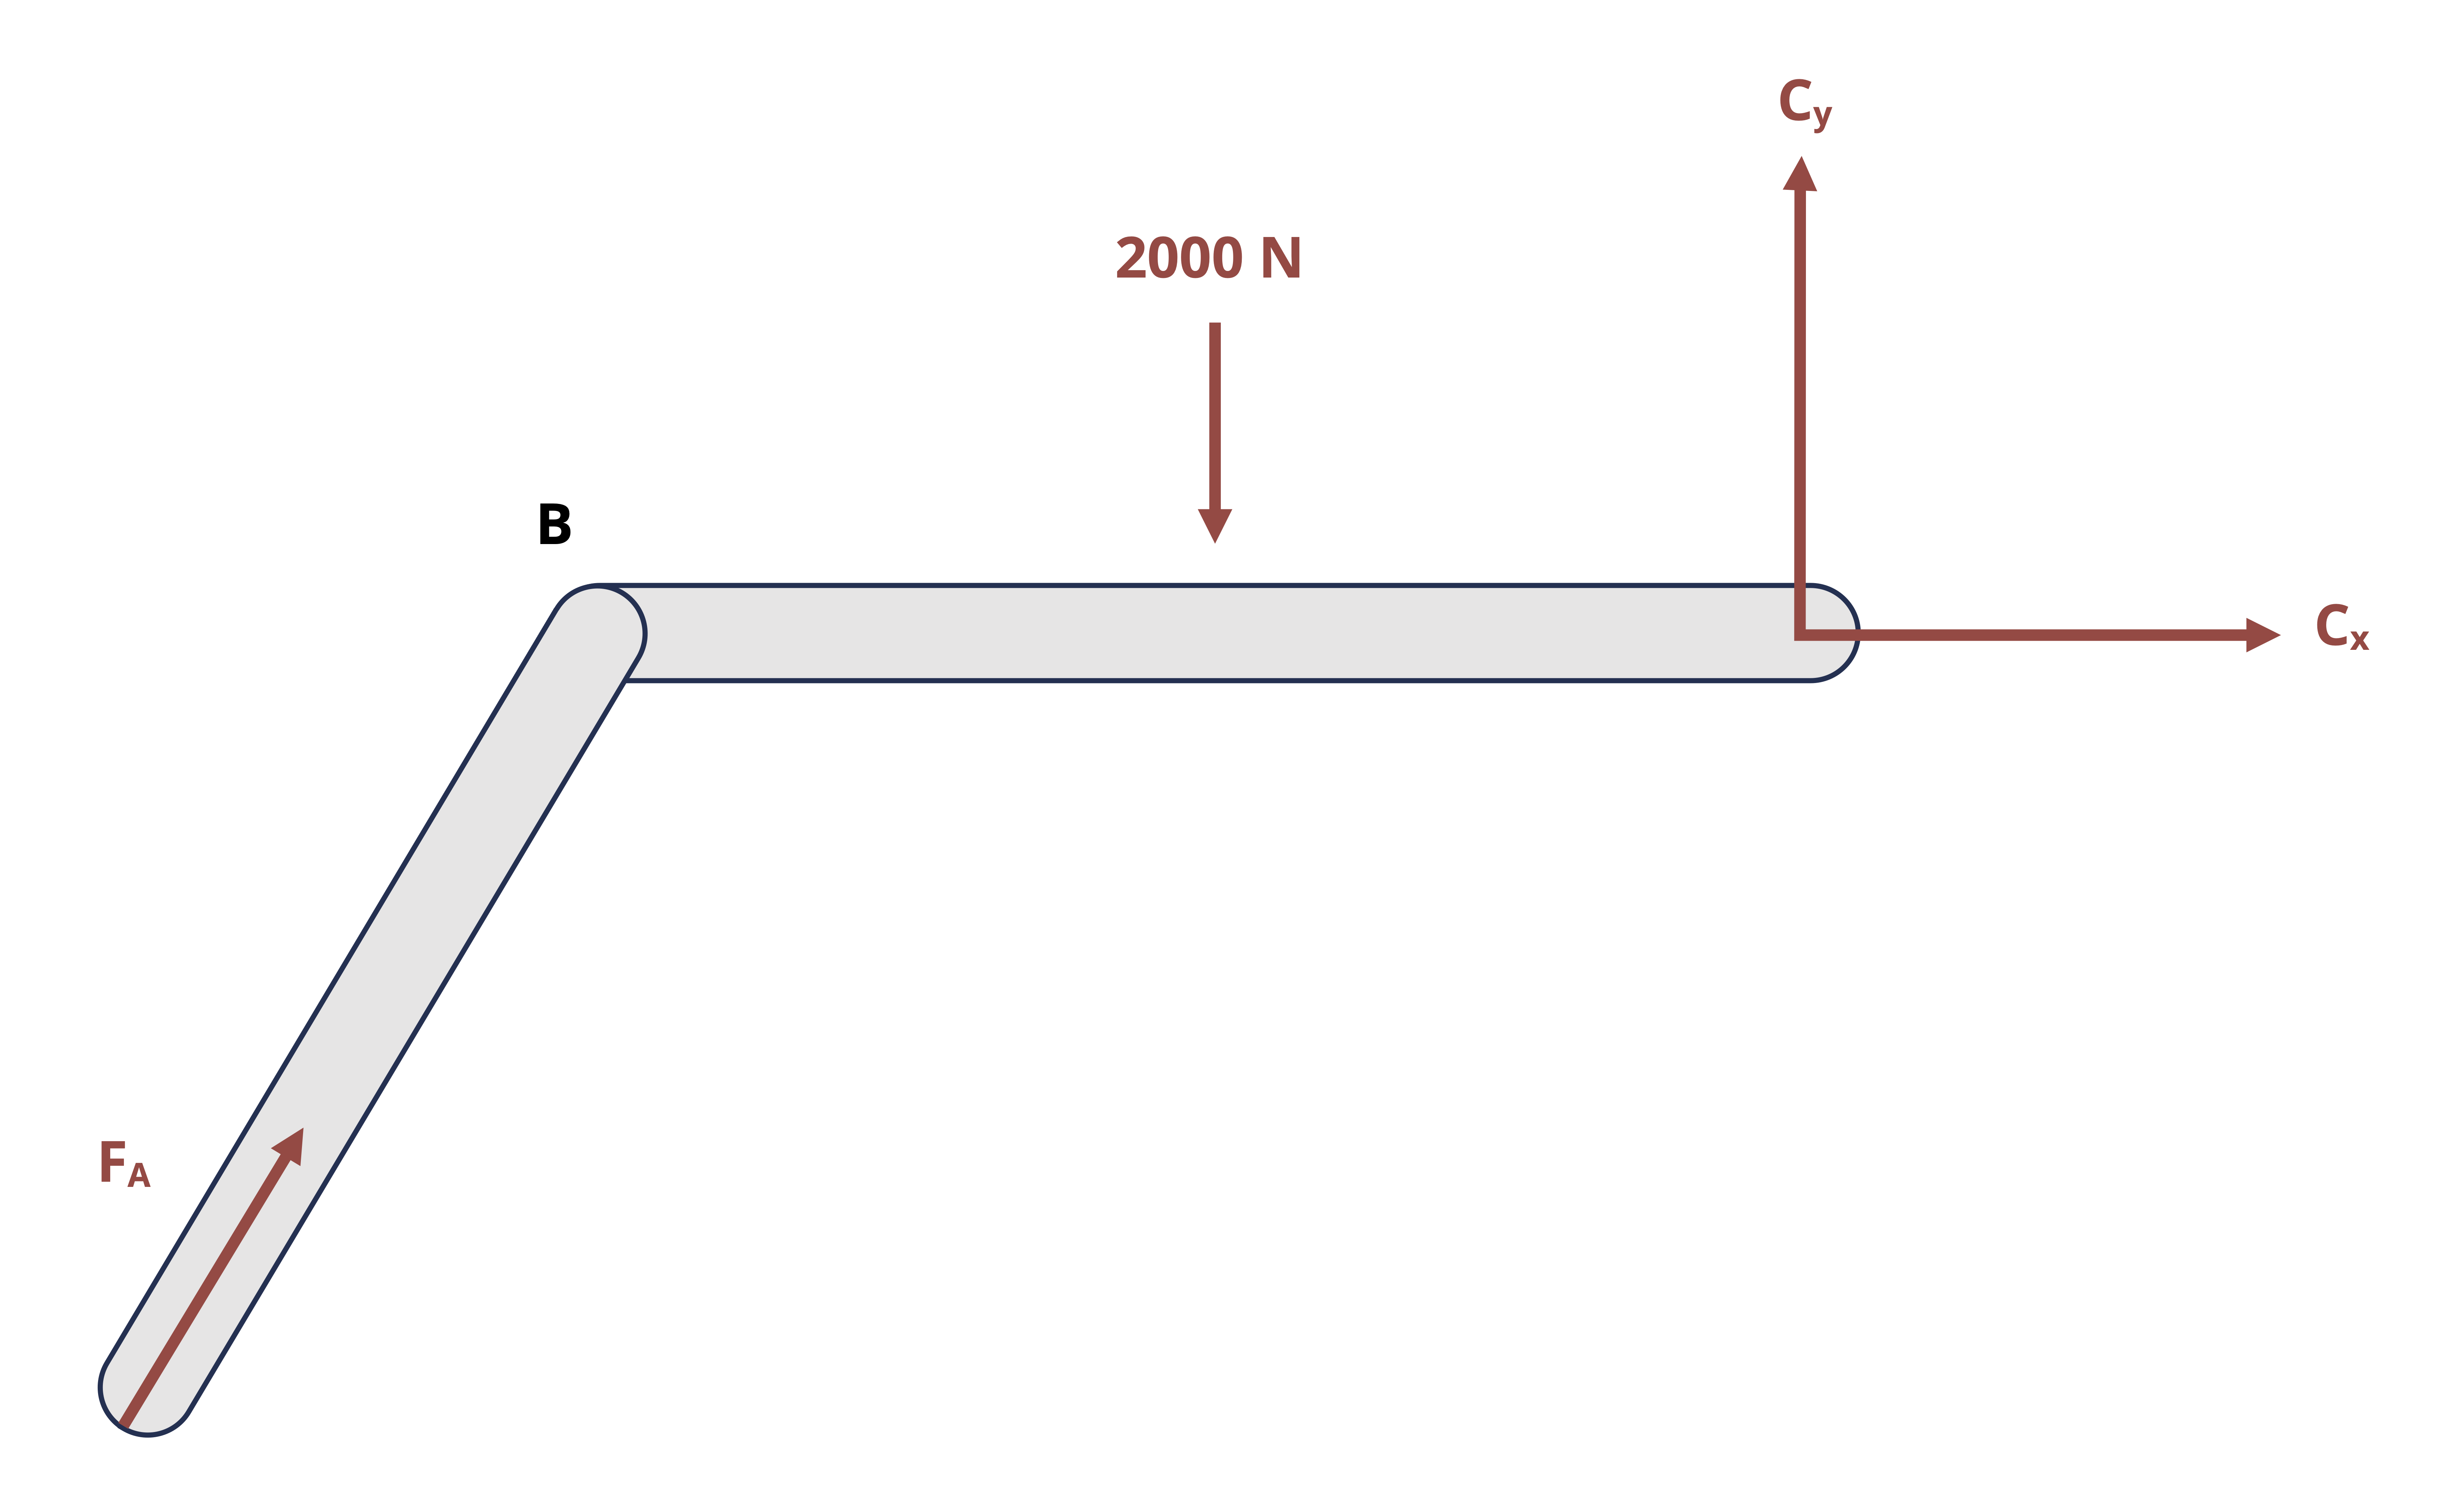
\includegraphics[width=4.83333in,height=\textheight]{images/CH1 PNGs/example 1.2 part 3.png}
\end{center}

\textbf{Step 2: Apply equilibrium equations}

\[
\begin{aligned}
\text{(1)}& \sum M_C=-F_A \cos \left(60^{\circ}\right) \times(3 m) \sin \left(60^{\circ}\right)+F_A \sin \left(60^{\circ}\right) \times\left(4 m+3 m\left(\cos \left(60^{\circ}\right)\right)-2000 \times 2 m=0\right. \\
\text{(2)}& \sum F_x=F_A \cos \left(60^{\circ}\right)+C_x=0 \\
\text{(3)}& \sum F_y=F_A \sin \left(60^{\circ}\right)-2000+C_y=0
\end{aligned}
\]

Solving (1) for F\textsubscript{A} yields F\textsubscript{A} = 1154.7 N

Subbing this result into (1) and (2) yields C\textsubscript{x} = -577.4
N and C\textsubscript{y} = 1000 N

\[
F_C=\sqrt{C_x^2+C_y^2}=1154.7 \mathrm{~N}
\]

\textbf{Answer: F\textsubscript{A} = 1155 N and F\textsubscript{C} =
1155 N}

\end{tcolorbox}

\section{Internal Reactions}\label{internal-reactions}

Click to expand

Internal reactions can refer to forces and moments at connection points
between members (such as a pin connecting multiple members of a frame,
machine, or truss), as well as to reactions at any point in a continuous
body (for example a point in the middle of a beam). These reactions are
the forces and/or moments necessary to hold a structure or a body
together and are ultimately the aspect of loading that is needed to
determine if and how a body will deform or even break.

\subsection{Internal reactions at a connection with two force
members}\label{internal-reactions-at-a-connection-with-two-force-members}

Pins that connect members can be represented on an FBD in the same way
as pins that connect the structure to external supports. That is, the
reaction would be drawn as the two components of the overall force.
However, the connected members would be considered as separate bodies,
as if the connecting pin were pulled out and the members separated. The
pin reactions would then be drawn on the FBD for each separated member.
Since the pin would exert equal and opposite forces on the connected
members, one needs to be careful to show the reaction forces in opposite
directions on the FBD's of those members. All three equilibrium
equations can be applied separately to each member so one could
theoretically solve for 3 times the number of unknowns as separate FBD's
drawn.

However, just as was discussed above, when one of the connected members
is a two-force member, the reaction at the pin will be known to follow a
line of action that goes through the points of application of the forces
on the two-force member. Example 1.3 demonstrates these concepts.

\begin{tcolorbox}[enhanced jigsaw, colback=white, colframe=quarto-callout-note-color-frame, leftrule=.75mm, opacitybacktitle=0.6, colbacktitle=quarto-callout-note-color!10!white, arc=.35mm, bottomrule=.15mm, breakable, title={Example 1.3}, left=2mm, titlerule=0mm, toptitle=1mm, toprule=.15mm, opacityback=0, rightrule=.15mm, coltitle=black, bottomtitle=1mm]

A plant hanger is secured to a wall with a pin and additionally
supported by a brace that is pin connected to the hanger at B and to the
wall at C. Determine the external reactions at A and C as well as the
reaction in the internal pin B.

\begin{center}
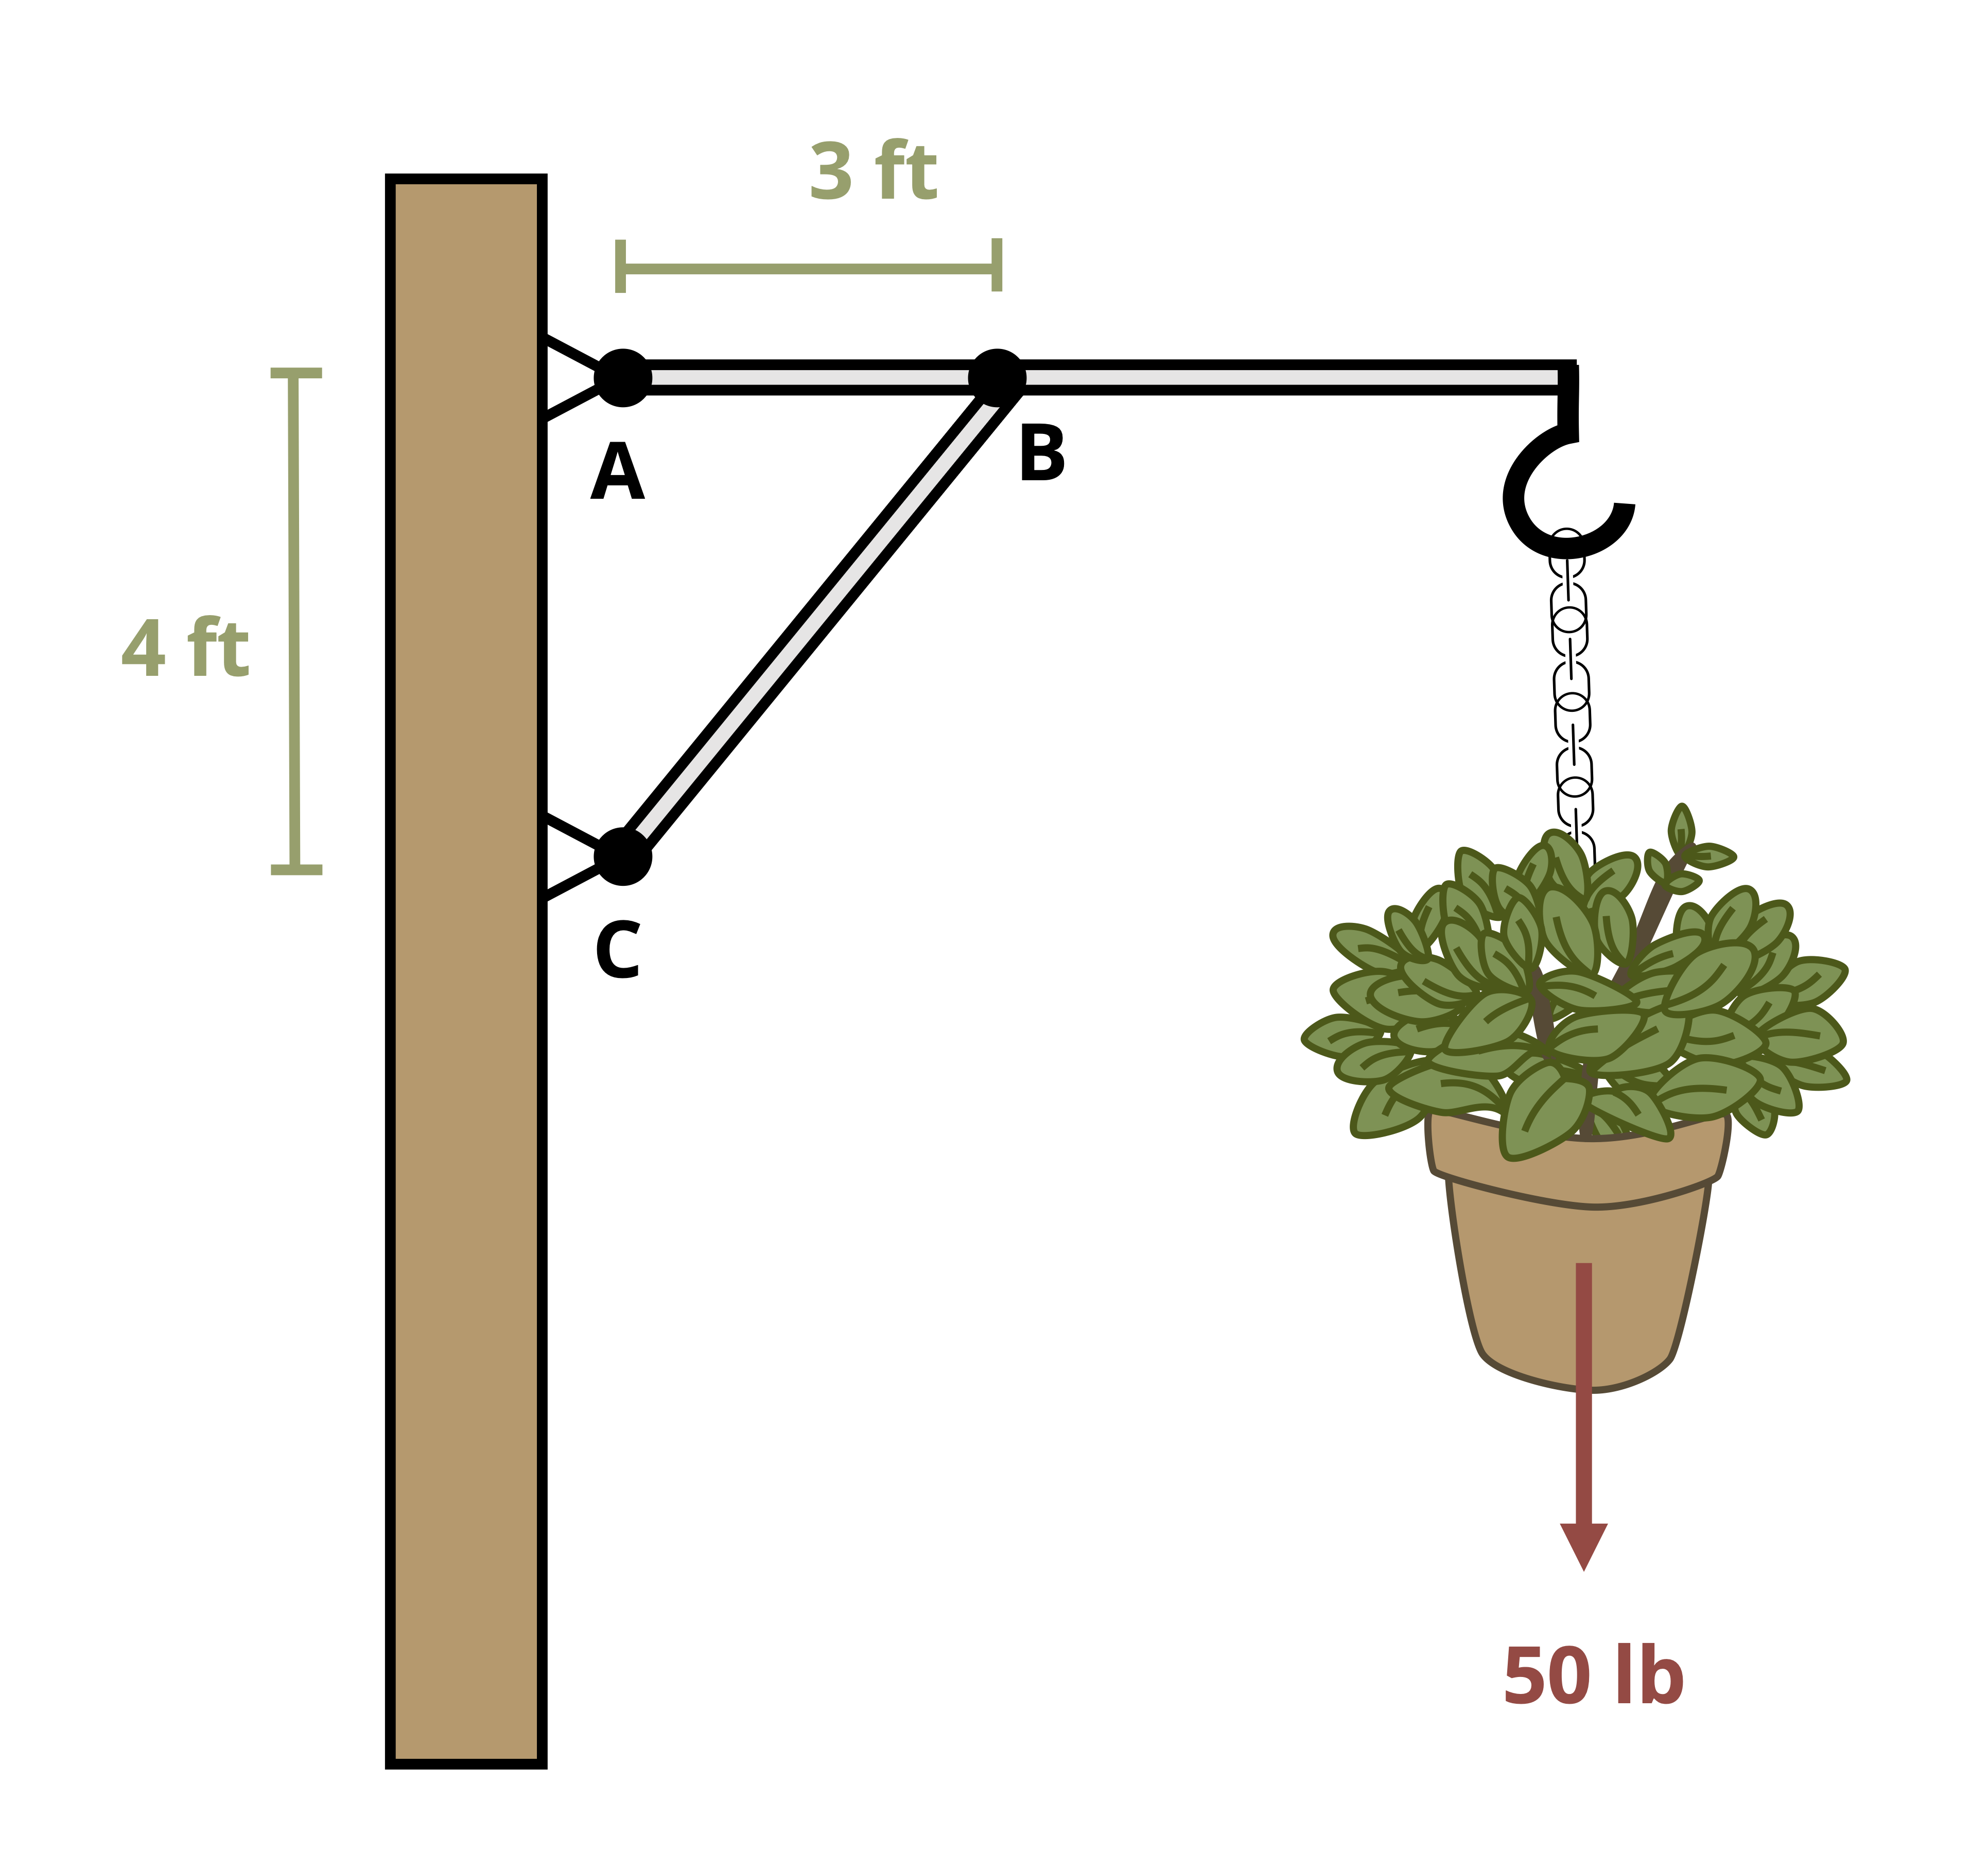
\includegraphics[width=3.28125in,height=\textheight]{images/CH1 PNGs/example 1.3 part 1.png}
\end{center}

If we do not notice that BC is a two-force member, we would approach the
problem by separating the brace from the hanger and drawing an FBD of
each part separately. Notice that B\textsubscript{x} and
B\textsubscript{y} are drawn in opposite directions in the two different
diagrams since the pin will exert an equal and opposite force on each
bar.

\begin{center}
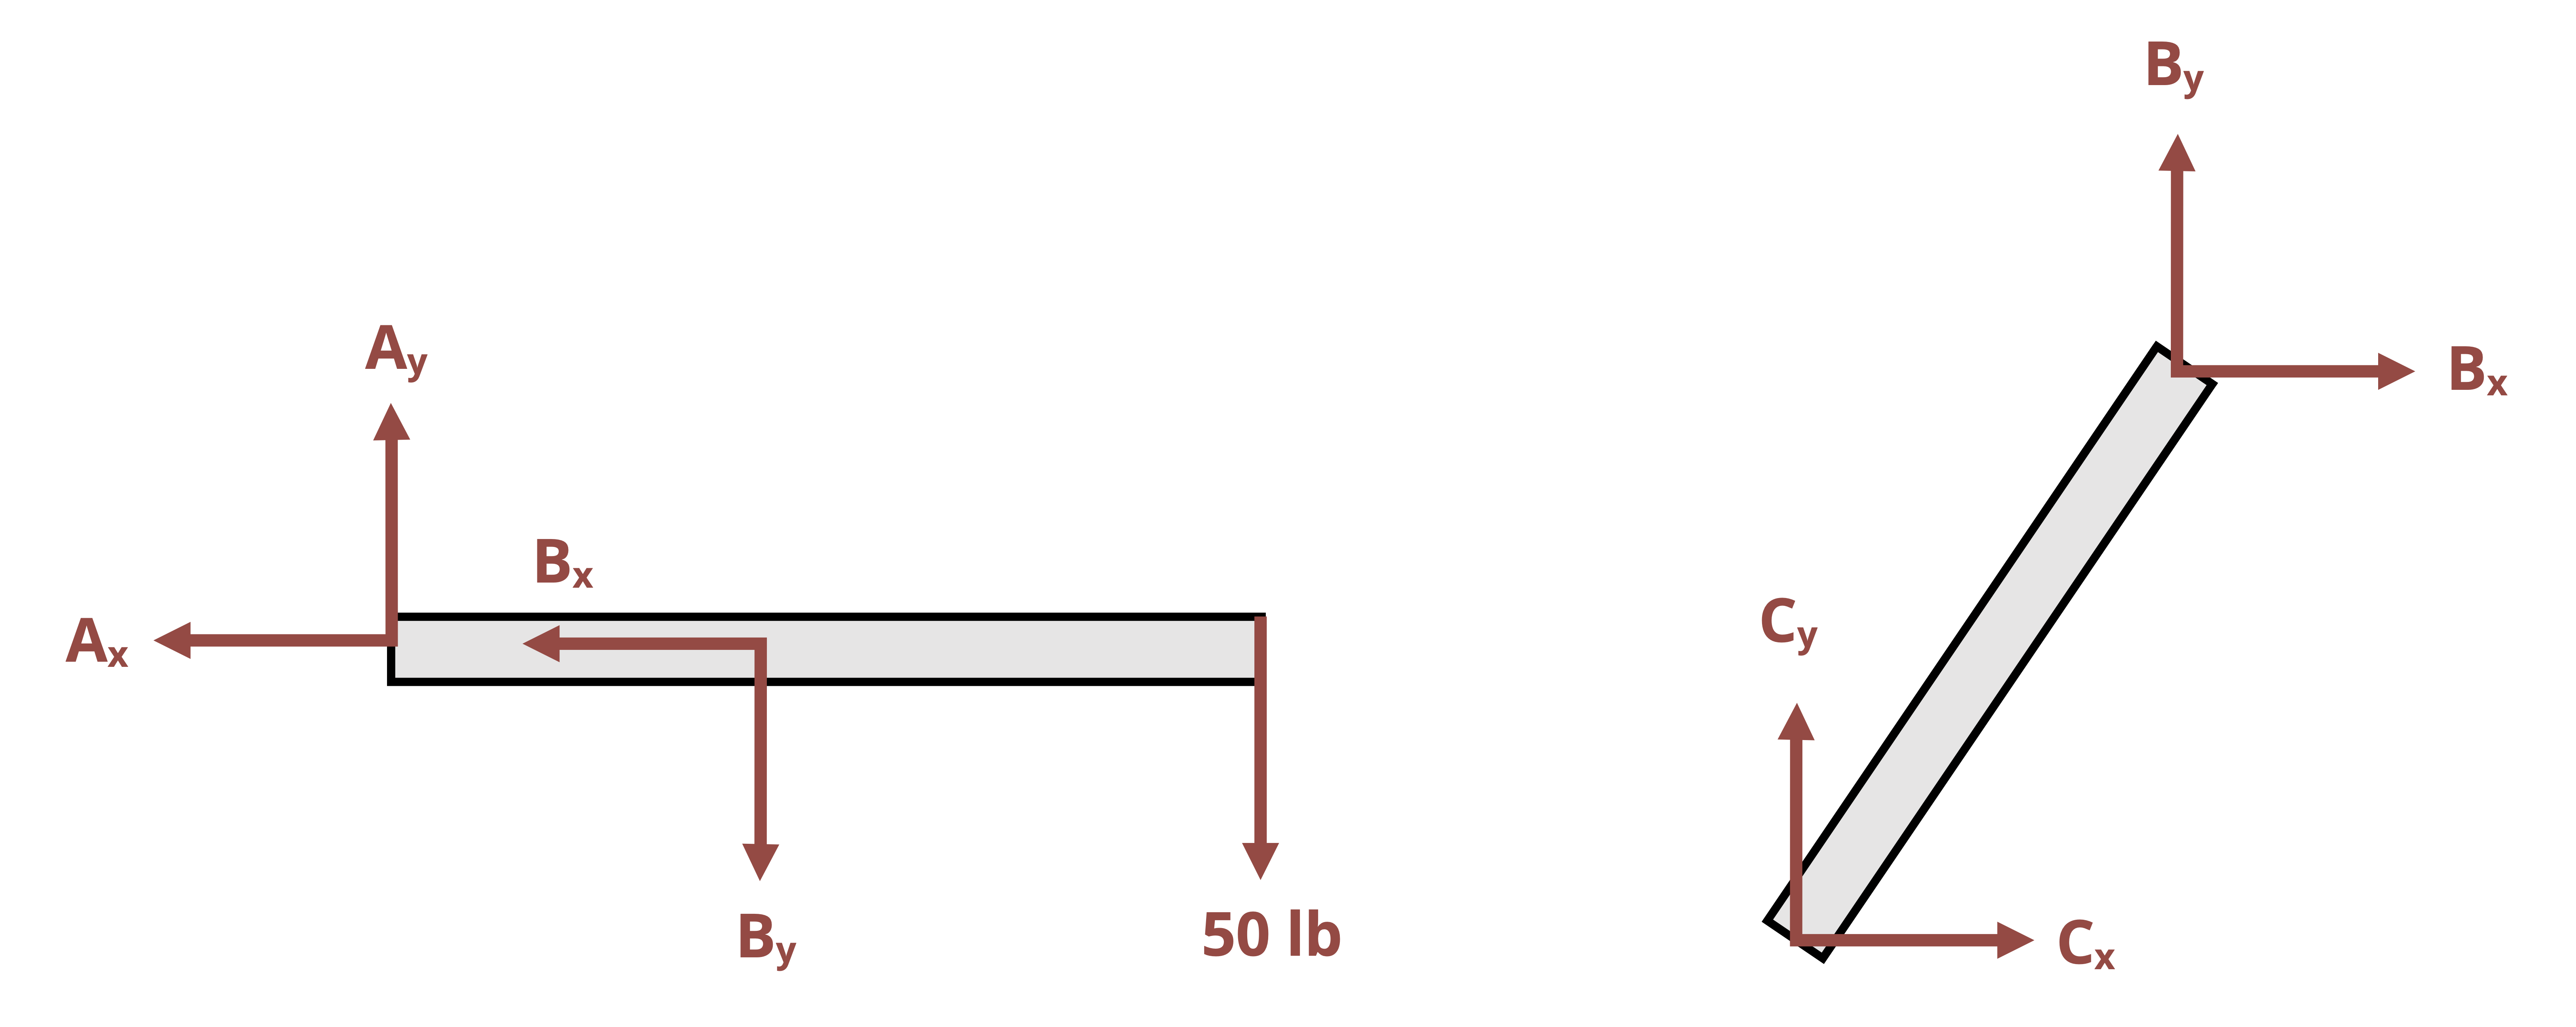
\includegraphics[width=5.86458in,height=\textheight]{images/CH1 PNGs/example 1.3 part 2.png}
\end{center}

There are now 6 unknowns and 6 equilibrium equations (3 equations per
body) available to use per bar, so the problem is technically solvable.
However, since BC is a two force member (there is a pin force at B and a
pin force at C but no other forces at any other point on the bar), it
can be taken as known that the reaction force at B follows a line of
action that goes through B and C. We can also conclude that the force in
pin C is equal to the force in pin B. The FBD of bar AB can be redrawn:

\begin{center}
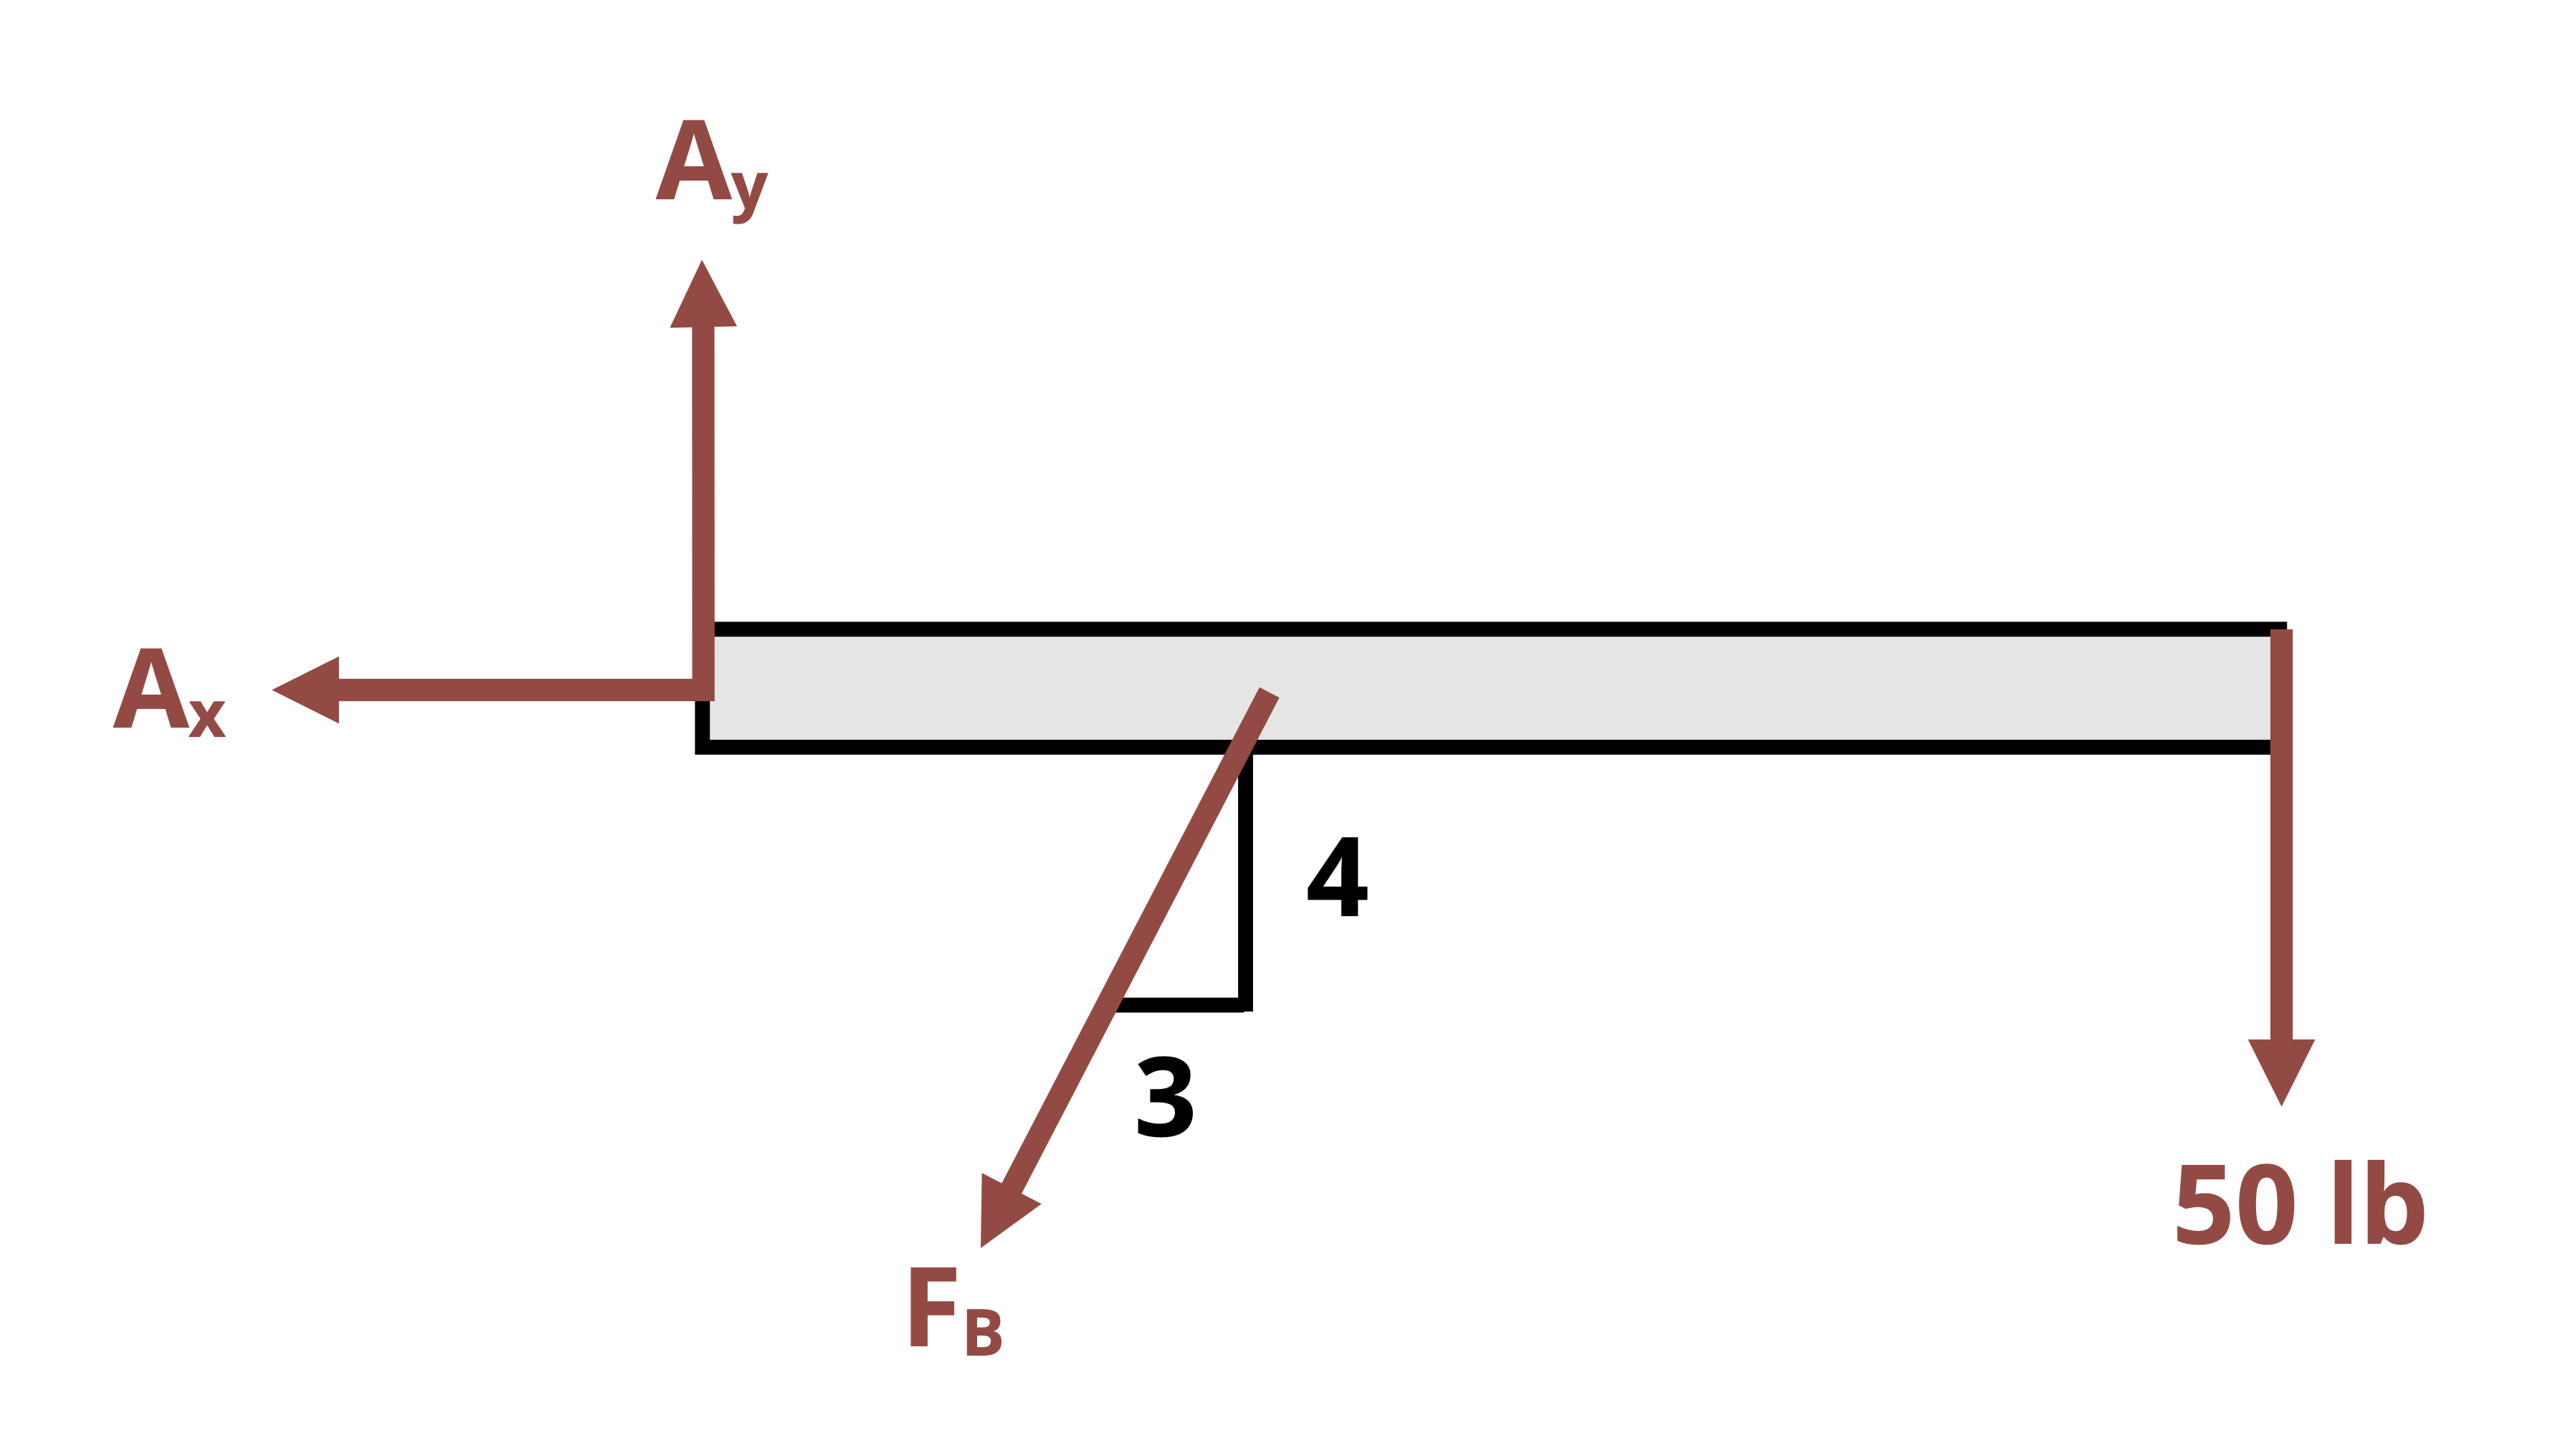
\includegraphics[width=3.1875in,height=\textheight]{images/CH1 PNGs/example 1.3 part 3.png}
\end{center}

With the components B\textsubscript{x} and B\textsubscript{y} replaced
with the resultant force F\textsubscript{B} with known direction, the
number of unknowns on bar AB is reduced to 3. These unknowns can be
solved for using the equilibrium equations:

\[
\begin{aligned}
\text{(1)} & \sum M_A=F_B\left(\frac{4}{5}\right) 3 f t-50 l b(7 f t)=0 \\
\text{(2)} & \sum F_x=-A_x+F_B\left(\frac{3}{5}\right)=0 \\
\text{(3)} & \sum F_y=A_y+F_B\left(\frac{4}{5}\right)-50 l b=0
\end{aligned}
\]

Solving the equations (1)-(3) yields F\textsubscript{B} = 145.8 lb,
A\textsubscript{x} = 87.5 lb, and A\textsubscript{y} = -66.7 lb.
Therefore, the pin force in pin B is 145.8 lb and the pin force in A is
\(\mathrm{A}=\sqrt{A_x^2+A_y^2}=110 \text{ lb}\). Since BC is a
two-force member, F\textsubscript{C} = F\textsubscript{B}.

\textbf{Answer: F\textsubscript{A} = 110 lb, F\textsubscript{B} =
F\textsubscript{C} = 146.8 lb}

\end{tcolorbox}

\subsection{Internal reactions in truss
structures}\label{internal-reactions-in-truss-structures}

Truss structures are made up of only two force members. The two main
methods of determining internal reactions in planar (2D) truss
structures are Method of Joints and Method of Sections. In using Method
of Joints, an FBD is drawn of the connecting pins (joints) within the
truss. Since all the members connected at any given pin will be
two-force members, the reactions can be drawn in known directions.
However, since the forces all pass through the same point on the body,
the moment equilibrium equation is not useful, so only the forces
equilibrium equations can be used for each joint. This means that only
two unknowns can be solved for at each joint. This method is most useful
when the forces of all the truss members are sought or if the only
forces sought are attached to a joint with only two members.

To use Method of Sections, a cut is made through the truss structure and
analysis is based on the FBD of the intact part of the structure that is
to the left of the cut or the intact part of the structure to the right
of the cut. The FBD of either given side will show the applied forces
and the reaction forces from the members that were cut through. These
reactions will be equal in magnitude but opposite in direction between
the two sides of the cut. The side to examine is usually based on which
one will not require having to find external reactions (if there is a
free end to the truss) and/or which one is least complicated to deal
with in terms of geometry or applied loads. All three equilibrium
equations can generally be effectively applied with Method of Sections,
so three unknowns can be solved for with any given cut.

Example 1.4 demonstrates the use of both Method of Joints and Method of
Sections to solve for forces in truss members.

\begin{tcolorbox}[enhanced jigsaw, colback=white, colframe=quarto-callout-note-color-frame, leftrule=.75mm, opacitybacktitle=0.6, colbacktitle=quarto-callout-note-color!10!white, arc=.35mm, bottomrule=.15mm, breakable, title={Example 1.4}, left=2mm, titlerule=0mm, toptitle=1mm, toprule=.15mm, opacityback=0, rightrule=.15mm, coltitle=black, bottomtitle=1mm]

Determine the forces in members ED and EF. Let P\textsubscript{1} = 8 kN
and P\textsubscript{2} = 12 kN.

\begin{center}
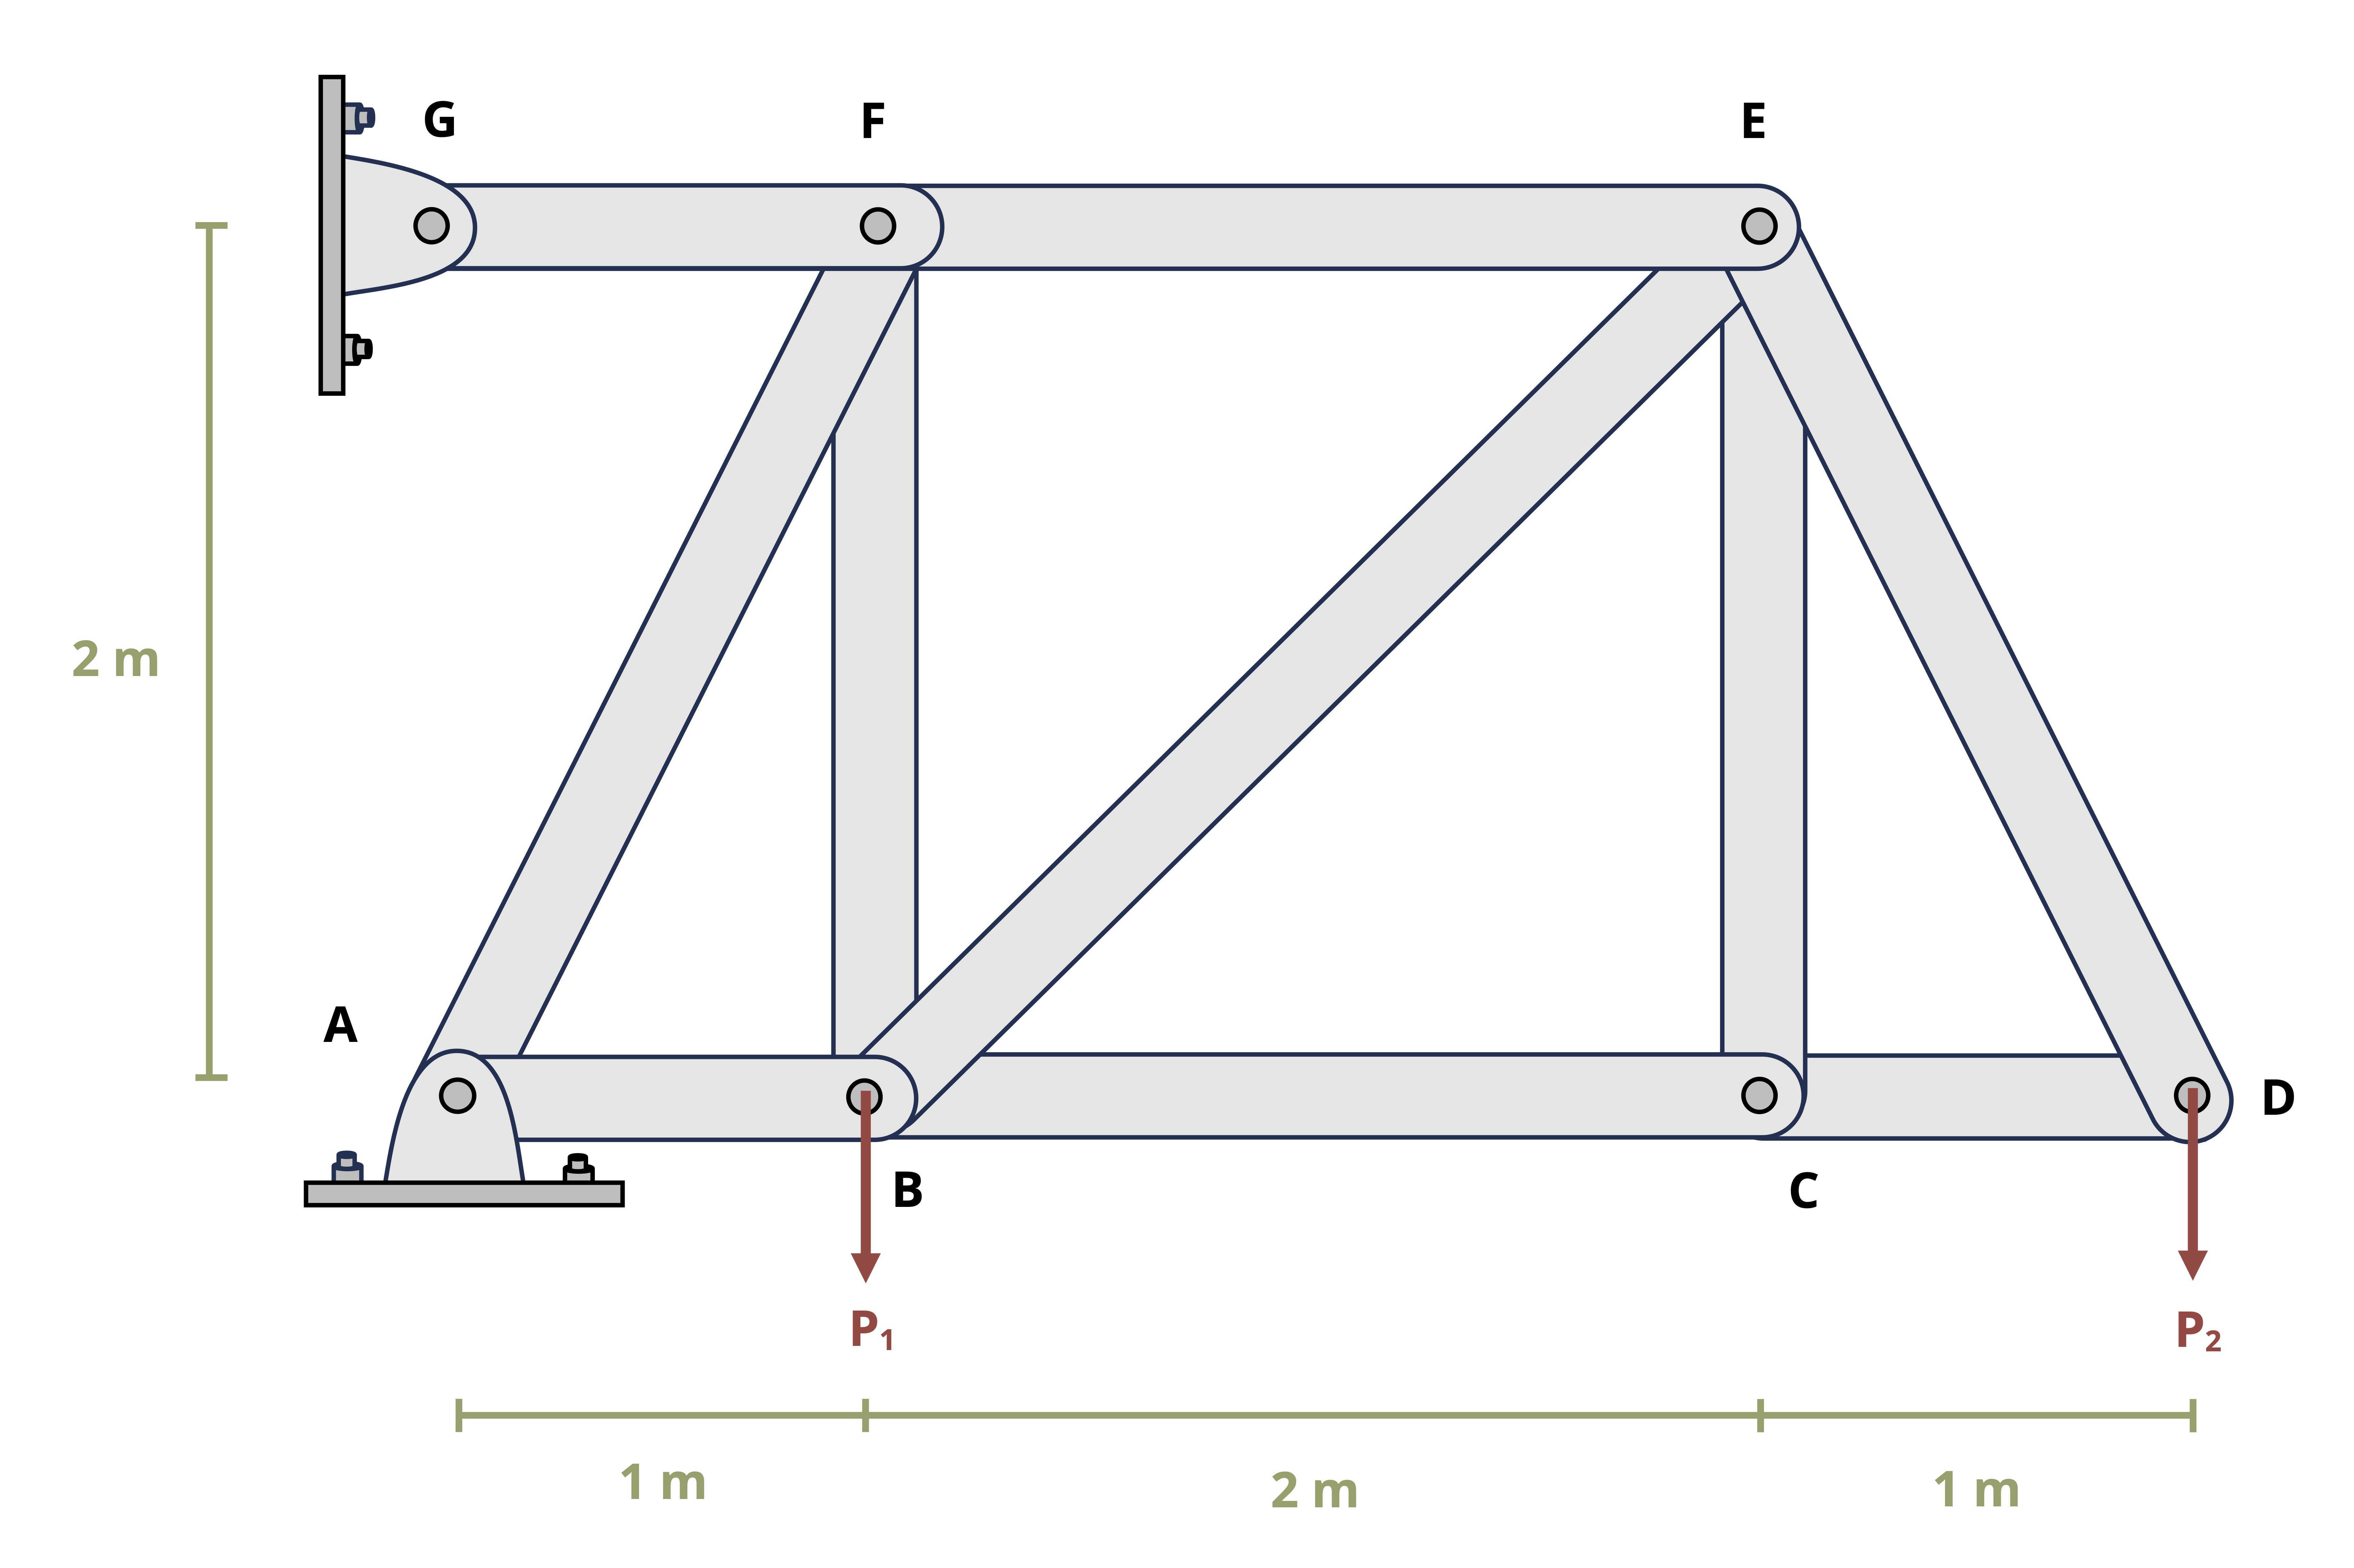
\includegraphics{images/CH1 PNGs/example 1.4 part 1.png}
\end{center}

Considering Joint E, it can be seen that since there are 4 members
attached to the joint, there would be 4 unknown forces to account for.
Therefore, starting with Method of Joints at E would not work. However,
looking at joint D, there are only two unknowns, with one of them being
member ED, so that would be a useful place to start.

\textbf{FBD Joint D}

Note: The triangle ECD is a right triangle, so the sin and cos of the
angle at corner D can be expressed in terms of the ratios of the sides.
If the angle at D is θ, then cos(θ)= \(\frac{1}{\sqrt{5}}\) and sin(θ)=
\(\frac{2}{\sqrt{5}}\) where \(\sqrt{5}\) is the hypotenuse of the
triangle.

\[
\begin{aligned}
\text{(1)} & \sum F_x=-F_{C D}-F_{D E}\left(\frac{1}{\sqrt{5}}\right)=0 \\
\text{(2)} & \sum F_y=F_{D E}\left(\frac{2}{\sqrt{5}}\right)-12 k N=0
\end{aligned}
\]

\begin{center}
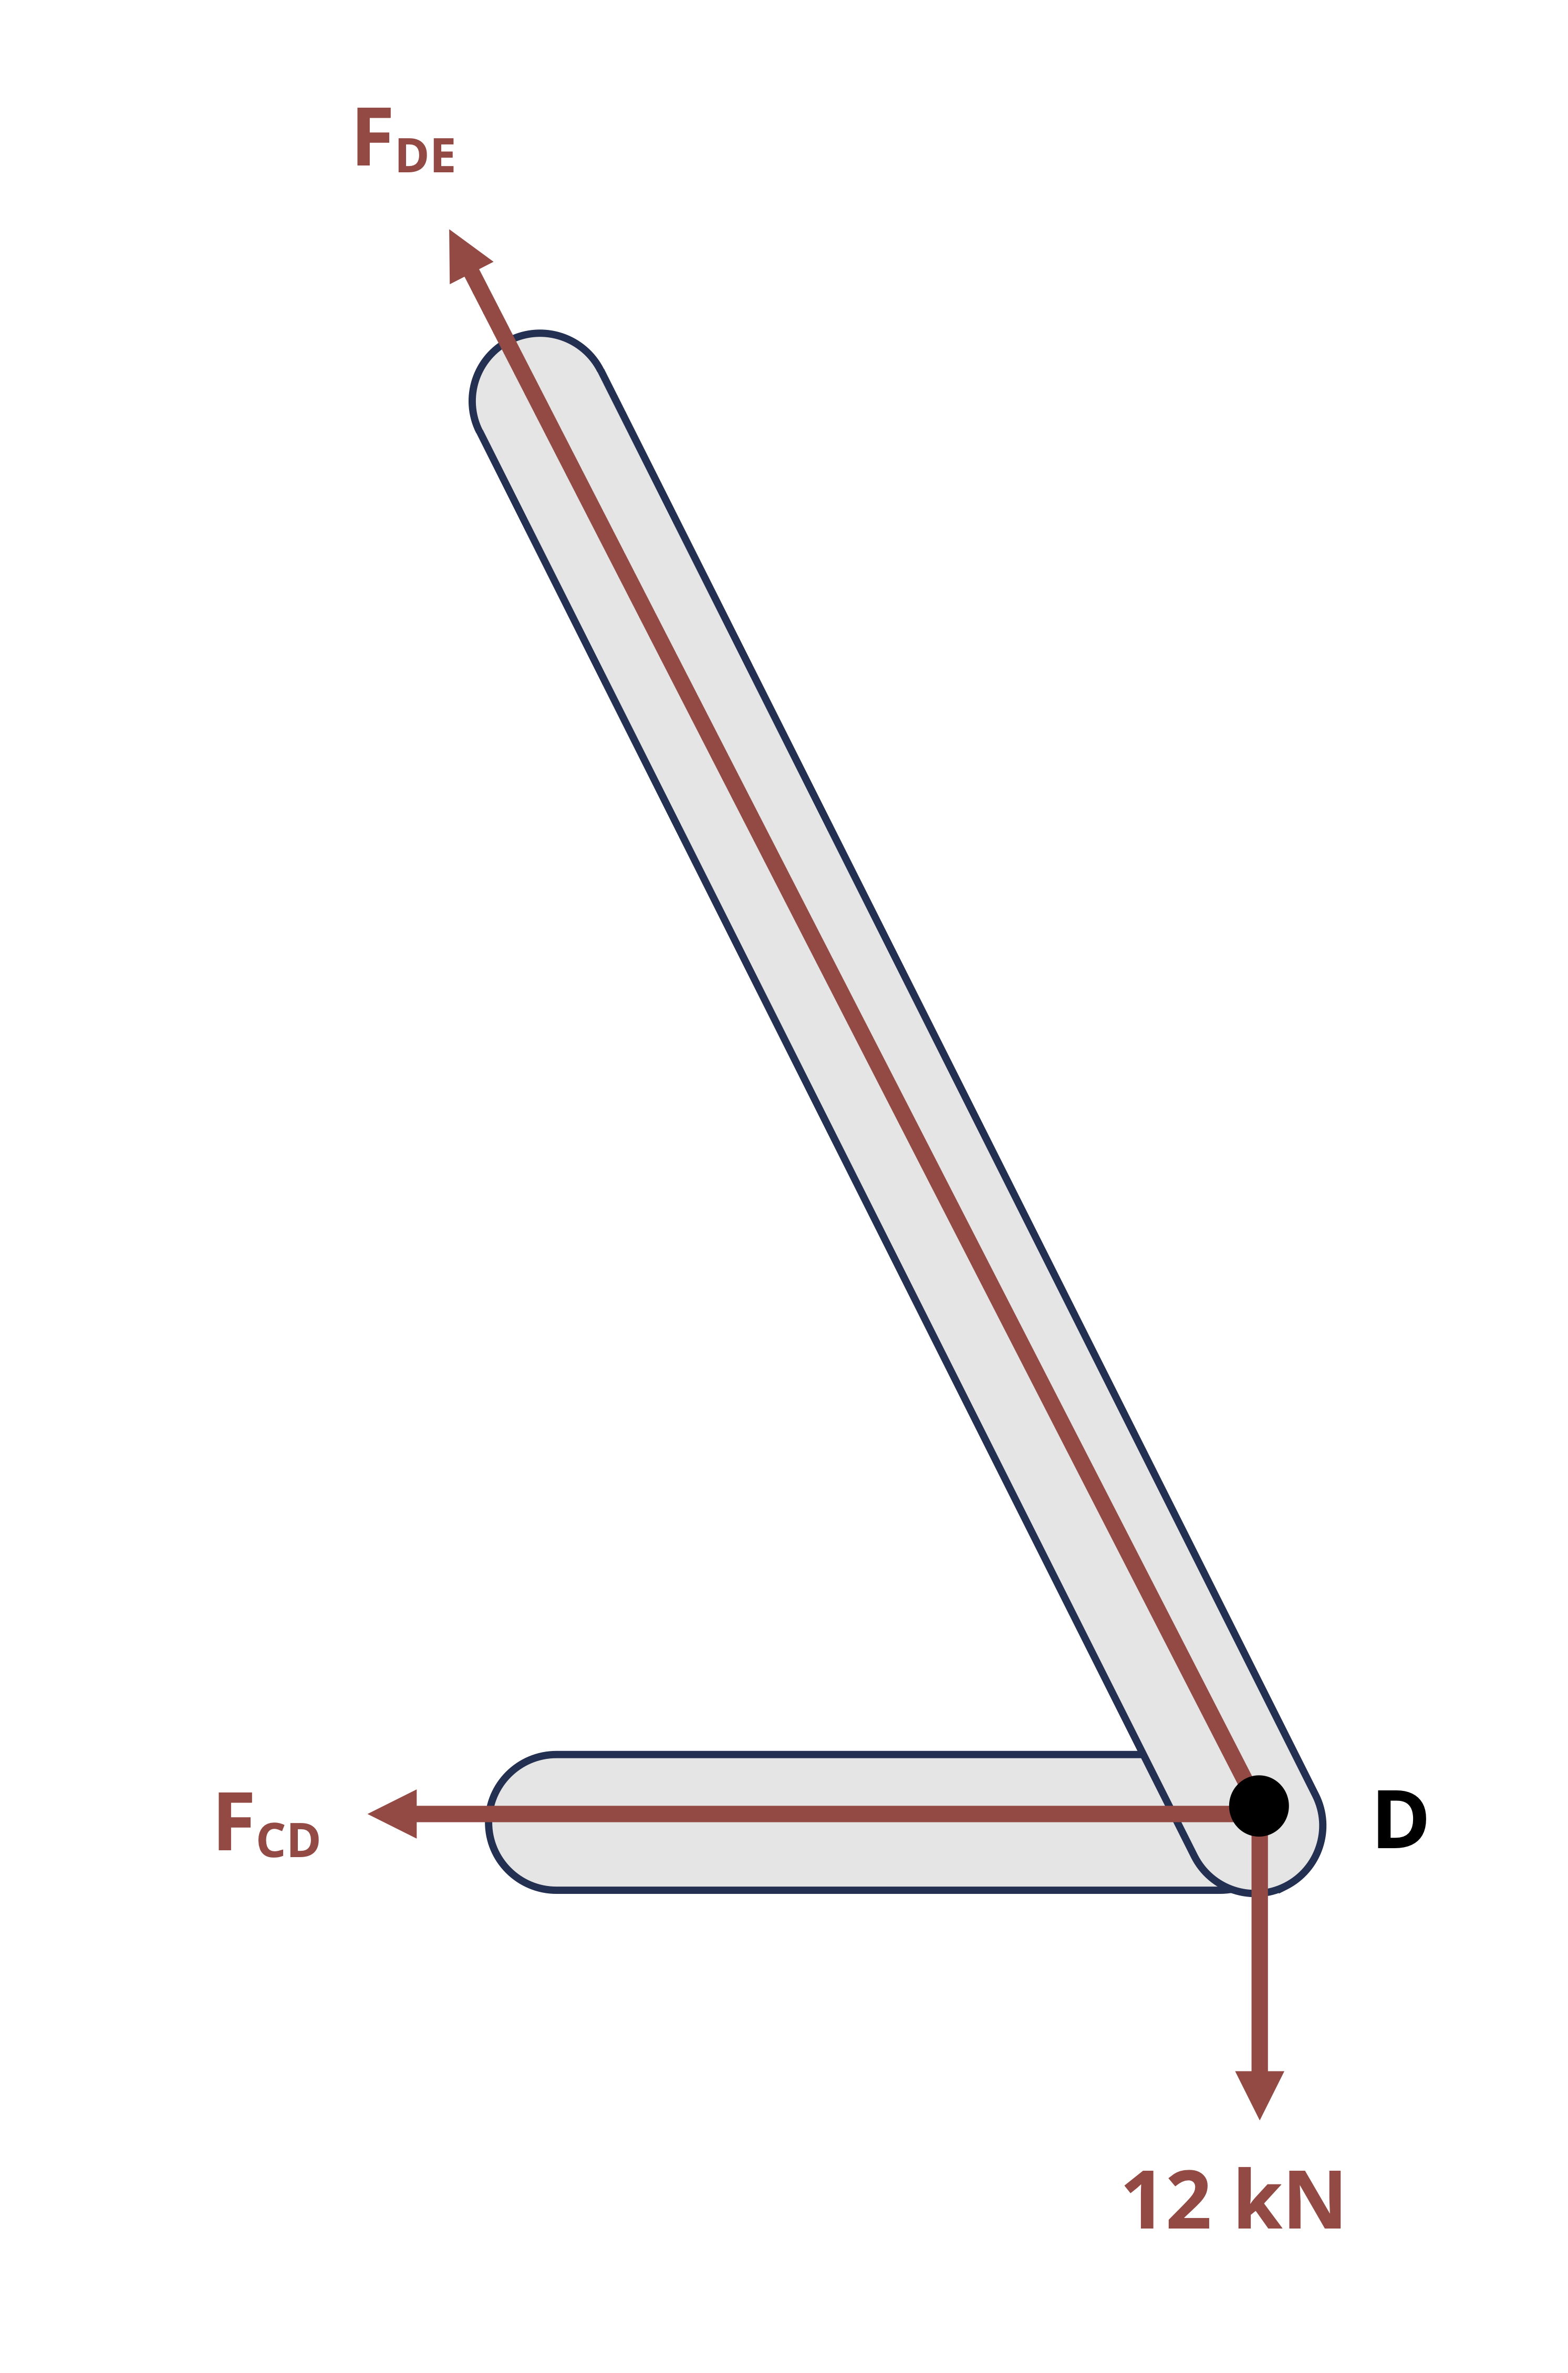
\includegraphics[width=2.3125in,height=\textheight]{images/CH1 PNGs/example 1.4 part 2.png}
\end{center}

Solving (1) and (2) gives F\textsubscript{DE} = 13.42 kN (tensile) and
F\textsubscript{DC} = -6 kN.

Since the force is shown to be tensile in the FBD (the force is pointed
away from the joint), the negative answer indicates the force is
actually compressive.

Even with knowing F\textsubscript{DE}, joint E would have three unknown
forces. Joint C only has two unknown forces, so we can draw that joint
next. Note that we previously determined F\textsubscript{CD} = 6 kN in
compression, so we will draw that force in compression at joint C.
Forces F\textsubscript{BC} and F\textsubscript{CE} are unknown and may
be drawn in either direction. For this example they've been drawn in
tension.

\begin{center}
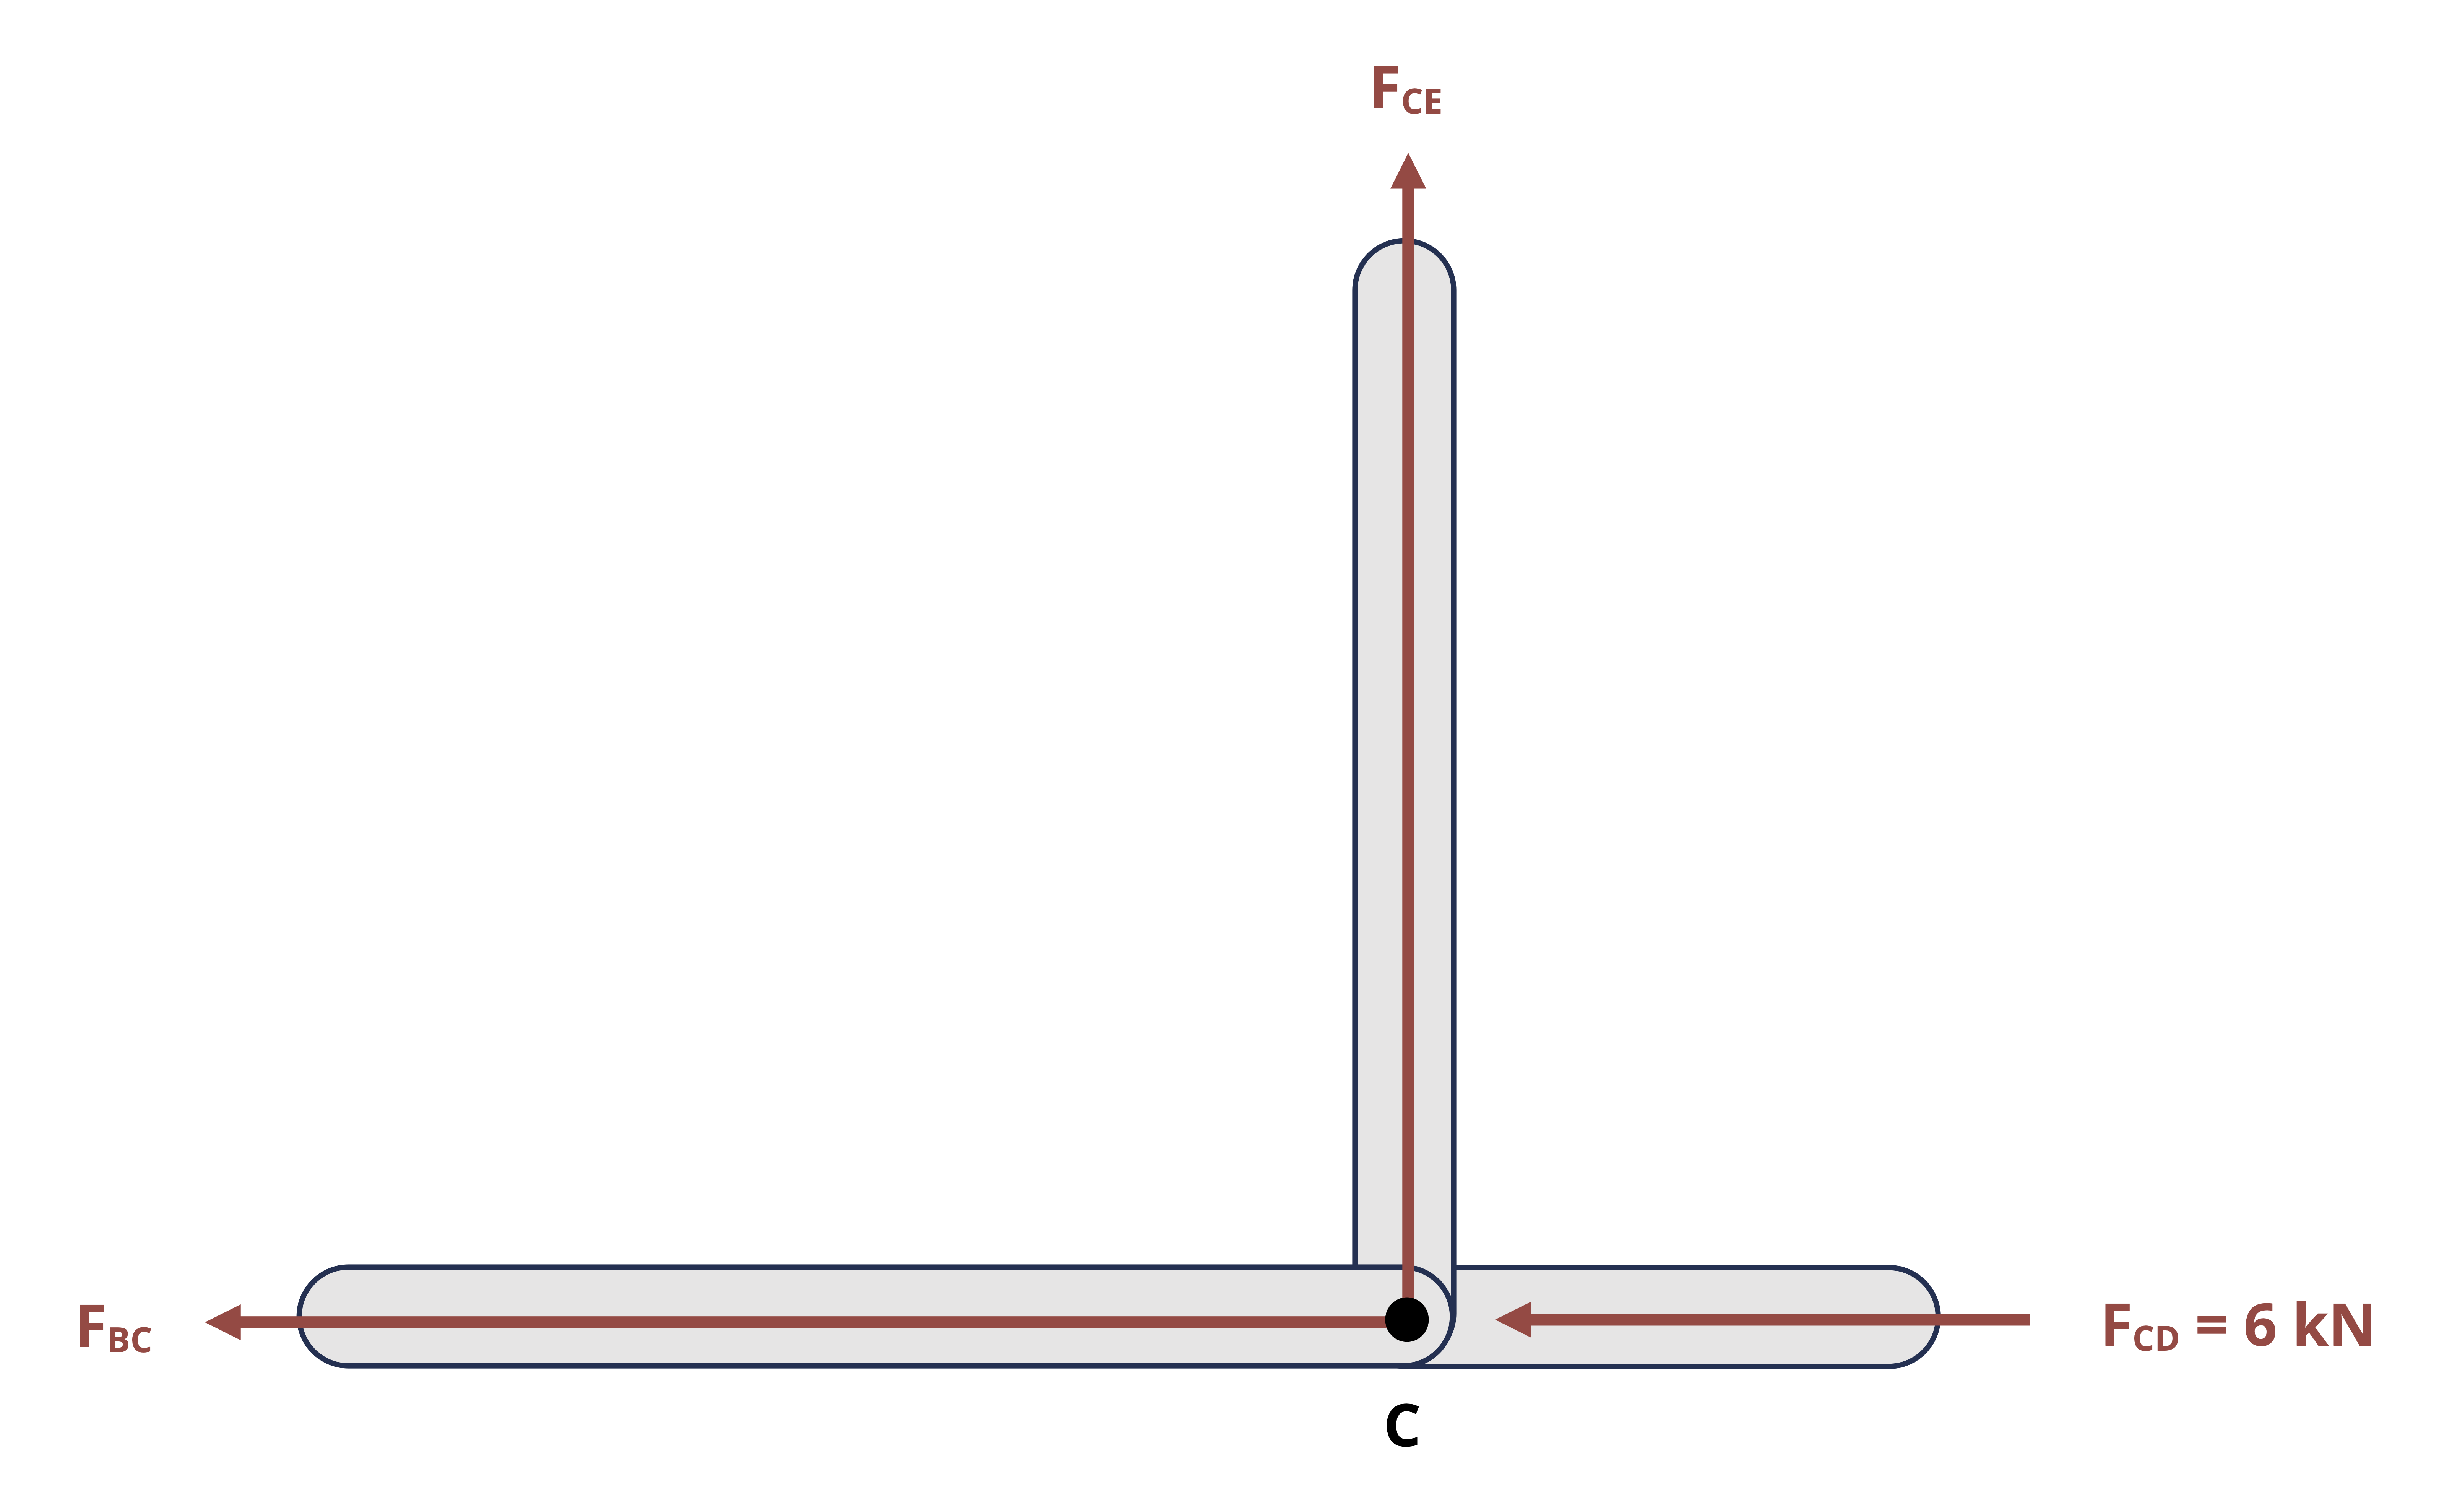
\includegraphics[width=5.34375in,height=\textheight]{images/CH1 PNGs/example 1.4 part 3.png}
\end{center}

\[
\begin{aligned}
&\sum F_x=-F_{B C}-6=0 \rightarrow F_{B C}=-6 k N\\
&\sum F_y=F_{C E}=0
\end{aligned}
\]

Then at joint E:

\begin{center}
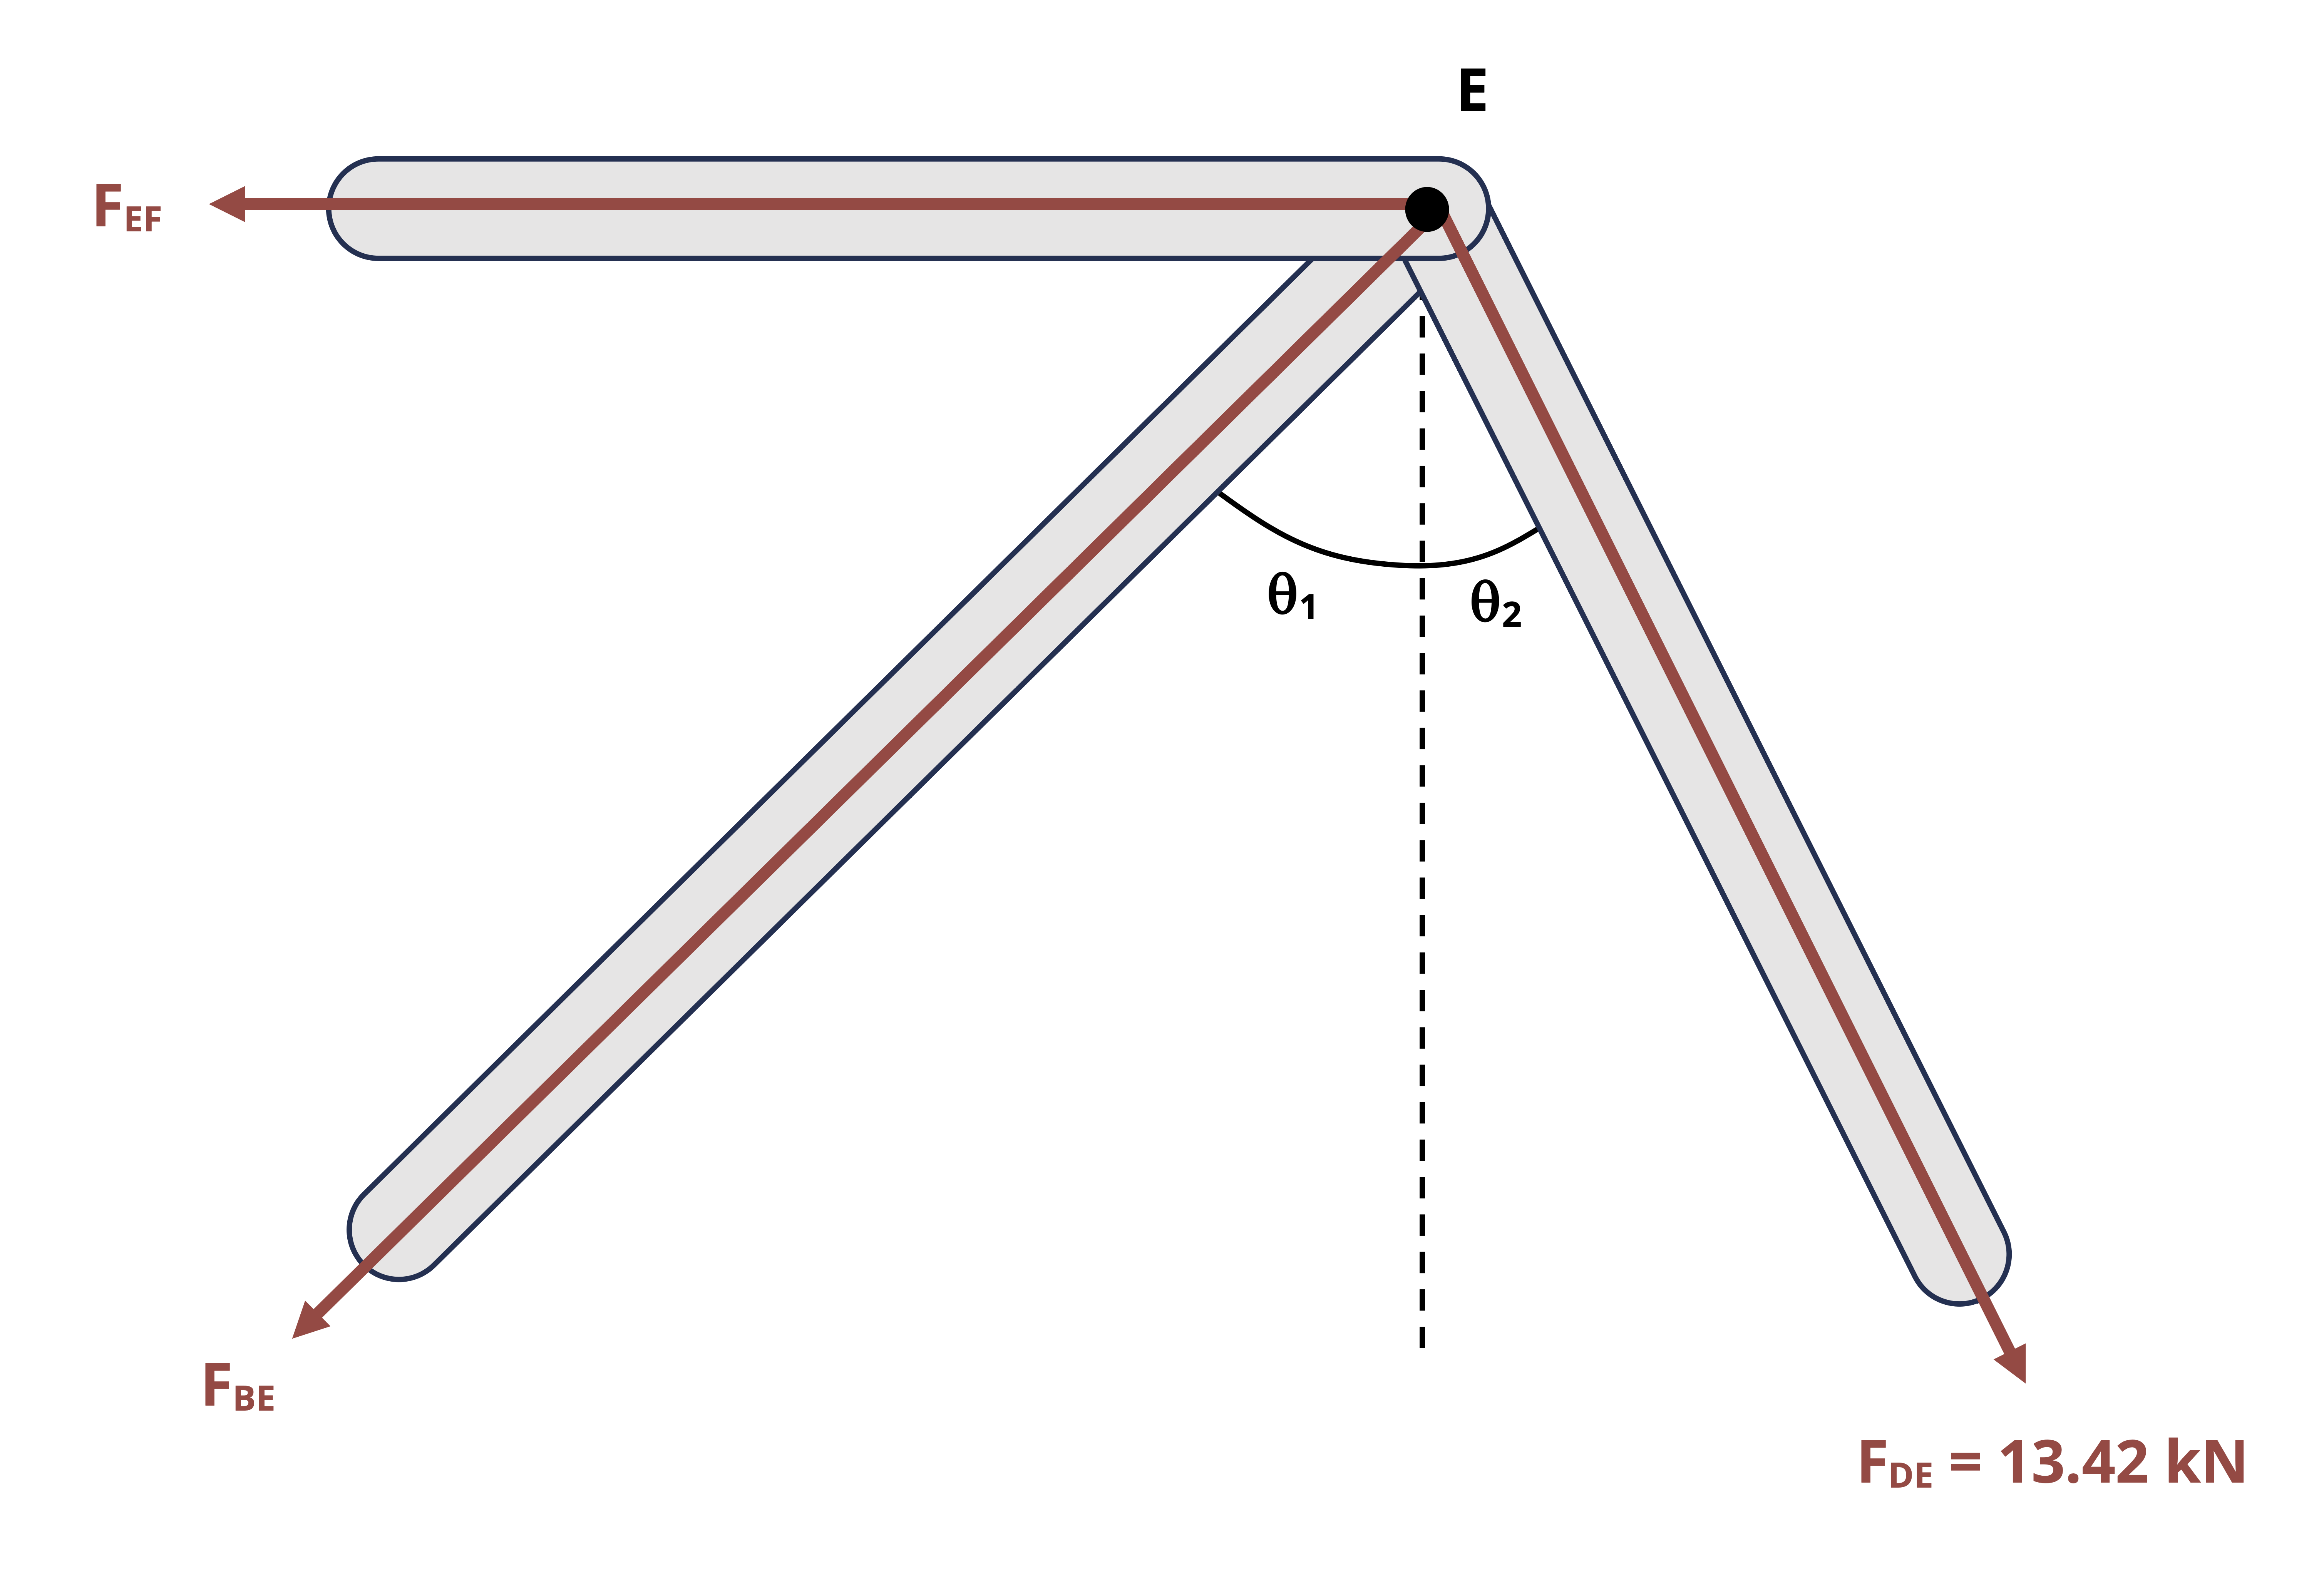
\includegraphics[width=4.84375in,height=\textheight]{images/CH1 PNGs/example 1.4 part 4.png}
\end{center}

\[
\begin{aligned}
&\sum F_y=-13.42\left(\frac{2}{\sqrt{5}}\right)-F_{B E}\left(\frac{2}{\sqrt{8}}\right)=0 \rightarrow F_{B C}=-16.98 k N\\
&\sum F_x=13.42\left(\frac{1}{\sqrt{5}}\right)--16.98\left(\frac{2}{\sqrt{8}}\right)-F_{E F}=0 \rightarrow F_{E F}=18 \mathrm{kN}
\end{aligned}
\]

\textbf{Answer: FDC = 6 kN (Compressive), FEF = 18 kN (Tensile)}

While Method of Joints can be used here, it is inefficient. We needed to
draw and analyze free body diagrams of joints D, C, and E and keep track
of the forces at these joints as well as whether each force was in
tension or compression.

Method of Sections may be used as an alternative to find force FEF. To
apply Method of Sections for this problem, a cut will be made through
the truss that passes vertically through members EF, BE, and BC. Once
that cut is made, a choice needs to be made to draw an FBD for the
intact part of the truss to the left of the cut (everything to the left
of BF in this case) or the intact part of the truss to the right of the
cut (everything to the right of EC in this case). Either way, the
external forces on the side would need to be shown on the FBD as well as
the force of each member that was cut through. This is illustrated
below. Notice that the forces are drawn in opposite directions on the
different sides of the cut.

\begin{center}
\includegraphics{images/CH1 PNGs/example 1.4 part 5.png}
\end{center}

Looking at the FBD of the two cut sections, the right side section would
be easiest to work with since there are no external reactions on that
side. If the left side section were picked, the reactions at A and G
would first need to be determined (note that FGF = Gx). All three
equilibrium equations can be used with the Method of Sections. In this
particular case in which only EEF is left to solve for, only the moment
about B is needed to solve since the other two unknown forces both pass
through B.

\[
\sum M_B=-P_2(3 m)+F_{E F}(2 m)=0 \rightarrow F_{E F}=18 \text{ kN}
\]

Once again, the forces are drawn on the FBD in the tensile direction, so
the negative answer indicates a compressive force.

\textbf{Answer: FDC = 6 kN (Compressive), FEF = 18 kN (Tensile)}

\end{tcolorbox}

\subsection{Internal reactions in continuous
bodies}\label{internal-reactions-in-continuous-bodies}

Internal reactions also exist within a body or structure. These
reactions are necessary to hold the body together and will vary from
point to point in a body depending on the distribution of external
loading. As shown in Figure 1.2, the reactions at any given point can be
examined by making a cut at the point of interest in the body. One can
think of any point within a body as acting as a fixed support for the
rest of the body. That is, every point must potentially exert a force
parallel to the cross section where the cut is made which is the shear
force V, a force perpendicular to the cross section where the cut is
made which is the normal force N, and a reaction moment where the cut is
made which is the bending moment M. Moreover, as was discussed for
internal pin reactions and the cut made for Method of Sections for
trusses, the reactions at a cut will be equal and opposite on the two
sides of the cut.

\begin{center}
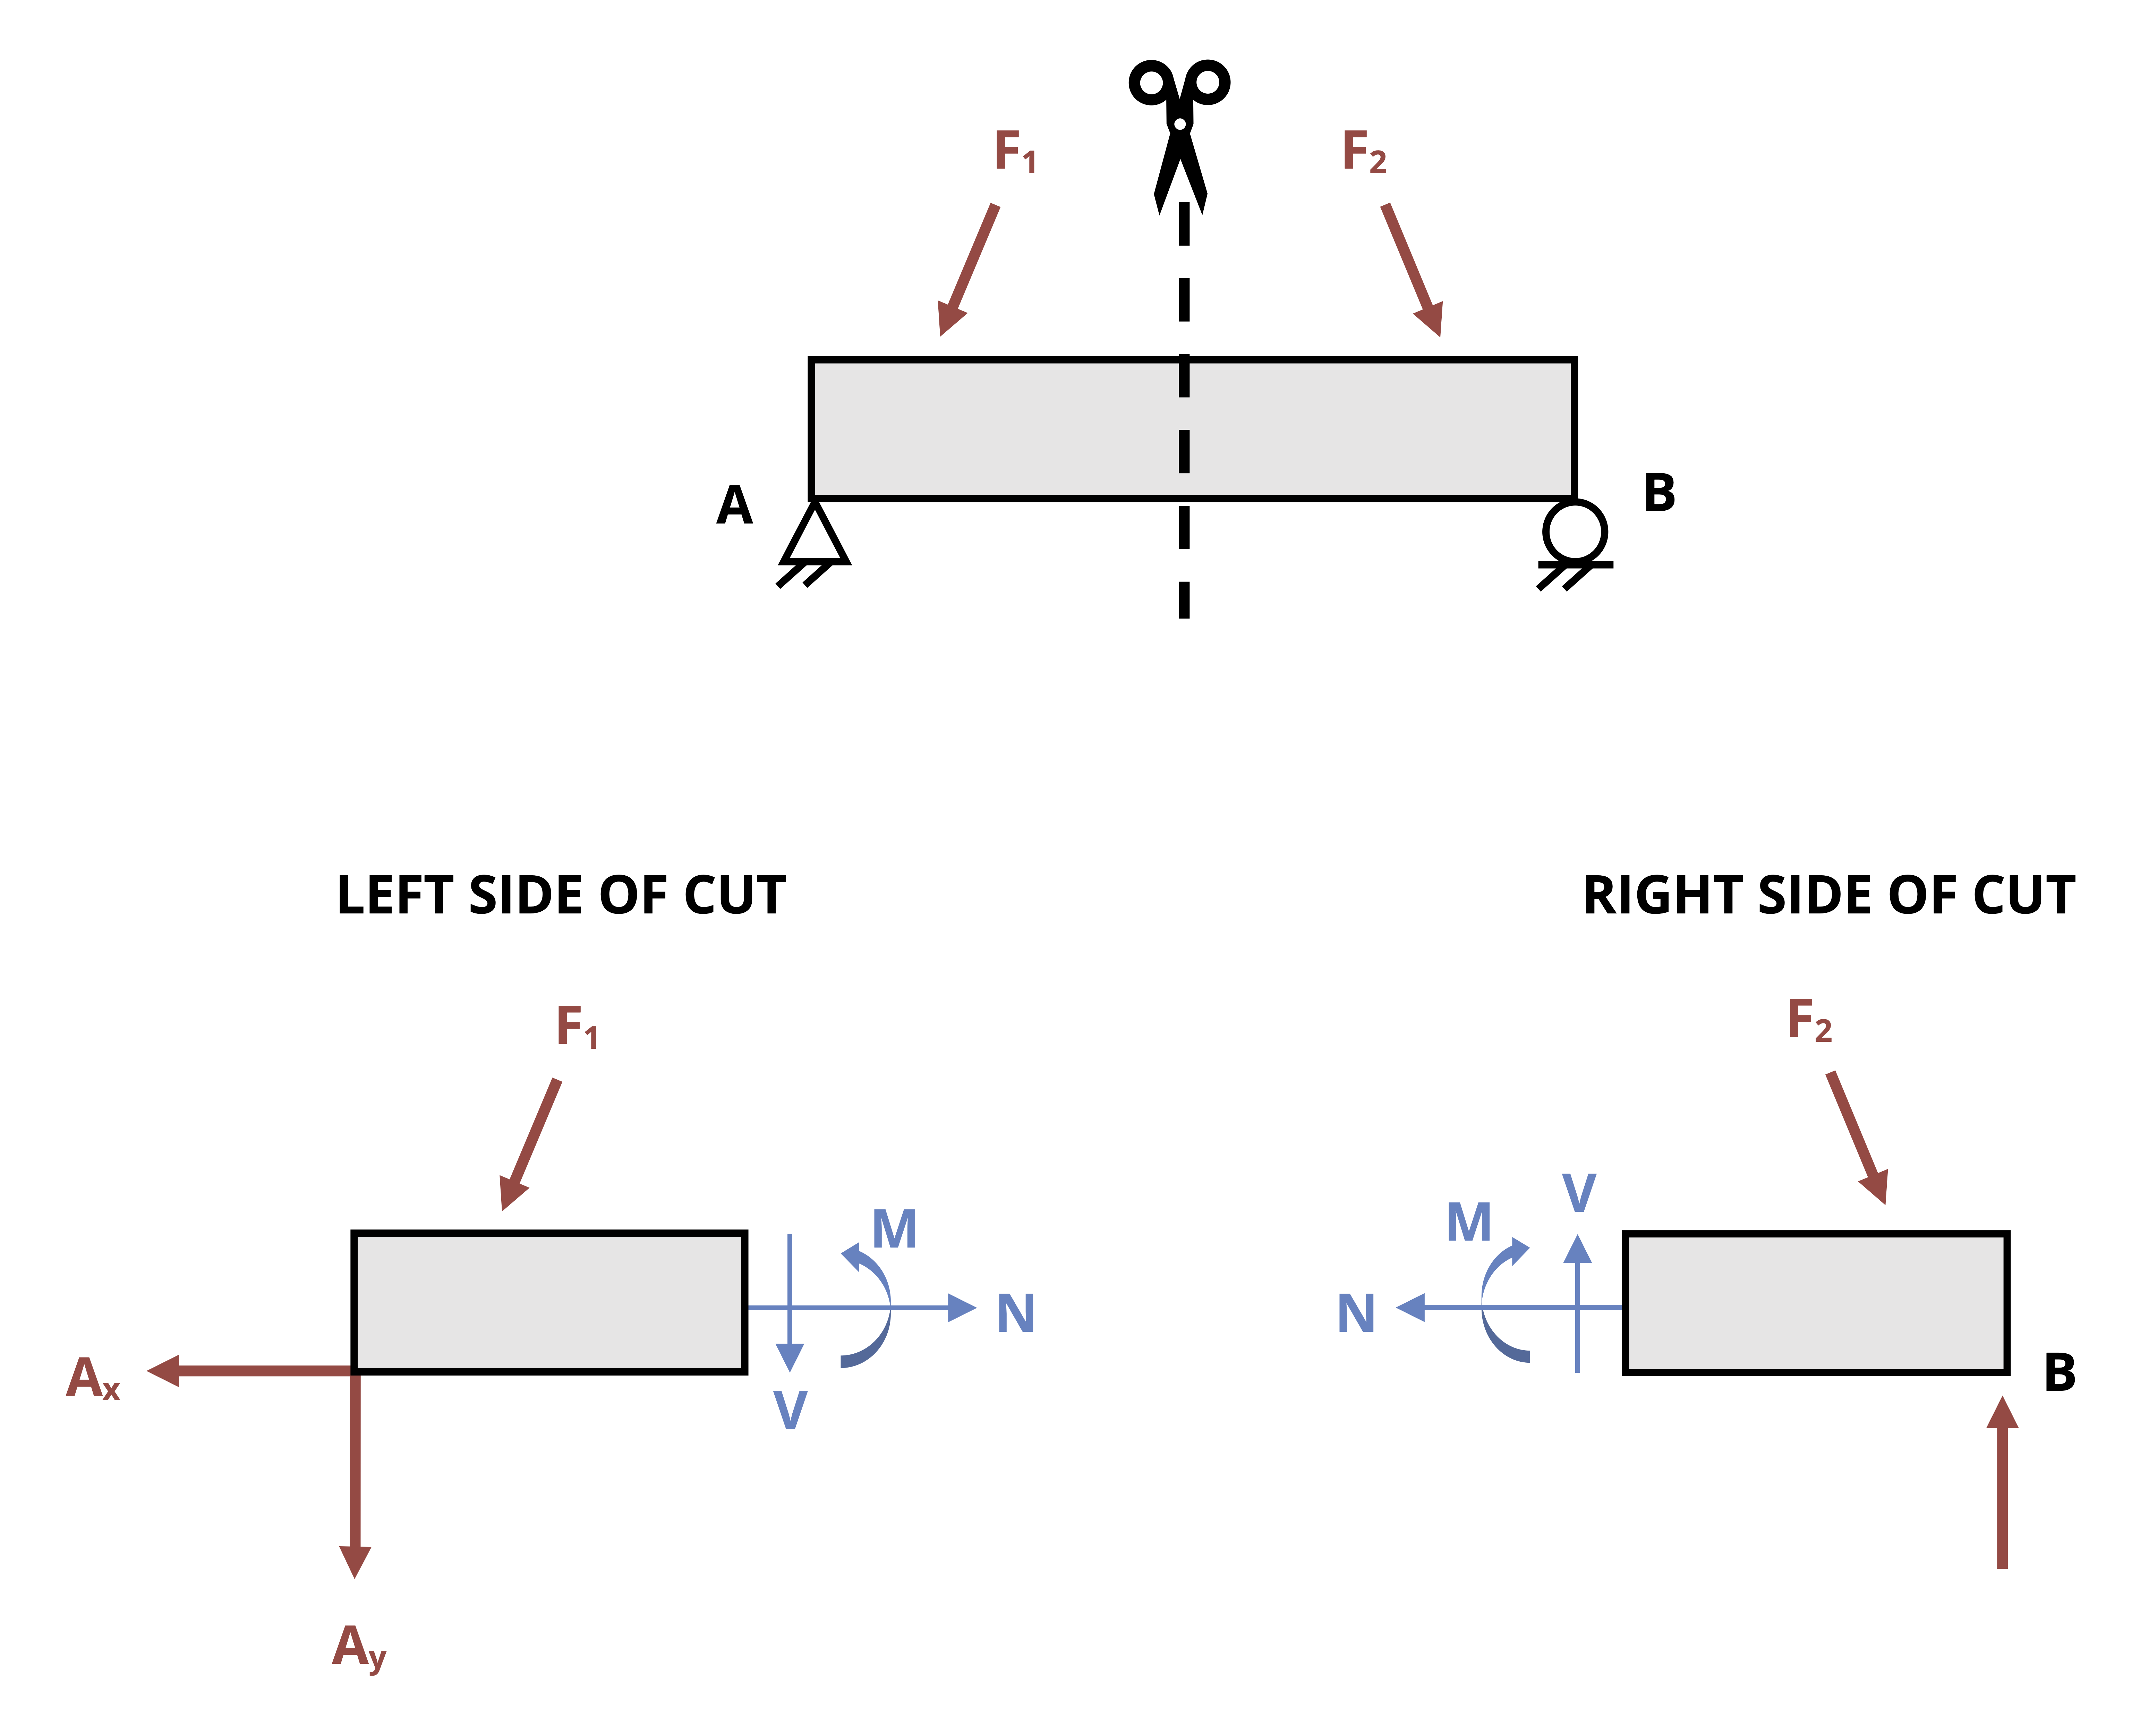
\includegraphics[width=5.03125in,height=\textheight]{images/CH1 PNGs/figure 1.2.png}
\end{center}

To determine the reactions, the FBD of the part of the beam to the left
of the cut can be drawn and used, or the part of the beam to the right
of the cut can be drawn and used. As was discussed with Method of
Sections for trusses, the choice of which side of the cut to examine is
based primarily on which side appears easiest and most efficient to
analyze. Once the FBD of the cut section is drawn, the three equilibrium
equations can be applied to determine the internal reactions. The
determination of shear and bending moments in beams will be reviewed in
more detail in Chapter 8. The focus of Example 1.5 is on the
determination of the normal force, as this will be important in Chapters
2 and 3.

\begin{tcolorbox}[enhanced jigsaw, colback=white, colframe=quarto-callout-note-color-frame, leftrule=.75mm, opacitybacktitle=0.6, colbacktitle=quarto-callout-note-color!10!white, arc=.35mm, bottomrule=.15mm, breakable, title={Example 1.5}, left=2mm, titlerule=0mm, toptitle=1mm, toprule=.15mm, opacityback=0, rightrule=.15mm, coltitle=black, bottomtitle=1mm]

Two solid bars make up the axial assembly loaded as shown. Determine the
normal force in each bar. State whether the force is tensile or
compressive.

\begin{center}
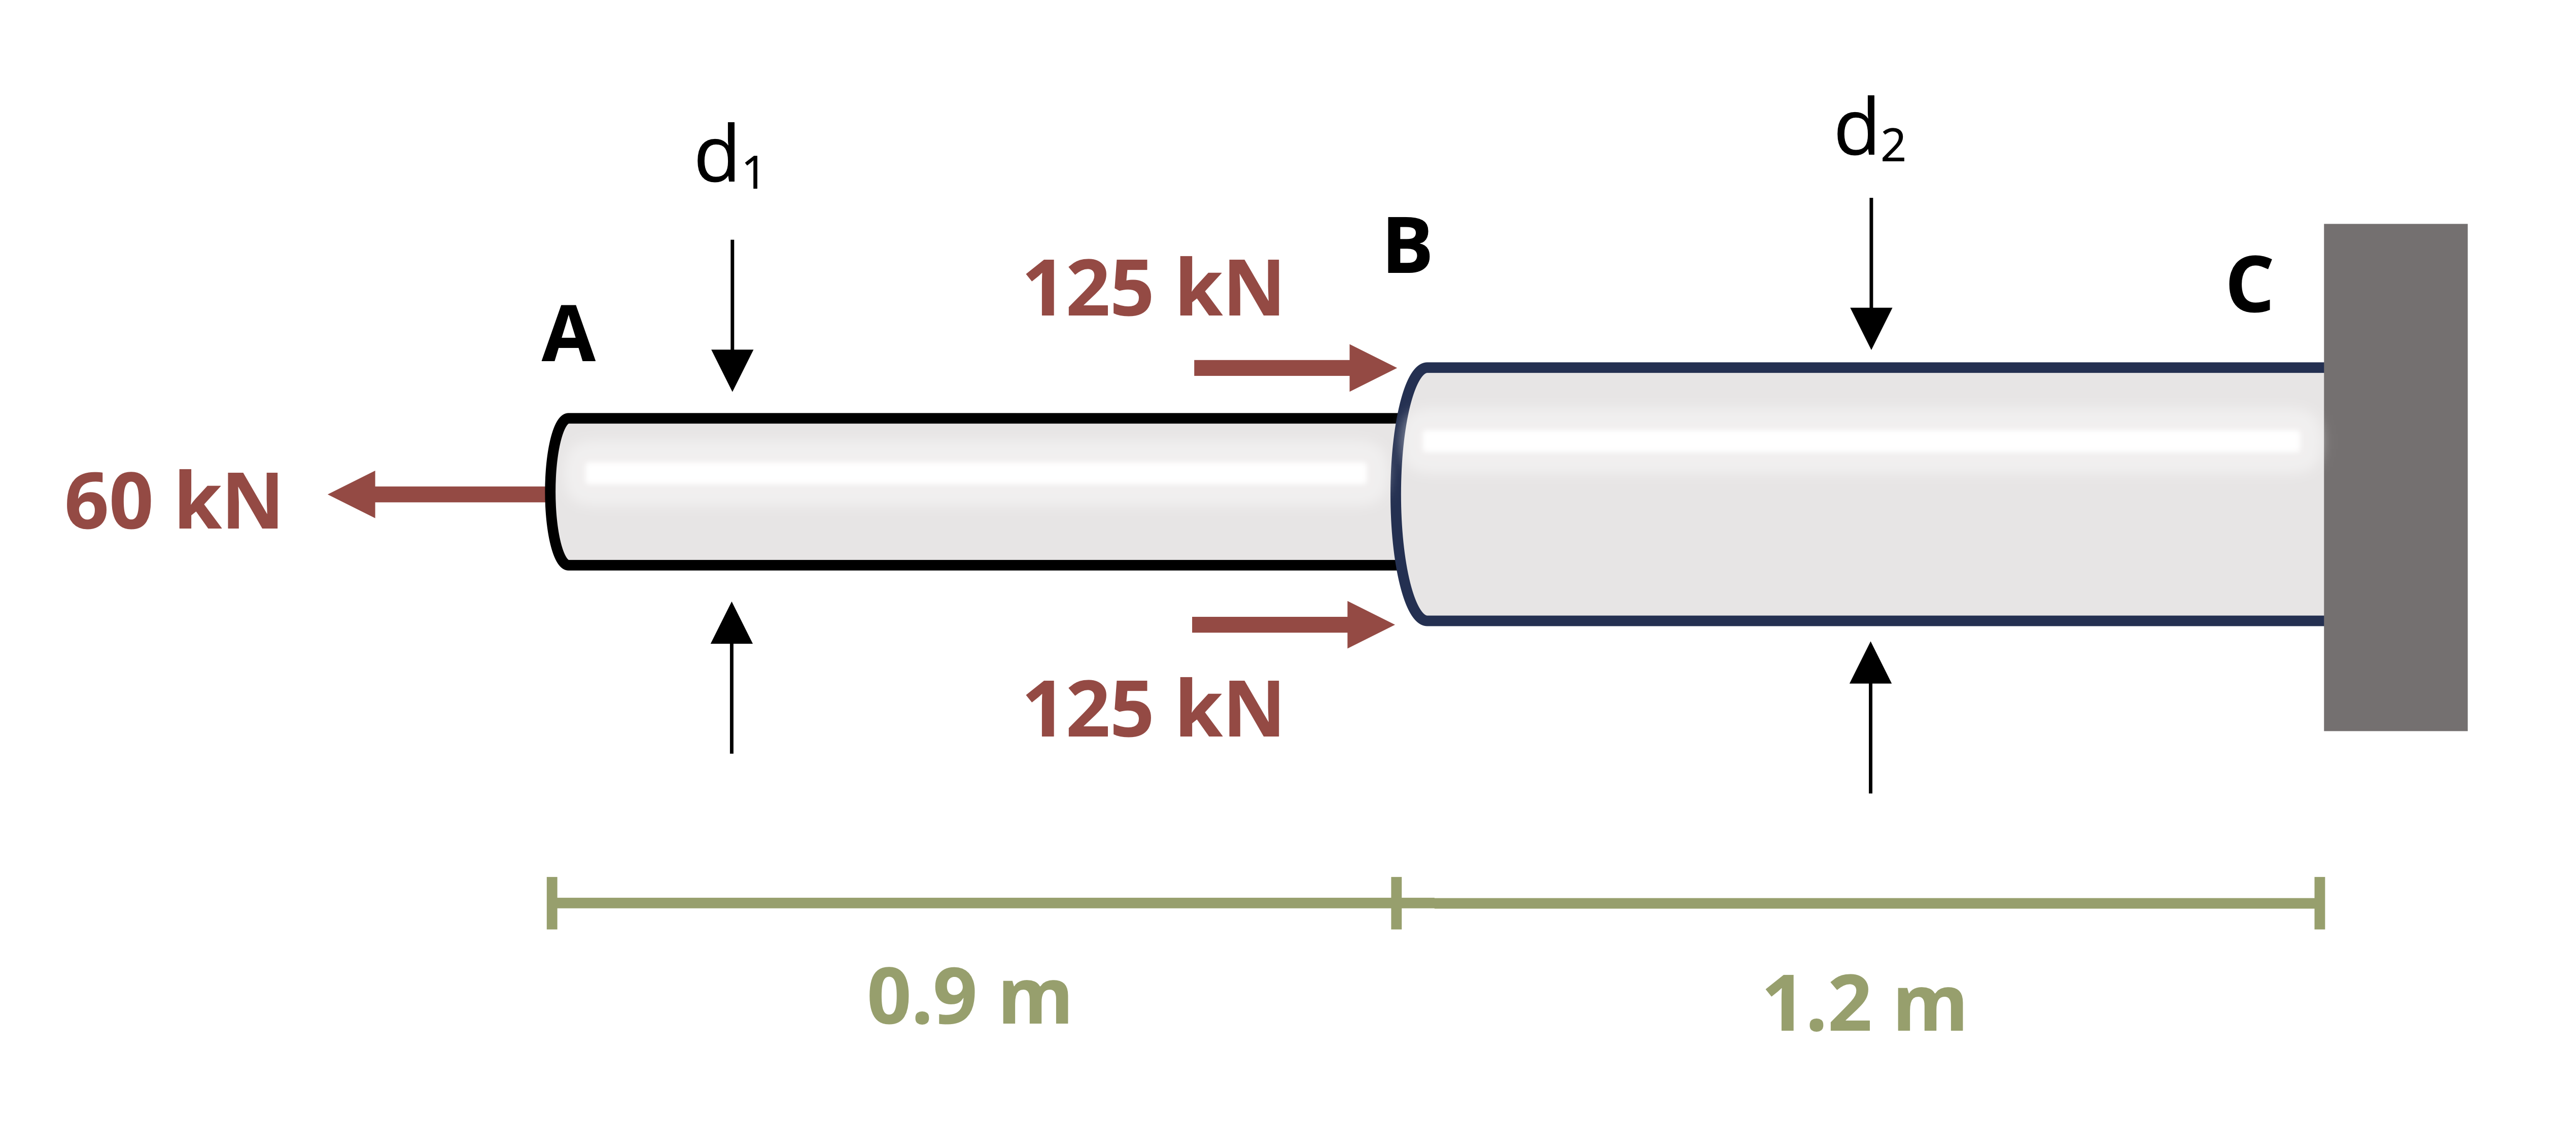
\includegraphics[width=4.16667in,height=\textheight]{images/CH1 PNGs/example 1.5 part 1.png}
\end{center}

Though the assembly is not a beam, determining the internal reactions
will work in the same way. In this particular case, all the forces are
in the normal direction (no shear force) and due to the central
placement of the 60 kN force and the symmetry of the 125 kN forces,
there will be also be no bending moment. Consequently, only the normal
reaction force will be drawn on the FBDs.

You may recall from shear and moment analysis of beams, a cut is made
whenever there is a loading change. In this example, there is a loading
change at B, so there will be two sections of the assembly with distinct
normal reactions.

Making the cut in section AB and drawing the FBD allows us to determine
the normal force in section AB. Note that drawing the left section of
the cut for the FBD results in avoiding needing to know the external
reactions at wall C.

\begin{center}
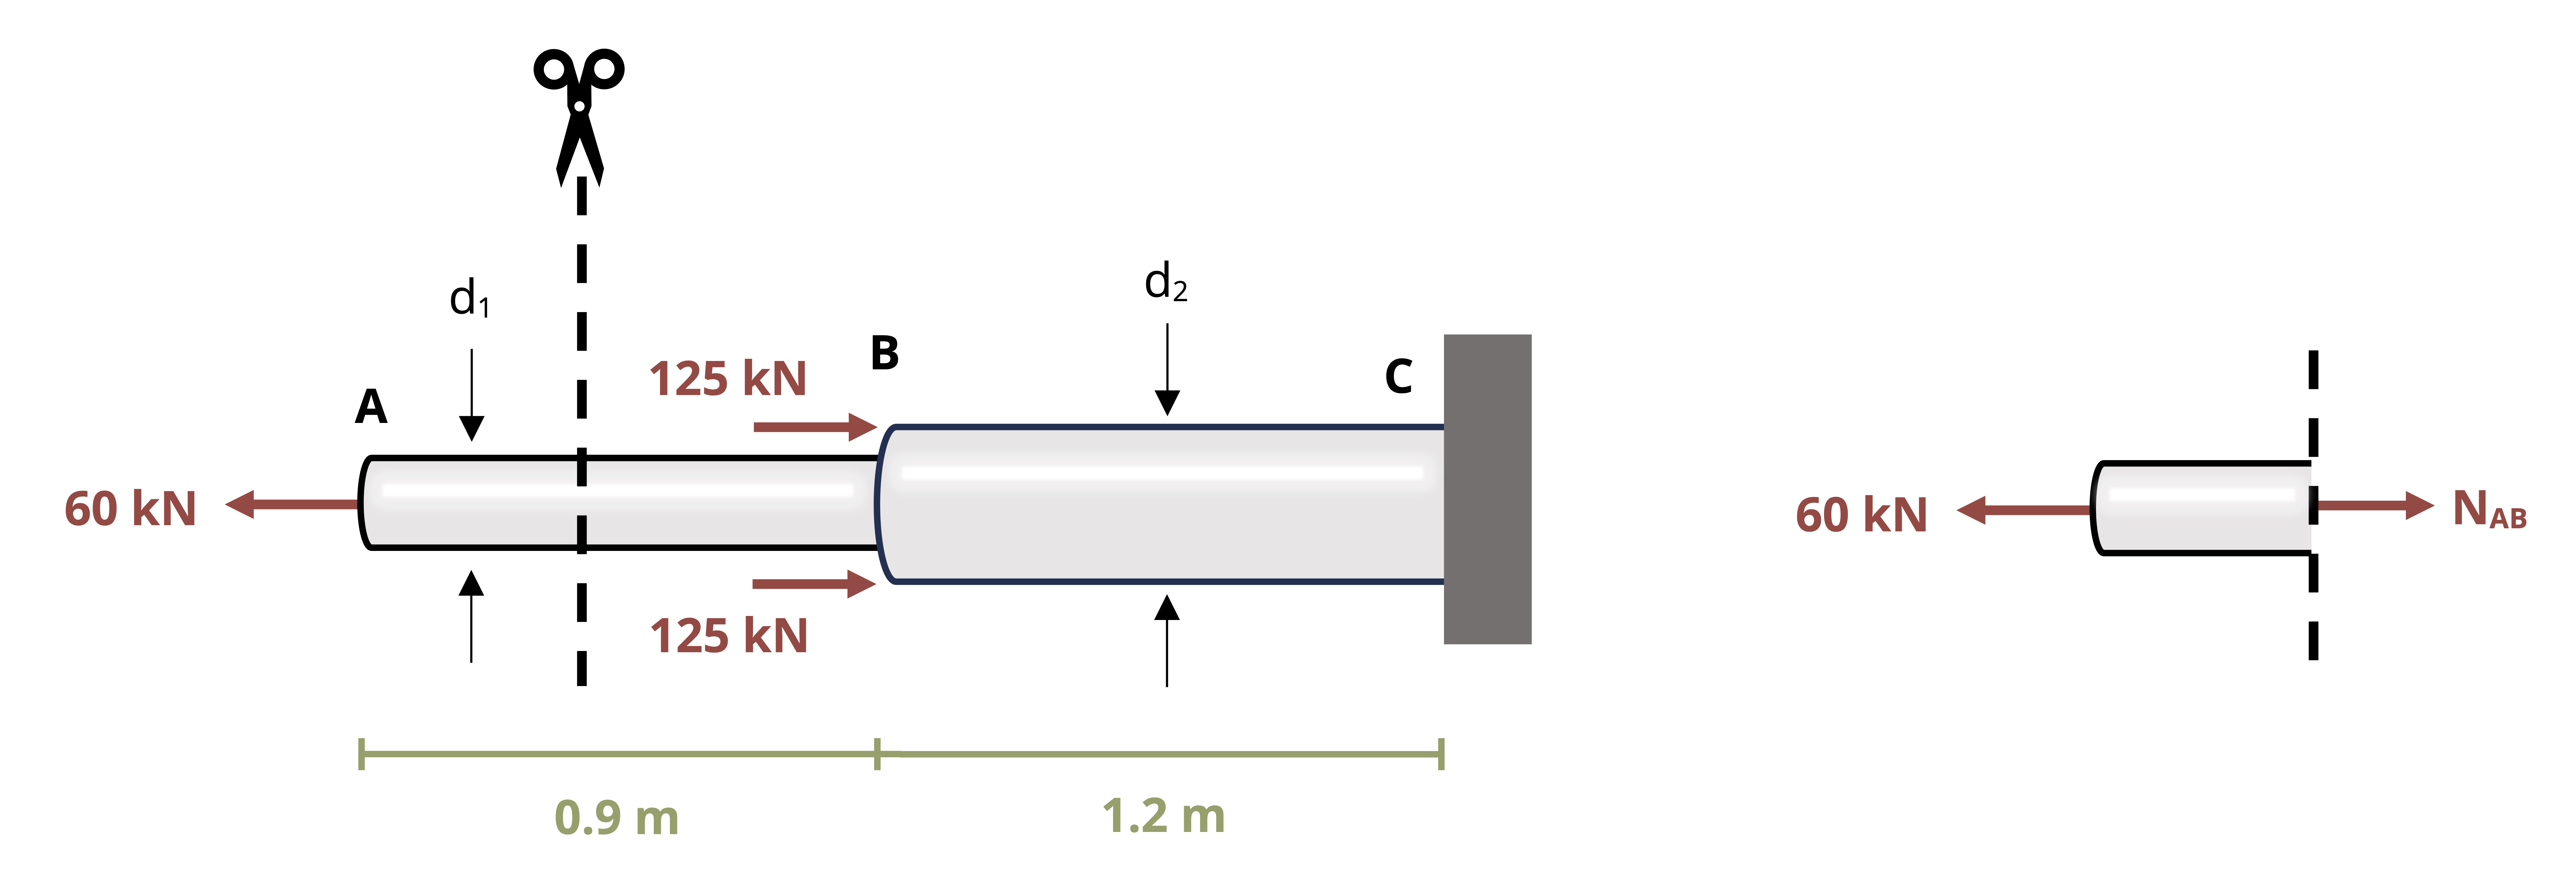
\includegraphics{images/CH1 PNGs/example 1.5 part 2.png}
\end{center}

\[
\sum F_x=-60 k N+N_{A B}=0 \rightarrow N_{A B}=60 \text{ kN}
\]

Making the cut in section BC and drawing the FBD allows us to determine
the normal force in section BC. Once again, drawing the left section of
the cut for the FBD results in avoiding needing to know the external
reactions at wall C.

\begin{center}
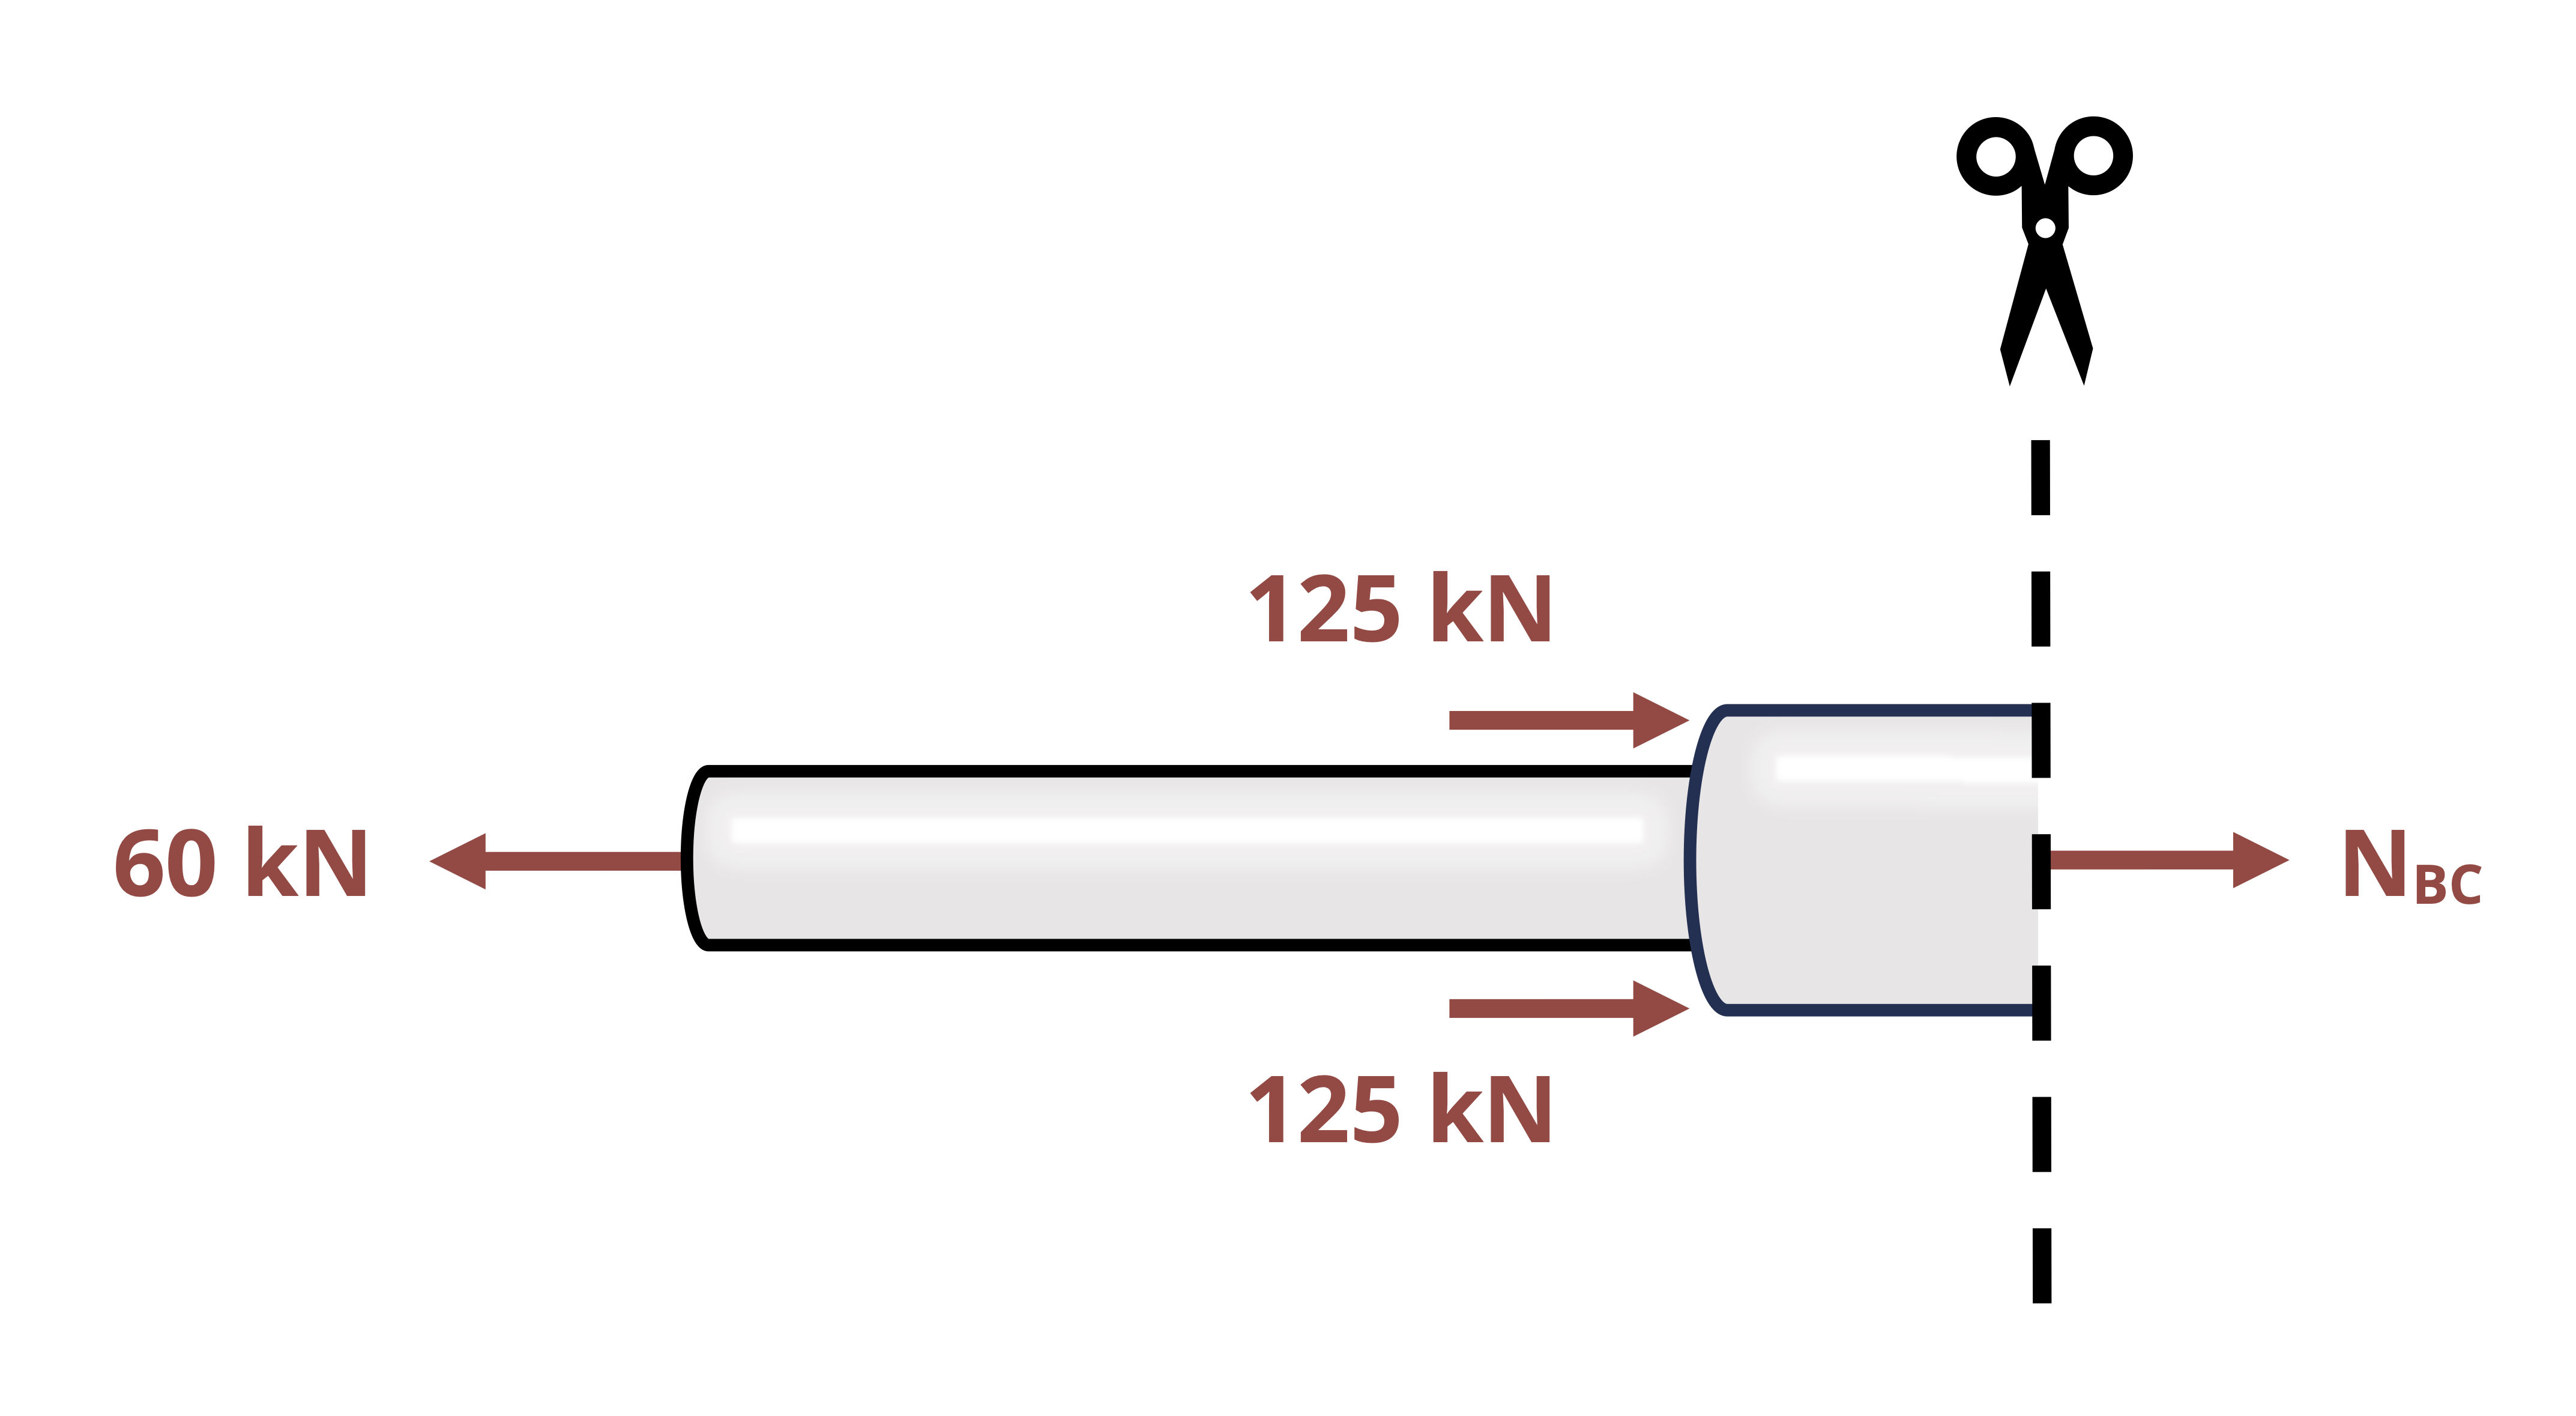
\includegraphics[width=3.5625in,height=\textheight]{images/CH1 PNGs/example 1.5 part 3.png}
\end{center}

\[
\sum F_x=-60 k N+250 k N+N_{B C}=0 \rightarrow N_{B C}=-190 \text{ kN}
\]

For both AB and BC, the internal normal force was assumed tensile in the
FBD and equilibrium equation. In the case of NAB, the positive answer
confirms that it is tensile. In the case of NBC, the negative answer
reveals that it is compressive.

\begin{center}
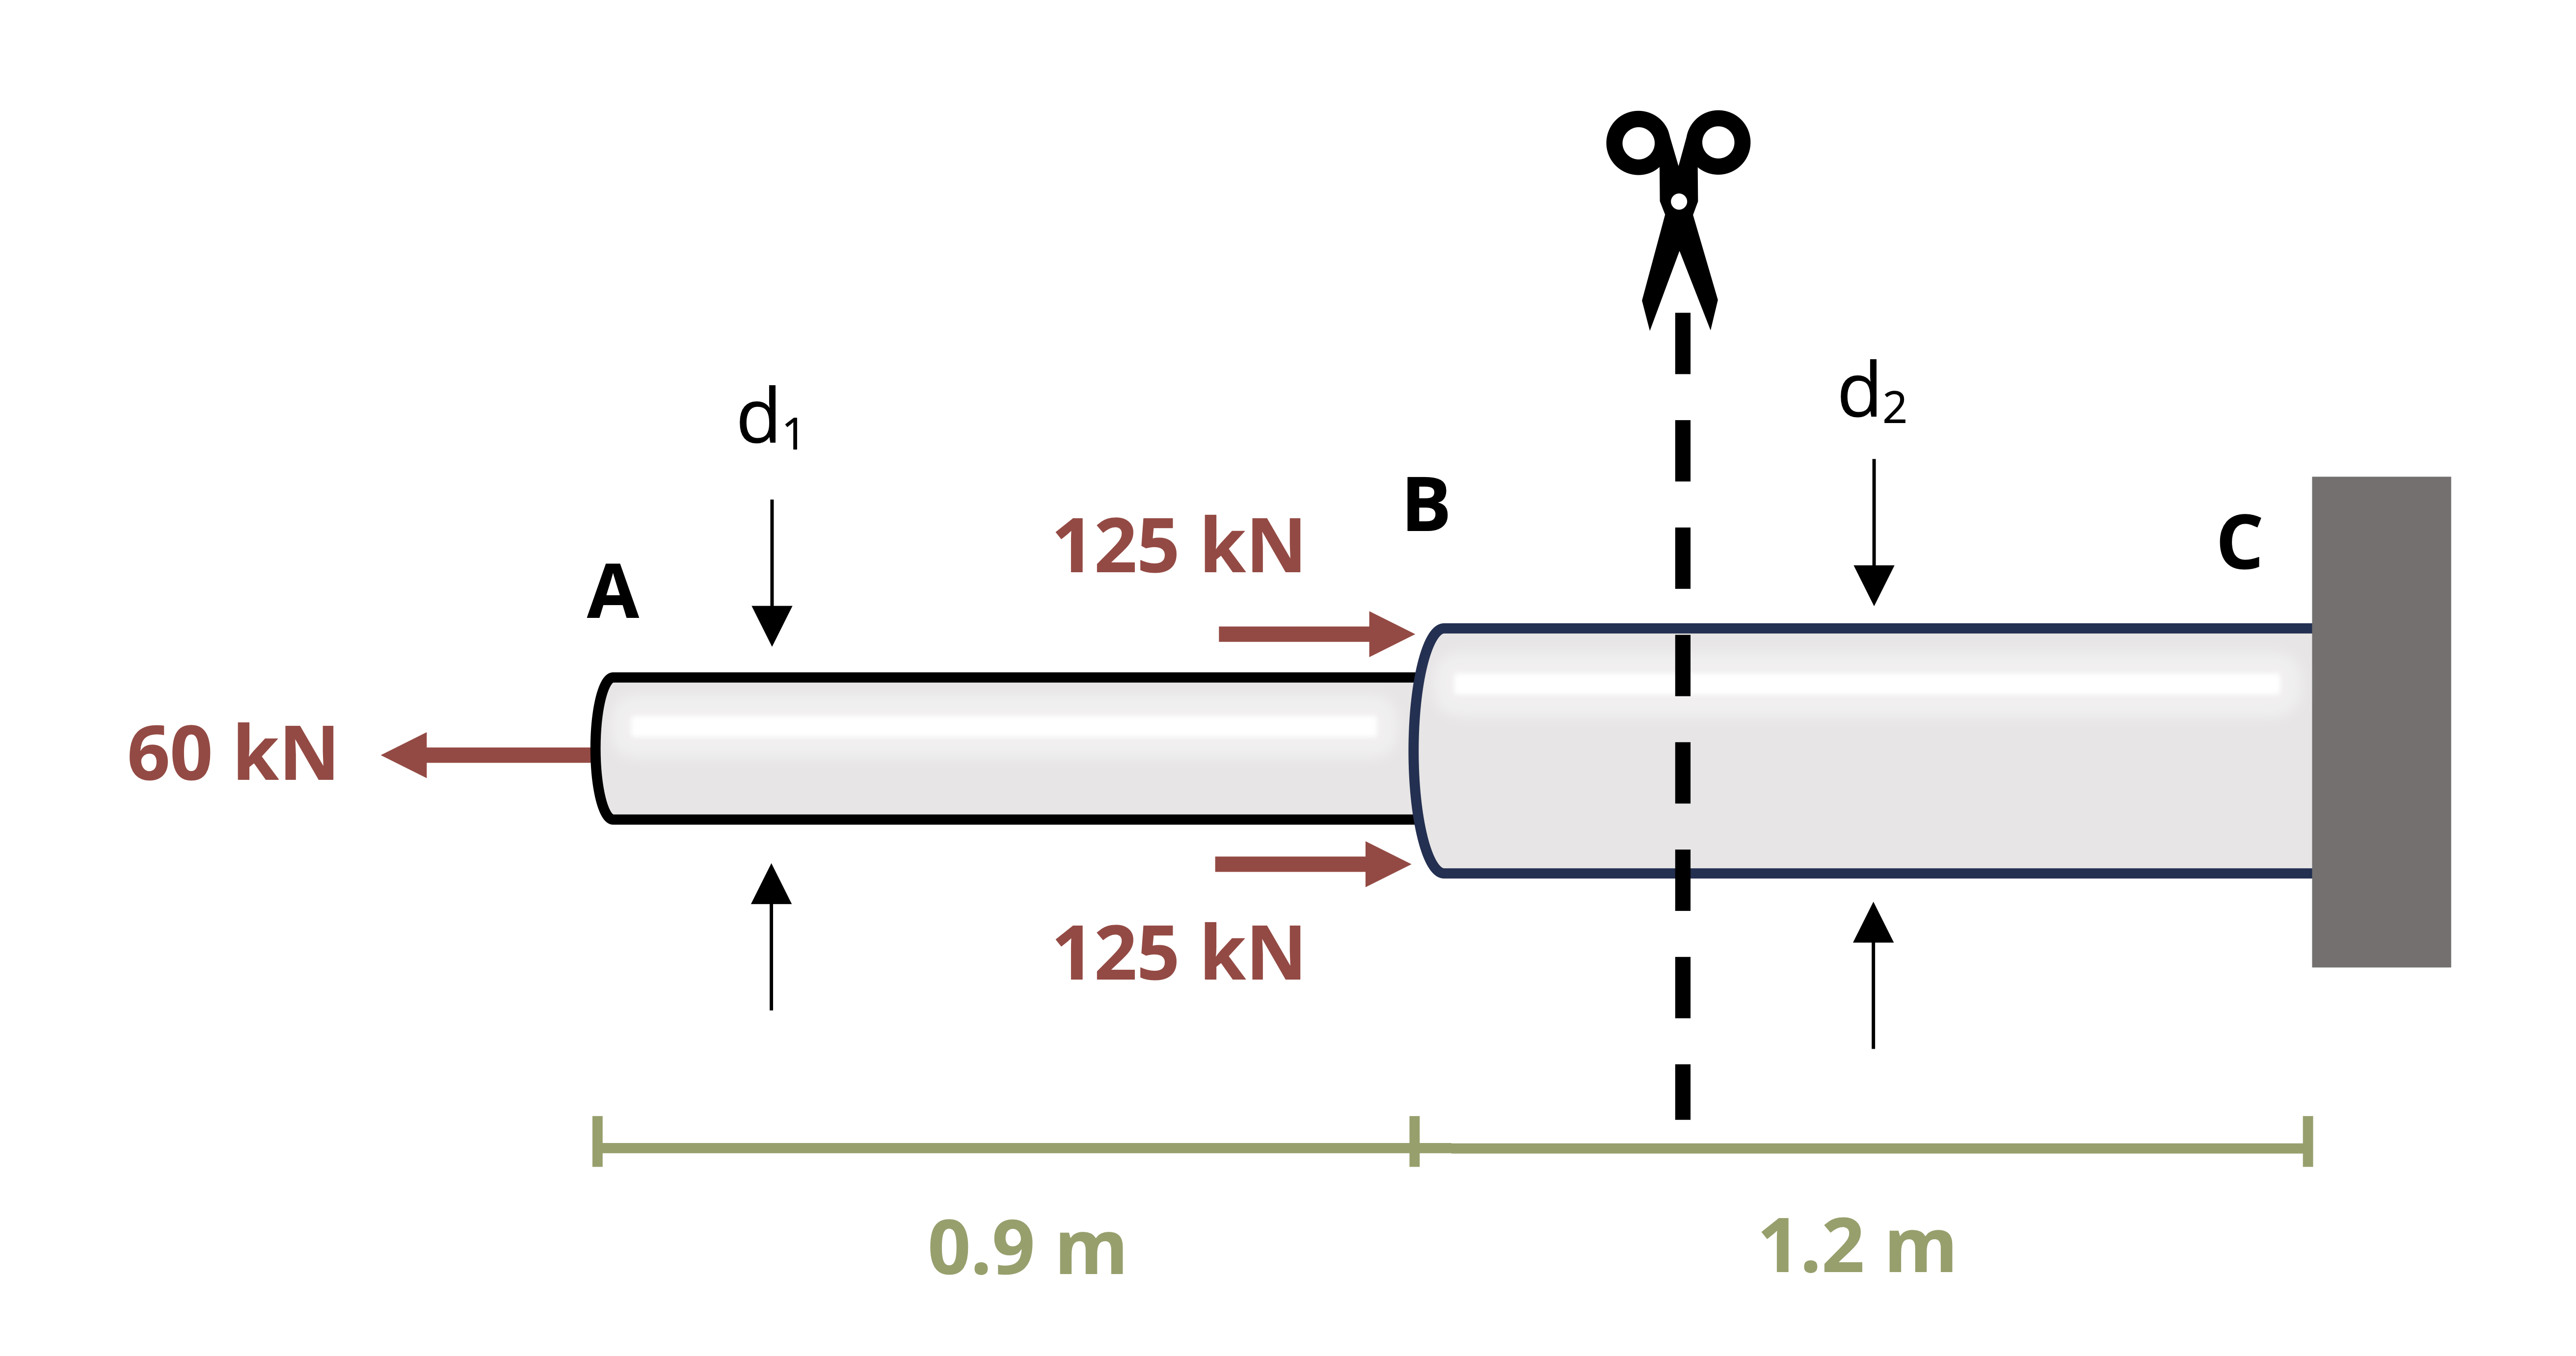
\includegraphics[width=4.34375in,height=\textheight]{images/CH1 PNGs/example 1.5 part 4.png}
\end{center}

\textbf{Answer: NAB = 60 kN (T), NBC = 190 kN (C)}

\end{tcolorbox}

\section{Equilibrium and Reactions in Three
Dimensions}\label{equilibrium-and-reactions-in-three-dimensions}

Click to expand

Because real life structures will be subject to forces and moments in
all directions, we will also see problems in which it will be necessary
to consider 3 dimensional forces and 3 dimensional moments.

For 3D systems, there are 6 total scalar equilibrium equations:

\[
\begin{array}{ll}
\sum F_x=0 & \sum M_x=0 \\
\sum F_y=0 & \sum M_y=0 \\
\sum F_z=0 & \sum M_z=0
\end{array}
\]

Note that the moment vector describes the axis around which the body
tends to rotate. Each individual component represents the tendency of
the body to rotate around the specified axis. In 3D, there are three
internal forces and three internal moments (Figure 1.3). There is one
normal force (N\textsubscript{x}) perpendicular to the cross-section and
two shear forces (V\textsubscript{y} and V\textsubscript{z}) parallel to
the cross-section. There are two bending moments (M\textsubscript{y} and
M\textsubscript{z}) which act around the axes parallel to the
cross-section and one torsional moment (T\textsubscript{x}) which acts
around the axis perpendicular to the cross-section. We will study each
of these loads in detail over the next few chapters.

\begin{figure}[H]

{\centering 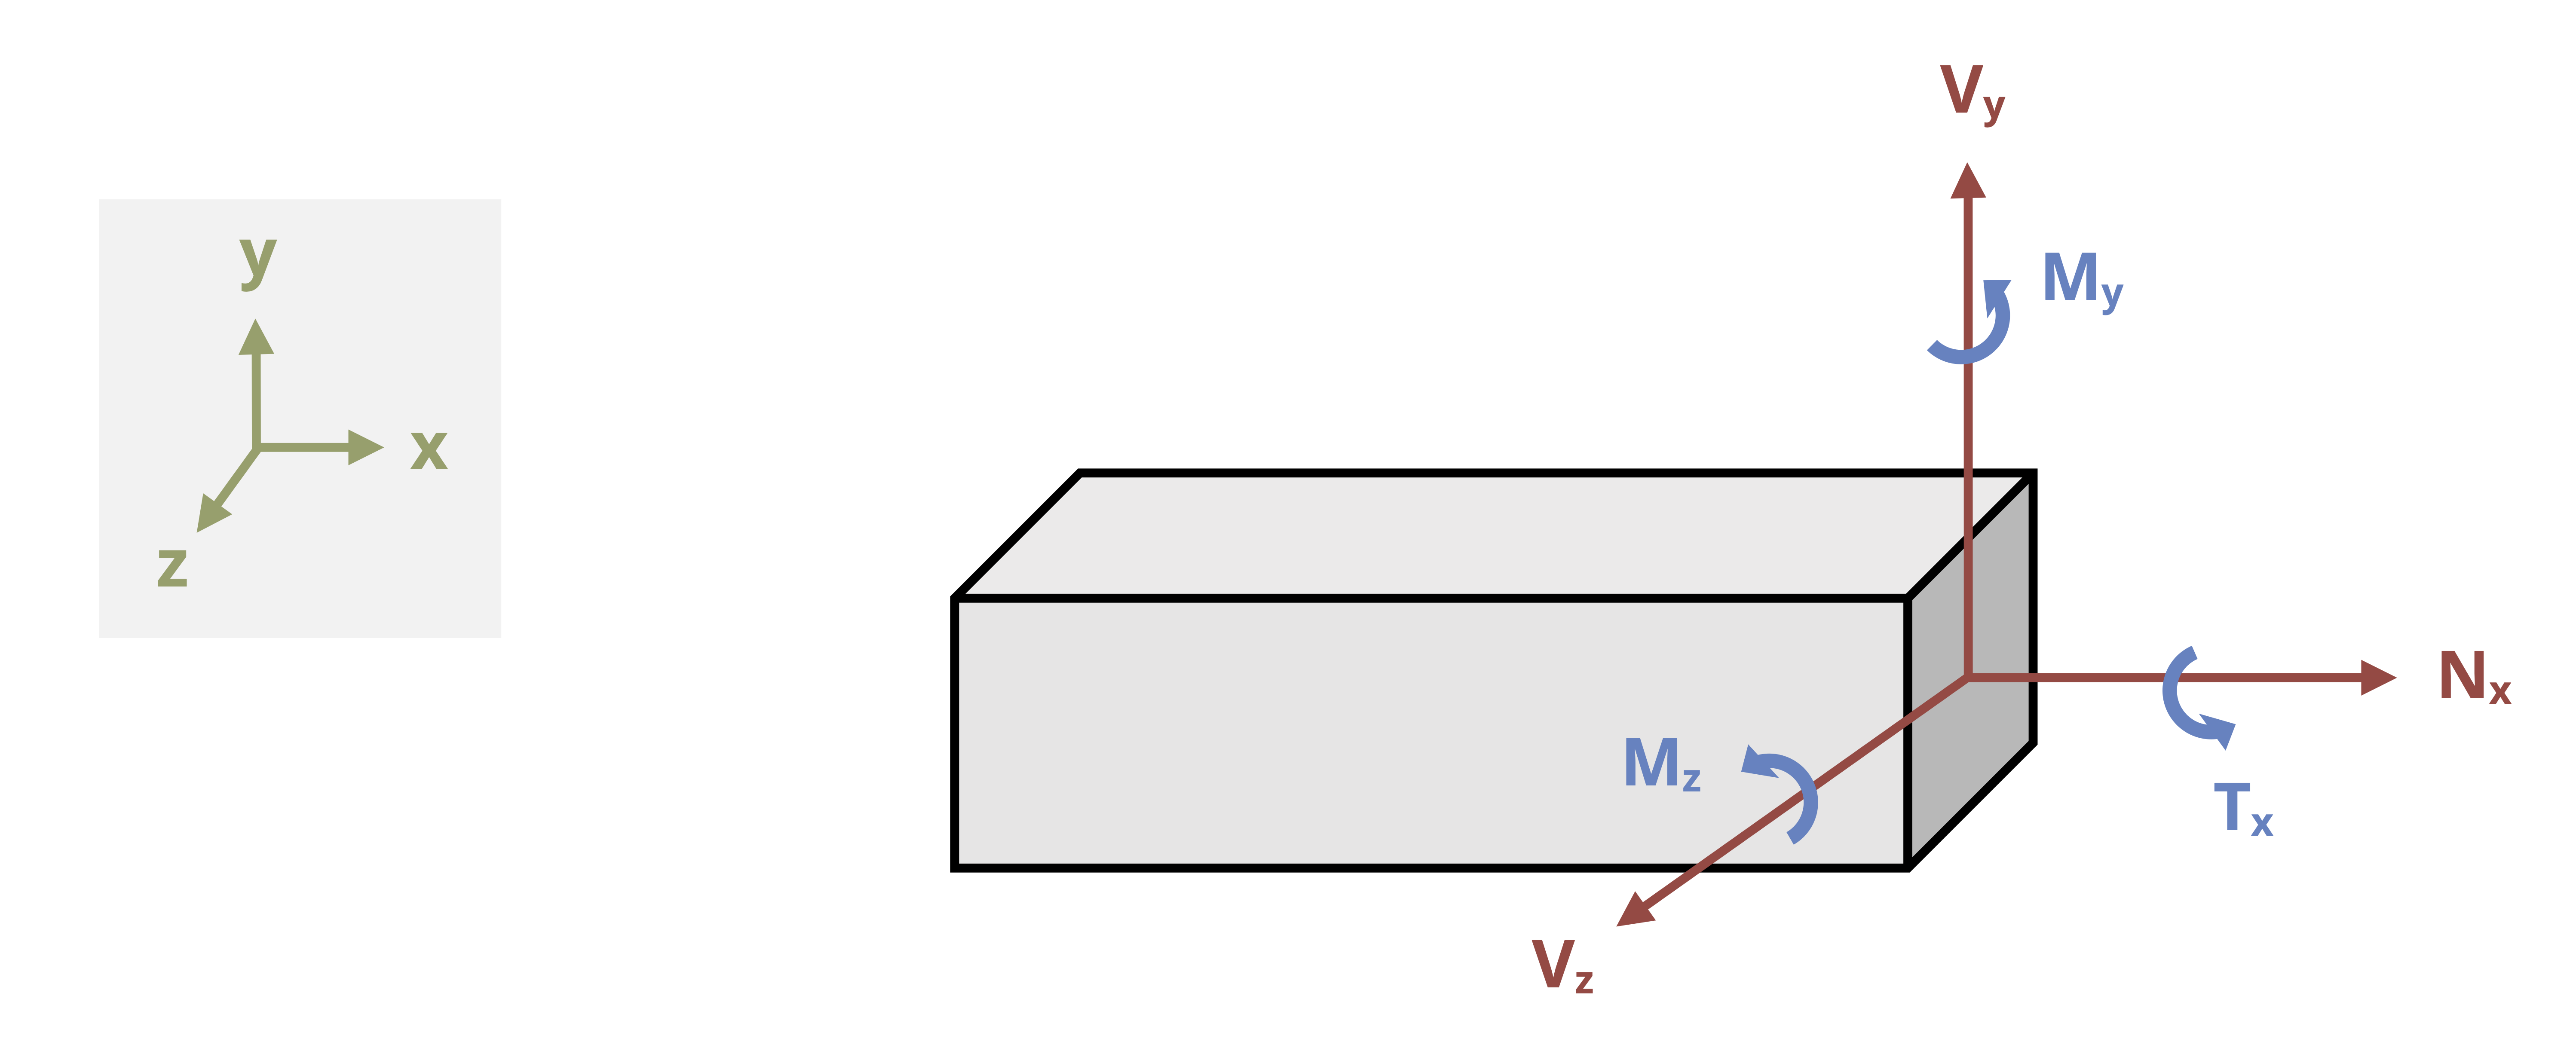
\includegraphics[width=5.3125in,height=\textheight]{images/CH1 PNGs/figure 1.3.png}

}

\caption{Figure 1.3: In 3D there are three internal forces (normal force
N\textsubscript{x} and two shear forces V\textsubscript{y} and
V\textsubscript{z}) and three internal moments (torsional moment
T\textsubscript{x} and two bending moments M\textsubscript{y} and
M\textsubscript{z})}

\end{figure}%

Note that the choice of coordinate system here is arbitrary. Loads are
defined as normal, shear, bending, or torsion based on how they act
relative to the cross-section. For example, the normal force may act in
the y-direction depending on how the cross-section is cut, and the
torsional moment would then act around the y-axis.

While summing the reaction forces in 3D is a straight-forward process of
adding forces in each direction, summing moments in 3D can prove to be
more complicated. To sum moments, there are generally two options. One
option is to use the cross product to calculate moments:
\(M=r \times F\)

In the cross-product equation, \textbf{r} is the position vector from
the point the moment is about to any point on the line of action of the
force. Using the cross product to calculate moment will result in a
vector expression for the moment equation that gives all three
components at one time with the correct signs to indicate clockwise
(negative) or counterclockwise (positive) rotation.

The second option to calculate moments is to perform scalar calculations
in which the sum of the moments about the x, y, and z axis is calculated
individually. To use this option, it might be helpful to recall:

\begin{enumerate}
\def\labelenumi{\arabic{enumi}.}
\item
  The general scalar equation for moment is M = F*d, where d is the
  perpendicular distance from the axis of rotation at the point the
  moment is being taken about to anywhere on the line of action of the
  force. One can also use M = F r sin α where r is the distance from the
  point to any point on the force and α is the angle between the
  position vector \textbf{r} (that corresponds to the magnitude r used)
  and the force vector.
\item
  Forces do not cause moments about points they go through or axes they
  act through.
\item
  Forces do not cause moments about axes they are parallel to (i.e.,
  F\textsubscript{x} wouldn't cause a moment around an x-axis no matter
  where the point is).
\item
  When taking the moment about a point, the origin of the coordinate
  axes should be moved to that point for the purpose of determining the
  distance between the axis and the force.
\end{enumerate}

Given all the reminders above, one can apply the following equations:

\(\sum M_x= \pm F_y * z \pm F_z * y\) where z and y are the respective
distances from the x-axis at the point in question to F\textsubscript{y}
and F\textsubscript{z} components of the force respectively.

\(\sum M_y= \pm F_x * z \pm F_z * x\) where z and x are the respective
distances from the y-axis at the point in question to F\textsubscript{x}
and F\textsubscript{z} components of the force respectively.

\(\sum M_z= \pm F_x * y \pm F_y * x\) where y and x are the respective
distances from the z-axis at the point in question to the
F\textsubscript{x} and F\textsubscript{y} components of the force
respectively.

The ± is decided based on the right-hand rule (see text below for
guidance) or visual inspection. When using visual inspection, the
direction of rotation is judged by looking from the positive end of the
axis towards the negative end. A counterclockwise rotation is considered
to be positive and a clockwise rotation is considered to be negative.

To apply the right-hand rule:

\begin{enumerate}
\def\labelenumi{\arabic{enumi}.}
\item
  Orient your right hand so that the fingers are aligned with the moment
  arm with the palm at the point and the fingertips extending towards
  the force. The moment arm is the axis along which the perpendicular
  distance to the axis would be determined. For example, if finding
  M\textsubscript{x} due to F\textsubscript{y}, the moment arm is in the
  z direction.
\item
  The thumb is aligned with the axis of rotation (axis around which the
  moment is being calculated).
\item
  Curl your fingers in the direction of the force. If your thumb must be
  pointed in the positive axis direction to perform this action, the
  moment is counterclockwise. If your thumb must be pointed in the
  negative axis direction, the moment is clockwise. Typical convention
  designates counterclockwise rotation to be positive and clockwise to
  be negative.
\end{enumerate}

These concepts are further reviewed in Example 1.6.

\begin{tcolorbox}[enhanced jigsaw, colback=white, colframe=quarto-callout-note-color-frame, leftrule=.75mm, opacitybacktitle=0.6, colbacktitle=quarto-callout-note-color!10!white, arc=.35mm, bottomrule=.15mm, breakable, title={Example 1.6}, left=2mm, titlerule=0mm, toptitle=1mm, toprule=.15mm, opacityback=0, rightrule=.15mm, coltitle=black, bottomtitle=1mm]

Determine the internal reactions at point P, located at the center of
the cross-section of the rectangular bar and 1.75 ft from the fixed
support, if \textbf{F} = -150 \textbf{i} - 225 \textbf{j} + Fz = 300
\textbf{k} lb.

\begin{center}
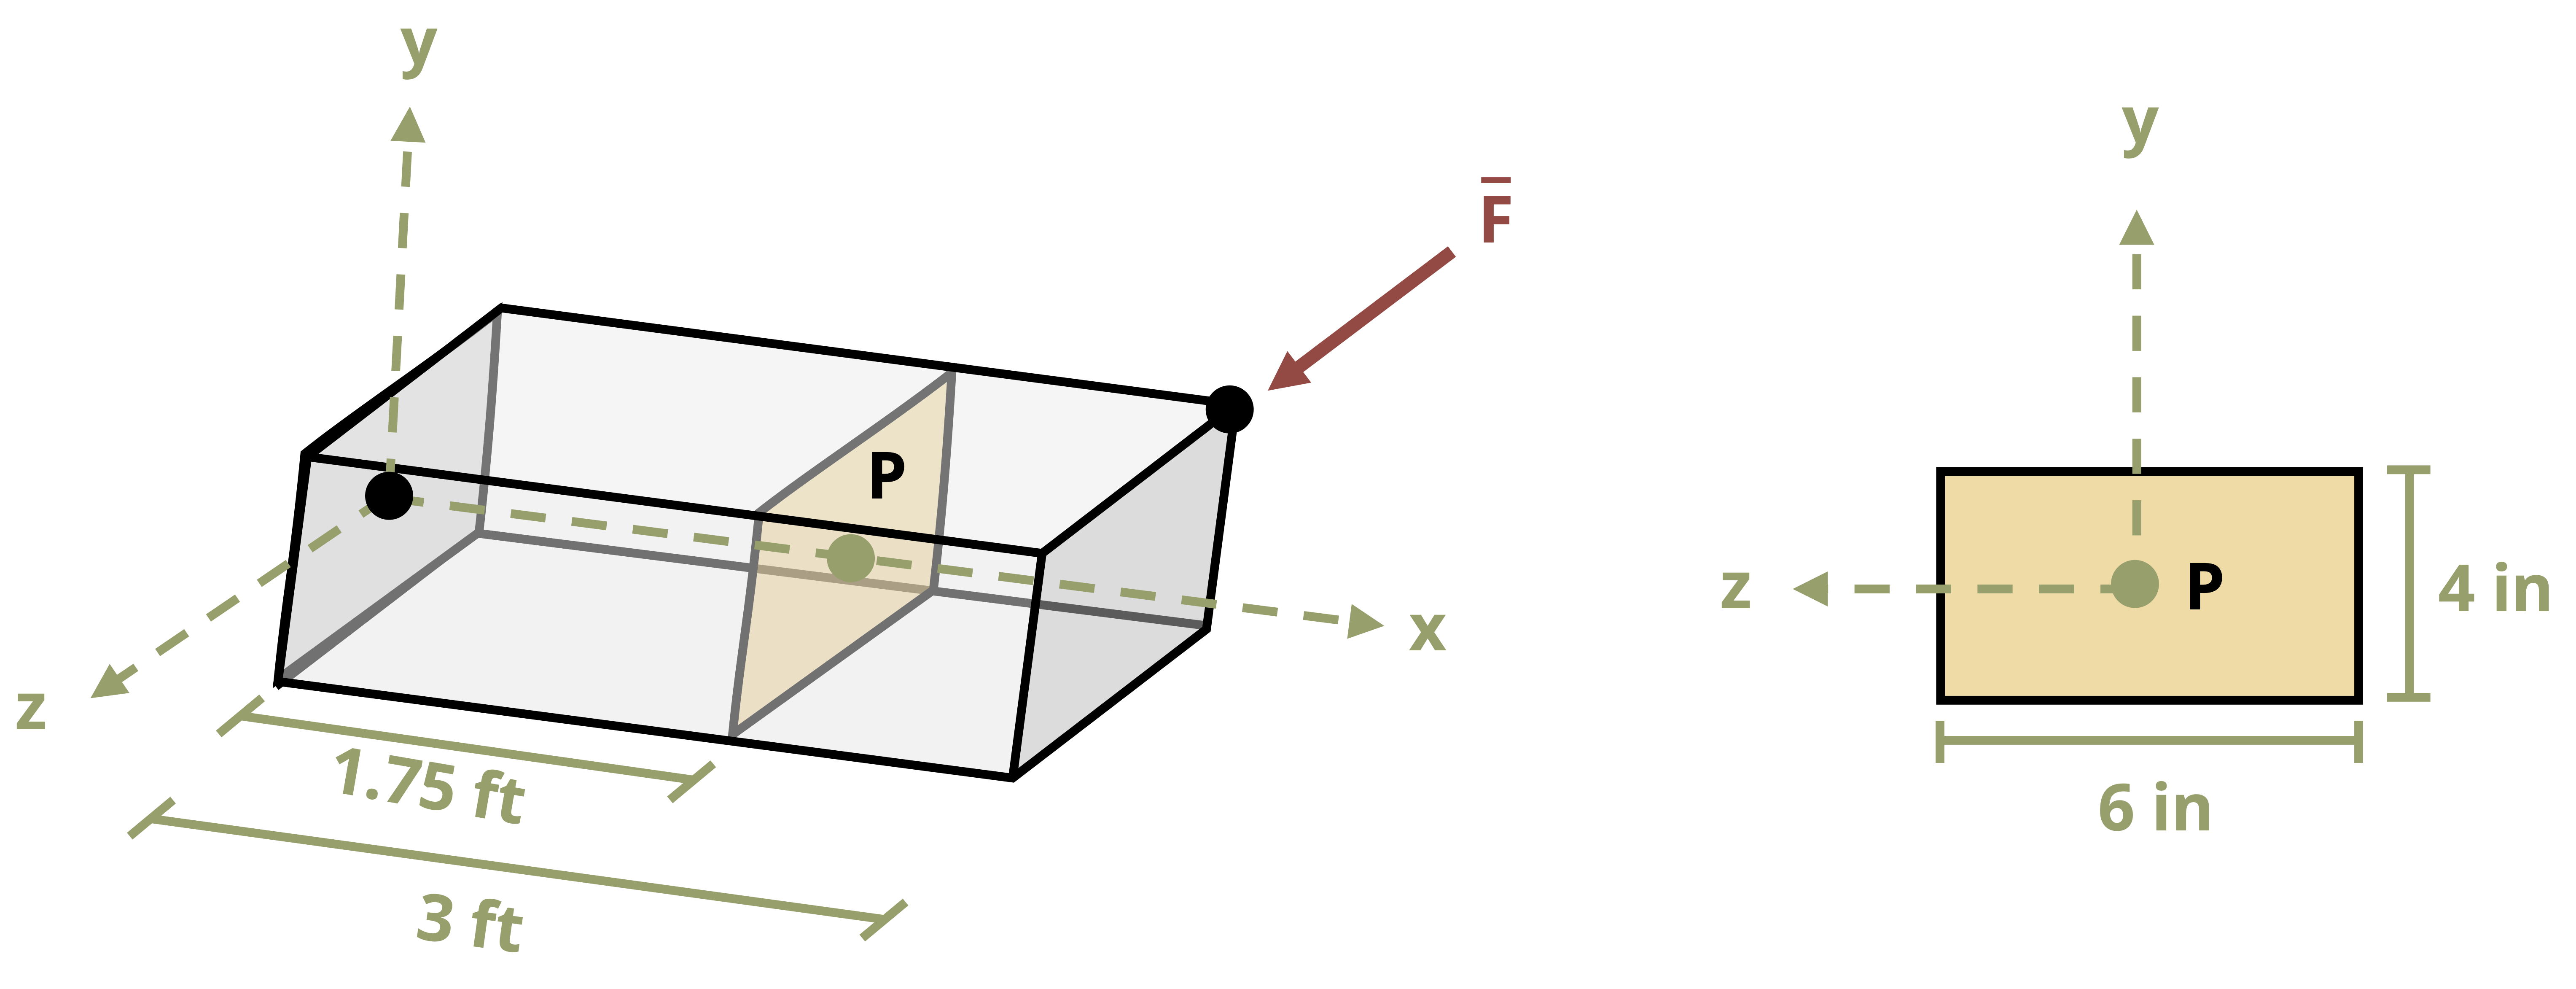
\includegraphics[width=5.04167in,height=\textheight]{images/CH1 PNGs/example 1.6 part 1.png}
\end{center}

To determine the internal reactions at P, a cut is made at P that is
parallel to the cross section. Since the left side of the cut would
include the wall but the right side of the cut would be free with no
external reactions to determine, the right side section will be used.

\begin{center}
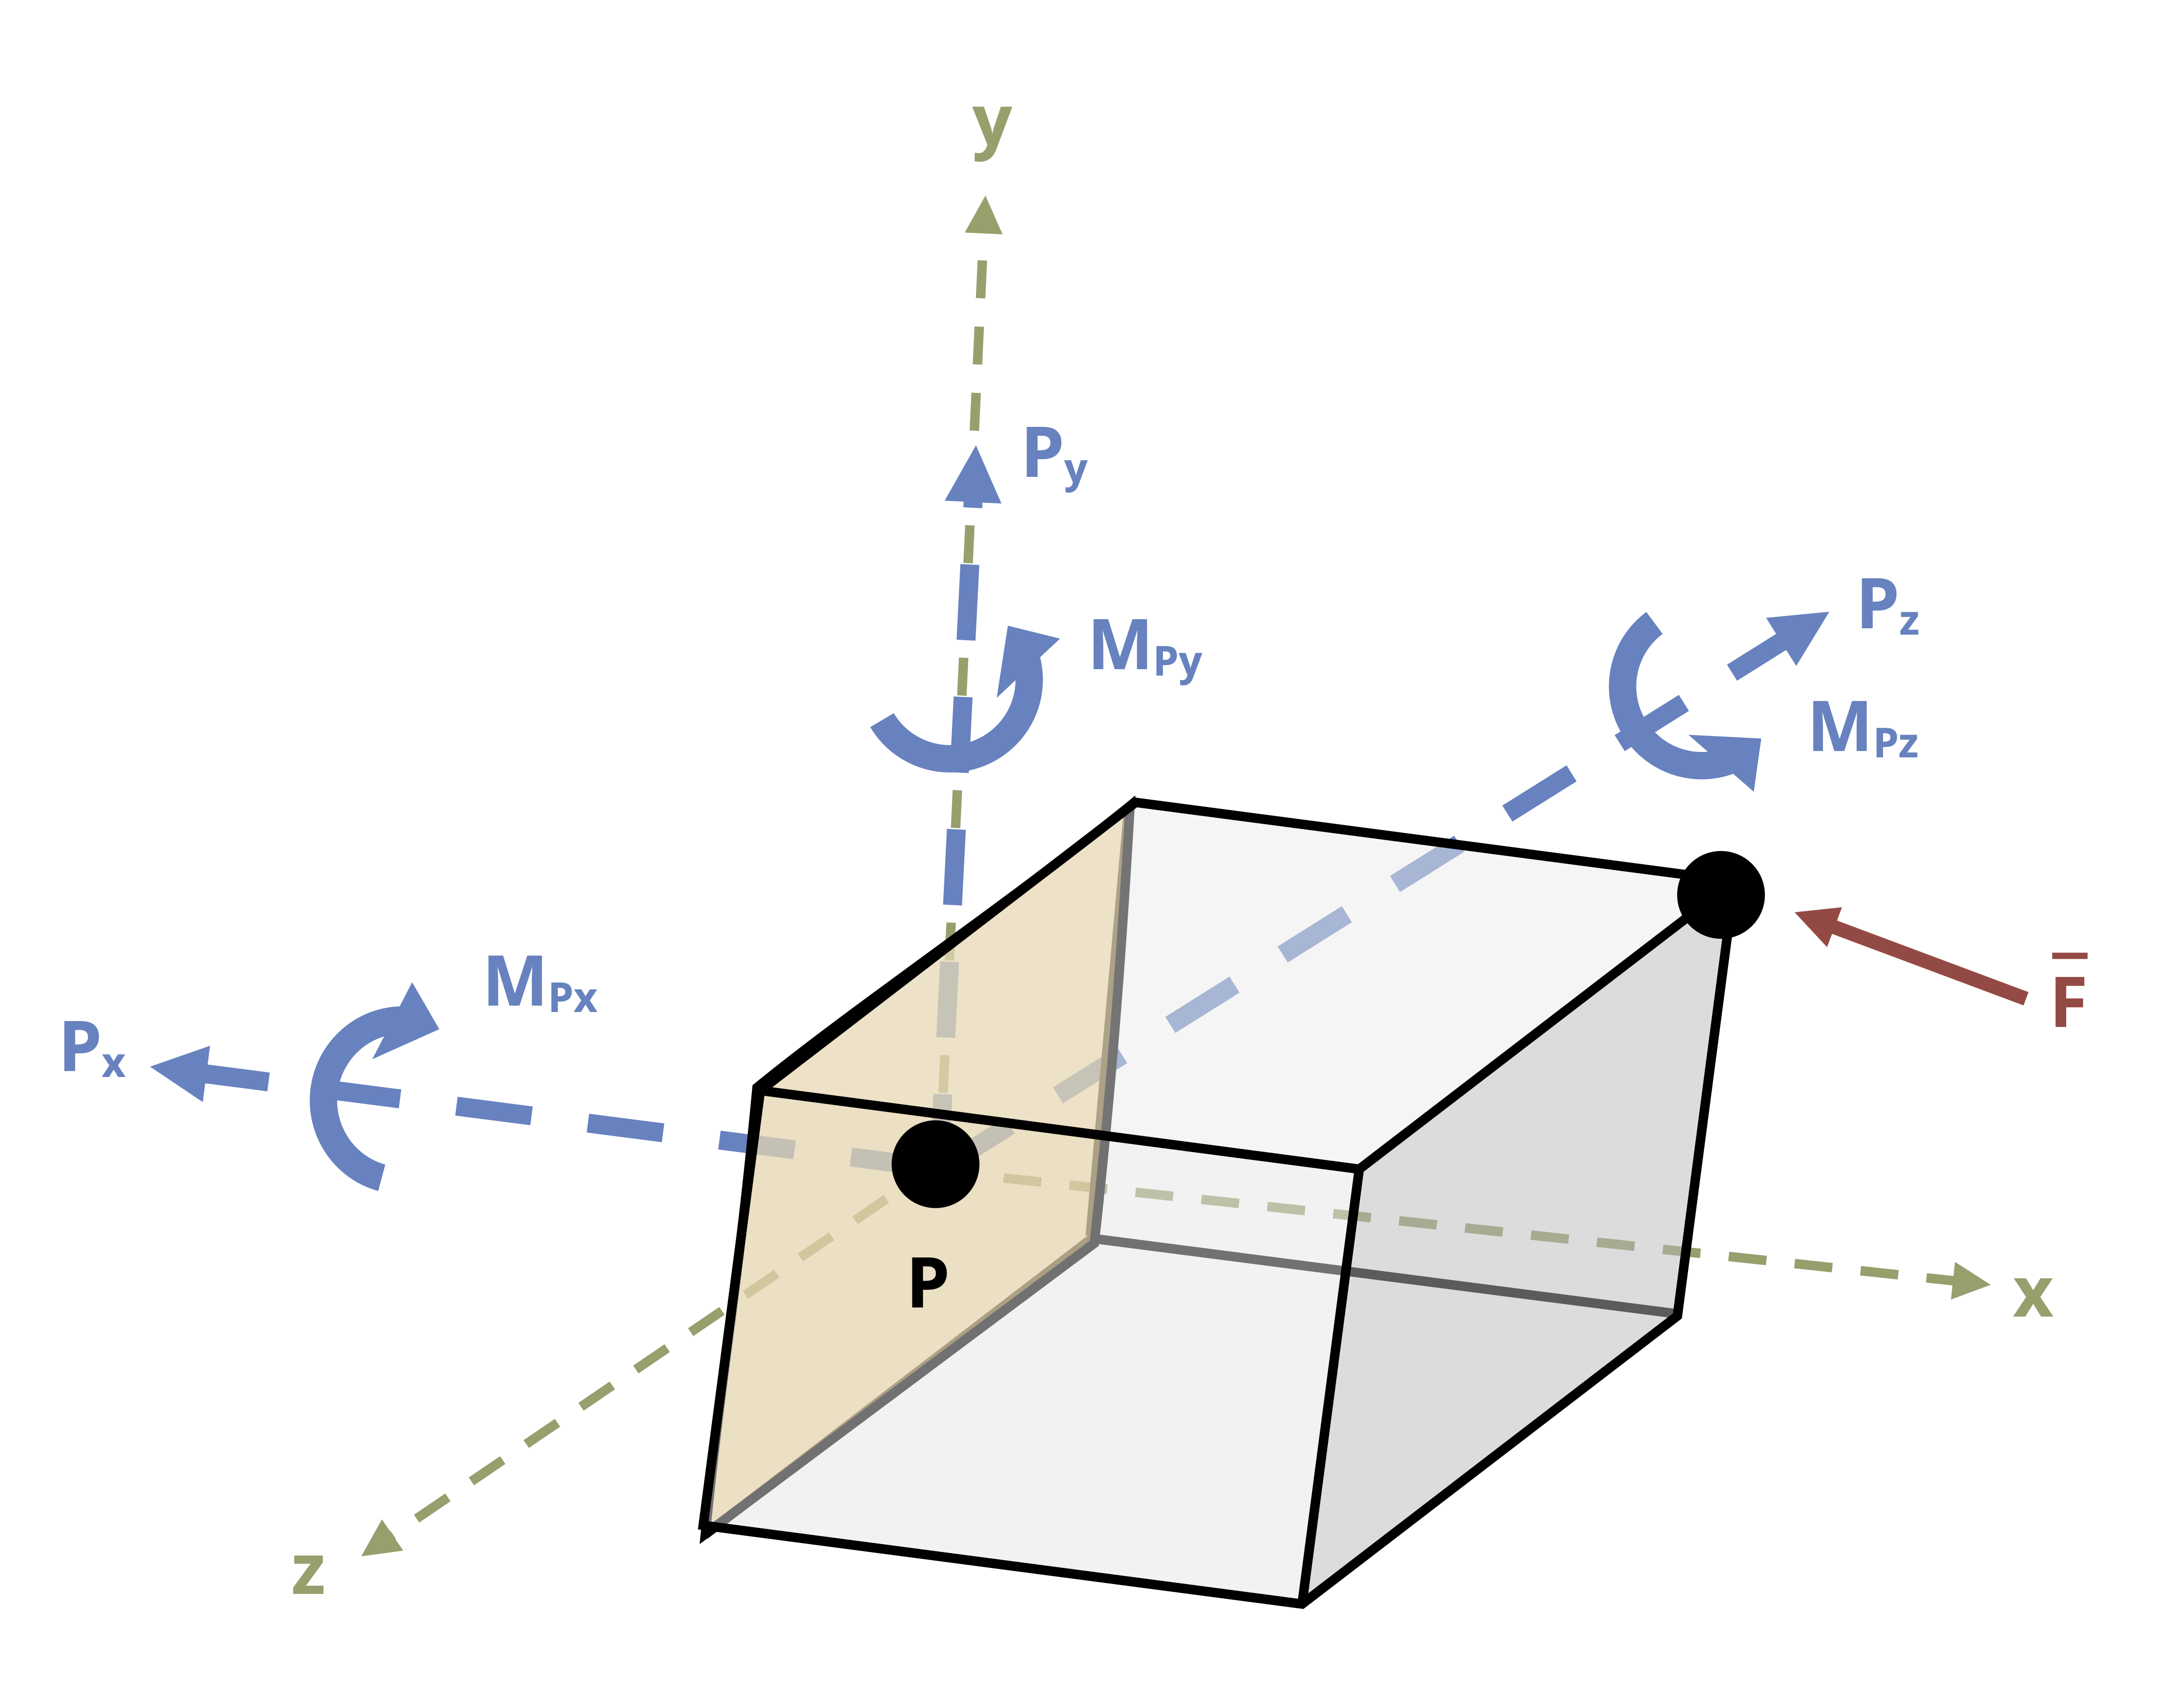
\includegraphics[width=4.04167in,height=\textheight]{images/CH1 PNGs/example 1.6 part 2.png}
\end{center}

The force reactions at P will just be equal (but opposite in direction)
to the force shown since there is only one. The moment reactions can be
found by taking the moments about point P.

The moment about the x axis at point P is:

\[
\sum M_{Px} = \pm F_yz \pm F_zy = 0 = -[(225 \text{ lb})(3 \text{ in})(\frac{1 \text{ ft}}{12 \text{ in}})]+[(300 \text{ lb})(2 \text{ in})(\frac{1 \text{ ft}}{12 \text{ in}})]+M_{px} -6.25 \text{ lb ft}
\]

The moment about the y axis at point P is:

\[
\sum M_{Py} = \pm F_xz \pm F_zx = 0 = -[(150 \text{ lb})(3 \text{ in})(\frac{1 \text{ ft}}{12 \text{ in}})]-[(300 \text{ lb})(1.25 \text{ ft})]+M_{py} -347.5 \text{ lb ft}
\]

The moment about the z axis at point P is:

\[
\sum M_{Pz} = \pm F_xy \pm F_yx = 0 = [(150 \text{ lb})(2 \text{ in})(\frac{1 \text{ ft}}{12 \text{ in}})]-[(225 \text{ lb})(1.25 \text{ ft})]+M_{pz} -2.5 \text{ lb ft}
\]

The sign on the individual multiplicative terms in each equation are
determined by right hand rule or visualization.

\textbf{Answer:}

P\textsubscript{x} = 150 lb

P\textsubscript{y} = 225 lb

P\textsubscript{z} = 300 lb

M\textsubscript{Px} = 6.25 lb ft

M\textsubscript{Py} = 348 lb ft

M\textsubscript{Pz} = 2.5 lb ft

\end{tcolorbox}

\section*{Summary}\label{summary}
\addcontentsline{toc}{section}{Summary}

\markright{Summary}

Click to expand

\begin{tcolorbox}[enhanced jigsaw, colback=white, colframe=quarto-callout-note-color-frame, leftrule=.75mm, opacitybacktitle=0.6, colbacktitle=quarto-callout-note-color!10!white, arc=.35mm, bottomrule=.15mm, breakable, title={Key takeaways}, left=2mm, titlerule=0mm, toptitle=1mm, toprule=.15mm, opacityback=0, rightrule=.15mm, coltitle=black, bottomtitle=1mm]

Bodies in this text are in static equilibrium and subjected to external
forces and moments. Reaction forces and moments at supports can be
determined in 2D and 3D through equilibrium equations, just like in
Statics.

Unlike Statics, bodies in this course are deformable. We must also
determine internal loads. These can be found by cutting a cross-section
at the point of interest and again applying equilibrium equations.

In 2D there are two internal forces and one internal moment:

\begin{itemize}
\item
  Normal force (N) perpendicular to the cross-section
\item
  Shear force (V) parallel to the cross-section
\item
  Bending moment (M)
\end{itemize}

In 3D there are three internal forces and three internal moments:

\begin{itemize}
\item
  Normal force (N) perpendicular to the cross-section
\item
  Two shear forces (V) parallel to the cross-section
\item
  Torsional moment (T) acting around the axis perpendicular to the
  cross-section
\item
  Two bending moments (M) acting around the axes parallel to the
  cross-section
\end{itemize}

The effects of these internal loads on deformable bodies is the focus of
this text.

\end{tcolorbox}

\begin{tcolorbox}[enhanced jigsaw, colback=white, colframe=quarto-callout-note-color-frame, leftrule=.75mm, opacitybacktitle=0.6, colbacktitle=quarto-callout-note-color!10!white, arc=.35mm, bottomrule=.15mm, breakable, title={Key equations}, left=2mm, titlerule=0mm, toptitle=1mm, toprule=.15mm, opacityback=0, rightrule=.15mm, coltitle=black, bottomtitle=1mm]

Static equilibrium:

\[
\begin{array}{ll}
\sum F_x=0 & \sum M_x=0 \\
\sum F_y=0 & \sum M_y=0 \\
\sum F_z=0 & \sum M_z=0
\end{array}
\]

\end{tcolorbox}

\bookmarksetup{startatroot}

\chapter{Stress}\label{sec-stress}

\begin{tcolorbox}[enhanced jigsaw, colback=white, colframe=quarto-callout-note-color-frame, leftrule=.75mm, opacitybacktitle=0.6, colbacktitle=quarto-callout-note-color!10!white, arc=.35mm, bottomrule=.15mm, breakable, title={Learning Objectives}, left=2mm, titlerule=0mm, toptitle=1mm, toprule=.15mm, opacityback=0, rightrule=.15mm, coltitle=black, bottomtitle=1mm]

\begin{itemize}
\tightlist
\item
  Use internal loads to calculate average normal stress
\item
  Use internal loads to calculate average shear stress
\item
  Use the loads between surfaces to calculate bearing stress
\item
  Calculate stresses on inclined planes
\end{itemize}

\end{tcolorbox}

\section{Introduction}\label{introduction-2}

Click to expand

Having reviewed static equilibrium in Chapter 1, we now know how to find
the internal loads in a body using equilibrium. When determining whether
a body can resist the loads applied to it, the internal load is only
part of the solution. The dimensions of the body and the inherent
properties of the material it is made from are also important.

In this chapter we'll explore the concept of stress, which can help us
determine whether an object will physically break when subjected to a
load. We'll cover average normal stress (stress perpendicular to the
cross-section) in Section 2.1 and average shear stress (stress parallel
to the cross-section) in Section 2.2. We'll then discuss bearing stress
(the stress between two bodies in contact with each other) in Section
2.3 and finish with the average normal and shear stresses on an inclined
cross-section in Section 2.4.

\section{Average Normal Stress}\label{average-normal-stress}

Click to expand

Average normal stress is defined as the internal normal force divided by
the cross-sectional area of the body. It is given the Greek letter sigma
(σ). Stress increases as the force increases or as the cross-sectional
area decreases.

{[}math{]}

\emph{where}

\emph{𝜎 = Average normal stress {[}Pa, psi{]}}

\emph{N = Internal normal force {[}N, lb{]}}

\emph{A = Cross-sectional area {[}m\textsuperscript{2},
in\textsuperscript{2}{]}}

As such the SI units of stress are N/m\textsuperscript{2}, more commonly
referred to as the Pascal (Pa) where 1 Pa = 1 N/m\textsuperscript{2}.
The US customary units for stress are lb/in.2, commonly written as psi.
Since stresses can get very large, it is common to use prefixes such as
kilo (k) and mega (M) to represent 10\textsuperscript{3} and
10\textsuperscript{6} respectively. A stress of 15,000,000 Pa is written
as 15 MPa. A stress of 35,000 psi is written as 35 ksi.

Normal stress occurs perpendicular to the cross-section and so is
associated with either a pulling or pushing motion (Figure 2.1). Normal
forces that pull on a cross-section are known as tensile forces and
create a tensile normal stress. Normal forces that push on a
cross-section are known as compressive forces and create a compressive
normal stress. The normal stress calculated above is really an average
normal stress as the force is distributed over the cross-section, but we
generally simplify this to a concentrated force that creates the same
normal stress at every point on the cross-section (Figure 2.2).

\textbf{Figure 2.1:} Forces pulling on a cross-section cause tension,
while forces pushing on a cross-section cause compression. Both are very
common. (Left) A crane cable during a lift experiences tension. (Right)
The support columns under a bridge experience compression.

\textbf{Figure 2.2:} The internal load is equally distributed over the
cross-sectional area, but may be represented as a single concentrated
load acting at the center (N in this case). The stress is therefore an
average normal stress.

The internal normal force in a body can be found through the method of
equilibrium as learned in Statics. See Example 2.1 for a demonstration.

\begin{tcolorbox}[enhanced jigsaw, colback=white, colframe=quarto-callout-note-color-frame, leftrule=.75mm, opacitybacktitle=0.6, colbacktitle=quarto-callout-note-color!10!white, arc=.35mm, bottomrule=.15mm, breakable, title={Example 2.1: Simple normal stress}, left=2mm, titlerule=0mm, toptitle=1mm, toprule=.15mm, opacityback=0, rightrule=.15mm, coltitle=black, bottomtitle=1mm]

The support column will be subjected to a compressive force F = 65 kips.

{[}figure{]}

\begin{enumerate}
\def\labelenumi{\arabic{enumi}.}
\item
  The diameter of the column is 4 inches. Determine the average normal
  stress in the column.
\item
  The column is to be made of concrete with an allowable compressive
  stress of 4 ksi. For the same force F = 65 kips, determine the
  required diameter of the column so that the average normal stress does
  not exceed 4 ksi.
\end{enumerate}

\begin{tcolorbox}[enhanced jigsaw, colback=white, colframe=quarto-callout-note-color-frame, leftrule=.75mm, opacitybacktitle=0.6, colbacktitle=quarto-callout-note-color!10!white, arc=.35mm, bottomrule=.15mm, breakable, title={Solution}, left=2mm, titlerule=0mm, toptitle=1mm, toprule=.15mm, opacityback=0, rightrule=.15mm, coltitle=black, bottomtitle=1mm]

\begin{enumerate}
\def\labelenumi{\arabic{enumi}.}
\tightlist
\item
  Cut a cross-section through the column and draw a free body diagram.
  Although it is clear in this case that the internal load will be 65
  kips, it is best to get in the habit of writing out equilibrium
  equations.
\end{enumerate}

{[}figure{]}

{[}math{]}

The column has a circular cross-section of area {[}math{]}

The average normal stress can now be found from:

{[}math{]}

\begin{enumerate}
\def\labelenumi{\arabic{enumi}.}
\setcounter{enumi}{1}
\tightlist
\item
  Use the average normal stress equation again, but this time the stress
  is known to be 4 ksi. The loading has not changed so the internal
  normal force will still be 65 kips.
\end{enumerate}

{[}math{]}

Since {[}math{]} we can find {[}math{]}

Then {[}math{]}

Note that this is the minimum required diameter to ensure the average
normal stress does not exceed 4 ksi. If the diameter is any smaller than
this, the stress will exceed the 4 ksi limit.

\end{tcolorbox}

\end{tcolorbox}

Sometimes the loading or cross-sectional area of the body will change,
resulting in a change in stress. In these cases the stress can be
calculated separately in each segment of the body by first finding the
internal load in each segment and then dividing the internal load by the
cross-sectional area of the respective segment. Different parts of the
body may experience different stresses. Generally the highest stress is
of most importance as that is the stress that typically determines
whether the body will break. Because we do not know in advance where the
largest stress is, however, it is typically necessary to calculate the
stress at each different cross-section in order to determine the highest
stress. See Example 2.2 for a demonstration.

\begin{tcolorbox}[enhanced jigsaw, colback=white, colframe=quarto-callout-note-color-frame, leftrule=.75mm, opacitybacktitle=0.6, colbacktitle=quarto-callout-note-color!10!white, arc=.35mm, bottomrule=.15mm, breakable, title={Example 2.2: Normal stress with multiple loads/sections}, left=2mm, titlerule=0mm, toptitle=1mm, toprule=.15mm, opacityback=0, rightrule=.15mm, coltitle=black, bottomtitle=1mm]

Two hollow pipes are welded together as shown. Pipe (1) has an outer
diameter of 70 mm and an inner diameter of 40 mm while pipe (2) has an
outer diameter of 110 mm and an inner diameter of 60 mm. Forces are
applied at the end of each pipe and at the weld, where F1 = 40 kN, F2 =
70 kN, and F3 = 30 kN. Determine the average normal stress in each pipe.

\begin{tcolorbox}[enhanced jigsaw, colback=white, colframe=quarto-callout-note-color-frame, leftrule=.75mm, opacitybacktitle=0.6, colbacktitle=quarto-callout-note-color!10!white, arc=.35mm, bottomrule=.15mm, breakable, title={Solution}, left=2mm, titlerule=0mm, toptitle=1mm, toprule=.15mm, opacityback=0, rightrule=.15mm, coltitle=black, bottomtitle=1mm]

We can calculate average normal stress using {[}math{]} so we will need
to find the area of each pipe and the normal force in each pipe. This
can be done in any order. Starting with the areas:

{[}math{]}

The internal loads can be found by cutting a cross-section through each
pipe, drawing a free body diagram, and writing an equilibrium equation.

{[}math{]}

Note that we may choose to draw the internal load in either tension or
compression. The answer must be compared to the free body diagram. A
positive answer from the equilibrium equation indicates that the
direction drawn on the free body diagram was correct. Although both
answers here were positive, it can be seen in the free body diagrams
that N\textsubscript{1} was drawn in compression and N\textsubscript{2}
was drawn in tension. These positive answers indicate that the drawings
are correct. N\textsubscript{1} is 40 kN in compression and
N\textsubscript{2} is 30 kN in tension.

Note also that it is acceptable to draw a free body diagram of either
side of the cross-section. This will not change the result. Perhaps it
would have been easier to draw the right-hand-side of section 2.

{[}math{]}

We again find that N\textsubscript{2} is 30 kN in tension. You may
always choose to draw either side of a cross-section. Make sure to
include everything to that side of your cut, all the way to the end of
the structure (e.g.~do not stop at the weld).

Now that the areas and internal loads are known we can calculate the
internal normal stresses.

{[}math{]}

\end{tcolorbox}

\end{tcolorbox}

\begin{tcolorbox}[enhanced jigsaw, colback=white, colframe=quarto-callout-note-color-frame, leftrule=.75mm, opacitybacktitle=0.6, colbacktitle=quarto-callout-note-color!10!white, arc=.35mm, bottomrule=.15mm, breakable, title={Step-by-step: Needs title}, left=2mm, titlerule=0mm, toptitle=1mm, toprule=.15mm, opacityback=0, rightrule=.15mm, coltitle=black, bottomtitle=1mm]

\begin{enumerate}
\def\labelenumi{\arabic{enumi}.}
\item
  Use equilibrium equations to determine reaction loads at any supports.
\item
  Cut a cross-section through the member at the point where you want to
  determine the internal normal stress, and draw a free body diagram of
  the member on either side of the cut. Be sure to include everything on
  the chosen side, including external loads, support reactions, and the
  internal normal force.
\item
  Use equilibrium equations to determine the internal normal force (N)
  in the member.
\item
  Determine average normal stress using {[}math{]}
\end{enumerate}

\end{tcolorbox}

\section{Average Shear Stress}\label{average-shear-stress}

Average shear stress is defined as the internal shear force divided by
the cross-sectional area of the body. While normal forces (and therefore
normal stresses) occur when a body is under tension or compression,
shear forces (and therefore shear stresses) occur when a force is
tangentially applied parallel to the cross-section, resulting in a
sliding motion (Figure 2.3).

\textbf{Figure 2.3:} (a) External loads F creating (b) an internal
normal force (N) perpendicular to the cross-section. (c) External loads
F1, F2, and F3 creating (d) an internal shear force (V) parallel to the
cross-section. Note that for diagram (d) to be in equilibrium there
would also need to be an internal bending moment. That has been omitted
here for clarity.

Although the basic definition of average normal stress and average shear
stress is the same (force divided by area) there are some differences.
To quickly differentiate which stress we are talking about, shear stress
is denoted by the Greek letter tau (τ).

{[}math{]}

\,\,\,where \,\,\,\,\,\,\,\,\,\,\,

τ = Average shear stress {[}Pa, psi{]} \,\,\,\,\,\,\,\,\,\,\,

V = Internal sheal force {[}N, lb{]} \,\,\,\,\,\,\,\,\,\,\,

A = Cross-sectional area {[}m\textsuperscript{2},
in\textsuperscript{2}{]}

Like normal force, internal shear force can be found by cutting a
cross-section through the body, drawing a free body diagram, and
applying equilibrium equations. See Example 2.3 for a demonstration.

\begin{tcolorbox}[enhanced jigsaw, colback=white, colframe=quarto-callout-note-color-frame, leftrule=.75mm, opacitybacktitle=0.6, colbacktitle=quarto-callout-note-color!10!white, arc=.35mm, bottomrule=.15mm, breakable, title={Example 2.3: Simple shear stress}, left=2mm, titlerule=0mm, toptitle=1mm, toprule=.15mm, opacityback=0, rightrule=.15mm, coltitle=black, bottomtitle=1mm]

A bridge spans a gap of L = 150 ft. The roadway may be considered simply
supported and has a rectangular cross-section of base b = 10 in. and
height h = 6 in. It is subjected to a uniform distributed load of w =
200 lb/ft. Determine the magnitude of the average shear stress in the
cross-section at x = 30 ft and x = 80 ft.

\begin{tcolorbox}[enhanced jigsaw, colback=white, colframe=quarto-callout-note-color-frame, leftrule=.75mm, opacitybacktitle=0.6, colbacktitle=quarto-callout-note-color!10!white, arc=.35mm, bottomrule=.15mm, breakable, title={Solution}, left=2mm, titlerule=0mm, toptitle=1mm, toprule=.15mm, opacityback=0, rightrule=.15mm, coltitle=black, bottomtitle=1mm]

Average shear stress can be calculated from {[}math{]}. The
cross-sectional area is {[}math{]}

The reactions at the support can be found by converting the distributed
load into a statically equivalent concentrated load. This load will be
equal to {[}math{]} and will be located at the center of the bridge.
Since the loading is symmetric, each support will support half of this
load, or 15000 lb each.

The internal shear force can be found by cutting a cross-section through
the point of interest, drawing a free body diagram, and applying
equilibrium equations. Remember to include the internal loads V and M,
and to again convert the distributed load into a statically equivalent
concentrated load over this portion of the bridge.

At x = 30 ft:

{[}math{]}

Note that an internal bending moment is also necessary in order to
maintain equilibrium. We could find M by summing moments about any
point, but it is not needed in order to solve this problem.

The shear stress can now be calculated.

{[}math{]}

At x = 80 ft:

{[}math{]}

Note that the negative sign here simply indicates that V is acting in
the opposite direction of that drawn in the free body diagram. It can be
discarded here as we are calculating the magnitude of the average shear
stress at each point.

{[}math{]}

\end{tcolorbox}

\end{tcolorbox}

Shear stresses are common in both members of a structure and also in the
fasteners between members. Depending on how these connections are formed
we may see multiple shear planes. It is very important to correctly
identify the internal force in the body. Figure 2.4 demonstrates the
difference between single and double shear configurations for a pinned
joint and the effects on internal shear force. See Example 2.4 for an
example where double shear occurs.

\textbf{Figure 2.4:} Pins experiencing (a) single shear and (b) double
shear.

\begin{tcolorbox}[enhanced jigsaw, colback=white, colframe=quarto-callout-note-color-frame, leftrule=.75mm, opacitybacktitle=0.6, colbacktitle=quarto-callout-note-color!10!white, arc=.35mm, bottomrule=.15mm, breakable, title={Example 2.4: Shear stress with double shear}, left=2mm, titlerule=0mm, toptitle=1mm, toprule=.15mm, opacityback=0, rightrule=.15mm, coltitle=black, bottomtitle=1mm]

A pin made of a tin alloy with an allowable shear stress of 3 ksi is
used to connect a footrest to the frame of a motorcycle. When in motion,
the footrest supports a load of 200 lb which is transferred to the pin.
Determine the required diameter of the pin such that the stress will not
exceed 5 ksi.

\begin{tcolorbox}[enhanced jigsaw, colback=white, colframe=quarto-callout-note-color-frame, leftrule=.75mm, opacitybacktitle=0.6, colbacktitle=quarto-callout-note-color!10!white, arc=.35mm, bottomrule=.15mm, breakable, title={Solution}, left=2mm, titlerule=0mm, toptitle=1mm, toprule=.15mm, opacityback=0, rightrule=.15mm, coltitle=black, bottomtitle=1mm]

Average shear stress can be calculated from {[}math{]}. Rearrange this
equation to {[}math{]}. Start with a free body diagram of the pin in
order to determine the internal shear force.

From the diagram it should be apparent that the pin is in double shear
and the maximum internal shear force in the pin is 100 lb. Thus the
required cross-sectional area {[}math{]}.

Since {[}math{]} the required diameter is {[}math{]}

\end{tcolorbox}

\end{tcolorbox}

\begin{tcolorbox}[enhanced jigsaw, colback=white, colframe=quarto-callout-note-color-frame, leftrule=.75mm, opacitybacktitle=0.6, colbacktitle=quarto-callout-note-color!10!white, arc=.35mm, bottomrule=.15mm, breakable, title={Step-by-step: Needs title}, left=2mm, titlerule=0mm, toptitle=1mm, toprule=.15mm, opacityback=0, rightrule=.15mm, coltitle=black, bottomtitle=1mm]

\begin{enumerate}
\def\labelenumi{\arabic{enumi}.}
\item
  Use equilibrium equations to determine reaction loads at any supports.
\item
  Cut a cross-section through the member at the point where you want to
  determine the internal shear stress, and draw a free body diagram of
  the member on either side of the cut. Be sure to include everything on
  the chosen side, including external loads, support reactions, and the
  internal shear force.
\item
  Use equilibrium equations to determine the internal shear force (V) in
  the member.
\item
  Determine average normal stress using {[}math{]}
\end{enumerate}

\end{tcolorbox}

\section{Bearing Stress}\label{bearing-stress}

Bearing stress is similar to normal stress, except that it occurs at the
contact area between two bodies instead of within a single body. Bearing
stress is calculated with the average normal stress equation, where the
cross-sectional area is the contact area between the two bodies (Figure
2.5).

\textbf{Figure 2.5:} Circular column sitting upon a rectangular
foundation. Contact areas between a circular and rectangular surface,
and between two rectangular surfaces are shown.

One common situation is contact between two curved edges, such as the
bolt in Figure 2.6. In this situation it is common to use the projected
contact area between the curved surfaces, which forms a rectangle of
base d and height t. This greatly simplifies the calculation, but again
represents an average value for the contact or bearing stress.

\textbf{Figure 2.6:} When calculating the bearing stress between curved
surfaces, project a rectangle of area A = d*t.

\begin{tcolorbox}[enhanced jigsaw, colback=white, colframe=quarto-callout-note-color-frame, leftrule=.75mm, opacitybacktitle=0.6, colbacktitle=quarto-callout-note-color!10!white, arc=.35mm, bottomrule=.15mm, breakable, title={Step-by-step:}, left=2mm, titlerule=0mm, toptitle=1mm, toprule=.15mm, opacityback=0, rightrule=.15mm, coltitle=black, bottomtitle=1mm]

\begin{enumerate}
\def\labelenumi{\arabic{enumi}.}
\item
  Use equilibrium equations to determine reaction loads at any supports.
\item
  Determine the contact area between the two components (A).
\item
  Use equilibrium equations to determine the normal force (N) between
  the two components.
\item
  Determine average bearing stress using {[}math{]}
\end{enumerate}

\end{tcolorbox}

\section{Stress on an Inclined Plane}\label{stress-on-an-inclined-plane}

We have so far been cutting cross-sections perpendicular to the external
force, or parallel to it. However, there is no rule that says we have to
do this. It is perfectly acceptable to cut cross-sections at an angle
and there are many situations where it may make sense to do so (Figure
2.7)

\textbf{Figure 2.7:} (a) External loads, F, will create (b) an internal
normal force, N, when a cross-section is cut vertically. (c) If the
cross-section is cut along an inclined plane the internal force, P, will
not be a normal force or shear force. (d) The internal force should be
broken into normal (N) and shear (V) components that are perpendicular
and parallel to the plane respectively.

In this scenario the internal load must still be equal and opposite to
the external load in order to maintain equilibrium but, because we cut
the cross-section at an angle, this internal load is neither parallel
nor perpendicular to the cross-section. Therefore it is not entirely a
normal force or a shear force. However, the internal force may be broken
into components that are perpendicular and parallel to the
cross-section.

{[}math{]}

The area used to calculate the average normal and shear stresses must be
the area of the inclined plane (Figure 2.8). By setting up a
right-angled triangle it should be apparent that the area of the plane,
A\textsubscript{p}, can be found from:

{[}math{]}

We can calculate average normal stress from {[}math{]}

We can calculate average shear stress from {[}math{]}

Note these equations assume the angle (θ) is measured from the axis
perpendicular to area A. For a horizontal beam, area A is in the
vertical plane so angle θ is measured from the horizontal axis.

\textbf{Figure 2.8:} When calculating the stresses on an inclined plane,
it is important to use the area of the plane, A\textsubscript{p}, rather
than the area of the cross-sectional plane, A.

Even if the external load remains constant, we can obtain different
values for the internal normal and shear forces (and therefore different
values for the stresses) by changing the angle at which we cut the
cross-section. We'll explore the implications of this further in Chapter
13.

\begin{tcolorbox}[enhanced jigsaw, colback=white, colframe=quarto-callout-note-color-frame, leftrule=.75mm, opacitybacktitle=0.6, colbacktitle=quarto-callout-note-color!10!white, arc=.35mm, bottomrule=.15mm, breakable, title={Example 2.5: Inclined plane}, left=2mm, titlerule=0mm, toptitle=1mm, toprule=.15mm, opacityback=0, rightrule=.15mm, coltitle=black, bottomtitle=1mm]

A beam is formed of two structural wooden members that are glued
together along an inclined plane at angle θ = 40° and subjected to a
tensile force of F = 30 kN. The height of the beam is 50 mm and its
thickness is 20 mm. Determine the normal and shear stresses created
along the inclined plane.

{[}figure{]}

\begin{tcolorbox}[enhanced jigsaw, colback=white, colframe=quarto-callout-note-color-frame, leftrule=.75mm, opacitybacktitle=0.6, colbacktitle=quarto-callout-note-color!10!white, arc=.35mm, bottomrule=.15mm, breakable, title={Solution}, left=2mm, titlerule=0mm, toptitle=1mm, toprule=.15mm, opacityback=0, rightrule=.15mm, coltitle=black, bottomtitle=1mm]

Begin by cutting a cross-section along the inclined plane and drawing a
free body diagram. Remember to include the internal normal and shear
forces perpendicular and parallel to the cross-section.

{[}figure{]}

Use equilibrium equations to determine the internal forces. It will be
easiest to define axes parallel and perpendicular to the inclined plane.

{[}math{]}

With F = 30 kN and θ = 40°, these can be solved for N = 19.3 kN and V =
23.0 kN.

Next, determine the cross-sectional area of the inclined plane.

{[}math{]}

With A = 0.05 m x 0.02 m = 0.001 m2 and θ = 40°, Ap = 0.00156 m2.

Finally, determine the average normal stress and the average shear
stress.

{[}math{]}

\end{tcolorbox}

\end{tcolorbox}

\begin{tcolorbox}[enhanced jigsaw, colback=white, colframe=quarto-callout-note-color-frame, leftrule=.75mm, opacitybacktitle=0.6, colbacktitle=quarto-callout-note-color!10!white, arc=.35mm, bottomrule=.15mm, breakable, title={Step-by-step:}, left=2mm, titlerule=0mm, toptitle=1mm, toprule=.15mm, opacityback=0, rightrule=.15mm, coltitle=black, bottomtitle=1mm]

\begin{enumerate}
\def\labelenumi{\arabic{enumi}.}
\item
  Use equilibrium equations to determine reaction loads at any supports.
\item
  Cut a cross-section along the inclined plane and determine the angle
  (θ) of the plane with respect to the axis perpendicular to
  cross-sectional area A.
\item
  Use equilibrium equations to determine the internal load (F).
\item
  Determine average normal stress using {[}math{]}
\item
  Determine average shear stress using {[}math{]}
\end{enumerate}

\end{tcolorbox}

\section{Summary}\label{summary-1}

\begin{tcolorbox}[enhanced jigsaw, colback=white, colframe=quarto-callout-note-color-frame, leftrule=.75mm, opacitybacktitle=0.6, colbacktitle=quarto-callout-note-color!10!white, arc=.35mm, bottomrule=.15mm, breakable, title={Key takeaways}, left=2mm, titlerule=0mm, toptitle=1mm, toprule=.15mm, opacityback=0, rightrule=.15mm, coltitle=black, bottomtitle=1mm]

Objects under load will experience stress. It is the stress level
(rather than just the load by itself) that determines whether an object
will break under load. We can calculate the average normal stress and
average shear stress acting on a body, though a complete understanding
of the stress field within a complex object often requires more advanced
concepts.

Stress depends on the internal load in the body, the cross-sectional
area, and the orientation of the plane. Normal stress occurs when there
is an internal normal force and may be tensile or compressive. Shear
stress occurs when there is an internal shear force. Members may
commonly experience multiple shear planes.

If there are multiple loads acting on a body, or if the body has
multiple cross-sectional areas at different points, different parts of
the body may experience different stresses. In such cases, we may
calculate the stress in each part of the body by finding the internal
load and cross-sectional area in that part of the body. In this chapter
we have discussed average stress. In subsequent chapters further details
on stress distributions will be discussed.

Bearing stress is similar to normal stress, but occurs between two
bodies.

We may calculate stresses along inclined planes by cutting a
cross-section at an angle. Determining the stresses at different angles
will be important later in our studies.

\end{tcolorbox}

\begin{tcolorbox}[enhanced jigsaw, colback=white, colframe=quarto-callout-note-color-frame, leftrule=.75mm, opacitybacktitle=0.6, colbacktitle=quarto-callout-note-color!10!white, arc=.35mm, bottomrule=.15mm, breakable, title={Key equations}, left=2mm, titlerule=0mm, toptitle=1mm, toprule=.15mm, opacityback=0, rightrule=.15mm, coltitle=black, bottomtitle=1mm]

Average normal stress:

{[}math{]}

Average shear stress:

{[}math{]}

Bearing stress:

{[}math{]}

Average stresses on an inclined plane:

{[}math{]}

\end{tcolorbox}

\bookmarksetup{startatroot}

\chapter{Strain}\label{sec-strain}

\begin{tcolorbox}[enhanced jigsaw, colback=white, colframe=quarto-callout-note-color-frame, leftrule=.75mm, opacitybacktitle=0.6, colbacktitle=quarto-callout-note-color!10!white, arc=.35mm, bottomrule=.15mm, breakable, title={Learning Objectives}, left=2mm, titlerule=0mm, toptitle=1mm, toprule=.15mm, opacityback=0, rightrule=.15mm, coltitle=black, bottomtitle=1mm]

\begin{itemize}
\tightlist
\item
  Insert text
\end{itemize}

\end{tcolorbox}

\section{Introduction}\label{introduction-3}

Click to expand

Insert text

\bookmarksetup{startatroot}

\chapter{Mechanical Properties of
Materials}\label{sec-mechanical-properties-of-materials}

\begin{tcolorbox}[enhanced jigsaw, colback=white, colframe=quarto-callout-note-color-frame, leftrule=.75mm, opacitybacktitle=0.6, colbacktitle=quarto-callout-note-color!10!white, arc=.35mm, bottomrule=.15mm, breakable, title={Learning Objectives}, left=2mm, titlerule=0mm, toptitle=1mm, toprule=.15mm, opacityback=0, rightrule=.15mm, coltitle=black, bottomtitle=1mm]

\begin{itemize}
\tightlist
\item
  Insert text
\end{itemize}

\end{tcolorbox}

\section{Introduction}\label{introduction-4}

Click to expand

Insert text

\bookmarksetup{startatroot}

\chapter{Axial Loading}\label{sec-axial-loading}

\begin{tcolorbox}[enhanced jigsaw, colback=white, colframe=quarto-callout-note-color-frame, leftrule=.75mm, opacitybacktitle=0.6, colbacktitle=quarto-callout-note-color!10!white, arc=.35mm, bottomrule=.15mm, breakable, title={Learning Objectives}, left=2mm, titlerule=0mm, toptitle=1mm, toprule=.15mm, opacityback=0, rightrule=.15mm, coltitle=black, bottomtitle=1mm]

\begin{itemize}
\tightlist
\item
  Explain stress concentrations and calculate maximum stress based on
  geometry
\item
  Calculate axial deformation in a bar subjected to axial load
\item
  Determine deformation in a series of parallel bars
\item
  Define statically indeterminate problems and solve them using
  knowledge of deformation
\item
  Calculate thermal deformation and solve statically indeterminate
  problems involving changes in temperature
\end{itemize}

\end{tcolorbox}

\section*{Introduction}\label{introduction-5}
\addcontentsline{toc}{section}{Introduction}

\markright{Introduction}

Click to expand

In this chapter we'll take a closer look at the effects of axial
loading. Axial loads are those applied perpendicular to the
cross-section of an object (Figure 5.1) and such loads affect the object
in several ways.

\begin{figure}[H]

{\centering 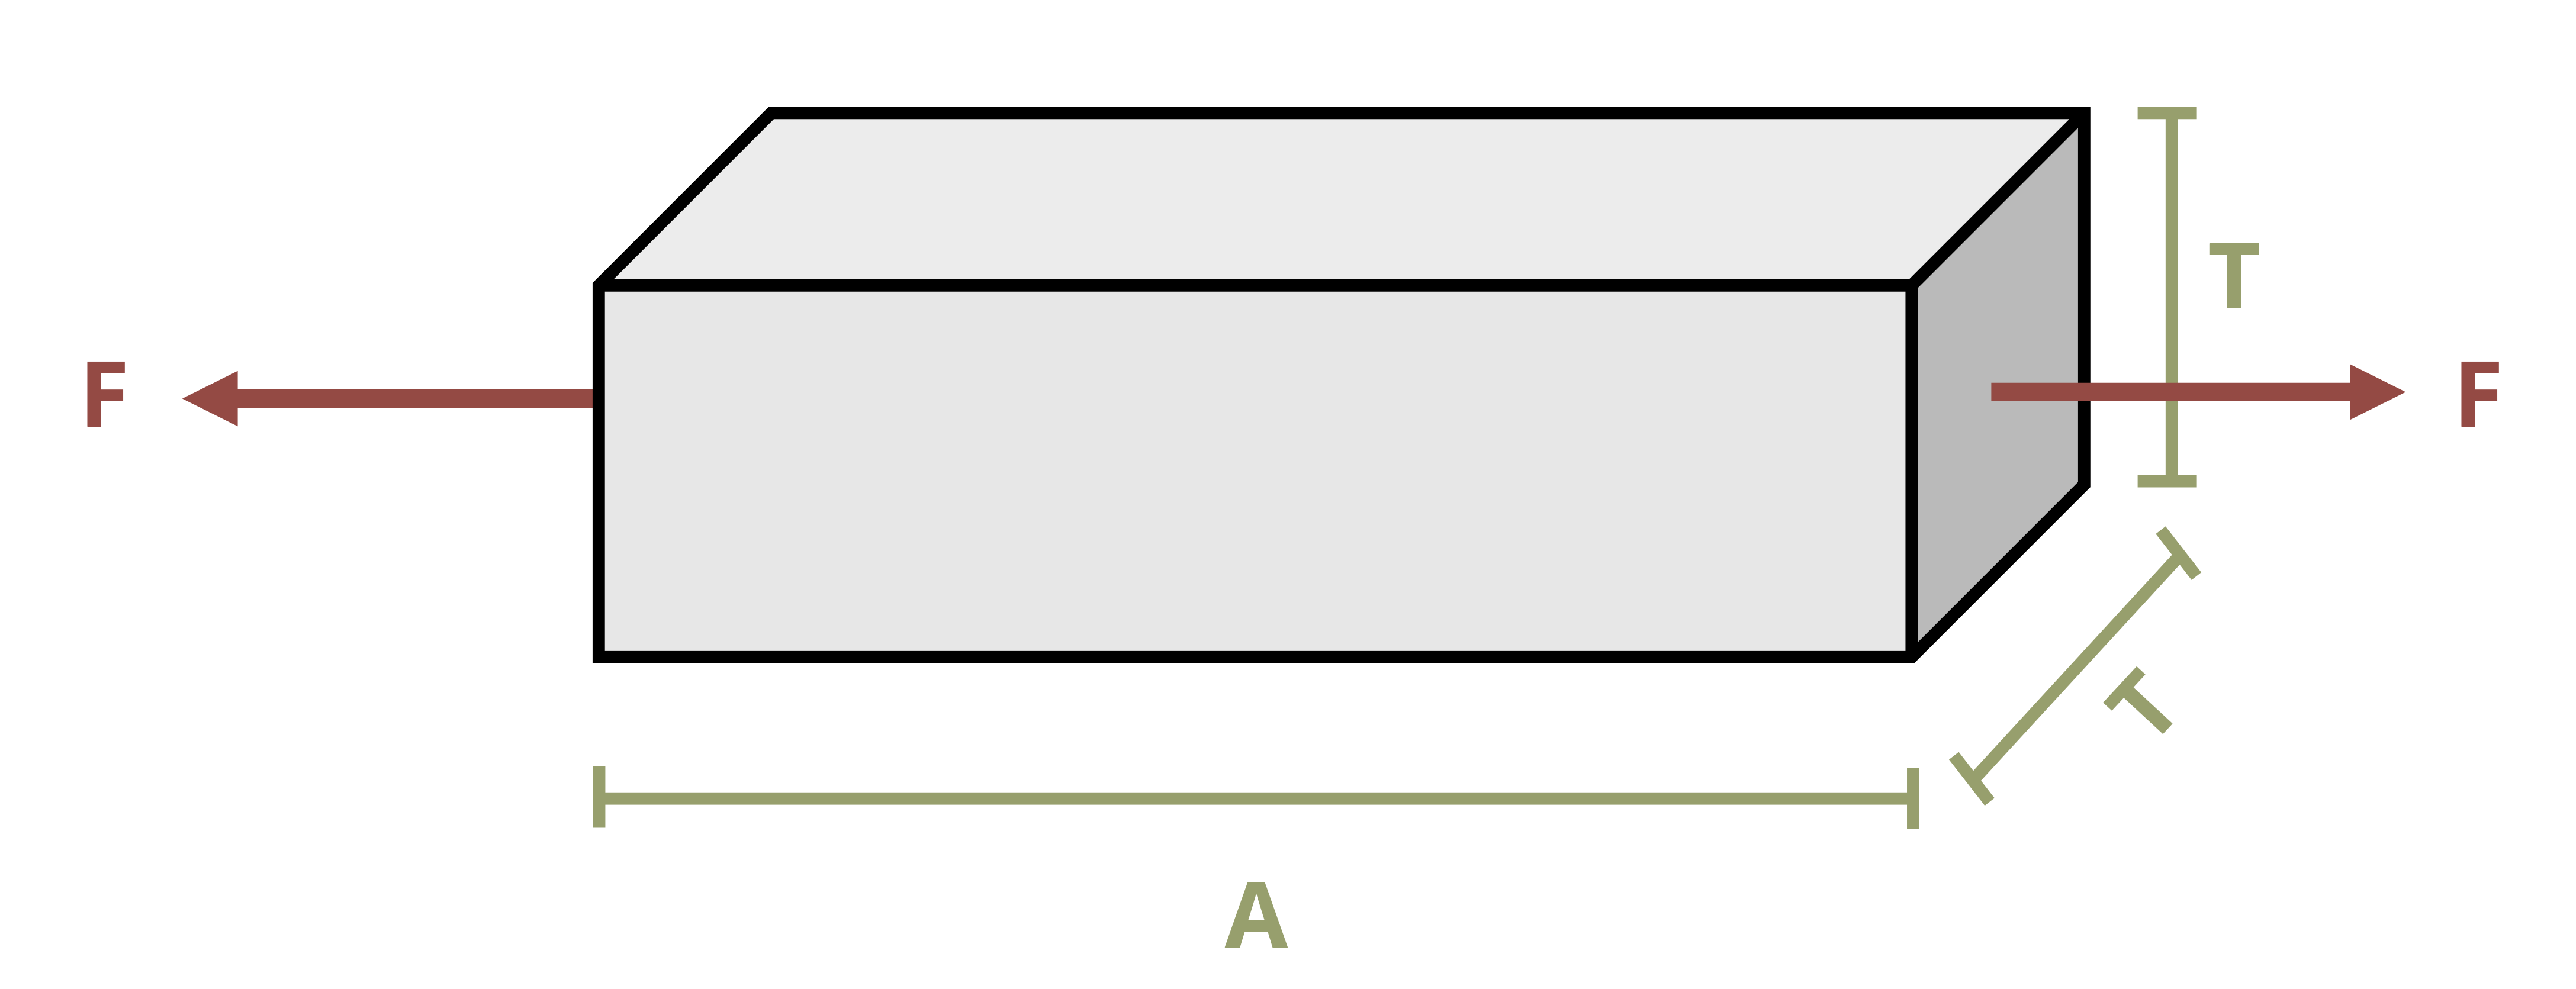
\includegraphics[width=3.76042in,height=\textheight]{images/PNGs/Figure 5.1.png}

}

\caption{Figure 5.1: Axial loads act perpendicular to the cross-section.
They cause normal stress on the cross-section and normal strains in both
the axial (A) and transverse (T) directions.}

\end{figure}%

Axial loads create axial stresses, which we have already seen in Section
2.1 and we'll revisit briefly in Section 5.1. We previously considered
the average normal stress in a cross-section, but the geometry of the
cross-section can cause large localized stresses much higher than the
average. We'll discuss these stress concentrations in Section 5.2.

This text is concerned with both stress and deformation, so in Section
5.3 we'll explore the deformation caused by axial loads. We'll extend
this to a special case of axial deformation involving parallel bars in
Section 5.4, before using our knowledge of axial deformation to help us
solve statically indeterminate problems in Section 5.5. These are
problems where the equilibrium equations are not sufficient to determine
the reaction and internal forces.

Finally we'll investigate the effects of temperature in Section 5.6. As
the temperature of an object changes it will expand or contract. Thus
there can be deformation even in the absence of any applied forces.

\section{Axial Stress}\label{axial-stress}

Click to expand

Axial loads create axial stresses, also known as normal stresses. As
discussed in Section 2.1, the average normal stress is calculated from

\[
\sigma=\frac{N}{A}\]

\emph{where}

\emph{𝜎 = Average normal stress {[}Pa, psi{]}}

\emph{N = Internal normal force {[}N, lb{]}}

\emph{A = Cross-sectional area {[}m\textsuperscript{2},
in.\textsuperscript{2}{]}}

\section{Stress Concentrations}\label{stress-concentrations}

Click to expand

The normal stress discussed in the previous section is averaged over the
cross-section and assumes that stresses (and therefore strains) at the
cross-section are uniform. In reality stresses and strains can vary
across a cross-section, especially if the cross-section is close to an
applied load, a support, or a change in geometry. At these points
localized stress concentrations occur, leading to large, localized
stresses and strains. The intensity of these concentrations depends on
the type of loading, support, or geometry (Figure 5.2).

\begin{figure}[H]

{\centering 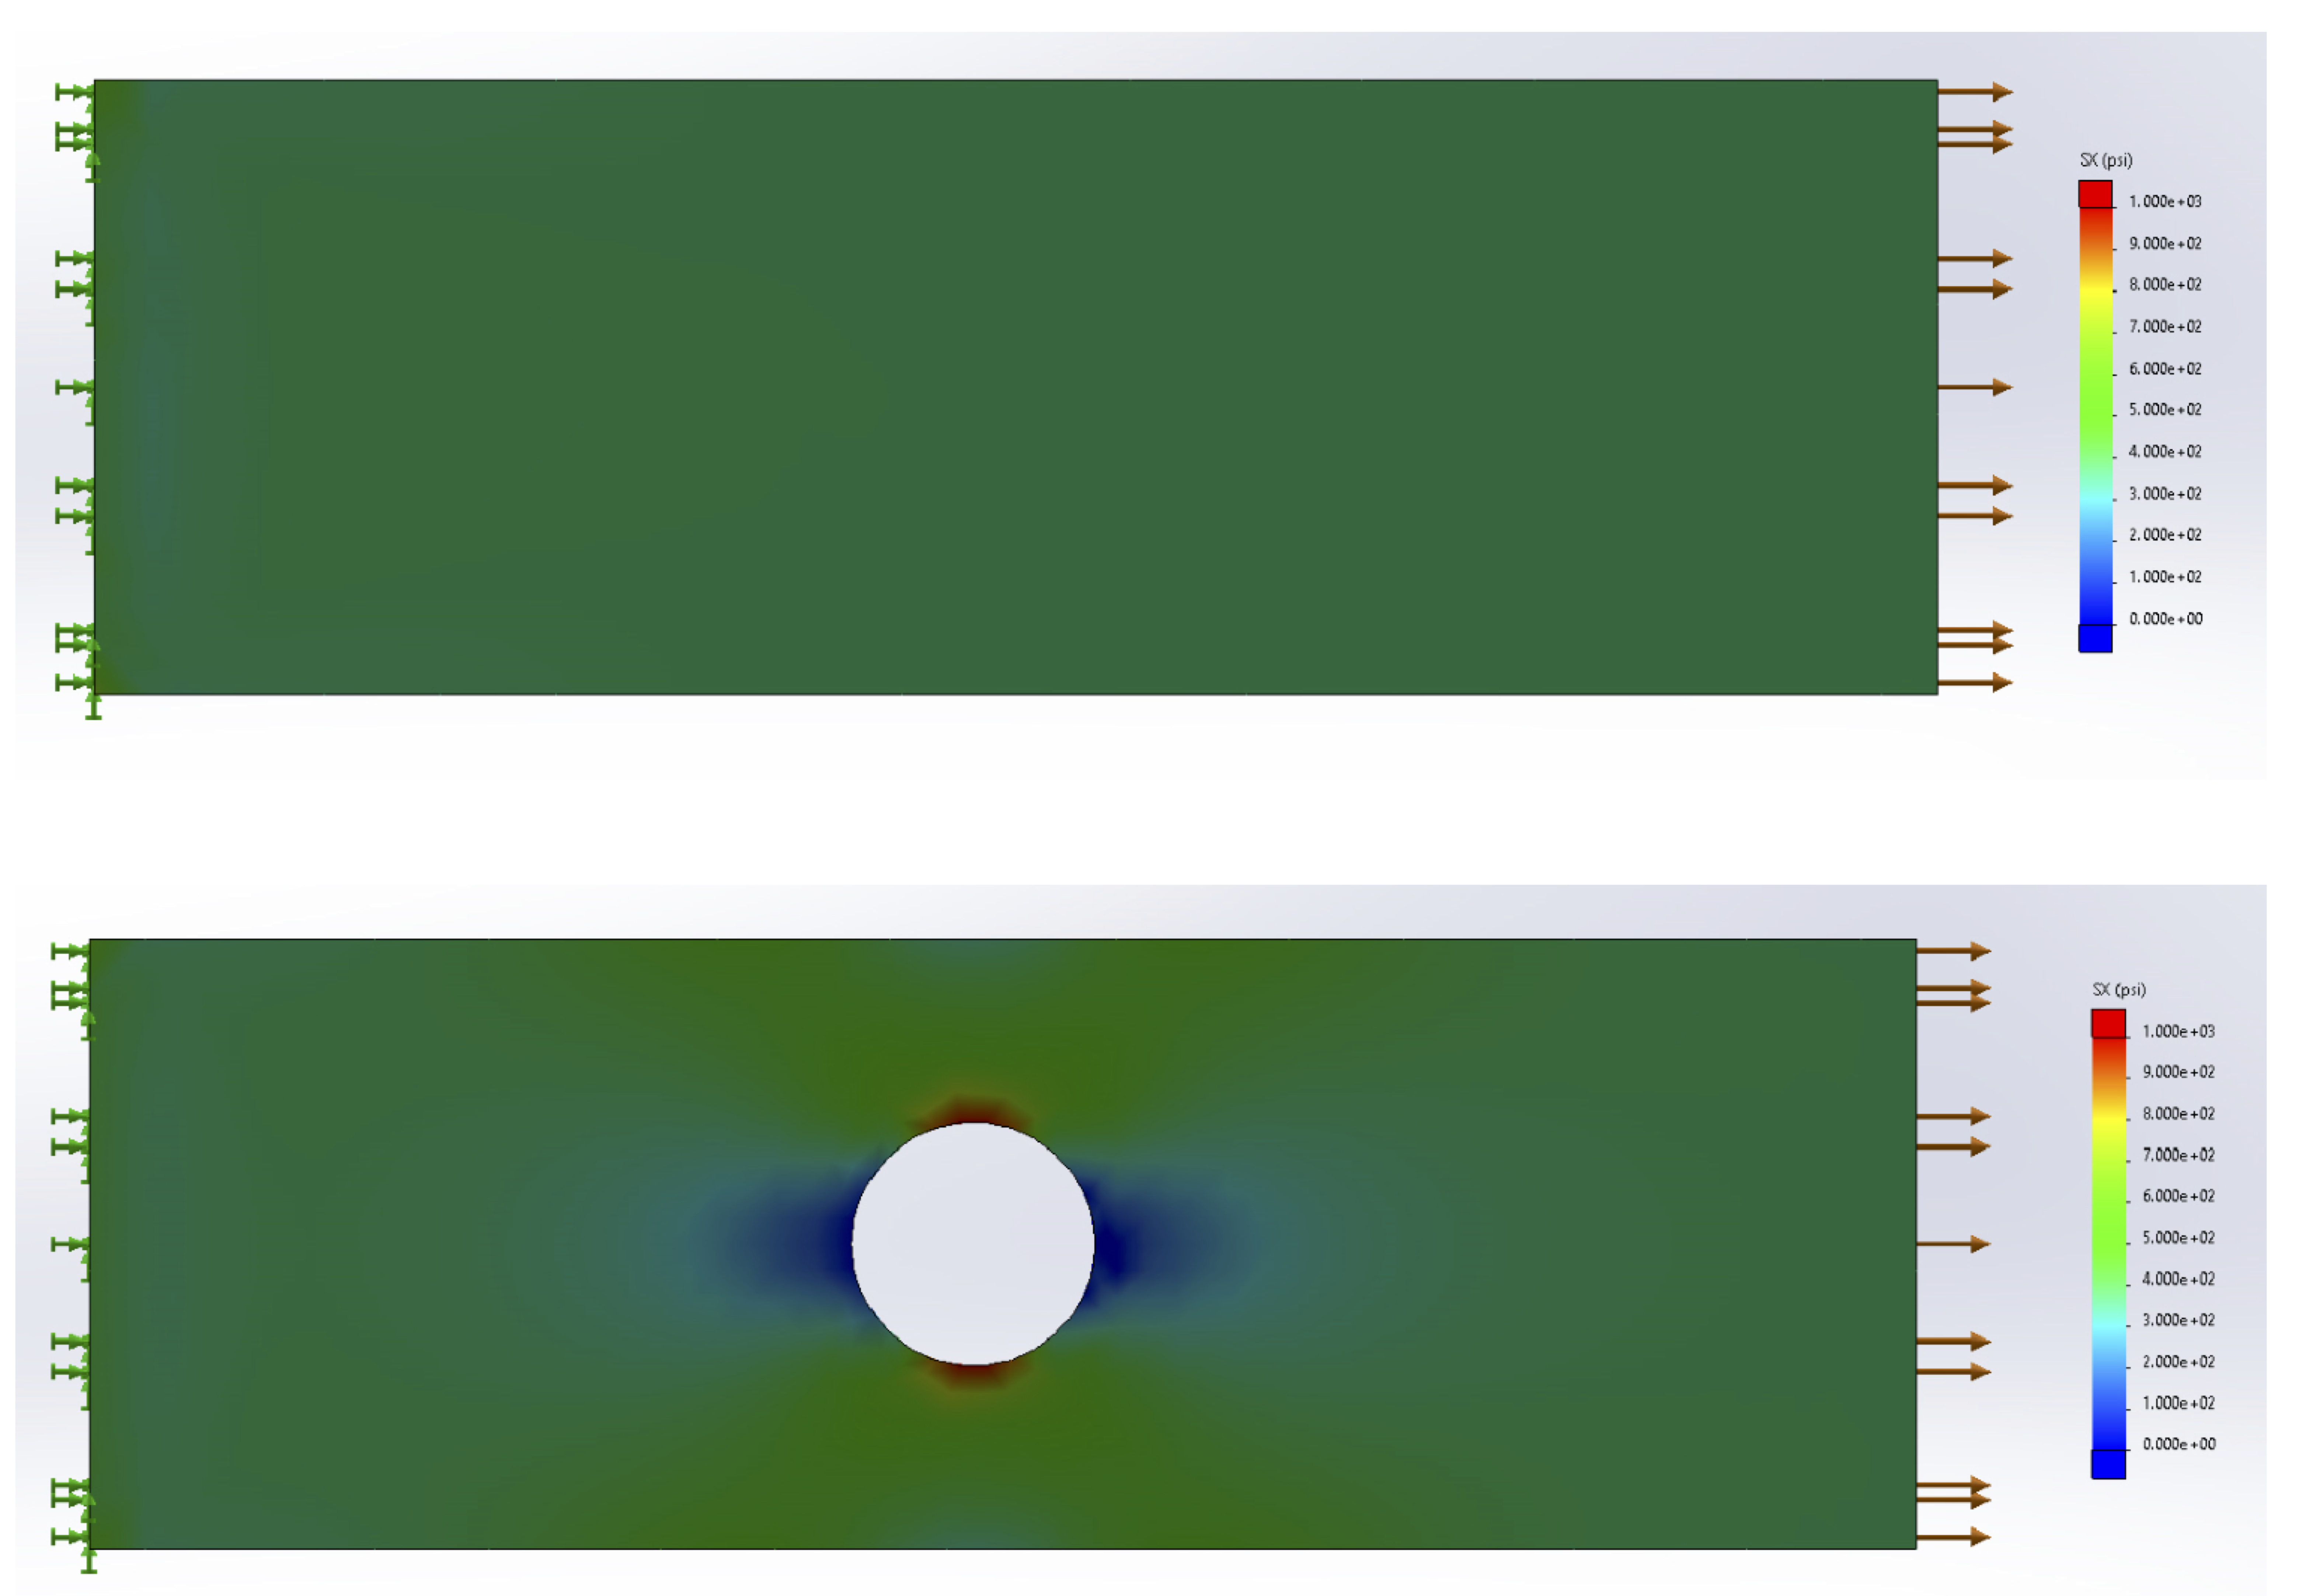
\includegraphics[width=5.89583in,height=\textheight]{images/PNGs/Figure 5.2.png}

}

\caption{Figure 5.2: Each bar has a fixed support on the left, a
cross-section of 30 in.², and is subjected to a force of 10,000 lb. The
top bar is uniform and experiences a uniform average normal stress of
\$\textbackslash sigma=\textbackslash frac\{10000\}\{30\}=333\$ psi at
all points, except those close to the support and load. The bottom bar
experiences the same stress at most points, but significantly higher
stress concentrations close to the hole.}

\end{figure}%

However, these effects disappear a certain distance away from the force,
support, or local geometry. It is therefore acceptable to assume uniform
stress and strain (as we have been so far) provided that we also assume
our cross-section is a sufficient distance away from these points. This
is known as Saint-Venant's principle, which can be formally stated as
``The stresses and strains created at a point in a body by two
statically equivalent loads are equivalent at points sufficiently far
removed from the applied load'' (Figure 5.3).

\begin{figure}[H]

{\centering 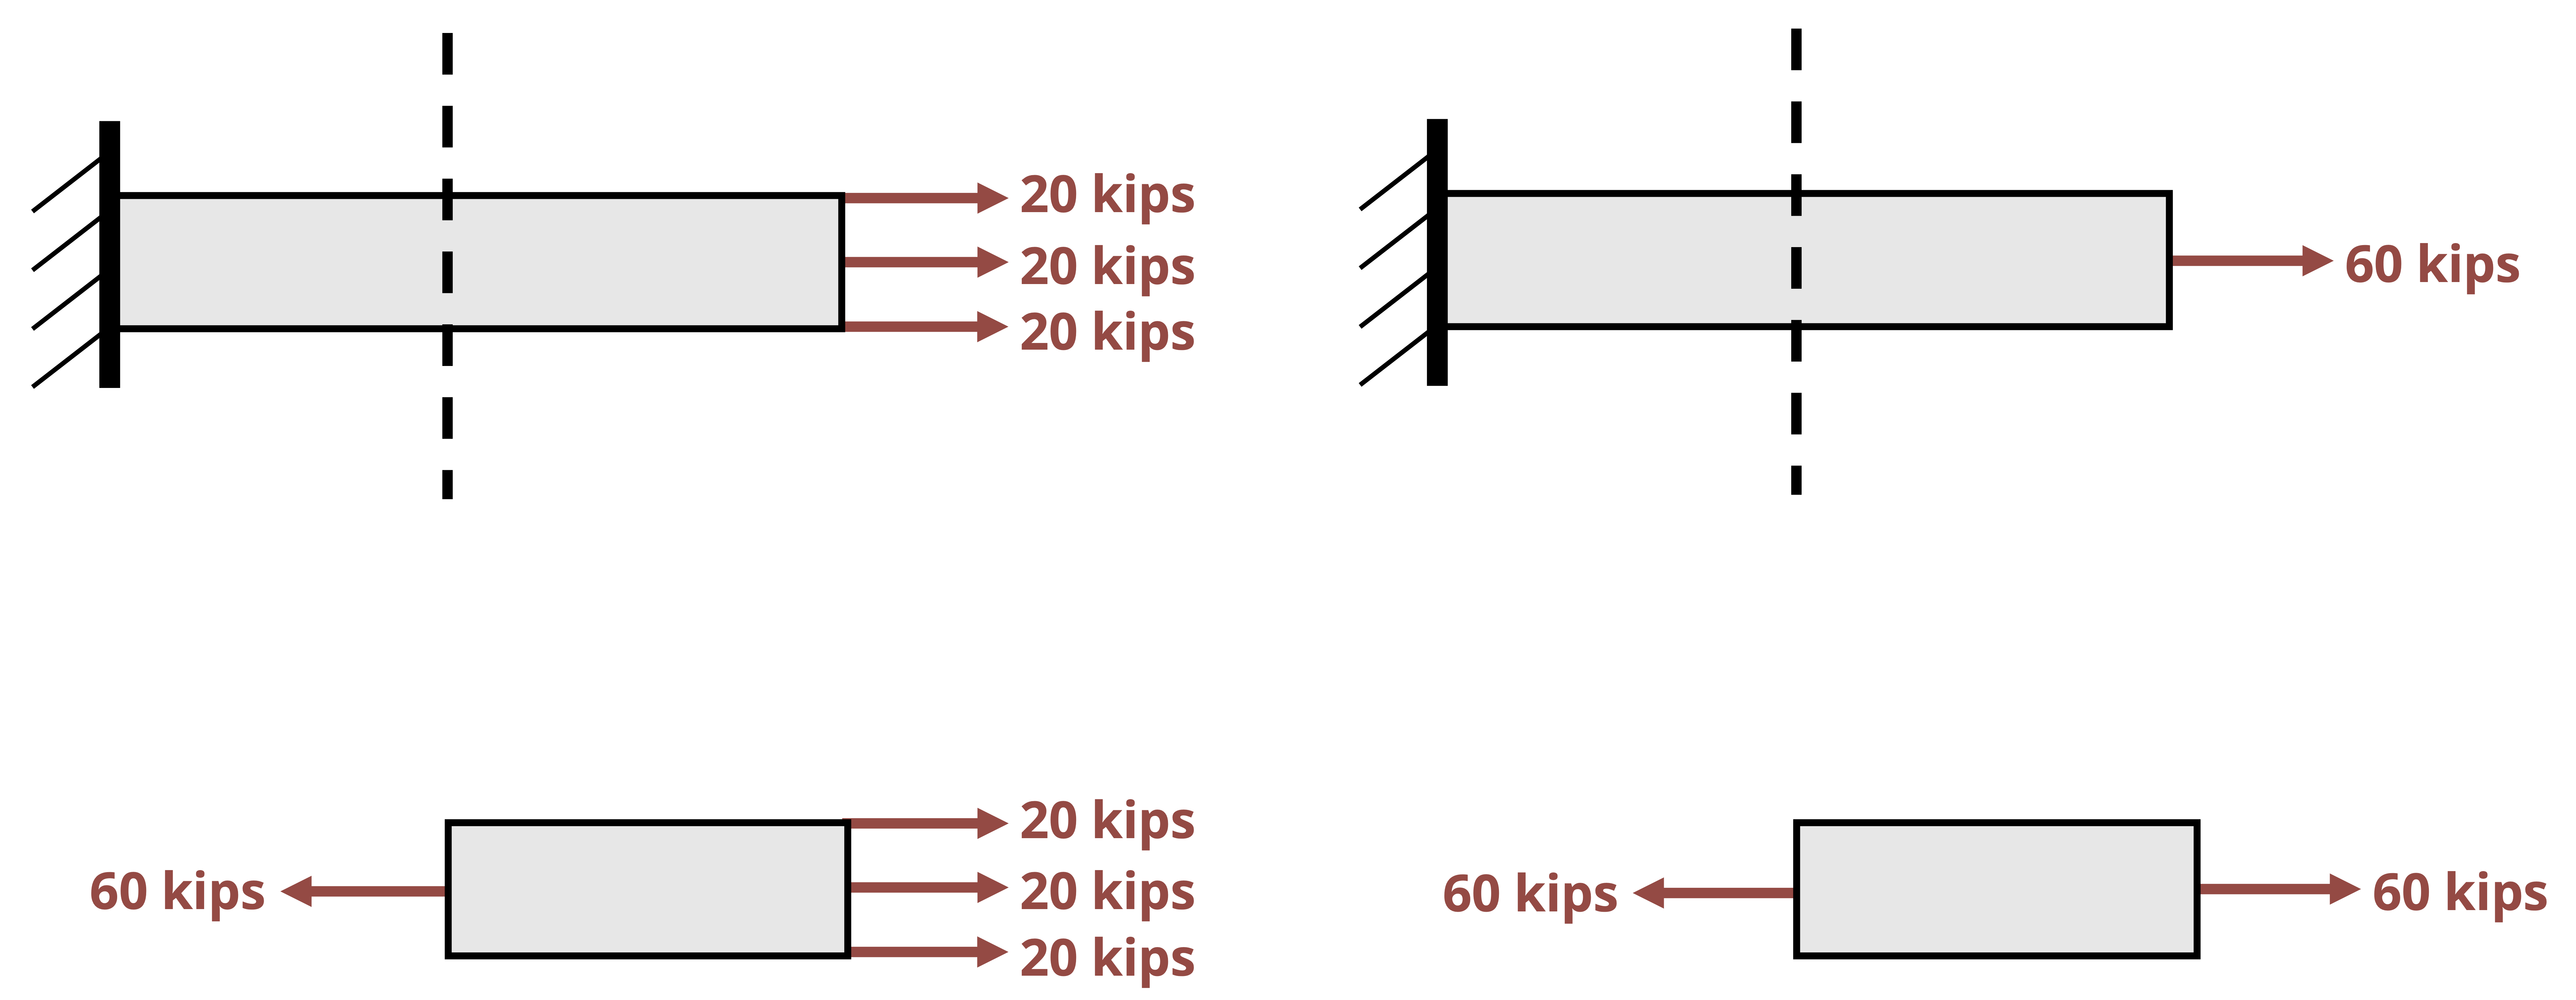
\includegraphics[width=5.88542in,height=\textheight]{images/PNGs/Figure 5.3.png}

}

\caption{Figure 5.3: Two statically equivalent loads applied to a bar.
Close to the point of application there will be localized stresses and
deformations, but at a cross-section sufficiently far away from the
applied loads the internal effects are equivalent.}

\end{figure}%

More advanced courses will use the theory of elasticity to study the
areas of variable stress and strain, but for now we'll continue to apply
Saint-Venant's principle and assume that our cross-sections are
sufficiently far away from the applied loads that we don't need to
consider these stress concentrations. We will however address the
question of stress concentrations around changes in geometry here. We'll
study two specific examples; holes and fillets. Figure 5.2 shows an
example of the stress concentrations around a hole. Figure 5.4 shows an
example of the stress concentrations around a fillet. A fillet is a
rounded corner used to help transition between two geometries.

\begin{figure}[H]

{\centering 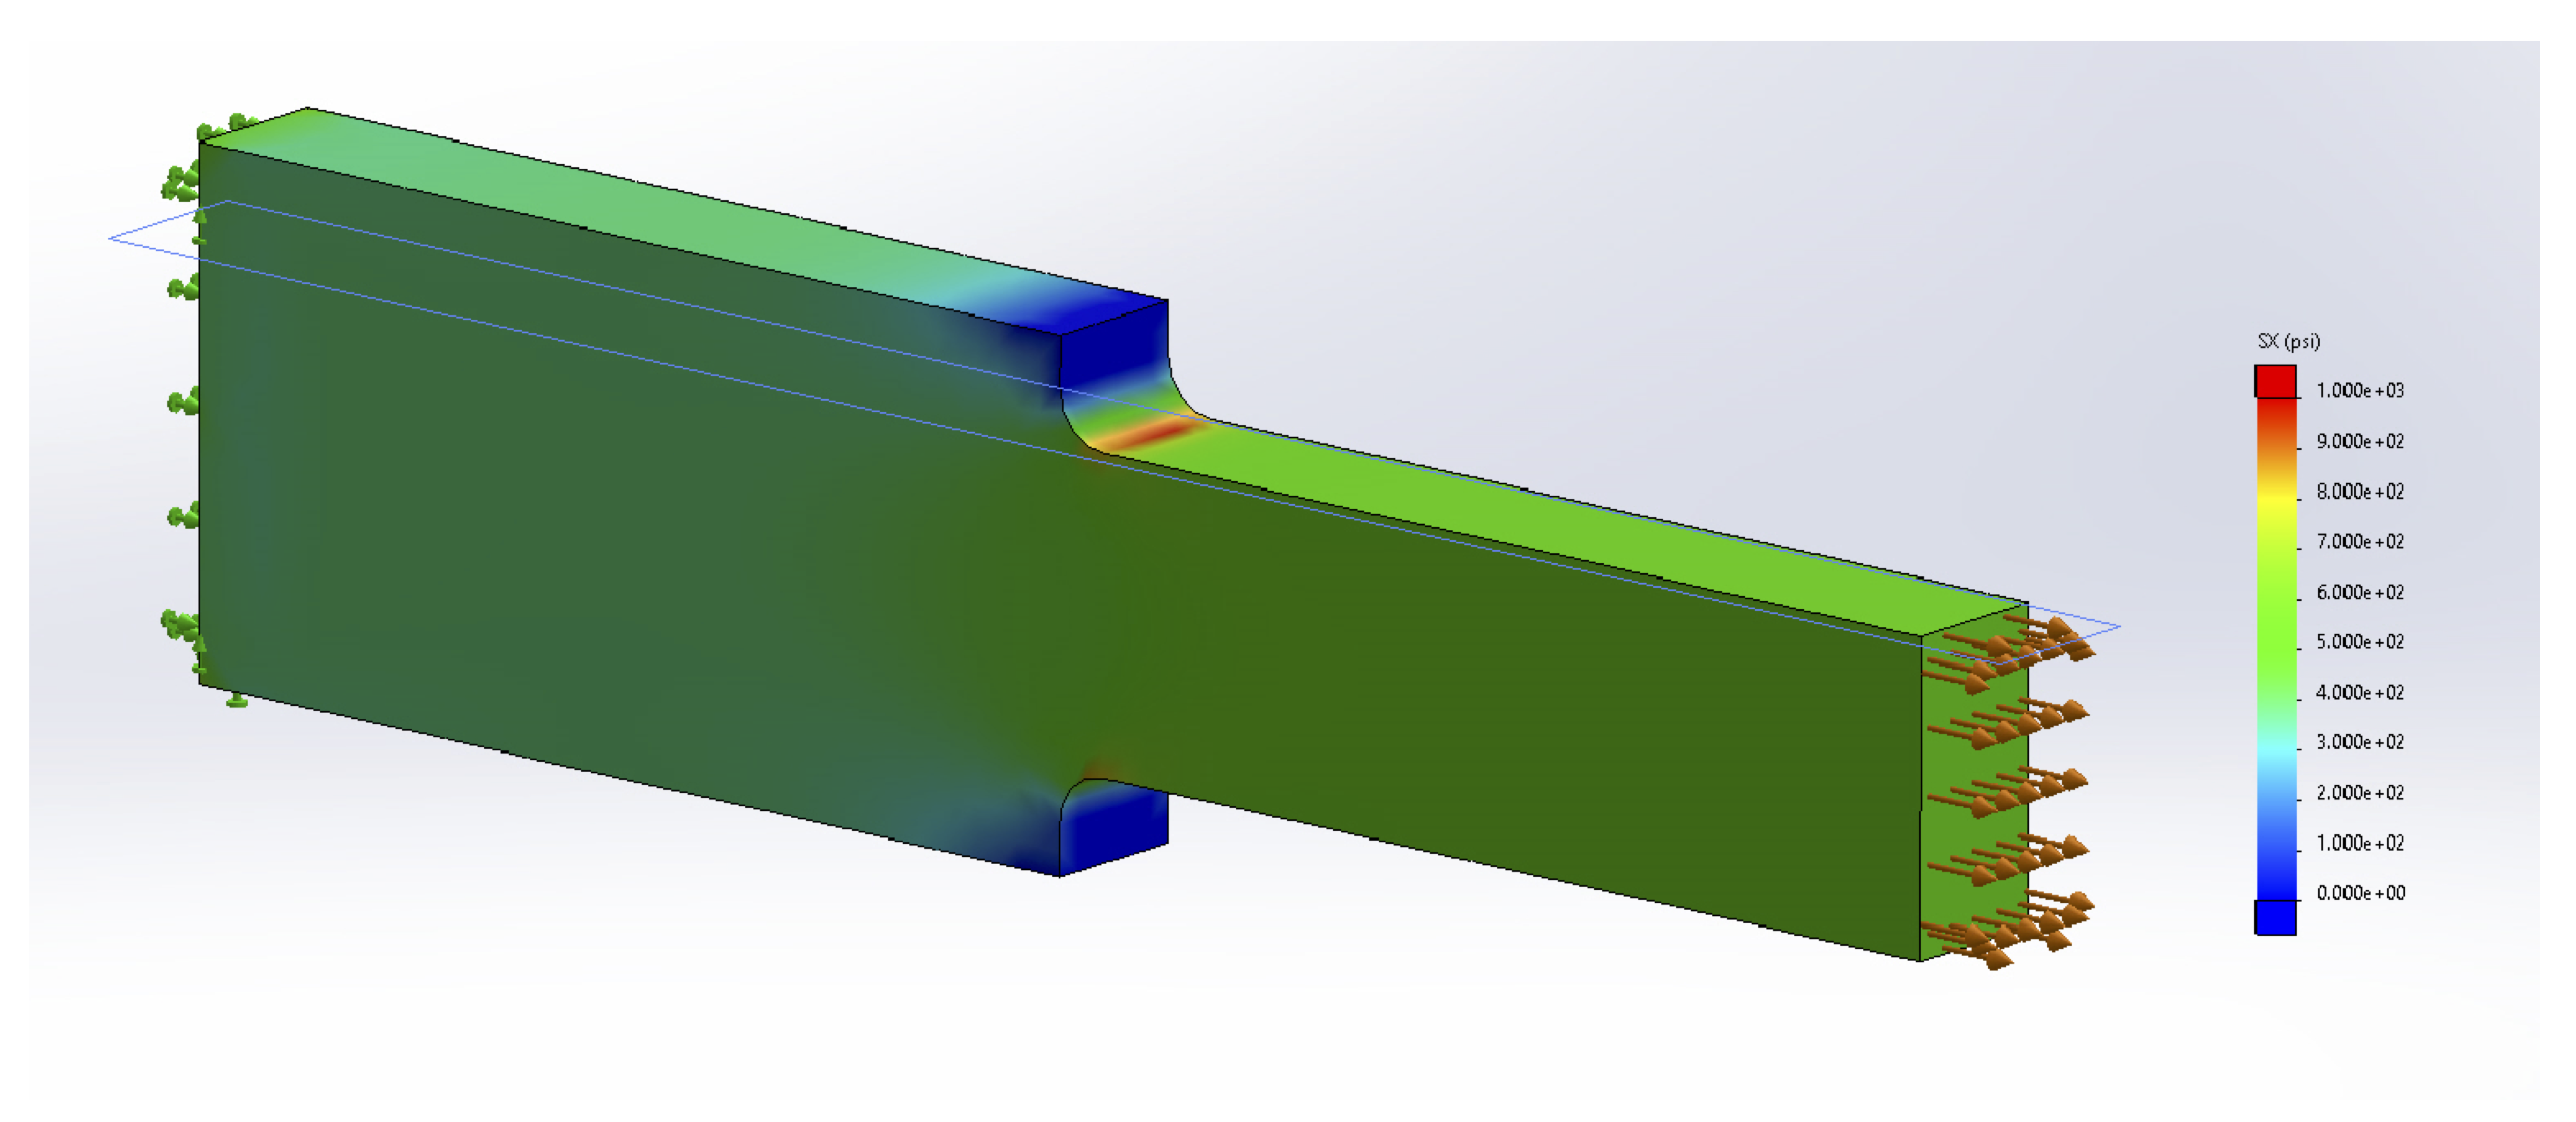
\includegraphics{images/PNGs/Figure 5.4.png}

}

\caption{Figure 5.4: The fillet helps prevent a sharp corner but still
causes stress concentrations. The bar has a thickness of 3 in. The
height of the smaller section is 6 in. and the larger section is 10 in.
The applied load is 10,000 kips, so the average normal stress in the
smaller section is 556 psi and in the larger section is 333 psi. The
maximum stress at the fillet however is 973 psi.}

\end{figure}%

Fully modeling these stress concentrations is very complicated, but for
our purposes it is sufficient to find only the maximum stress that
occurs around these stress concentrations. These can be significantly
larger than the average stress we have been calculating, and can cause
localized failure even if the average stress is below the yield stress
for the material. The maximum stress can be found simply by multiplying
the average stress by a stress concentration factor, K.

\[
\sigma_{\text {max }}=K \sigma_{\text {avg }}\]

\emph{where}

\emph{𝜎\textsubscript{max} = Maximum normal stress {[}Pa, psi{]}}

\emph{K = Stress concentrtion factor {[}unitless{]}}

\emph{𝜎\textsubscript{avg} = Average normal stress {[}Pa, psi{]}}

This stress concentration factor depends on the geometry at hand and can
be found from curves in design handbooks (Figure 5.5). See Examples 5.1
and 5.2 to see how these curves can be used.

\begin{figure}[H]

{\centering 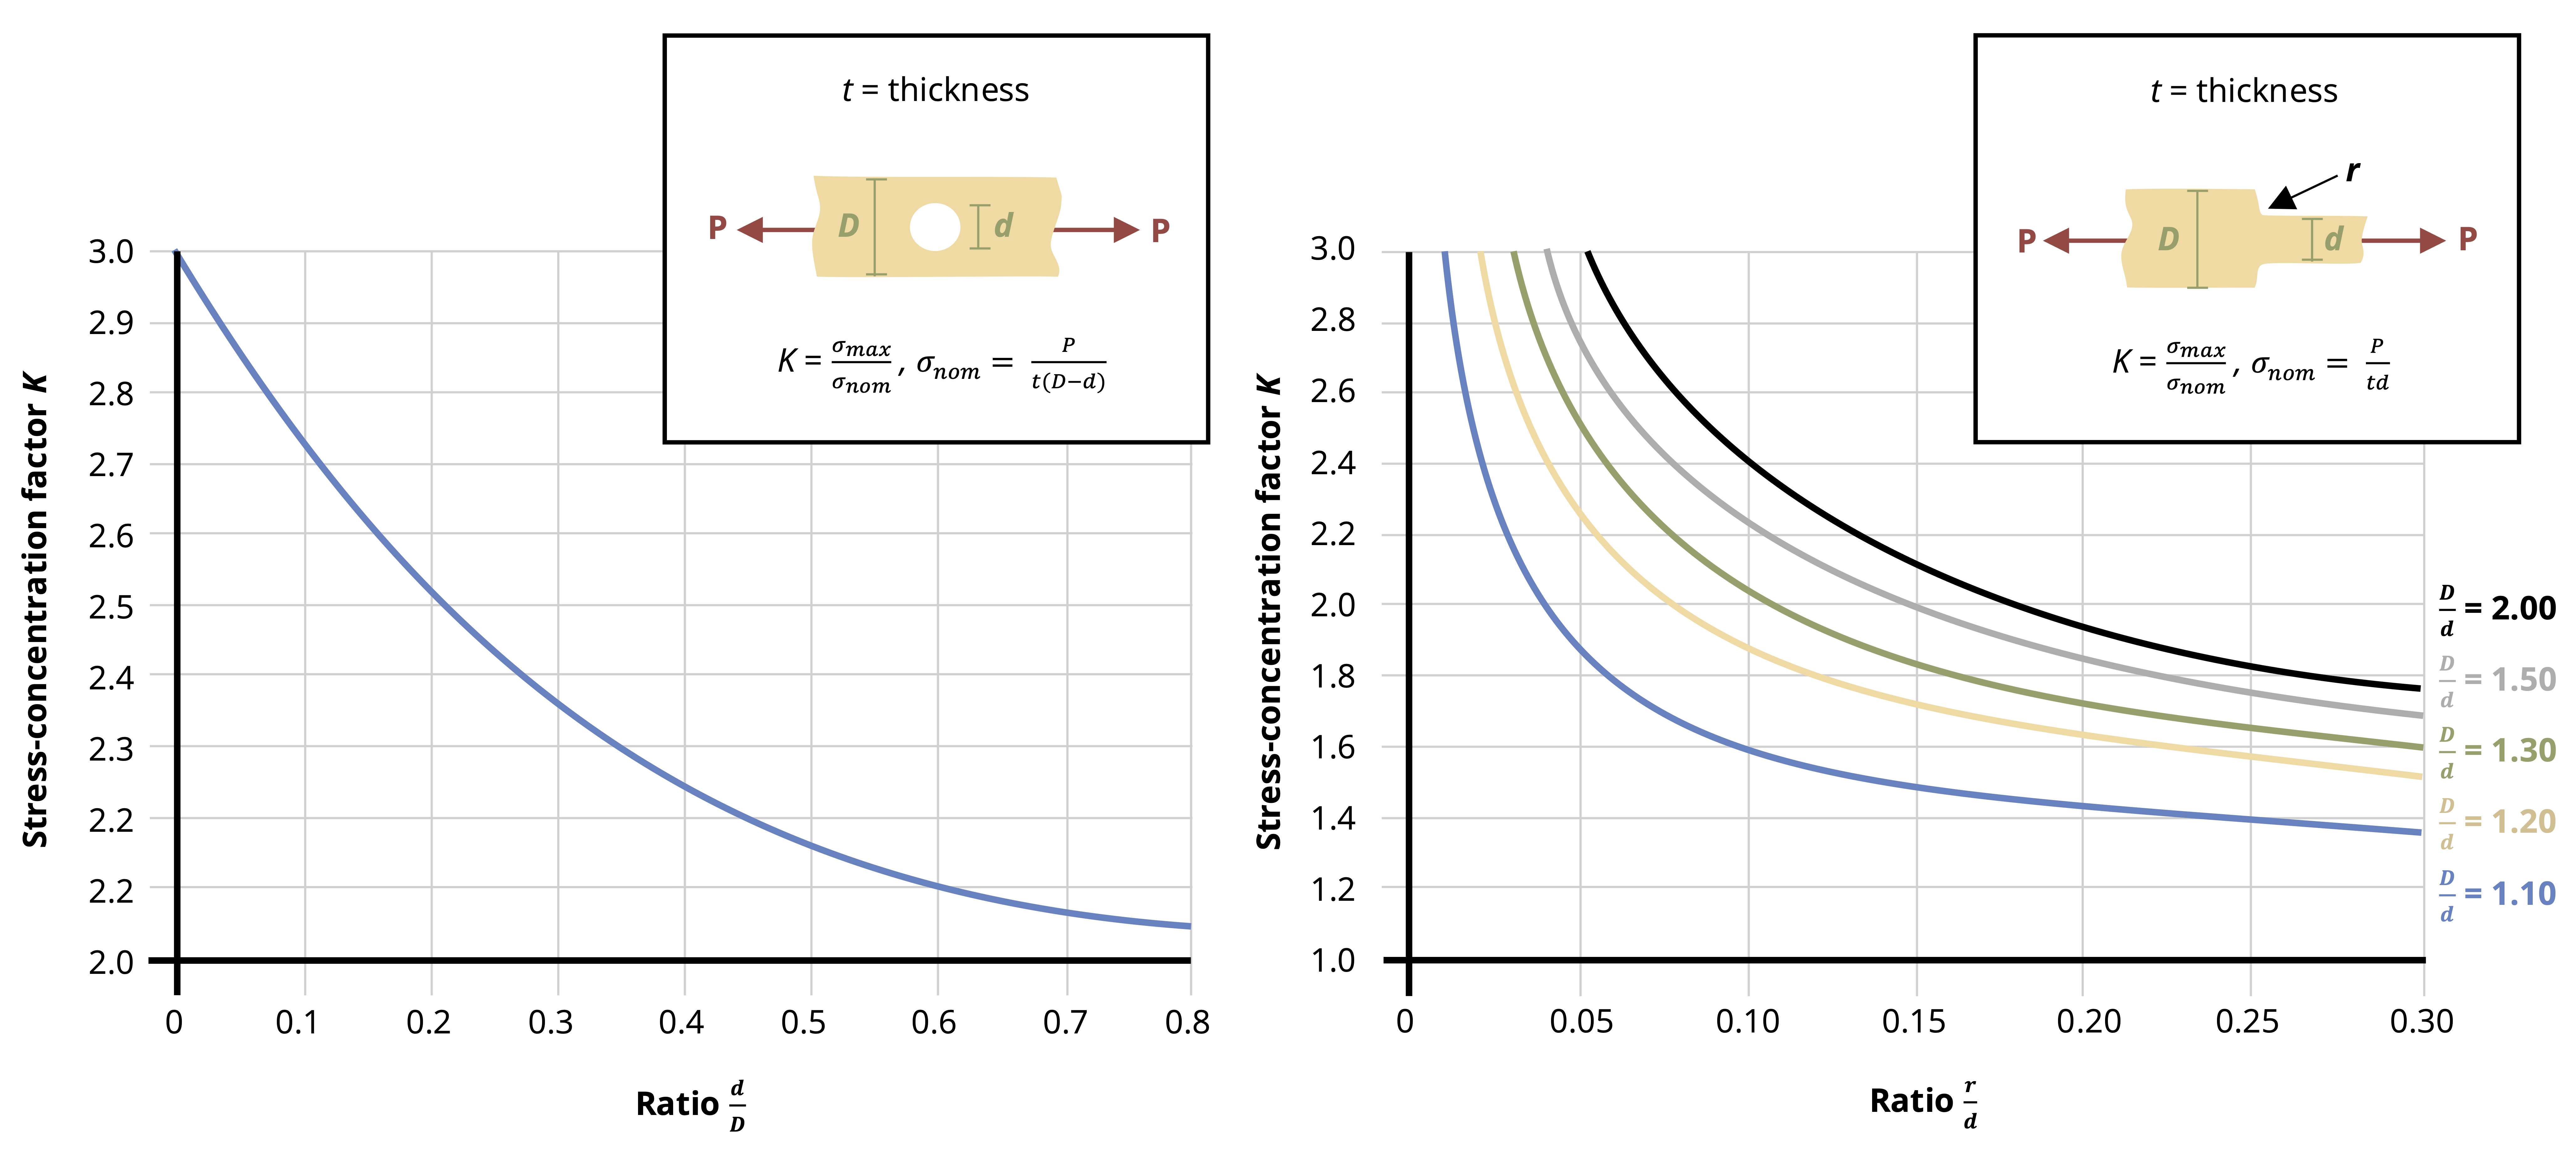
\includegraphics{images/PNGs/Figure 5.5.png}

}

\caption{Figure 5.5: Graphs showing how the stress concentration factor,
K changes based on the geometry of the object.}

\end{figure}%

\begin{tcolorbox}[enhanced jigsaw, colback=white, colframe=quarto-callout-note-color-frame, leftrule=.75mm, opacitybacktitle=0.6, colbacktitle=quarto-callout-note-color!10!white, arc=.35mm, bottomrule=.15mm, breakable, title={Example 5.1: Stress concentration for hole}, left=2mm, titlerule=0mm, toptitle=1mm, toprule=.15mm, opacityback=0, rightrule=.15mm, coltitle=black, bottomtitle=1mm]

A hole is drilled through a steel plate to allow two components to be
bolted together. The plate has the dimensions shown and is 15 mm thick.
If the plate is subjected to an axial load of P = 50 kN, determine the
maximum stress in the plate if the hole diameter d = 20 mm.

\begin{center}
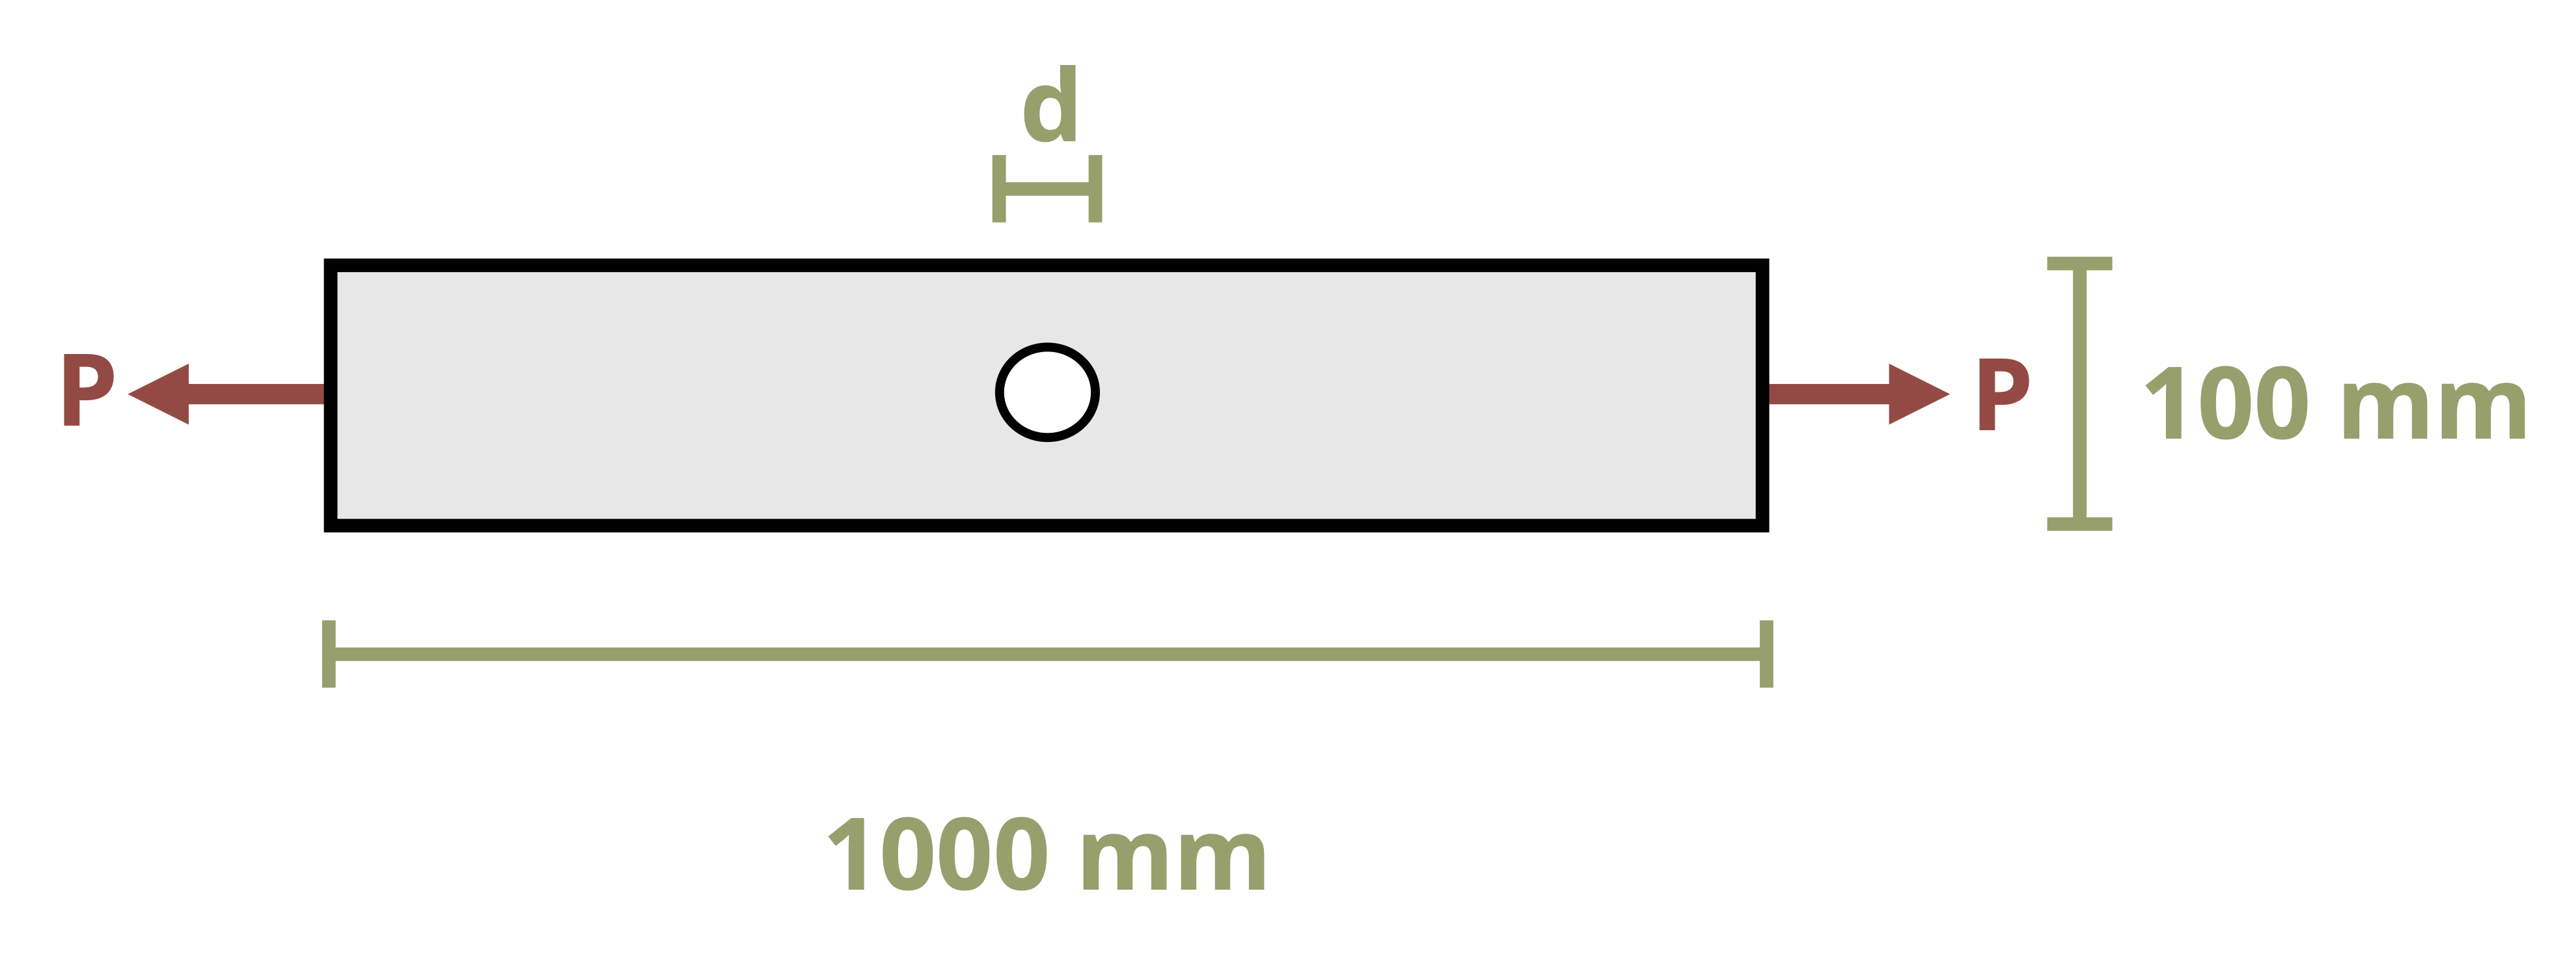
\includegraphics[width=3.625in,height=\textheight]{images/PNGs/Example 5.1 part 1.png}
\end{center}

\begin{tcolorbox}[enhanced jigsaw, colback=white, colframe=quarto-callout-note-color-frame, leftrule=.75mm, opacitybacktitle=0.6, colbacktitle=quarto-callout-note-color!10!white, arc=.35mm, bottomrule=.15mm, breakable, title={Solution}, left=2mm, titlerule=0mm, toptitle=1mm, toprule=.15mm, opacityback=0, rightrule=.15mm, coltitle=black, bottomtitle=1mm]

Start by calculating the average normal stress in the plate at the
location of the hole. The cross-section is a rectangle with a base of 15
mm (0.015 m) and a height of 100 mm (0.1 m), with a 20 mm (0.02 m)
diameter hole cut out.

\begin{center}
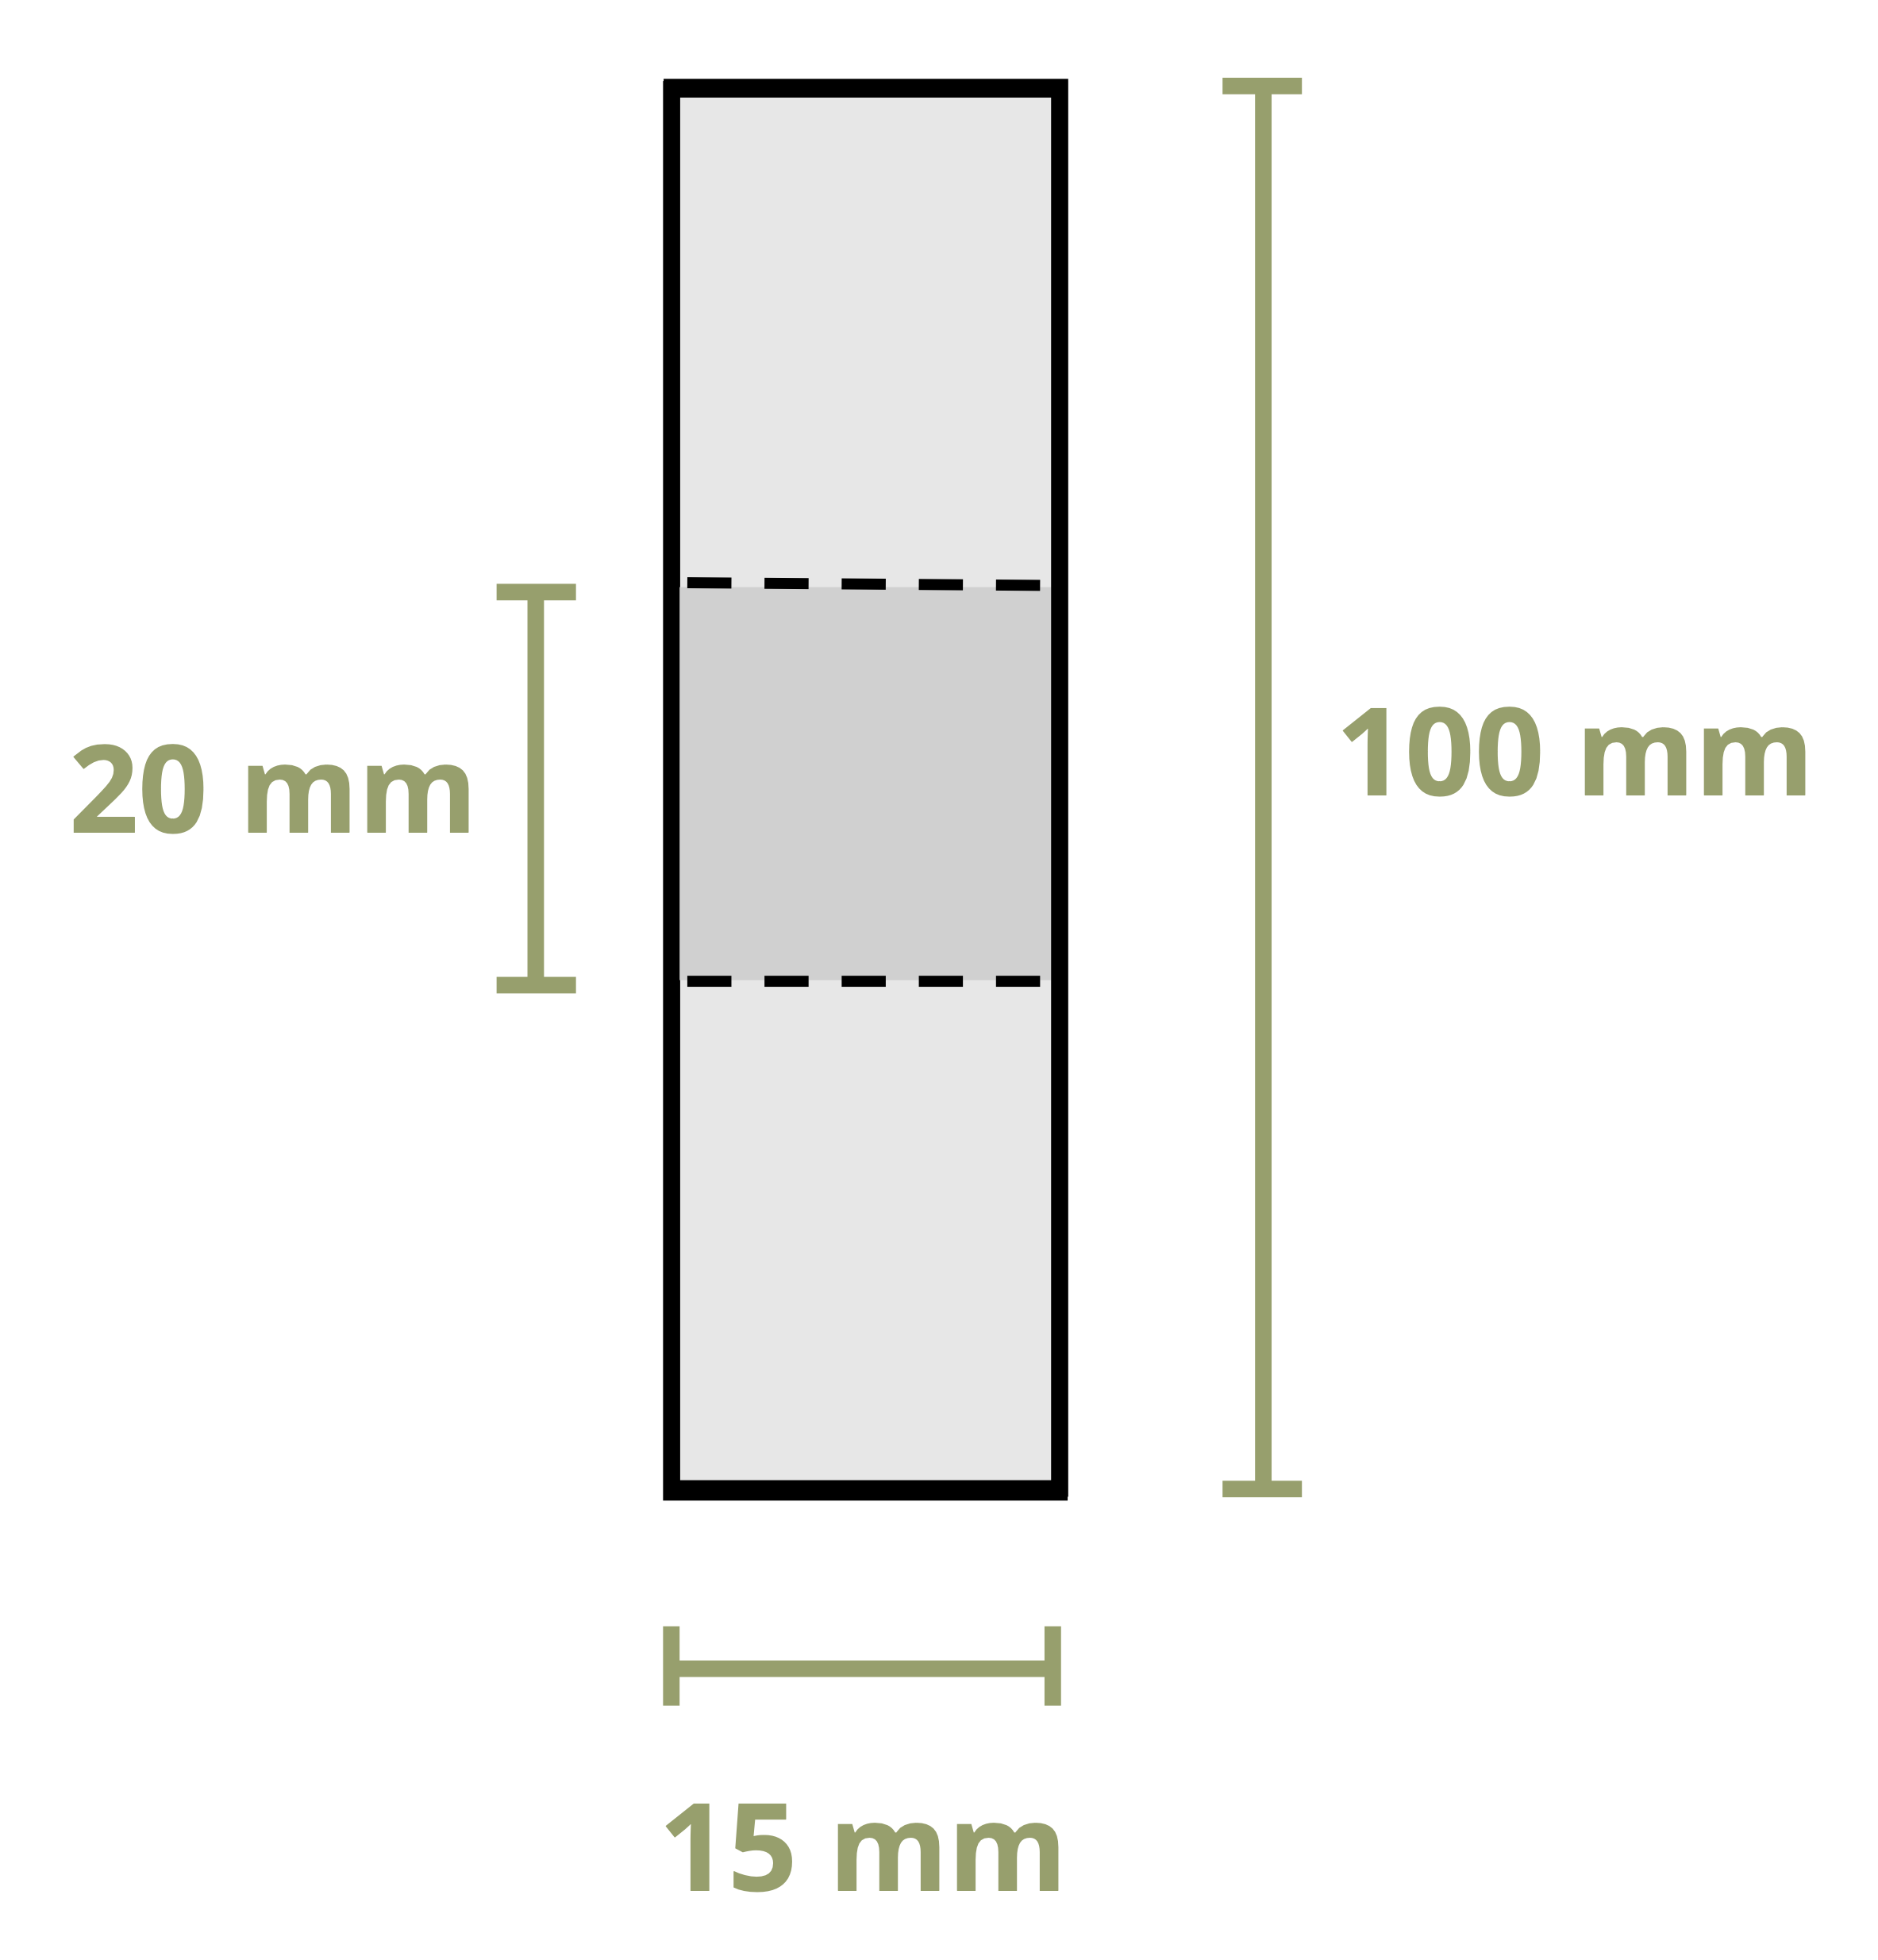
\includegraphics[width=1.92708in,height=\textheight]{images/PNGs/Example 5.1 part 2.png}
\end{center}

\[
\sigma_{a v g}=\frac{N}{A}=\frac{50000}{0.015 *(0.1-0.02)}=41.7 \mathrm{MPa}
\]

Determine the ratio \(\frac{d}{D}\) where d = hole diameter and D =
Height of the cross-section. Use the appropriate stress concentration
curve to read off the stress concentration factor K for this geometry.

\begin{center}
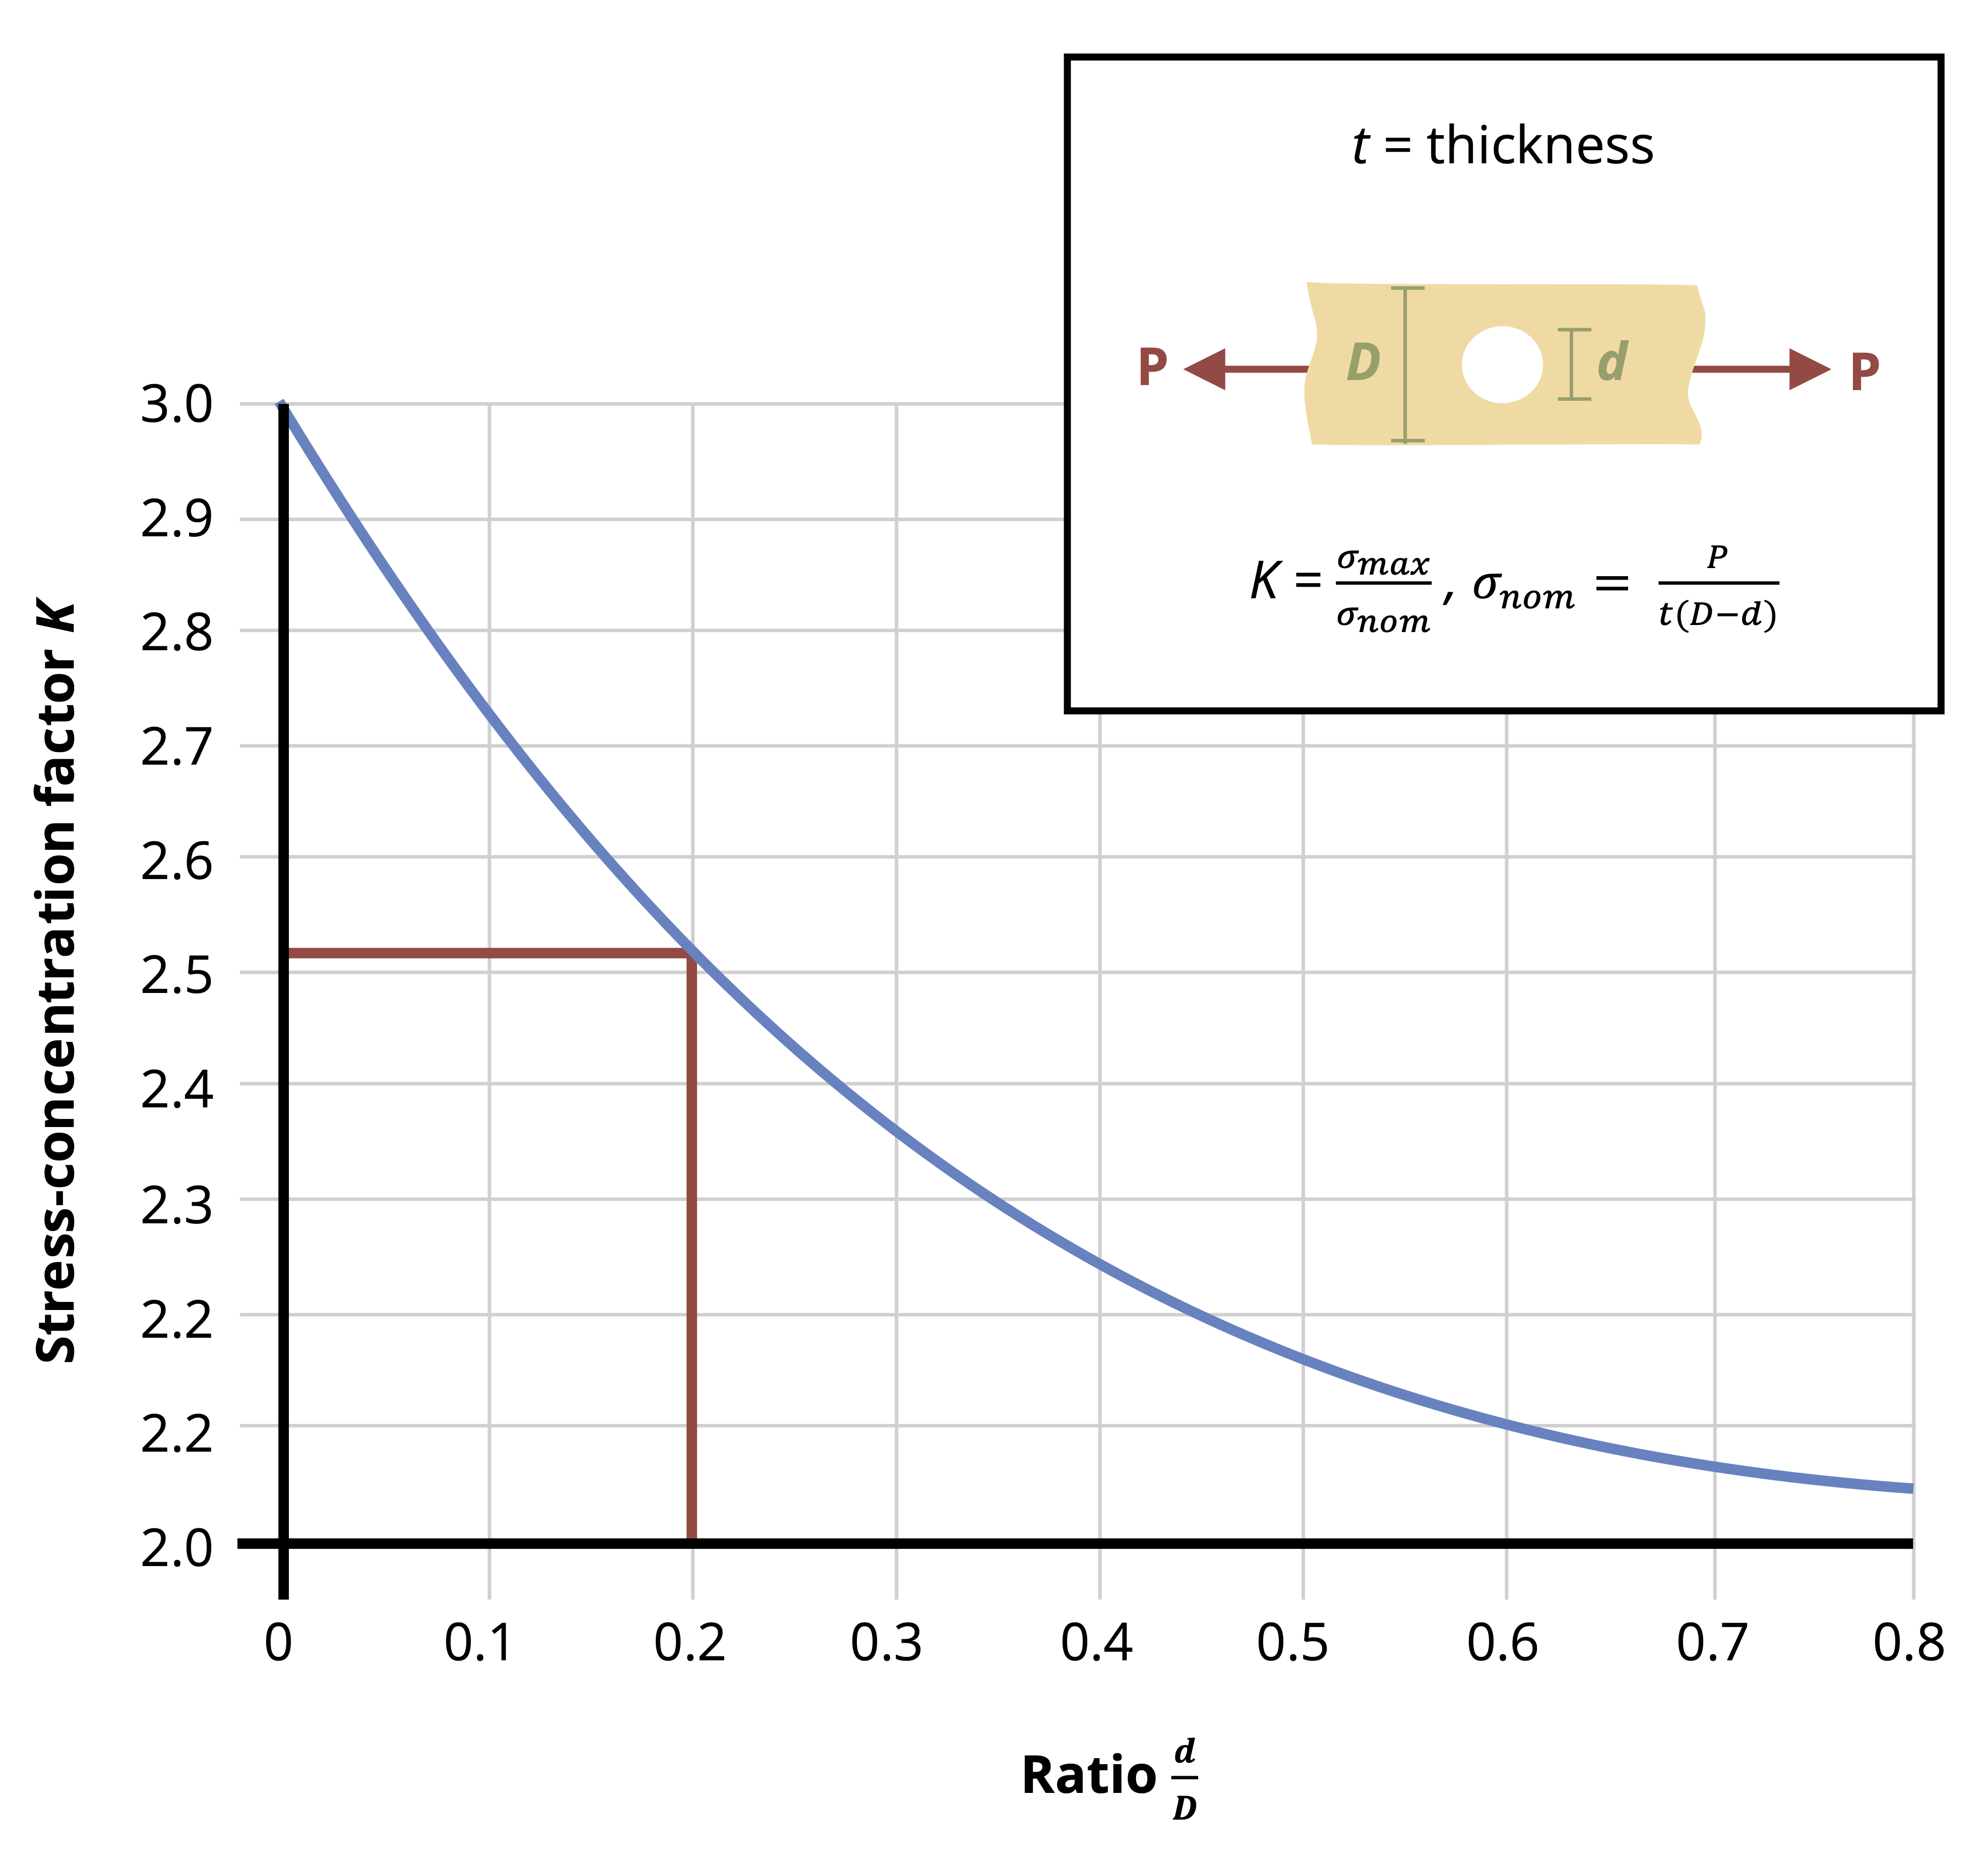
\includegraphics[width=4.02083in,height=\textheight]{images/PNGs/Example 5.1 part 3.png}
\end{center}

\[
\begin{aligned}
&\frac{d}{D}=\frac{20}{100}=0.2\\
&K=2.525
\end{aligned}
\]

Calculate the maximum stress.

\[
\sigma_{\max }=K \sigma_{a v g}=2.525 * 41.7=105 M P a
\]

\end{tcolorbox}

\end{tcolorbox}

\begin{tcolorbox}[enhanced jigsaw, colback=white, colframe=quarto-callout-note-color-frame, leftrule=.75mm, opacitybacktitle=0.6, colbacktitle=quarto-callout-note-color!10!white, arc=.35mm, bottomrule=.15mm, breakable, title={Example 5.2: Stress concentration for fillet}, left=2mm, titlerule=0mm, toptitle=1mm, toprule=.15mm, opacityback=0, rightrule=.15mm, coltitle=black, bottomtitle=1mm]

A 1-inch-thick connecting rod in an engine assembly has the dimensions
shown. If the maximum allowable stress in the rod is 40 ksi, determine
the maximum axial load that may be applied to the rod.

\begin{center}
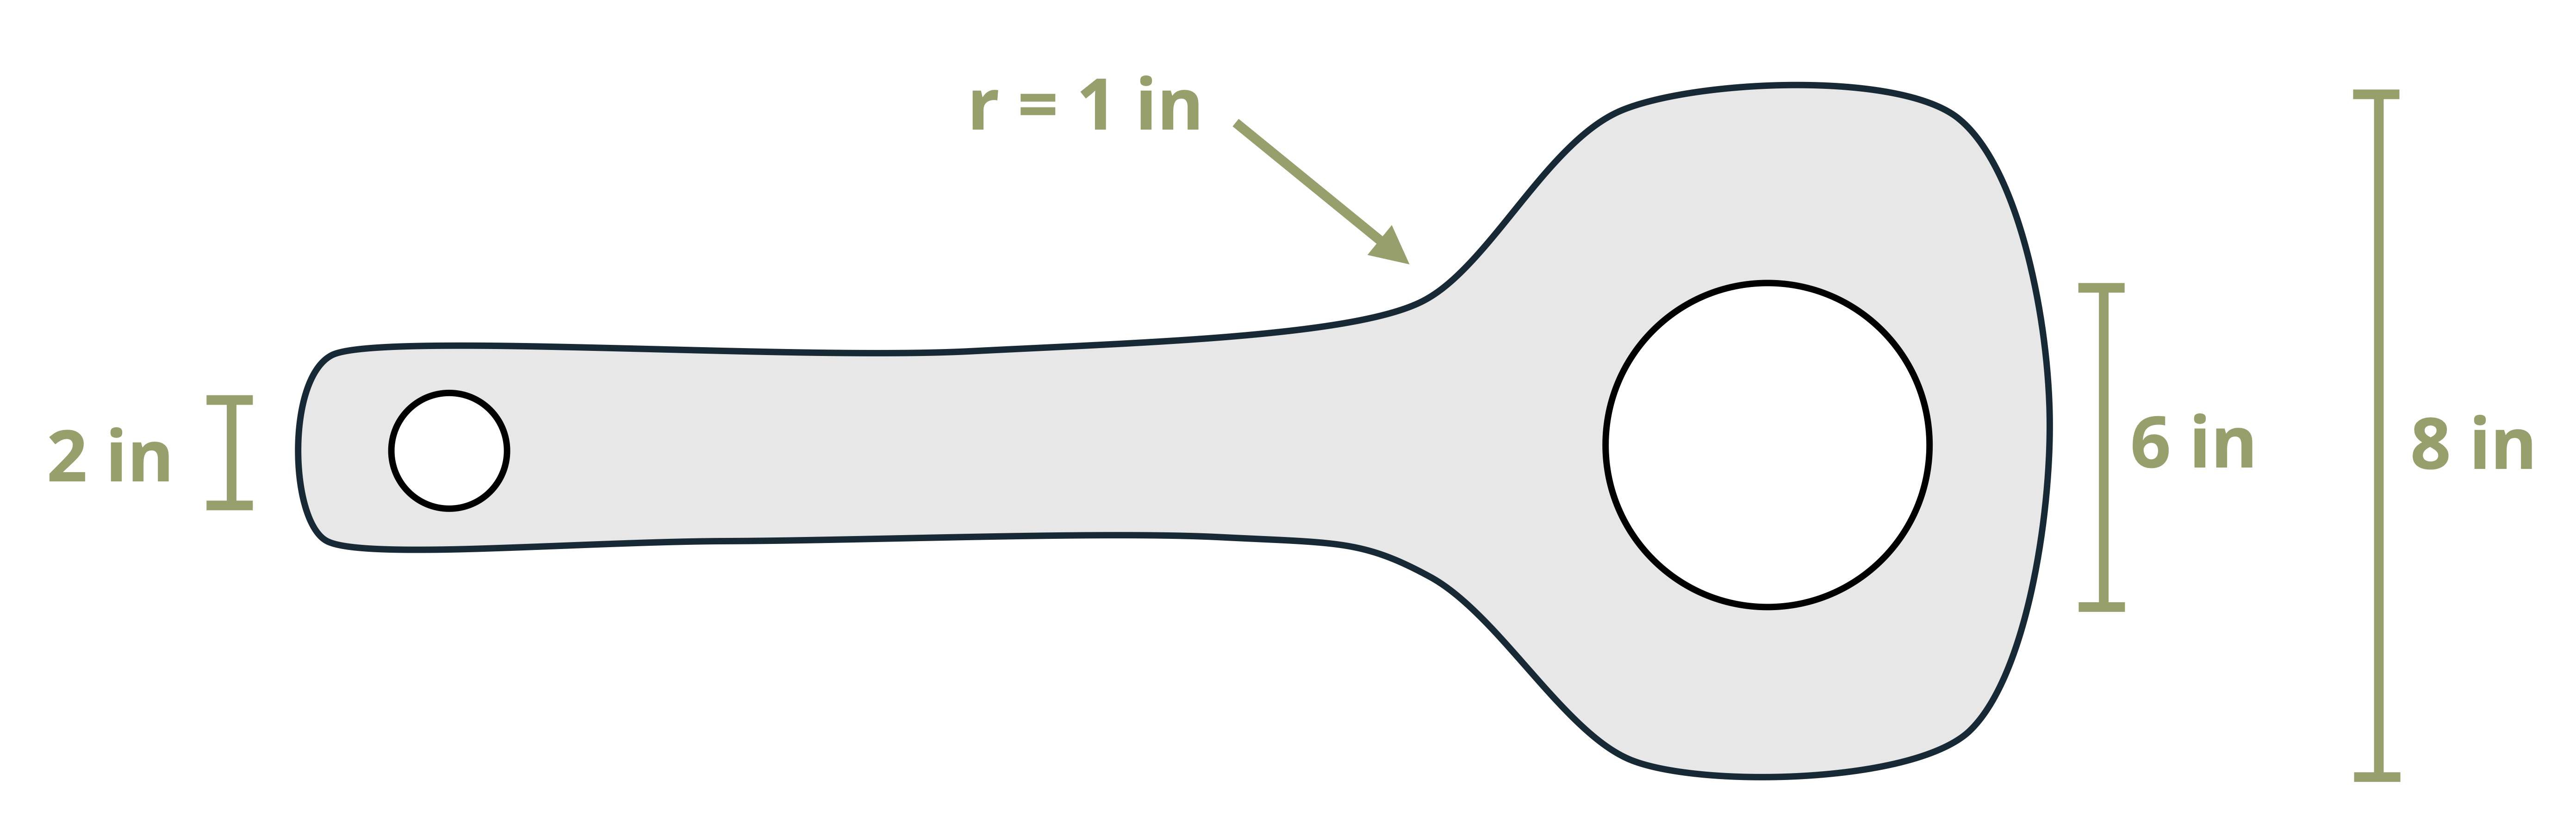
\includegraphics[width=3.78125in,height=\textheight]{images/PNGs/Example 5.2 part 1.png}
\end{center}

\begin{tcolorbox}[enhanced jigsaw, colback=white, colframe=quarto-callout-note-color-frame, leftrule=.75mm, opacitybacktitle=0.6, colbacktitle=quarto-callout-note-color!10!white, arc=.35mm, bottomrule=.15mm, breakable, title={Solution}, left=2mm, titlerule=0mm, toptitle=1mm, toprule=.15mm, opacityback=0, rightrule=.15mm, coltitle=black, bottomtitle=1mm]

The connecting rod has two holes and a fillet. We can start by
determining which of these geometries experiences the largest maximum
stress, in terms of applied load P. For each geometry, calculate the
average normal stress and then use the appropriate stress concentration
curve to determine the maximum normal stress.

For the smaller circle:

\begin{center}
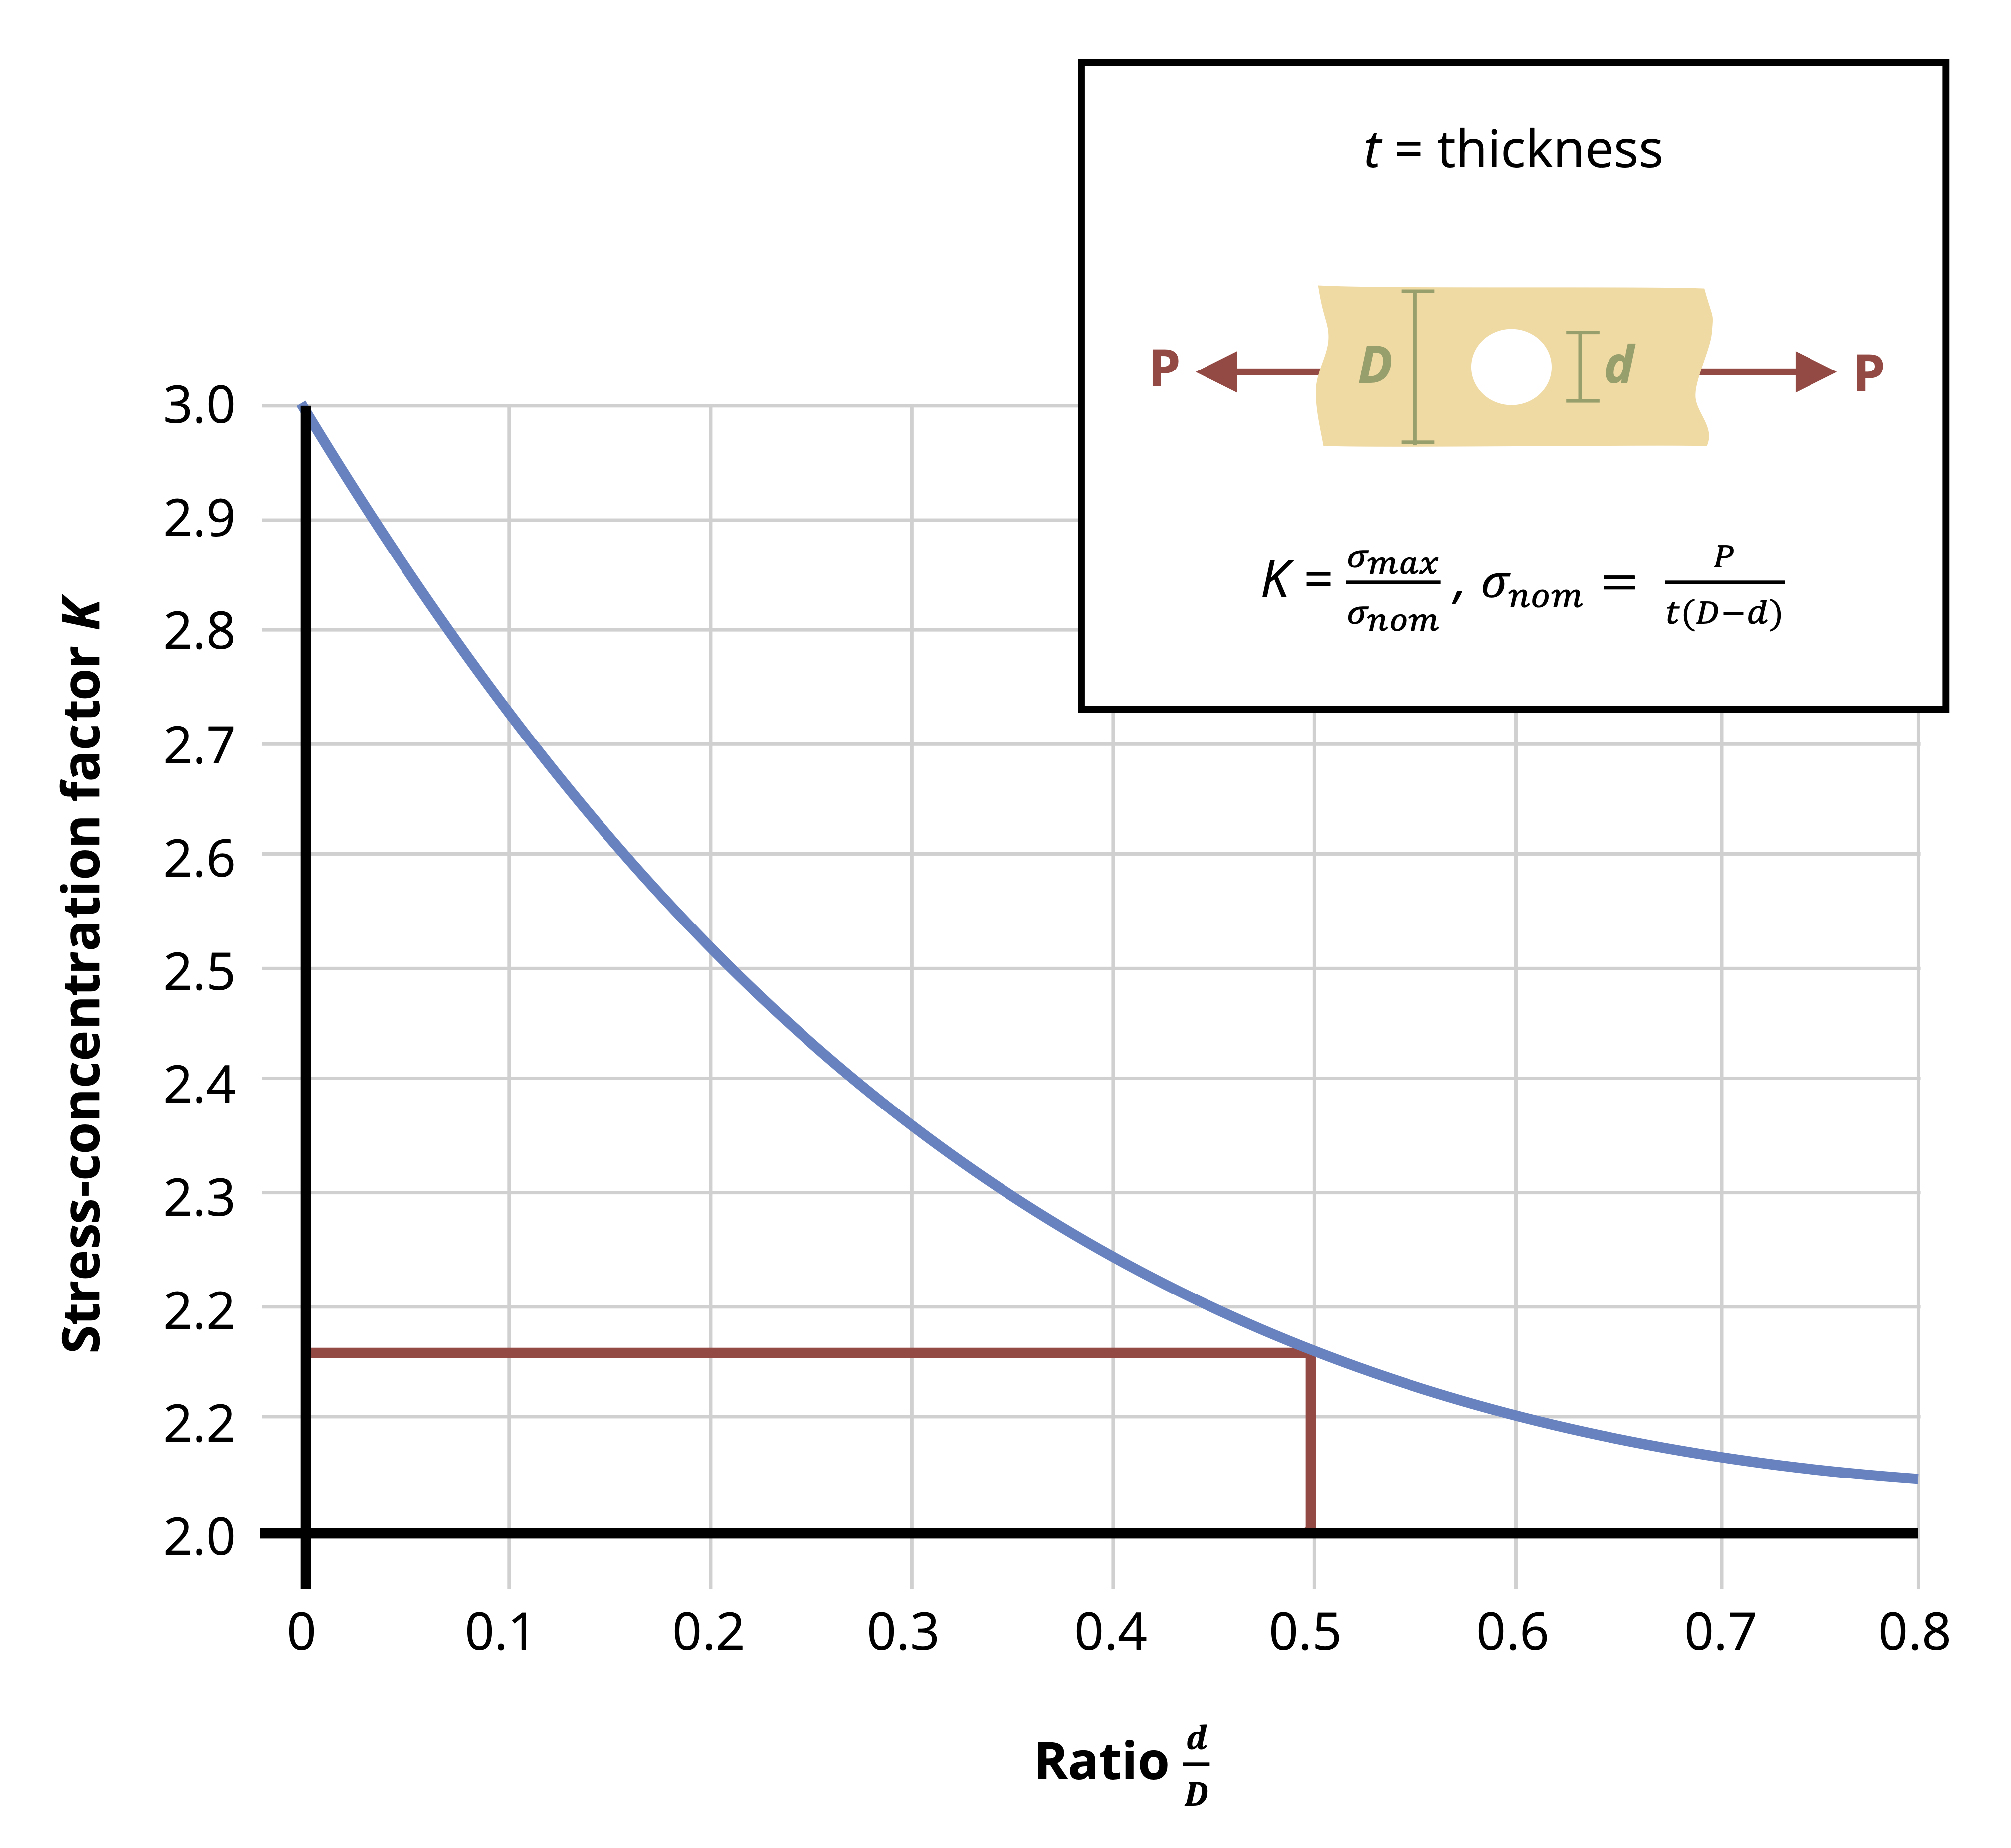
\includegraphics[width=4.23958in,height=\textheight]{images/PNGs/Example 5.2 part 2.png}
\end{center}

\[
\begin{aligned}
& \sigma_{\text {avg }}=\frac{N}{A}=\frac{P}{1 *(4-2)}=\frac{P}{2}=0.5 P \\
& \frac{d}{D}=\frac{2}{4}=0.5 \\
& \mathrm{~K}=2.15 \\
& \sigma_{\max }=K \sigma_{\text {avg }}=2.15 * 0.5 P=1.075 P
\end{aligned}
\]

For the larger circle:

\begin{center}
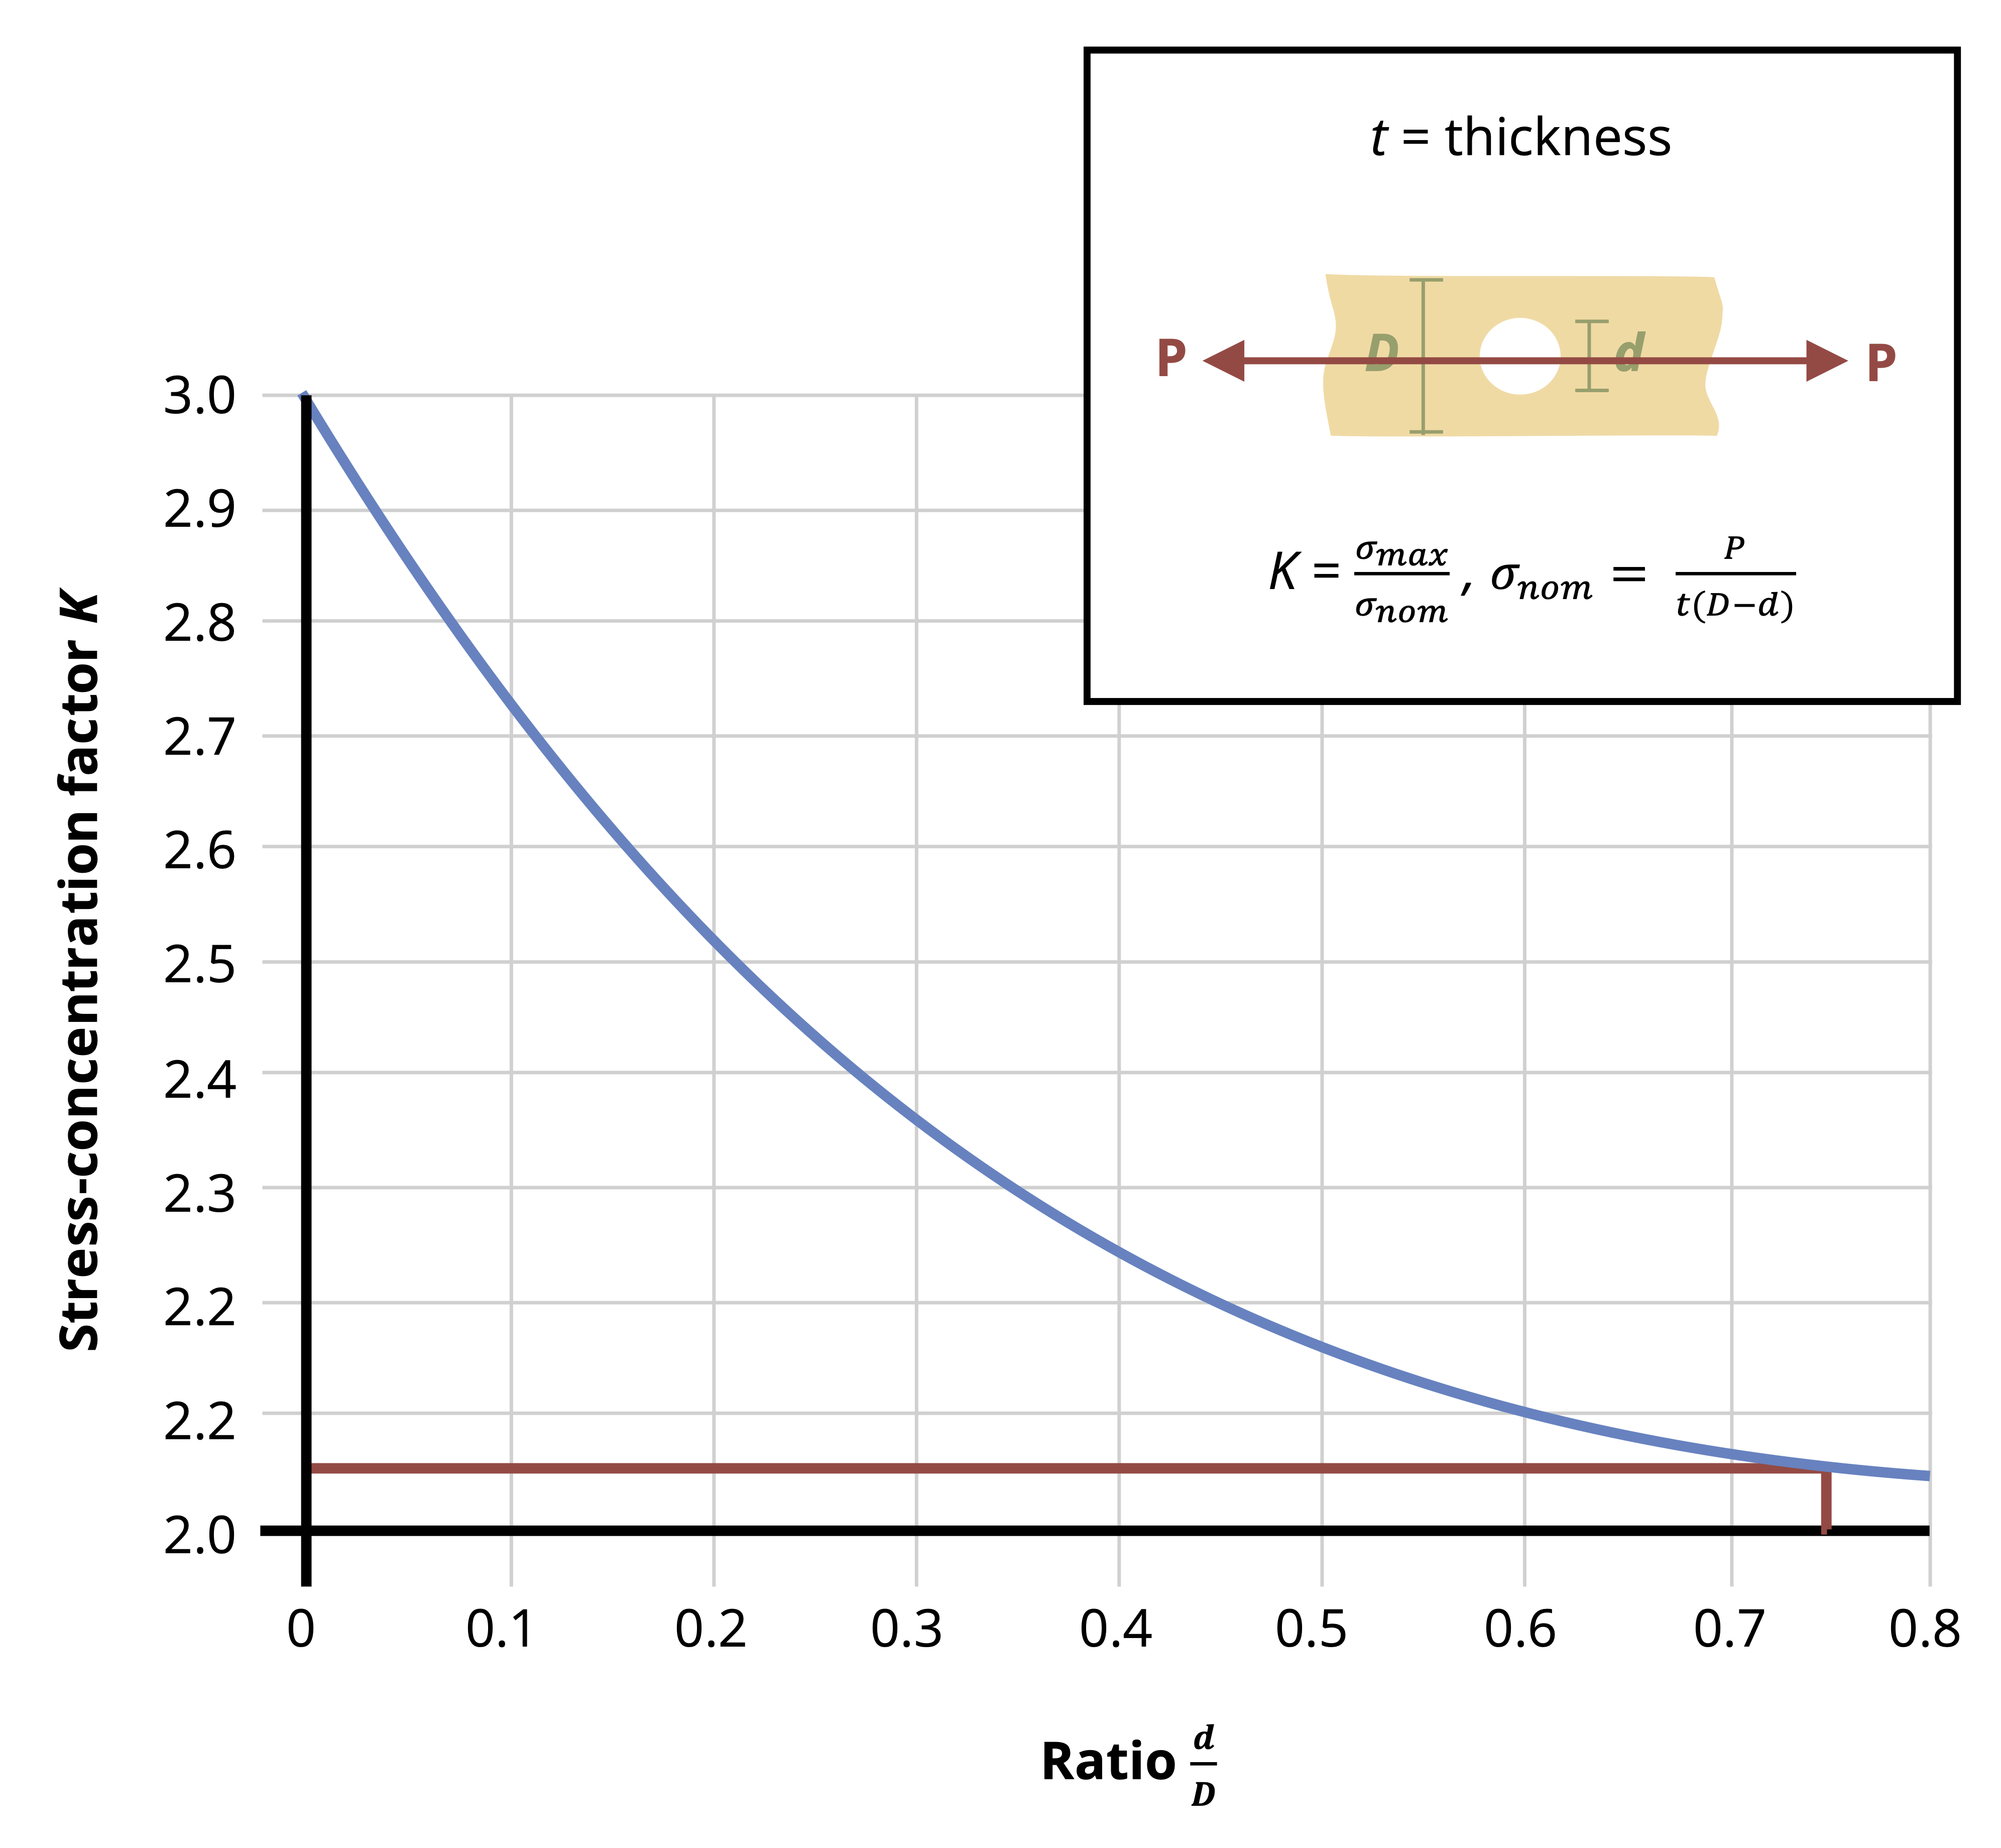
\includegraphics[width=4.54167in,height=\textheight]{images/PNGs/Example 5.2 part 3.png}
\end{center}

\[
\begin{aligned}
& \sigma_{\text {avg }}=\frac{N}{A}=\frac{P}{1 *(8-6)}=\frac{P}{2}=0.5 P \\
& \frac{d}{D}=\frac{6}{8}=0.75 \\
& \mathrm{~K}=2.05 \\
& \sigma_{\text {max }}=K \sigma_{\text {avg }}=2.05 * 0.5 P=1.025 P
\end{aligned}
\]

For the fillet:

\begin{center}
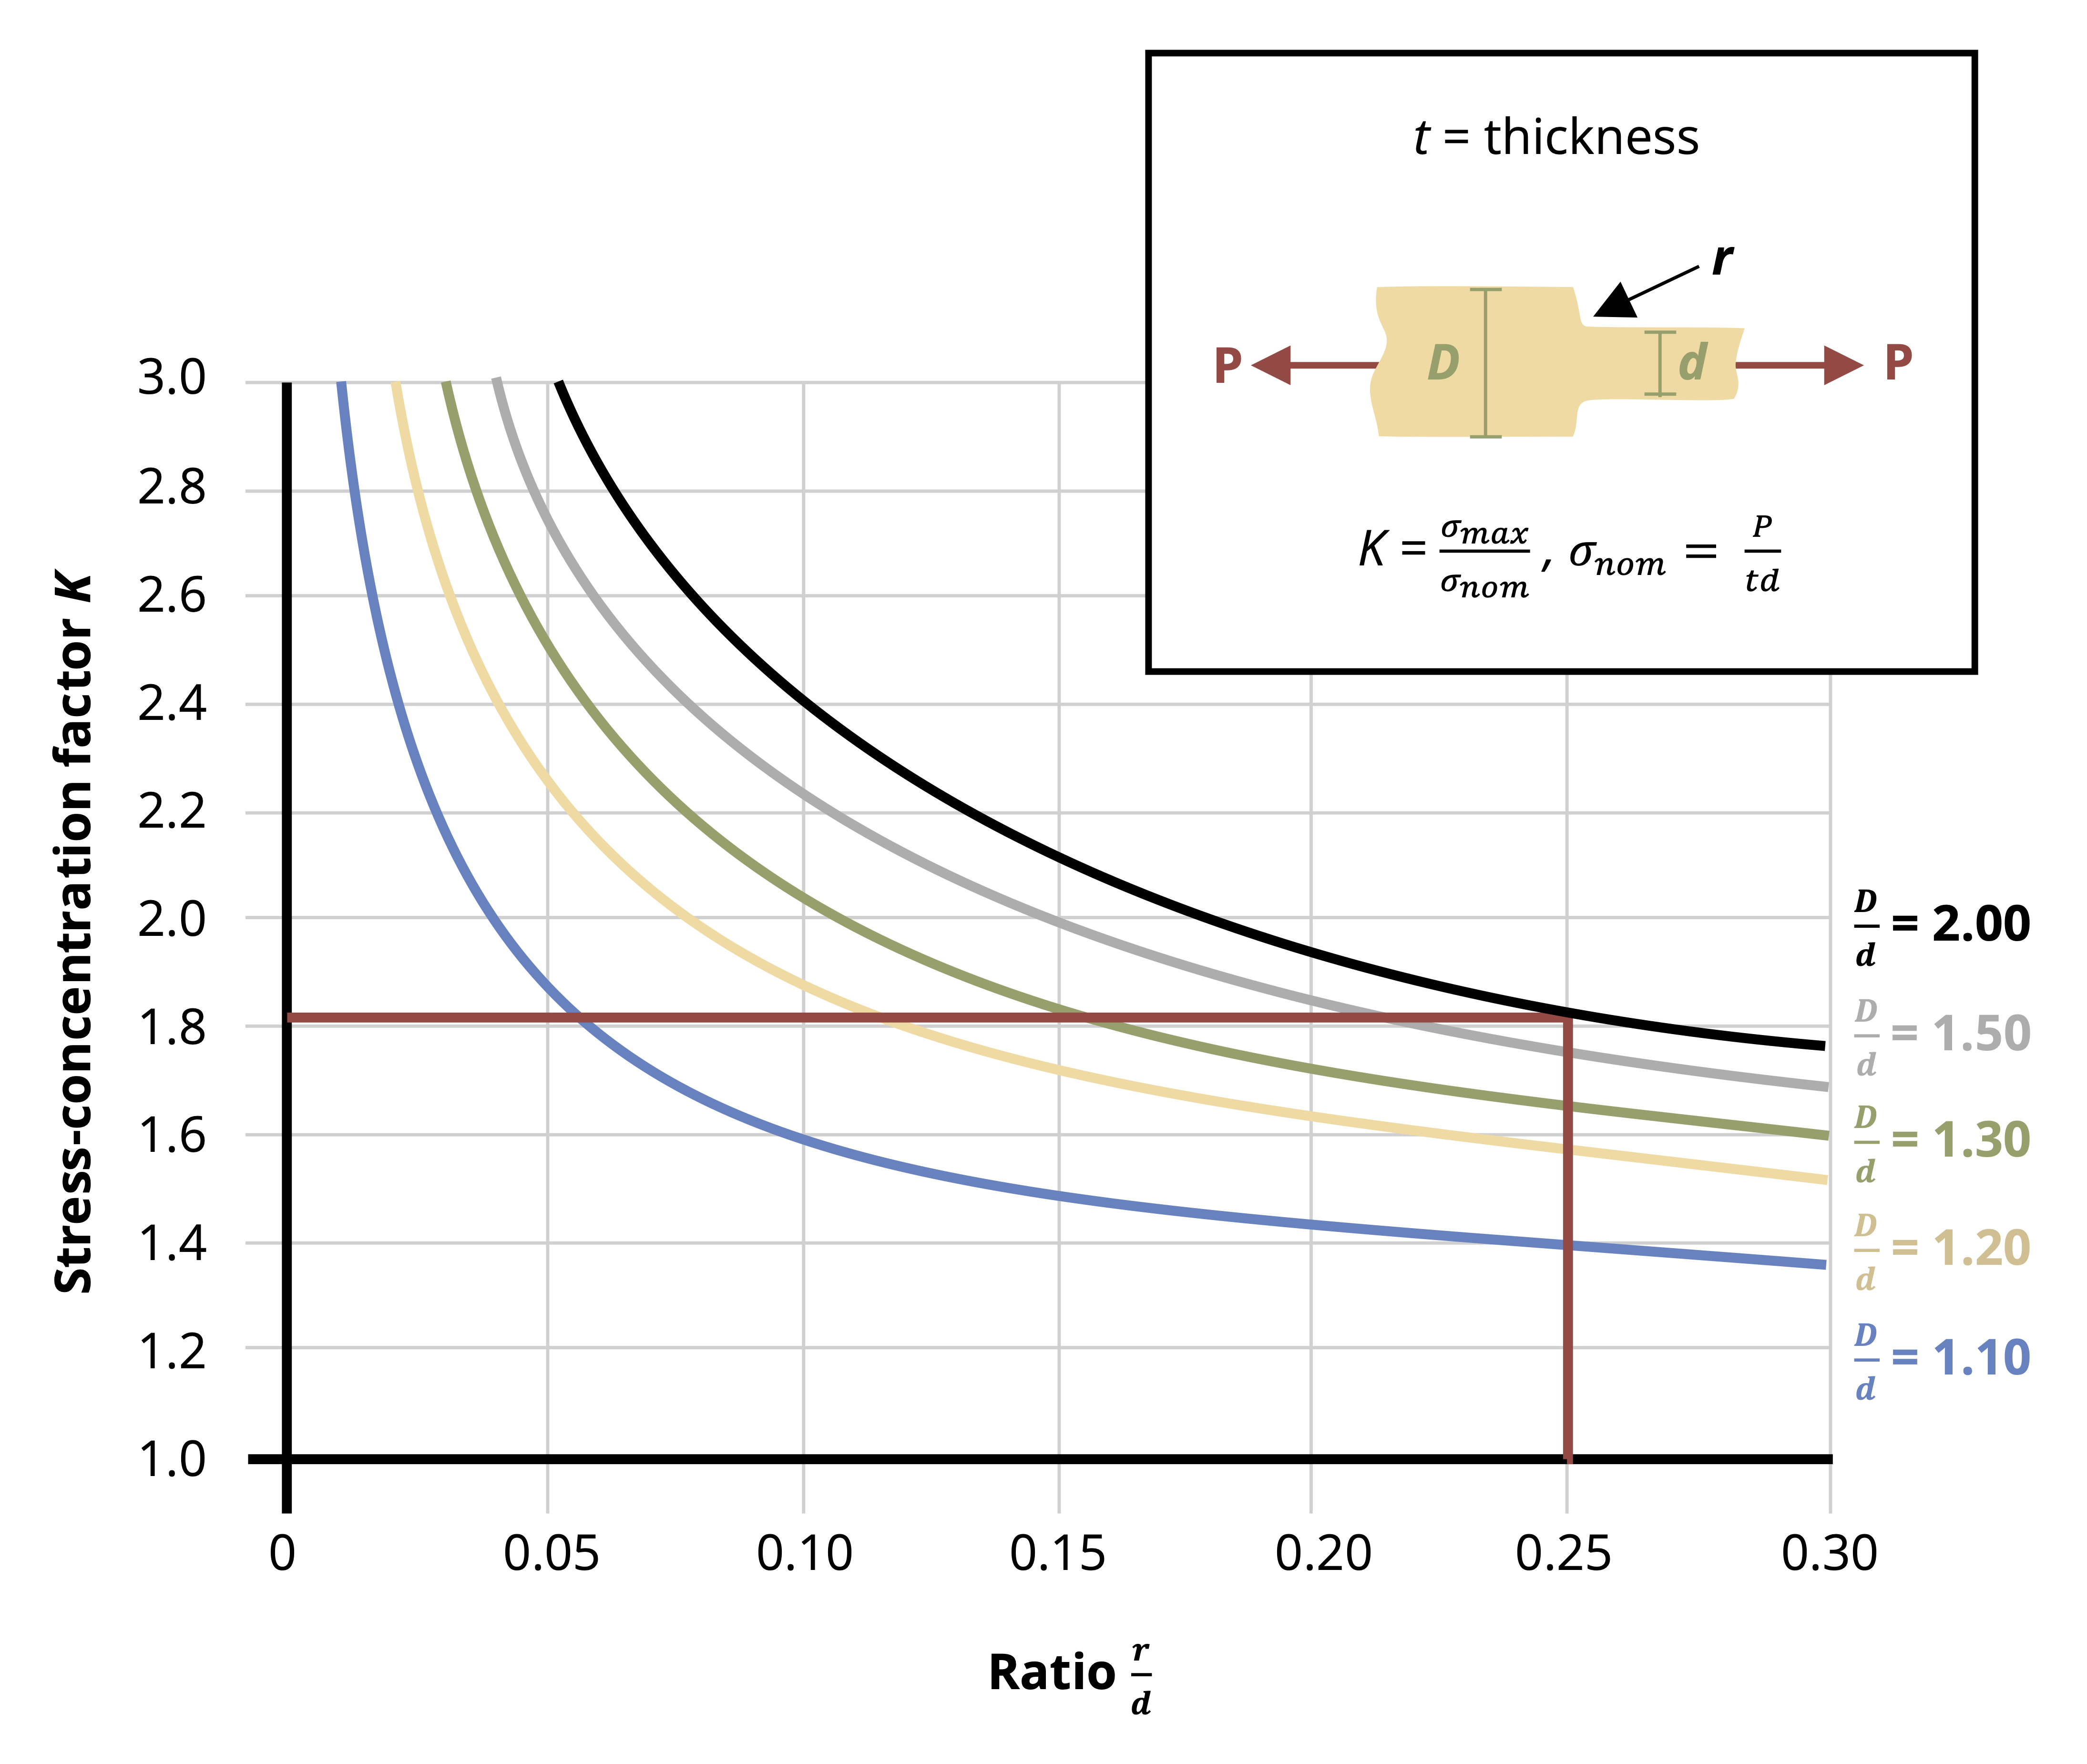
\includegraphics[width=4.38542in,height=\textheight]{images/PNGs/Example 5.2 part 4.png}
\end{center}

\[
\begin{aligned}
& \sigma_{\text {avg }}=\frac{N}{A}=\frac{P}{1 * 4}=\frac{P}{4}=0.25 P \\
& \frac{D}{d}=\frac{8}{4}=2 \\
& \frac{r}{d}=\frac{1}{4}=0.25 \\
& \mathrm{~K}=1.82 \\
& \sigma_{\text {max }}=K \sigma_{\text {avg }}=1.82 * 0.25 P=0.455 P
\end{aligned}
\]

The largest stress is at the small hole, where 𝜎\textsubscript{max} =
1.075\emph{P}.

Since the maximum allowable stress is 40 ksi,
\(40=1.075 P \rightarrow P=\frac{40}{1.075}=37.2\) kips.

\end{tcolorbox}

\end{tcolorbox}

\begin{tcolorbox}[enhanced jigsaw, colback=white, colframe=quarto-callout-note-color-frame, leftrule=.75mm, opacitybacktitle=0.6, colbacktitle=quarto-callout-note-color!10!white, arc=.35mm, bottomrule=.15mm, breakable, title={Step-by-step: Stress concentrations}, left=2mm, titlerule=0mm, toptitle=1mm, toprule=.15mm, opacityback=0, rightrule=.15mm, coltitle=black, bottomtitle=1mm]

\begin{enumerate}
\def\labelenumi{\arabic{enumi}.}
\item
  Calculate the average normal stress using
  \(\sigma_{\text {avg }}=\frac{N}{A}\). Do this at the hole or at the
  thinner section of the fillet.
\item
  Use the appropriate stress concentration curve to determine the stress
  concentration factor, K, for the given geometry.
\item
  Calculate the maximum stress from
  \(\sigma_{\text {max }}=K \sigma_{\text {avg }}\)
\end{enumerate}

\end{tcolorbox}

\section{Axial Deformation}\label{axial-deformation}

Click to expand

Consider a simple bar of uniform cross-section subjected to an axial
force (Figure 5.6).

\begin{figure}[H]

{\centering 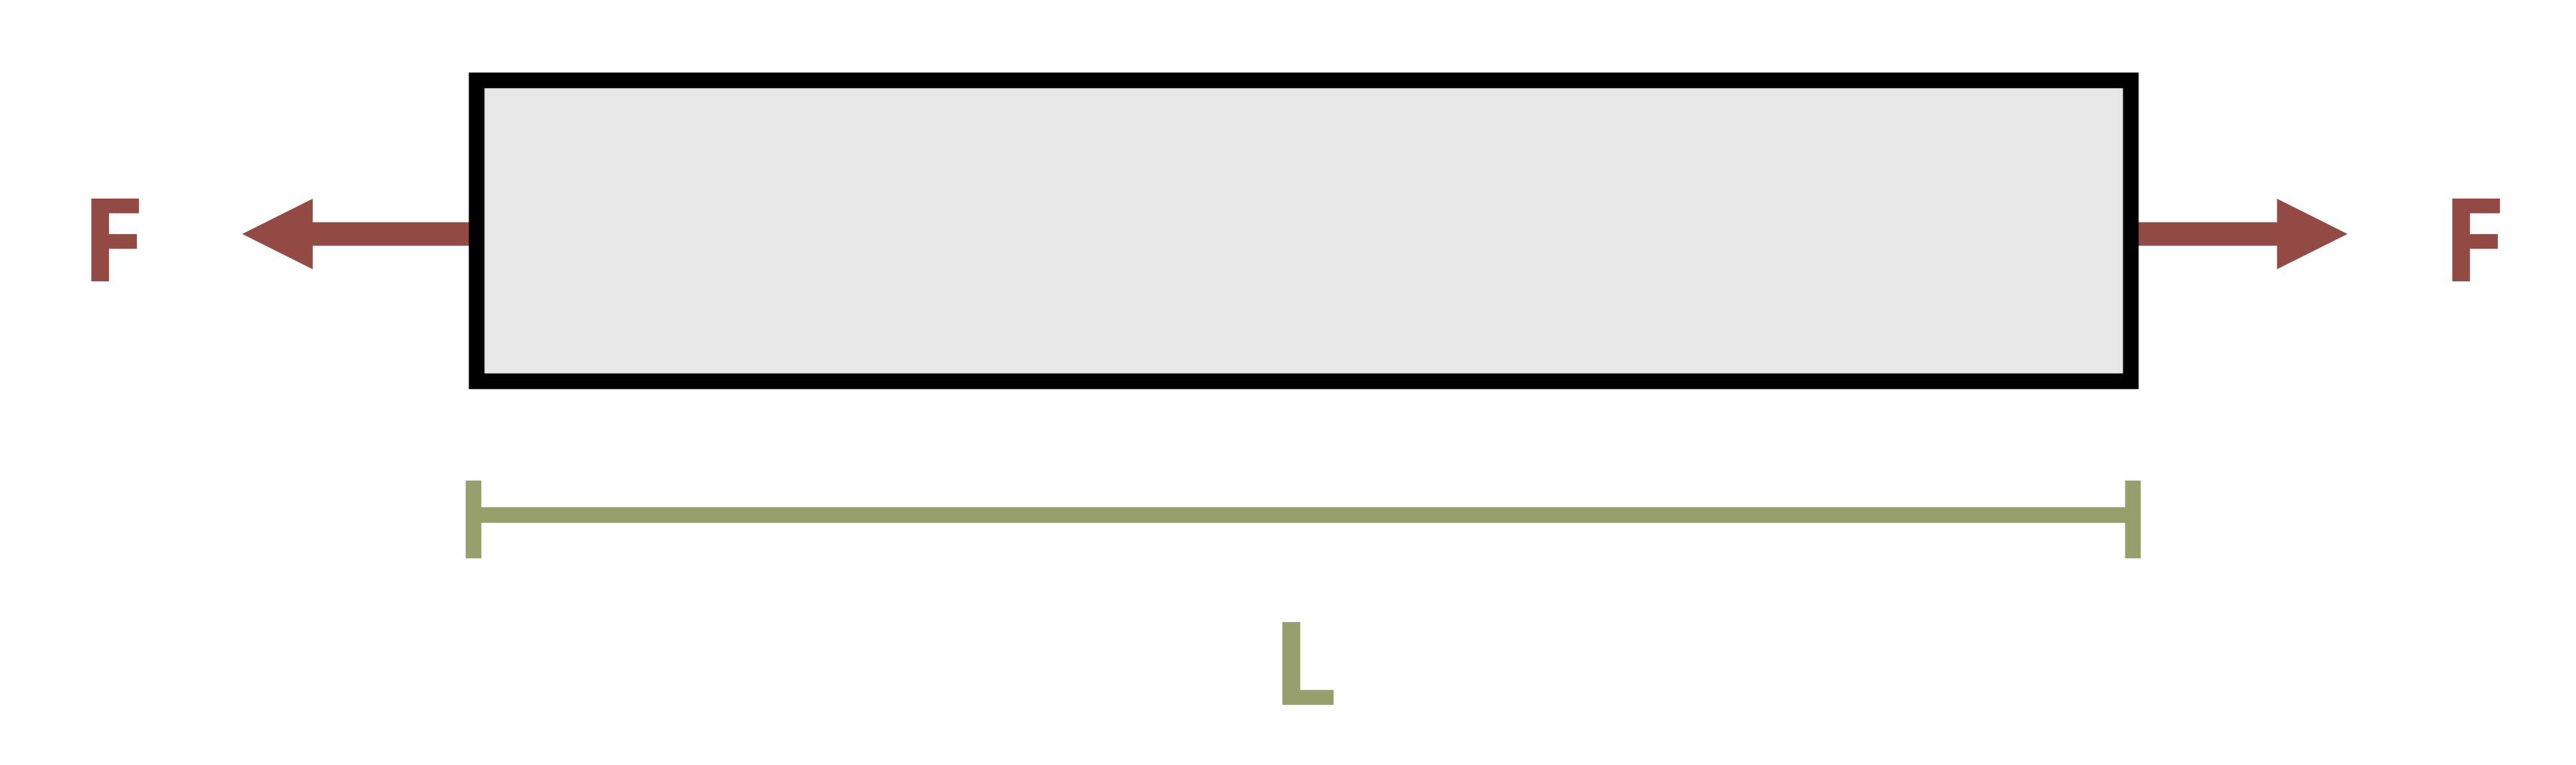
\includegraphics[width=3.48958in,height=\textheight]{images/PNGs/Figure 5.6.png}

}

\caption{Figure 5.6: A bar of uniform cross-section, A, and length, L,
subjected to axial load, F.}

\end{figure}%

Assuming elastic behavior, we have equations for stress and strain, as
well as Hooke's law which relates the two equations:

\[
\begin{aligned} & \sigma=\frac{F}{A} \\ & \varepsilon_{\text {long }}=\frac{\Delta L}{L} \\ & \sigma=E \varepsilon_{\text {long }}\end{aligned}\]

Replacing the stress and strain terms in Hooke's law:

\[
\frac{F}{A}=E \frac{\Delta L}{L}\]

Rearranging:

\[
\Delta L=\frac{F L}{A E}\]

\emph{where}

\emph{ΔL = Change in length {[}m, in.{]}}

\emph{F = internal axial load {[}N, lb{]}}

\emph{L = Original length {[}m, in.{]}\$}

\emph{A = Cross-sectional area {[}m\textsuperscript{2},
in.\textsuperscript{2}{]}}

\emph{E = Elastic modulus {[}Pa, psi{]}}

This equation can be used to directly find the change in length of an
object subjected to an axial load.

In practice, there may be multiple axial loads applied to the bar. The
cross-sectional area may change at different points along the bar, or
perhaps there could be different materials with different elastic moduli
connected in series to form the bar. In any of these cases we can split
the bar into sections where each section has a constant F, A, and E. We
can calculate the change in length of each section separately and sum
them to find the total. See Example 5.3 for a problem involving multiple
segments of a bar.

\[
\Delta L=\sum \frac{F L}{A E}\]

\begin{tcolorbox}[enhanced jigsaw, colback=white, colframe=quarto-callout-note-color-frame, leftrule=.75mm, opacitybacktitle=0.6, colbacktitle=quarto-callout-note-color!10!white, arc=.35mm, bottomrule=.15mm, breakable, title={Example 5.3: Axial change in length problem with different loads, areas,
and materials}, left=2mm, titlerule=0mm, toptitle=1mm, toprule=.15mm, opacityback=0, rightrule=.15mm, coltitle=black, bottomtitle=1mm]

A component is made by welding together 2 circular rods. Rod (1) is made
of steel (E = 29 x 10\textsuperscript{6} psi) and is hollow, with an
outer diameter of 4 in. and an inner diameter of 2 in. Rod (2) is made
of copper (E = 17 x 10\textsuperscript{6} psi) and is solid, with a
diameter of 5 in. If the component is subjected to the axial loads
shown, determine the total deformation of the component.

\begin{center}
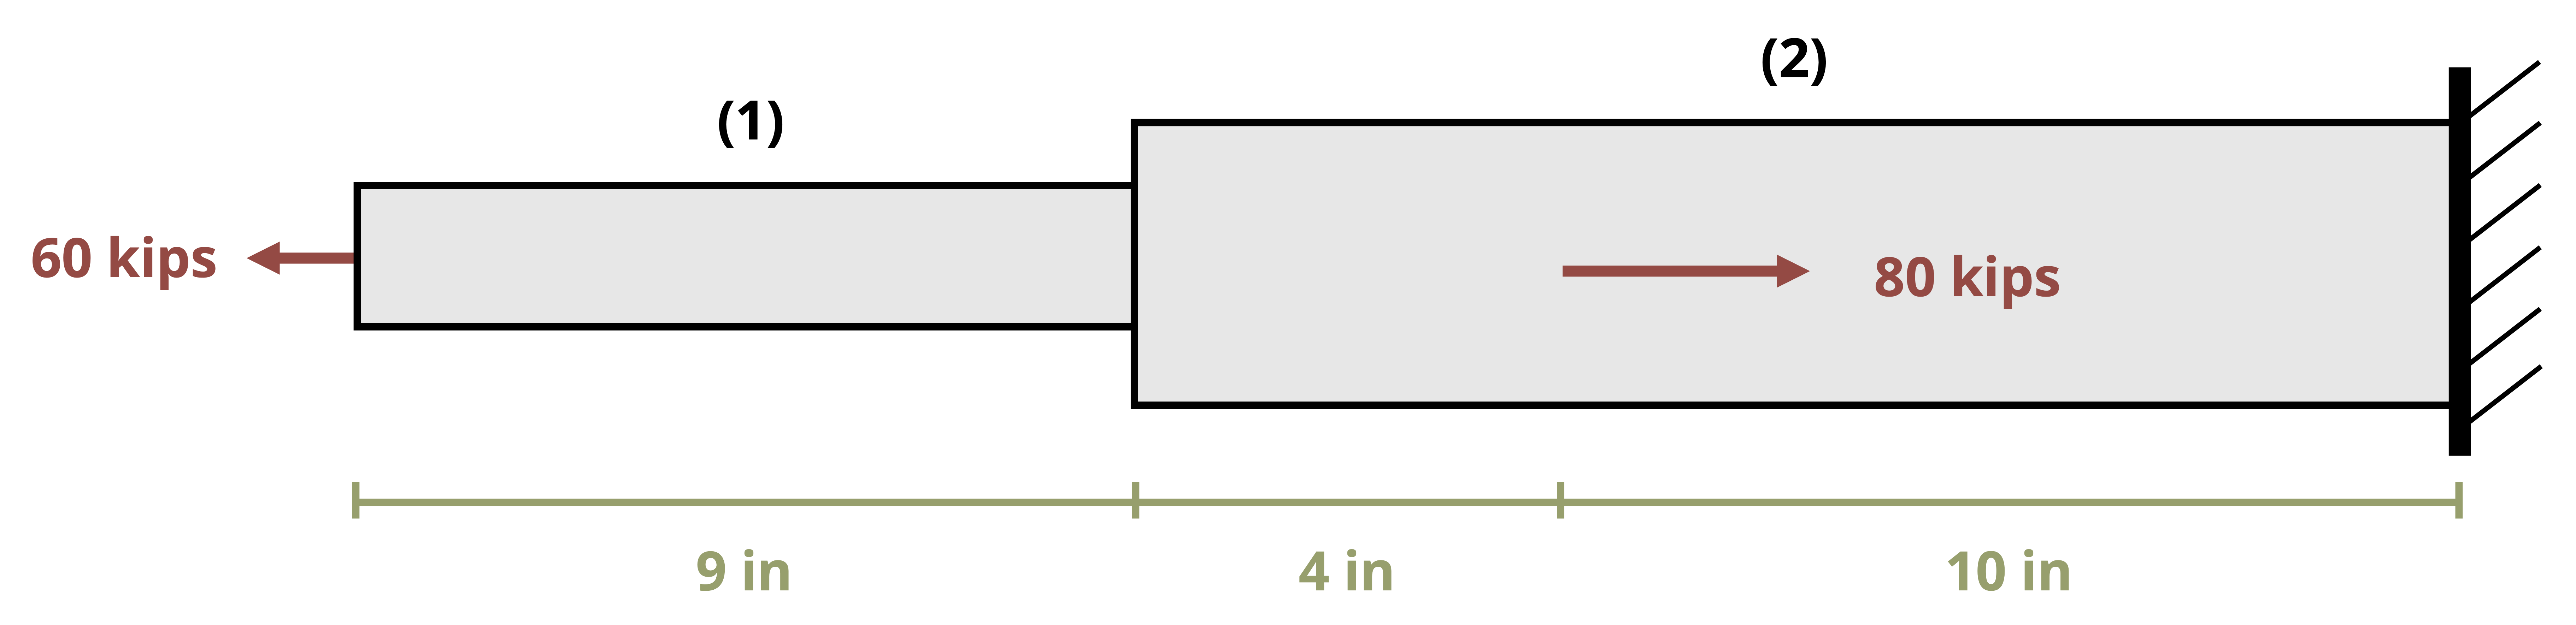
\includegraphics{images/PNGs/Example 5.3 part 1.png}
\end{center}

\begin{tcolorbox}[enhanced jigsaw, colback=white, colframe=quarto-callout-note-color-frame, leftrule=.75mm, opacitybacktitle=0.6, colbacktitle=quarto-callout-note-color!10!white, arc=.35mm, bottomrule=.15mm, breakable, title={Solution}, left=2mm, titlerule=0mm, toptitle=1mm, toprule=.15mm, opacityback=0, rightrule=.15mm, coltitle=black, bottomtitle=1mm]

We can find the change in length of the component using
\(\Delta L=\sum \frac{F L}{A E}\).

First, break the component into three segments and determine the
internal load in each segment. The first segment covers the 9-inch steel
rod. After the first 9 inches of the component, both the cross-sectional
area and elastic modulus change so a second segment is needed. This
segment covers the next 4 inches. At this point the loading changes, so
a third segment is required to cover the final 10 inches of the
component.

\begin{center}
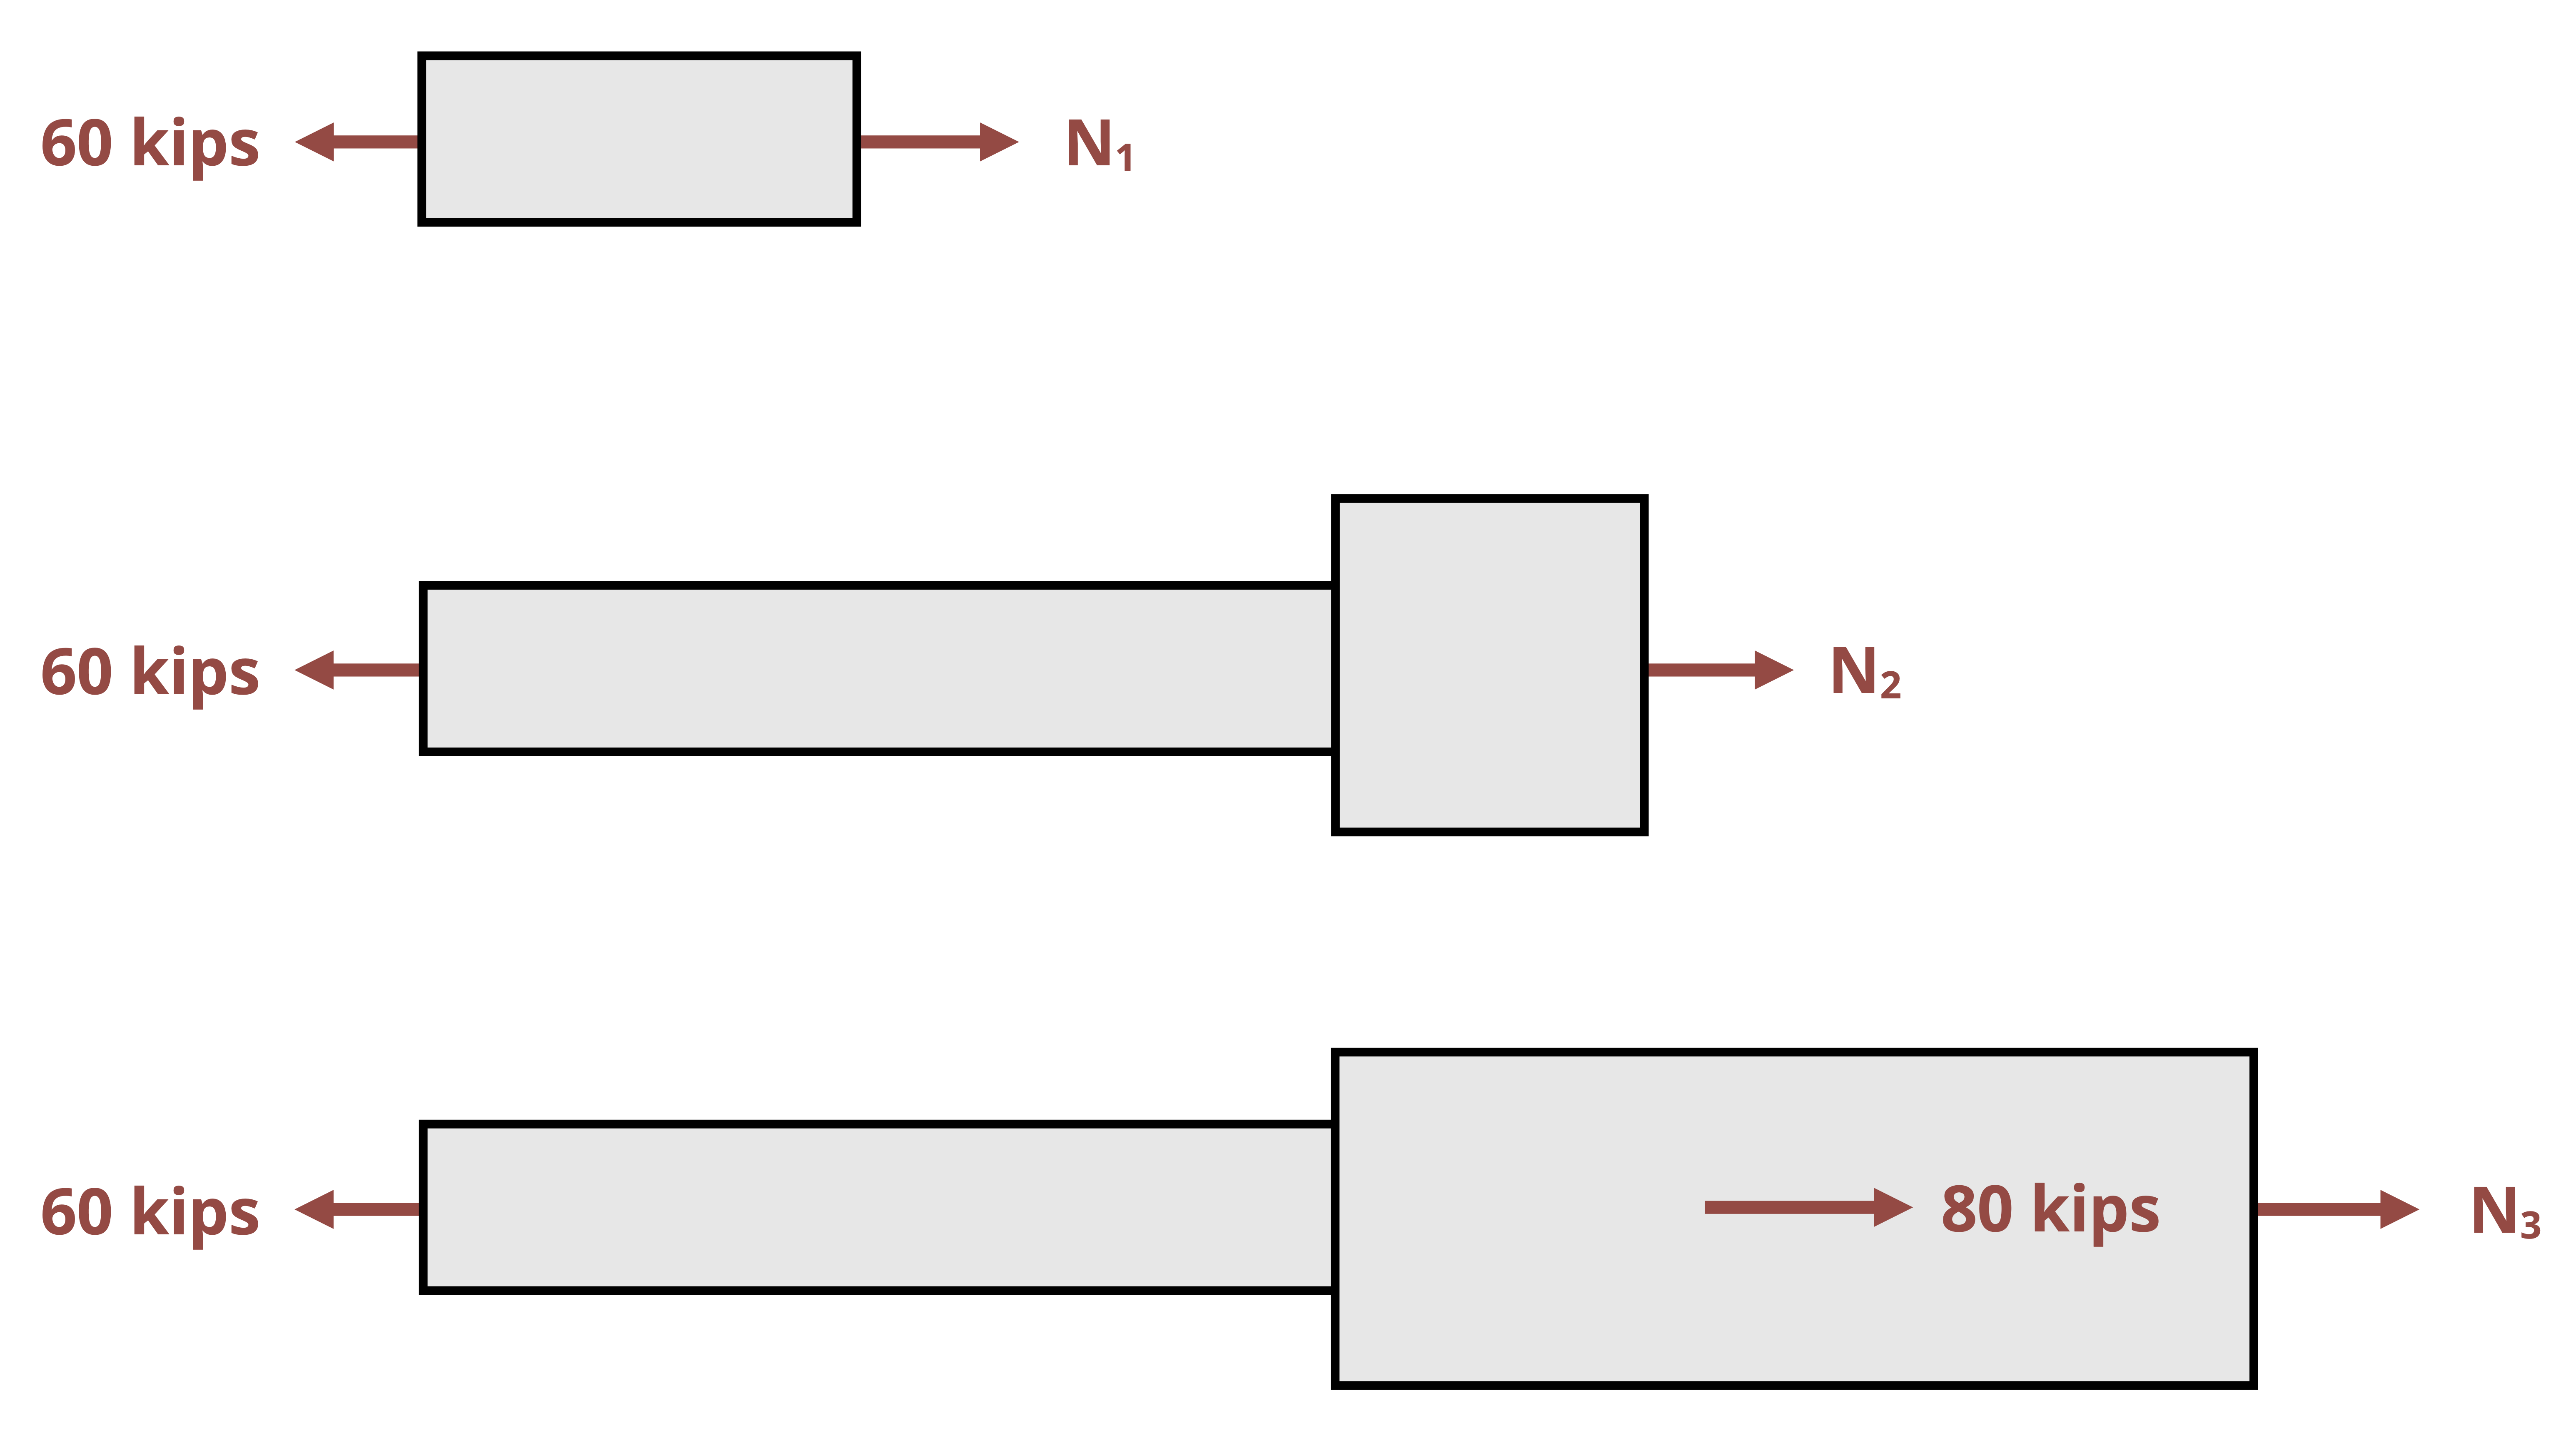
\includegraphics[width=4.625in,height=\textheight]{images/PNGs/Example 5.3 part 2.png}
\end{center}

\[
\begin{gathered}
N_1=N_2=60 \mathrm{kips} \\
N_3=-20 \mathrm{kips}
\end{gathered}
\]

Now calculate the deformation of each segment. Be sure to use the
appropriate dimensions and material properties for each segment.

Cross-sectional areas:

\[
\begin{gathered}
A_1=\pi *\left(2^2-1^2\right)=9.42 i n .{ }^2 \\
A_2=\pi *\left(2.5^2\right)=19.6 i n .{ }^2
\end{gathered}
\]

Deformation of segment 1:

\[
\Delta L_1=\frac{60000 * 9}{9.42 * 29 \times 10^6}=0.00198 \mathrm{in.}
\]

Deformation of segment 2:

\[
\Delta L_2=\frac{60000 * 4}{19.6 * 17 \times 10^6}=0.000719 \mathrm{in} .
\]

Deformation of segment 3:

\[
\Delta L_3=\frac{-20000 * 10}{19.6 * 17 \times 10^6}=-0.000599 \mathrm{in.}
\]

Note that segment 3 is in compression and so gets shorter, while
segments 1 and 2 are in tension and so get longer. The total deformation
in the component is simply the sum of these three deformations.

\[
\Delta L=0.00198+0.000719-0.000599=0.0021 \mathrm{in} .
\]

\end{tcolorbox}

\end{tcolorbox}

\begin{tcolorbox}[enhanced jigsaw, colback=white, colframe=quarto-callout-note-color-frame, leftrule=.75mm, opacitybacktitle=0.6, colbacktitle=quarto-callout-note-color!10!white, arc=.35mm, bottomrule=.15mm, breakable, title={Step-by-step: Axial deformation}, left=2mm, titlerule=0mm, toptitle=1mm, toprule=.15mm, opacityback=0, rightrule=.15mm, coltitle=black, bottomtitle=1mm]

\begin{enumerate}
\def\labelenumi{\arabic{enumi}.}
\item
  Split the bar into sections of constant F, A, and E. Any time any of
  these terms changes, begin a new section.
\item
  Determine the length of each section.
\item
  Calculate the change in length of each section using
  \(\Delta L=\frac{F L}{A E}\).
\item
  Determine the total change in length by summing the change in length
  of each section. Remember some sections may elongate while others
  contract.
\end{enumerate}

\end{tcolorbox}

\section{Deformation in Series of
Bars}\label{deformation-in-series-of-bars}

Click to expand

Sometimes a structure will have more than one axially loaded member. In
such cases there are multiple bars that will experience a change in
length and the amount of deformation won't necessarily be the same in
each member. The deformable members are generally connected by a rigid
(nondeformable) beam. These problems generally involve a little geometry
alongside our deformation equation (Figure 5.6).

\begin{figure}[H]

{\centering 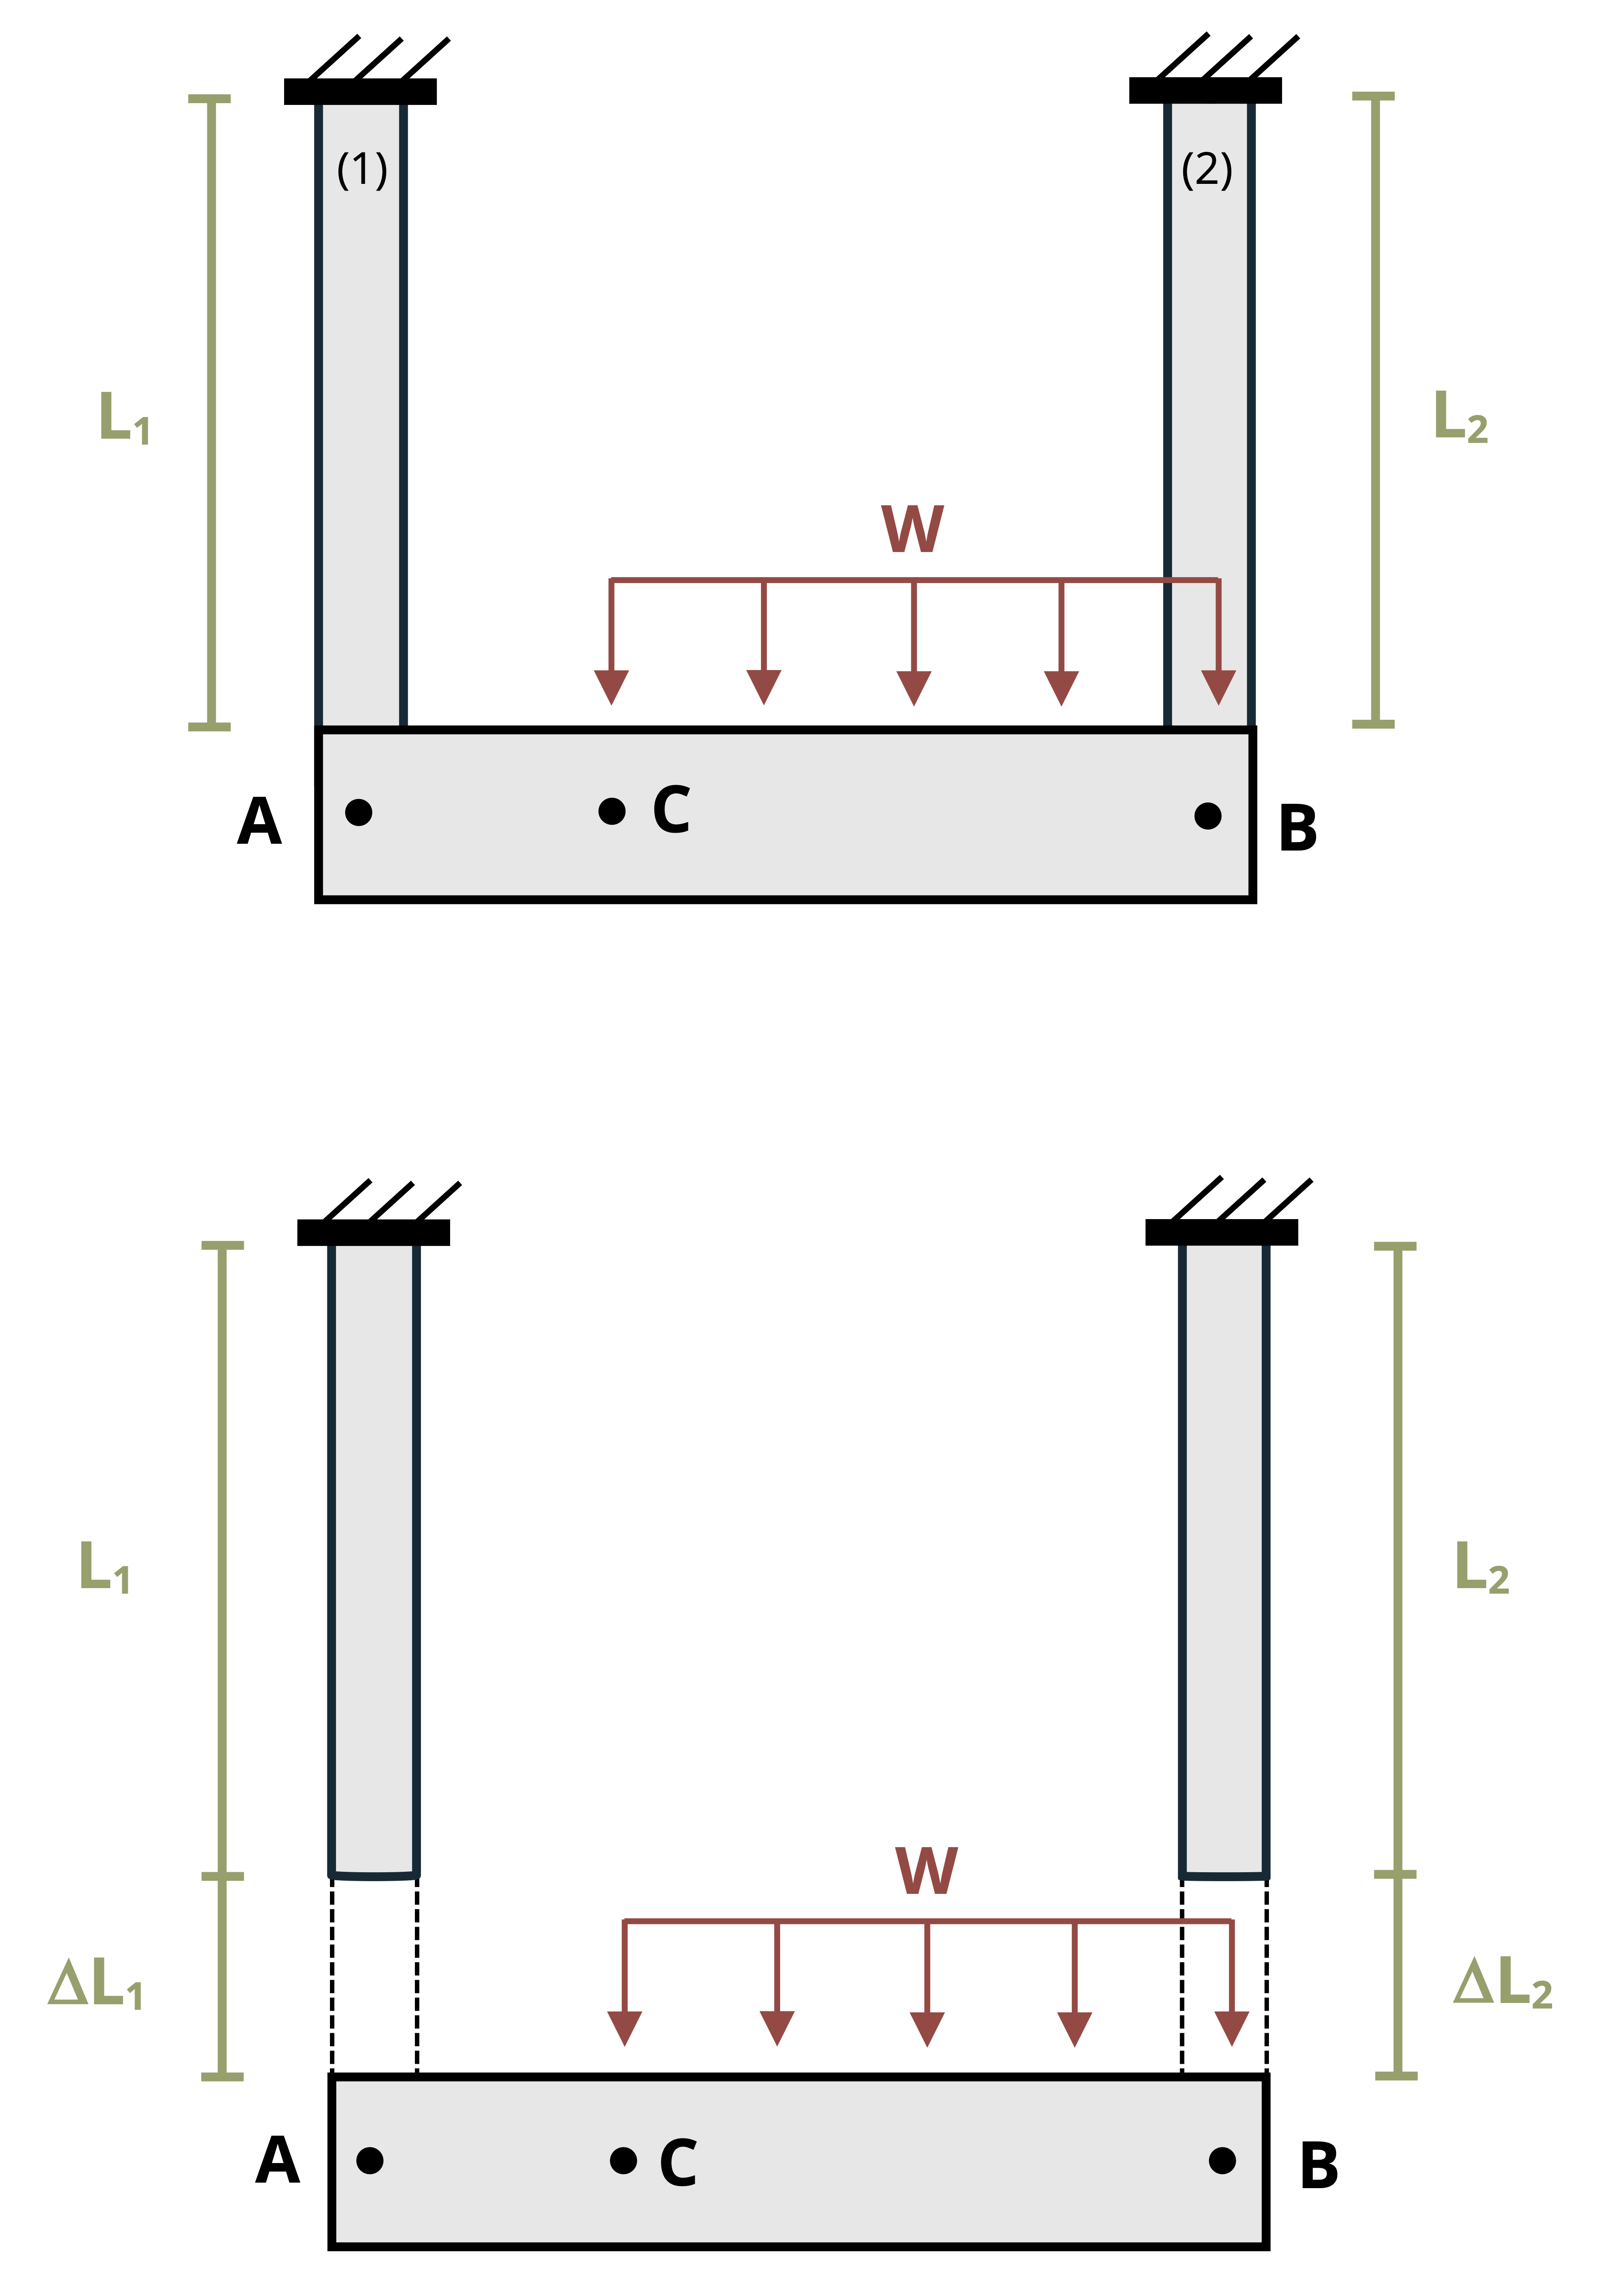
\includegraphics[width=3.75in,height=\textheight]{images/PNGs/Figure 5.7.png}

}

\caption{Figure 5.6: Rigid beam AB is attached to deformable poles 1 and
2. The poles may deform different amounts so point A is displaced by
amount ΔL\textsubscript{1}, point B by amount ΔL\textsubscript{2}, and
point C by an amount in between these two values.}

\end{figure}%

By identifying the force in each member through equilibrium, we may
calculate the deformation of each member separately using:

\[
\Delta L=\frac{F L}{A E}\]

Once the change in length of each member is known, we can find the
displacement at different points on the rigid beam through simple
geometry of the rigid beam (Figure 5.7). This process is demonstrated in
Example 5.4.

\begin{figure}[H]

{\centering 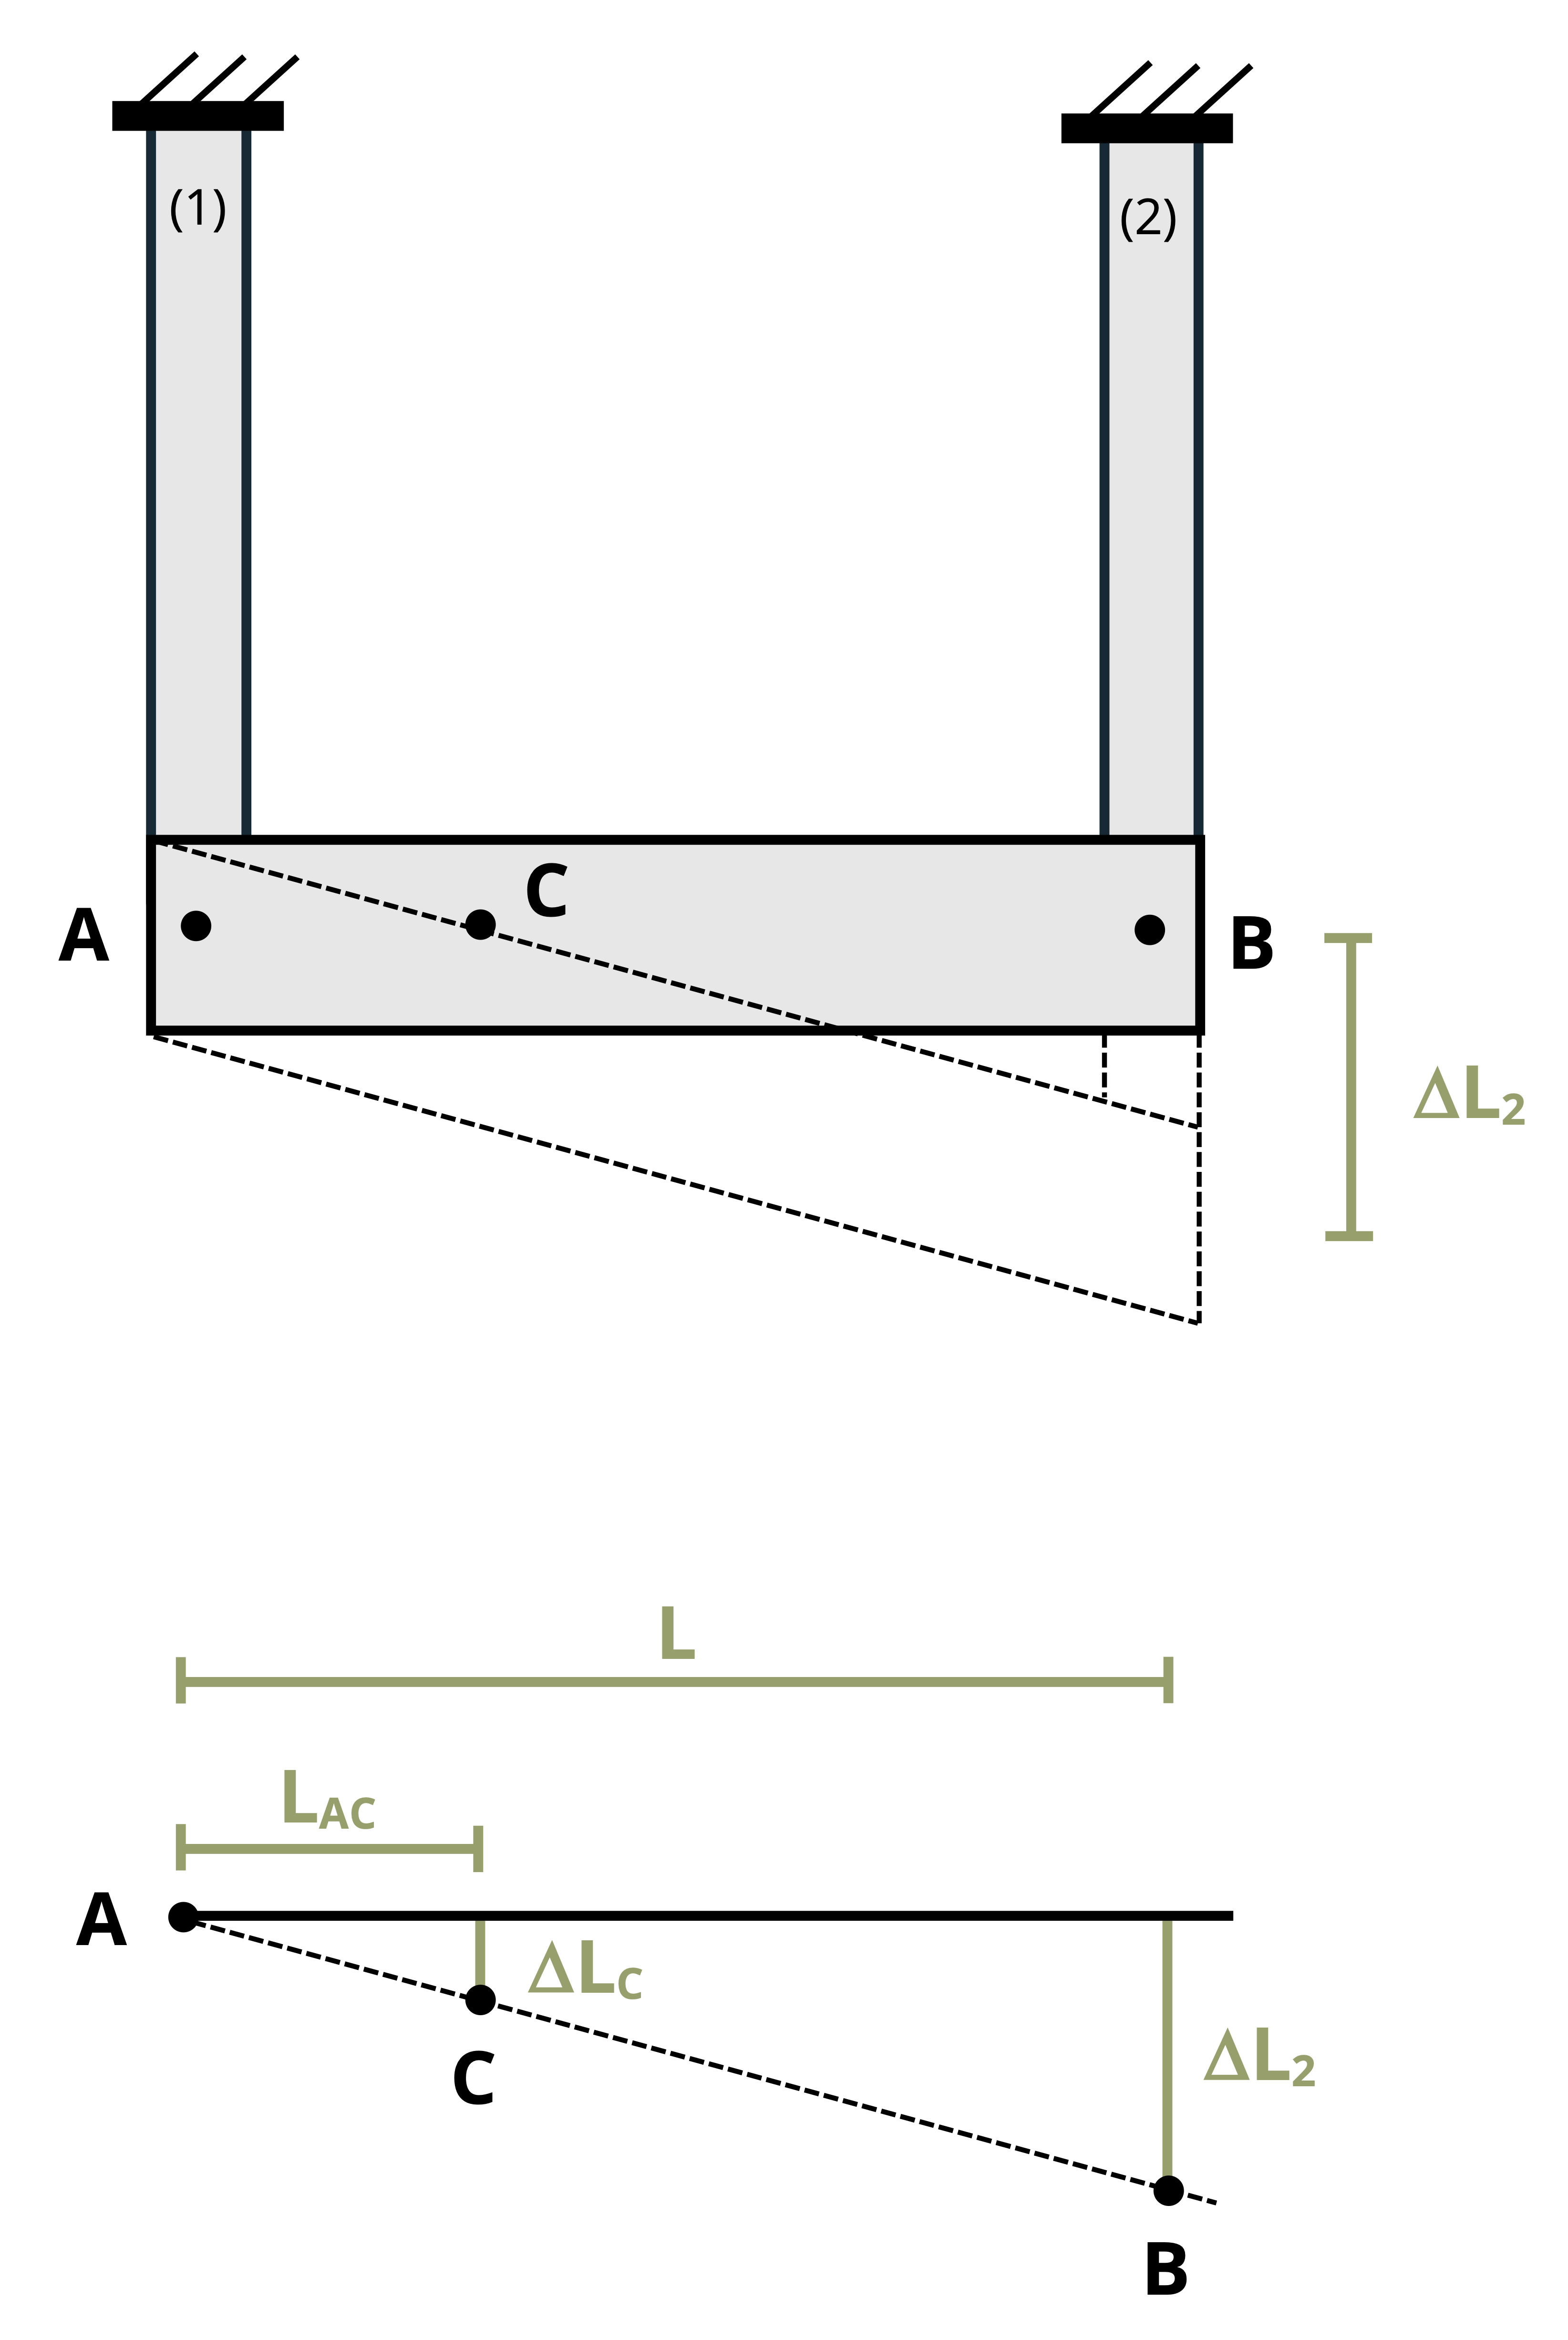
\includegraphics[width=3.42708in,height=\textheight]{images/PNGs/Figure 5.8.png}

}

\caption{Figure 5.7: Beam deflection in the case where only bar 2
deforms. Point B will deflect downward by amount ΔL\textsubscript{2}.
The deflection at point C can be determined through geometry.}

\end{figure}%

The deflection of point C will be somewhere between the deflection at A
and the deflection at B. Assuming there is no deflection at A and
assuming that the deflections (and therefore the angle at A) are small,
we can use similar triangles to find:

\[
\frac{\Delta L_C}{L_{A C}}=\frac{\Delta L_2}{L} \rightarrow \Delta L_C=\Delta L_2 \frac{L_{A C}}{L}\]

If there is a deflection at point A (Figure 5.8) this simply becomes:

\[
\Delta L_C=\Delta L_1+\left(\Delta L_2-\Delta L_1\right) \frac{L_{A C}}{L}\]

\begin{figure}[H]

{\centering 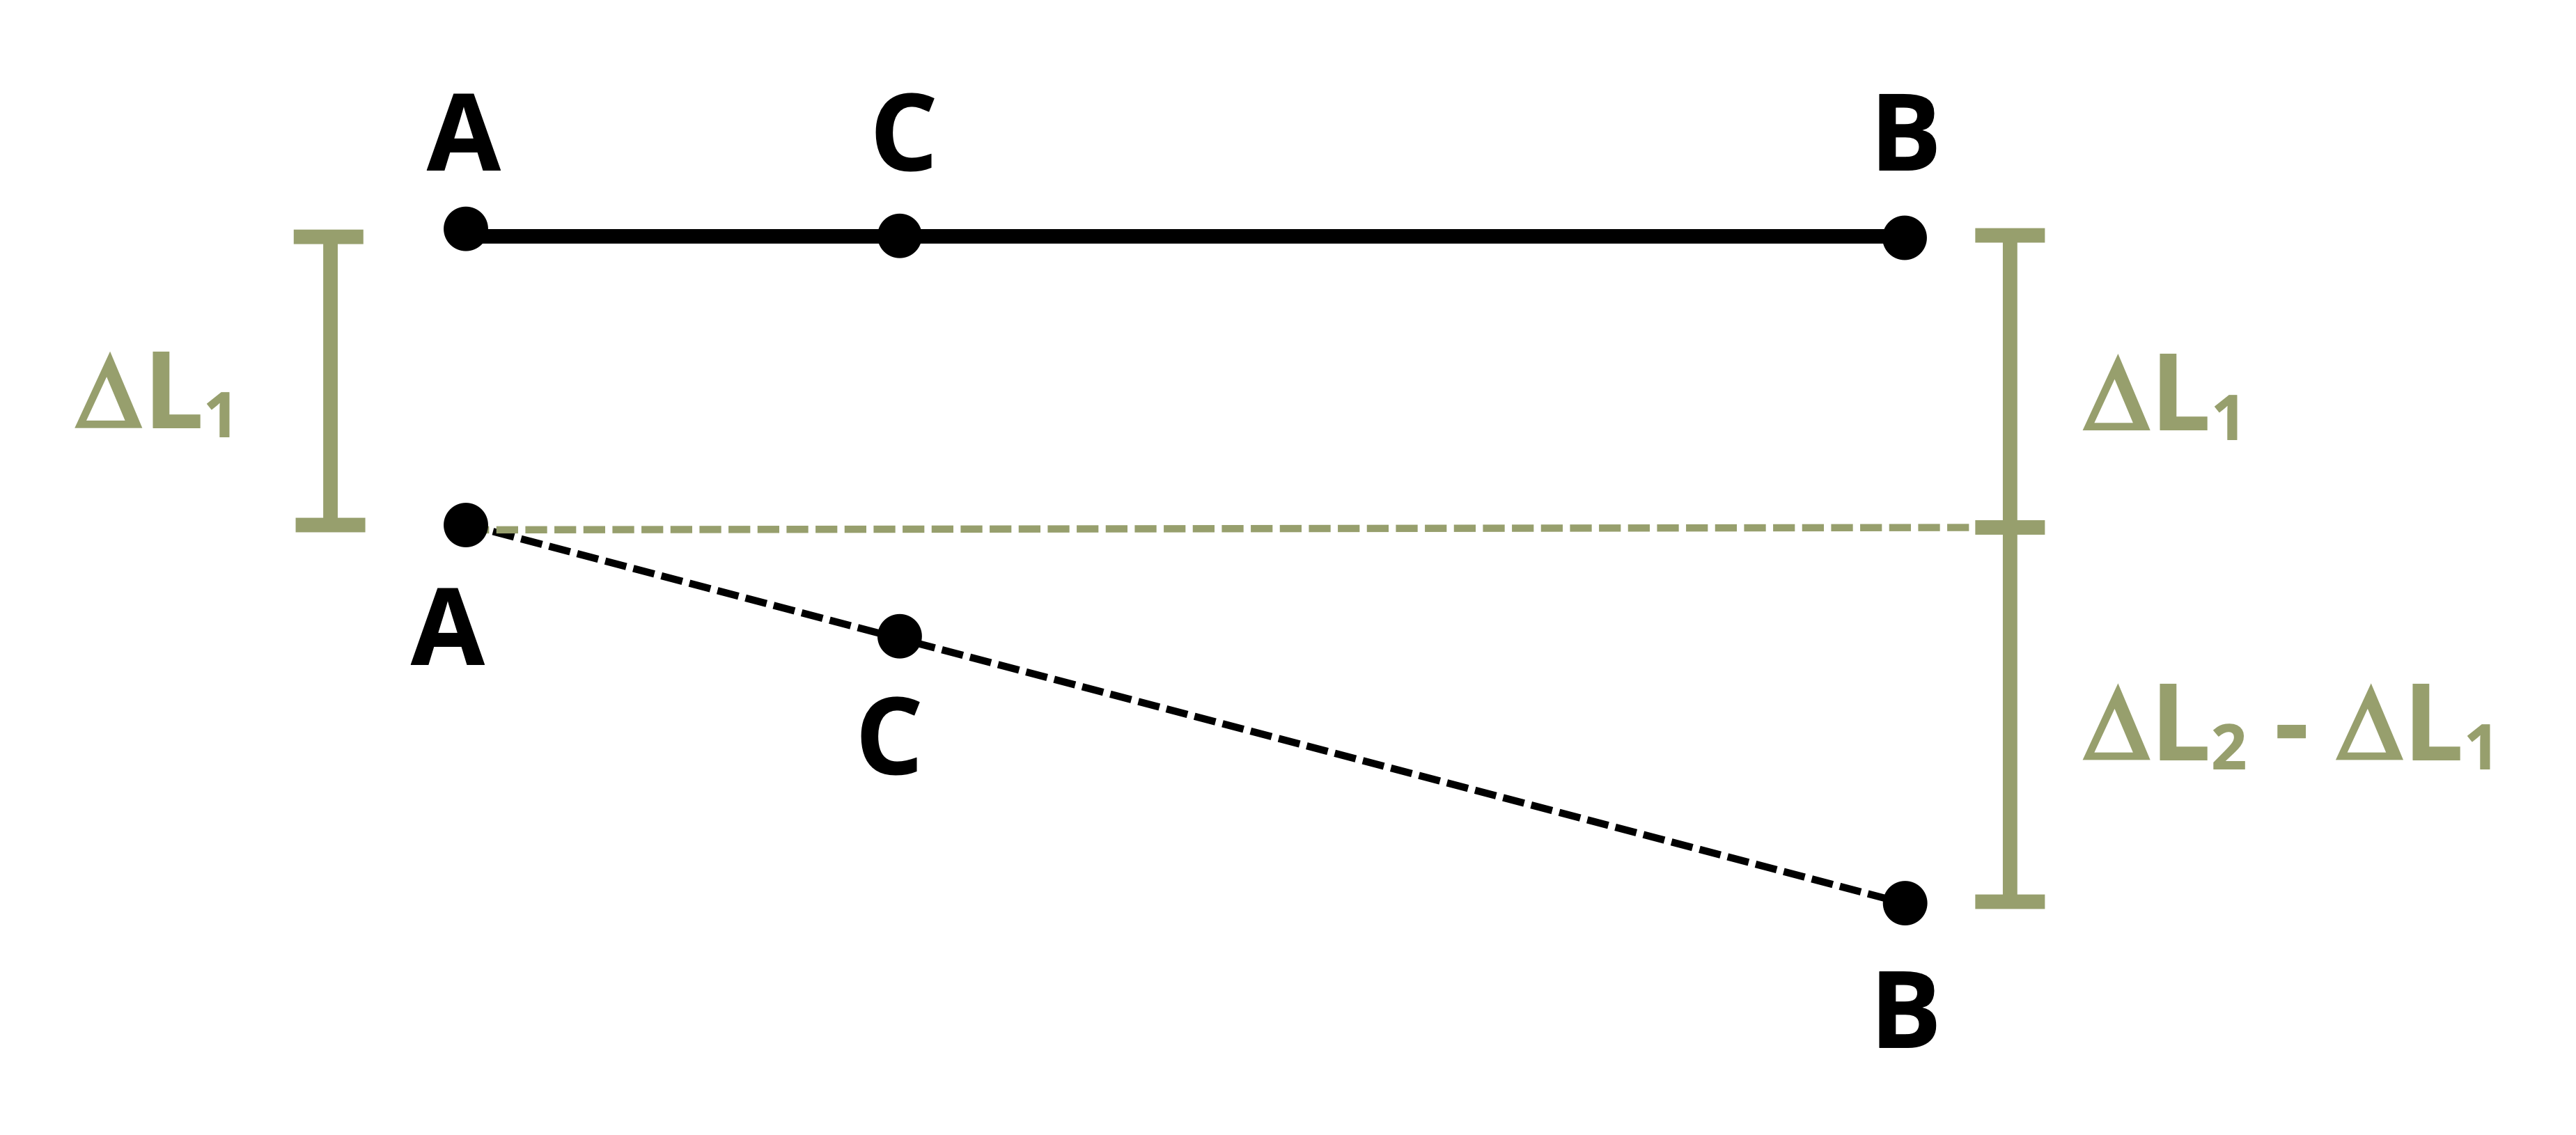
\includegraphics[width=3.94792in,height=\textheight]{images/PNGs/Figure 5.9.png}

}

\caption{Figure 5.8: Similar triangles for calculating deflection at a
point when both bars experience a change in length.}

\end{figure}%

\begin{tcolorbox}[enhanced jigsaw, colback=white, colframe=quarto-callout-note-color-frame, leftrule=.75mm, opacitybacktitle=0.6, colbacktitle=quarto-callout-note-color!10!white, arc=.35mm, bottomrule=.15mm, breakable, title={Example 5.4: Apply numbers to figure 5.6}, left=2mm, titlerule=0mm, toptitle=1mm, toprule=.15mm, opacityback=0, rightrule=.15mm, coltitle=black, bottomtitle=1mm]

A rigid beam is supported by two non-rigid poles and subjected to a
distributed load w = 75 kN/m. Pole 1 is made of steel (E = 200 GPa) and
has a diameter of 30 mm. Pole 2 is made of cast iron (E = 70 GPa) and
has a diameter of 50 mm. Determine the deflection at point C of the
rigid beam.

\begin{center}
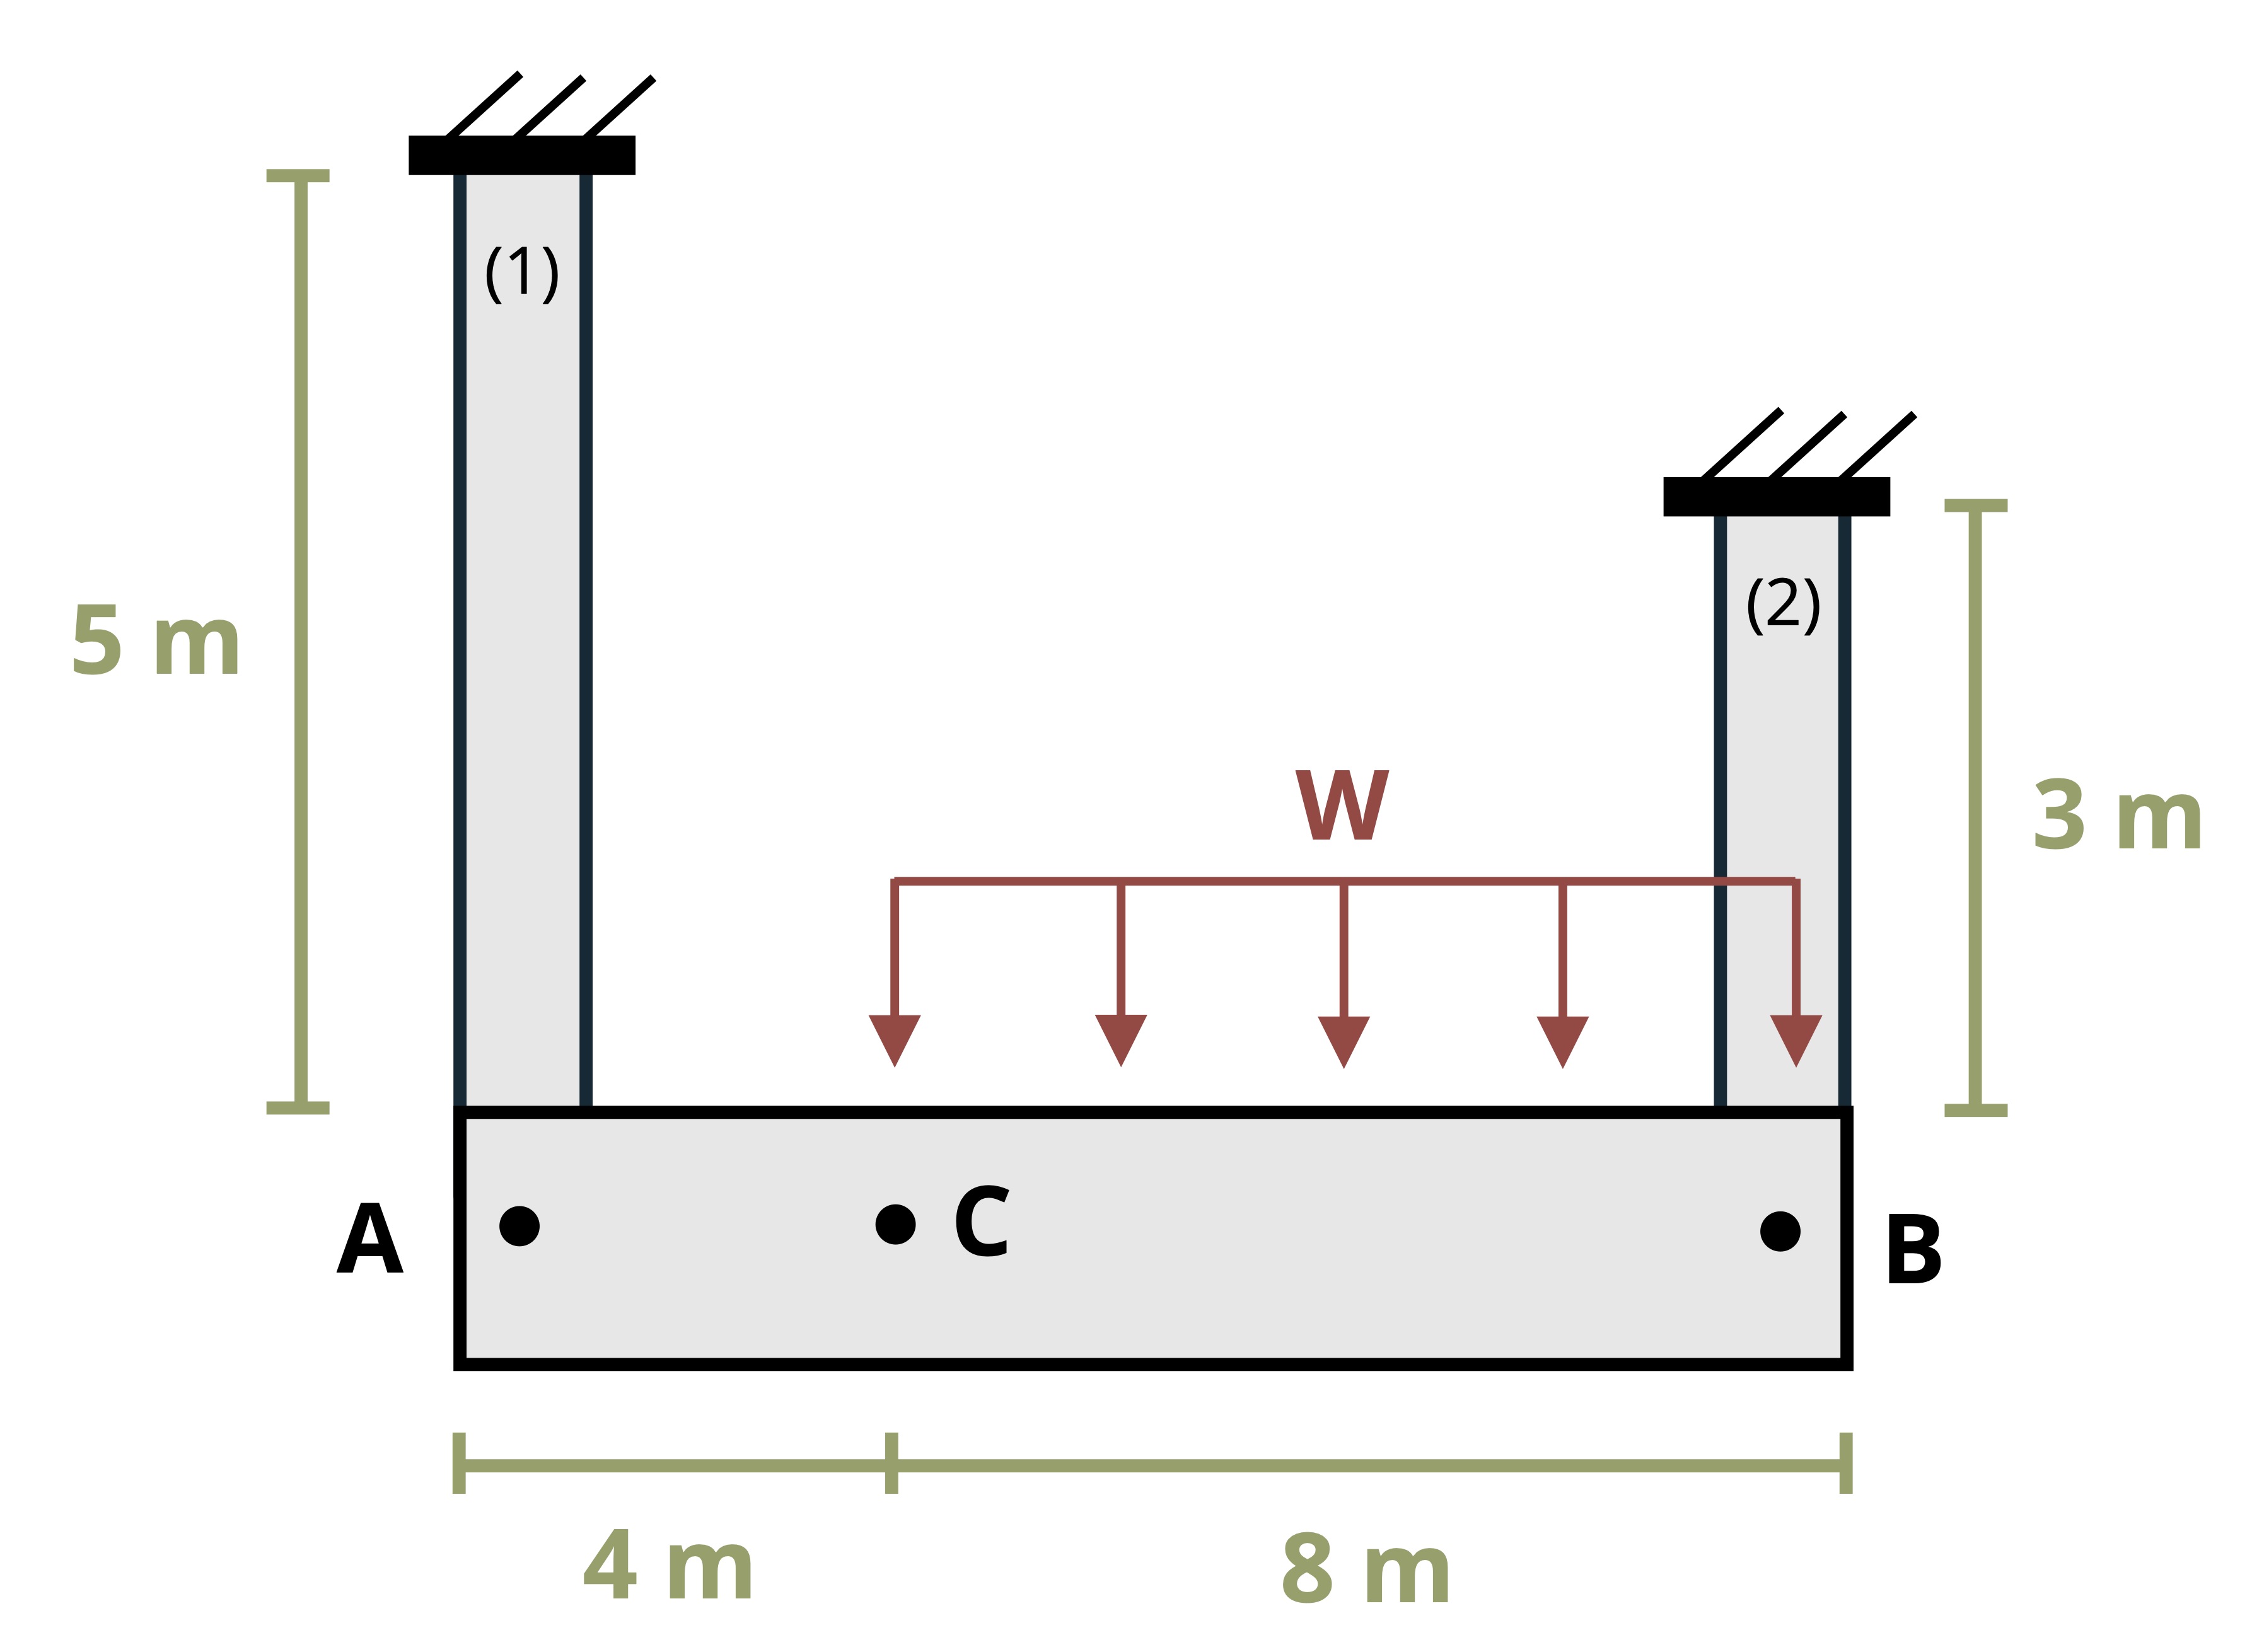
\includegraphics[width=3.19792in,height=\textheight]{images/PNGs/Example 5.4 part 1.png}
\end{center}

\begin{tcolorbox}[enhanced jigsaw, colback=white, colframe=quarto-callout-note-color-frame, leftrule=.75mm, opacitybacktitle=0.6, colbacktitle=quarto-callout-note-color!10!white, arc=.35mm, bottomrule=.15mm, breakable, title={Solution}, left=2mm, titlerule=0mm, toptitle=1mm, toprule=.15mm, opacityback=0, rightrule=.15mm, coltitle=black, bottomtitle=1mm]

Although the beam is rigid, poles 1 and 2 will both elongate. We can
find the force in each pole by drawing a free body diagram and applying
equilibrium equations.

\begin{center}
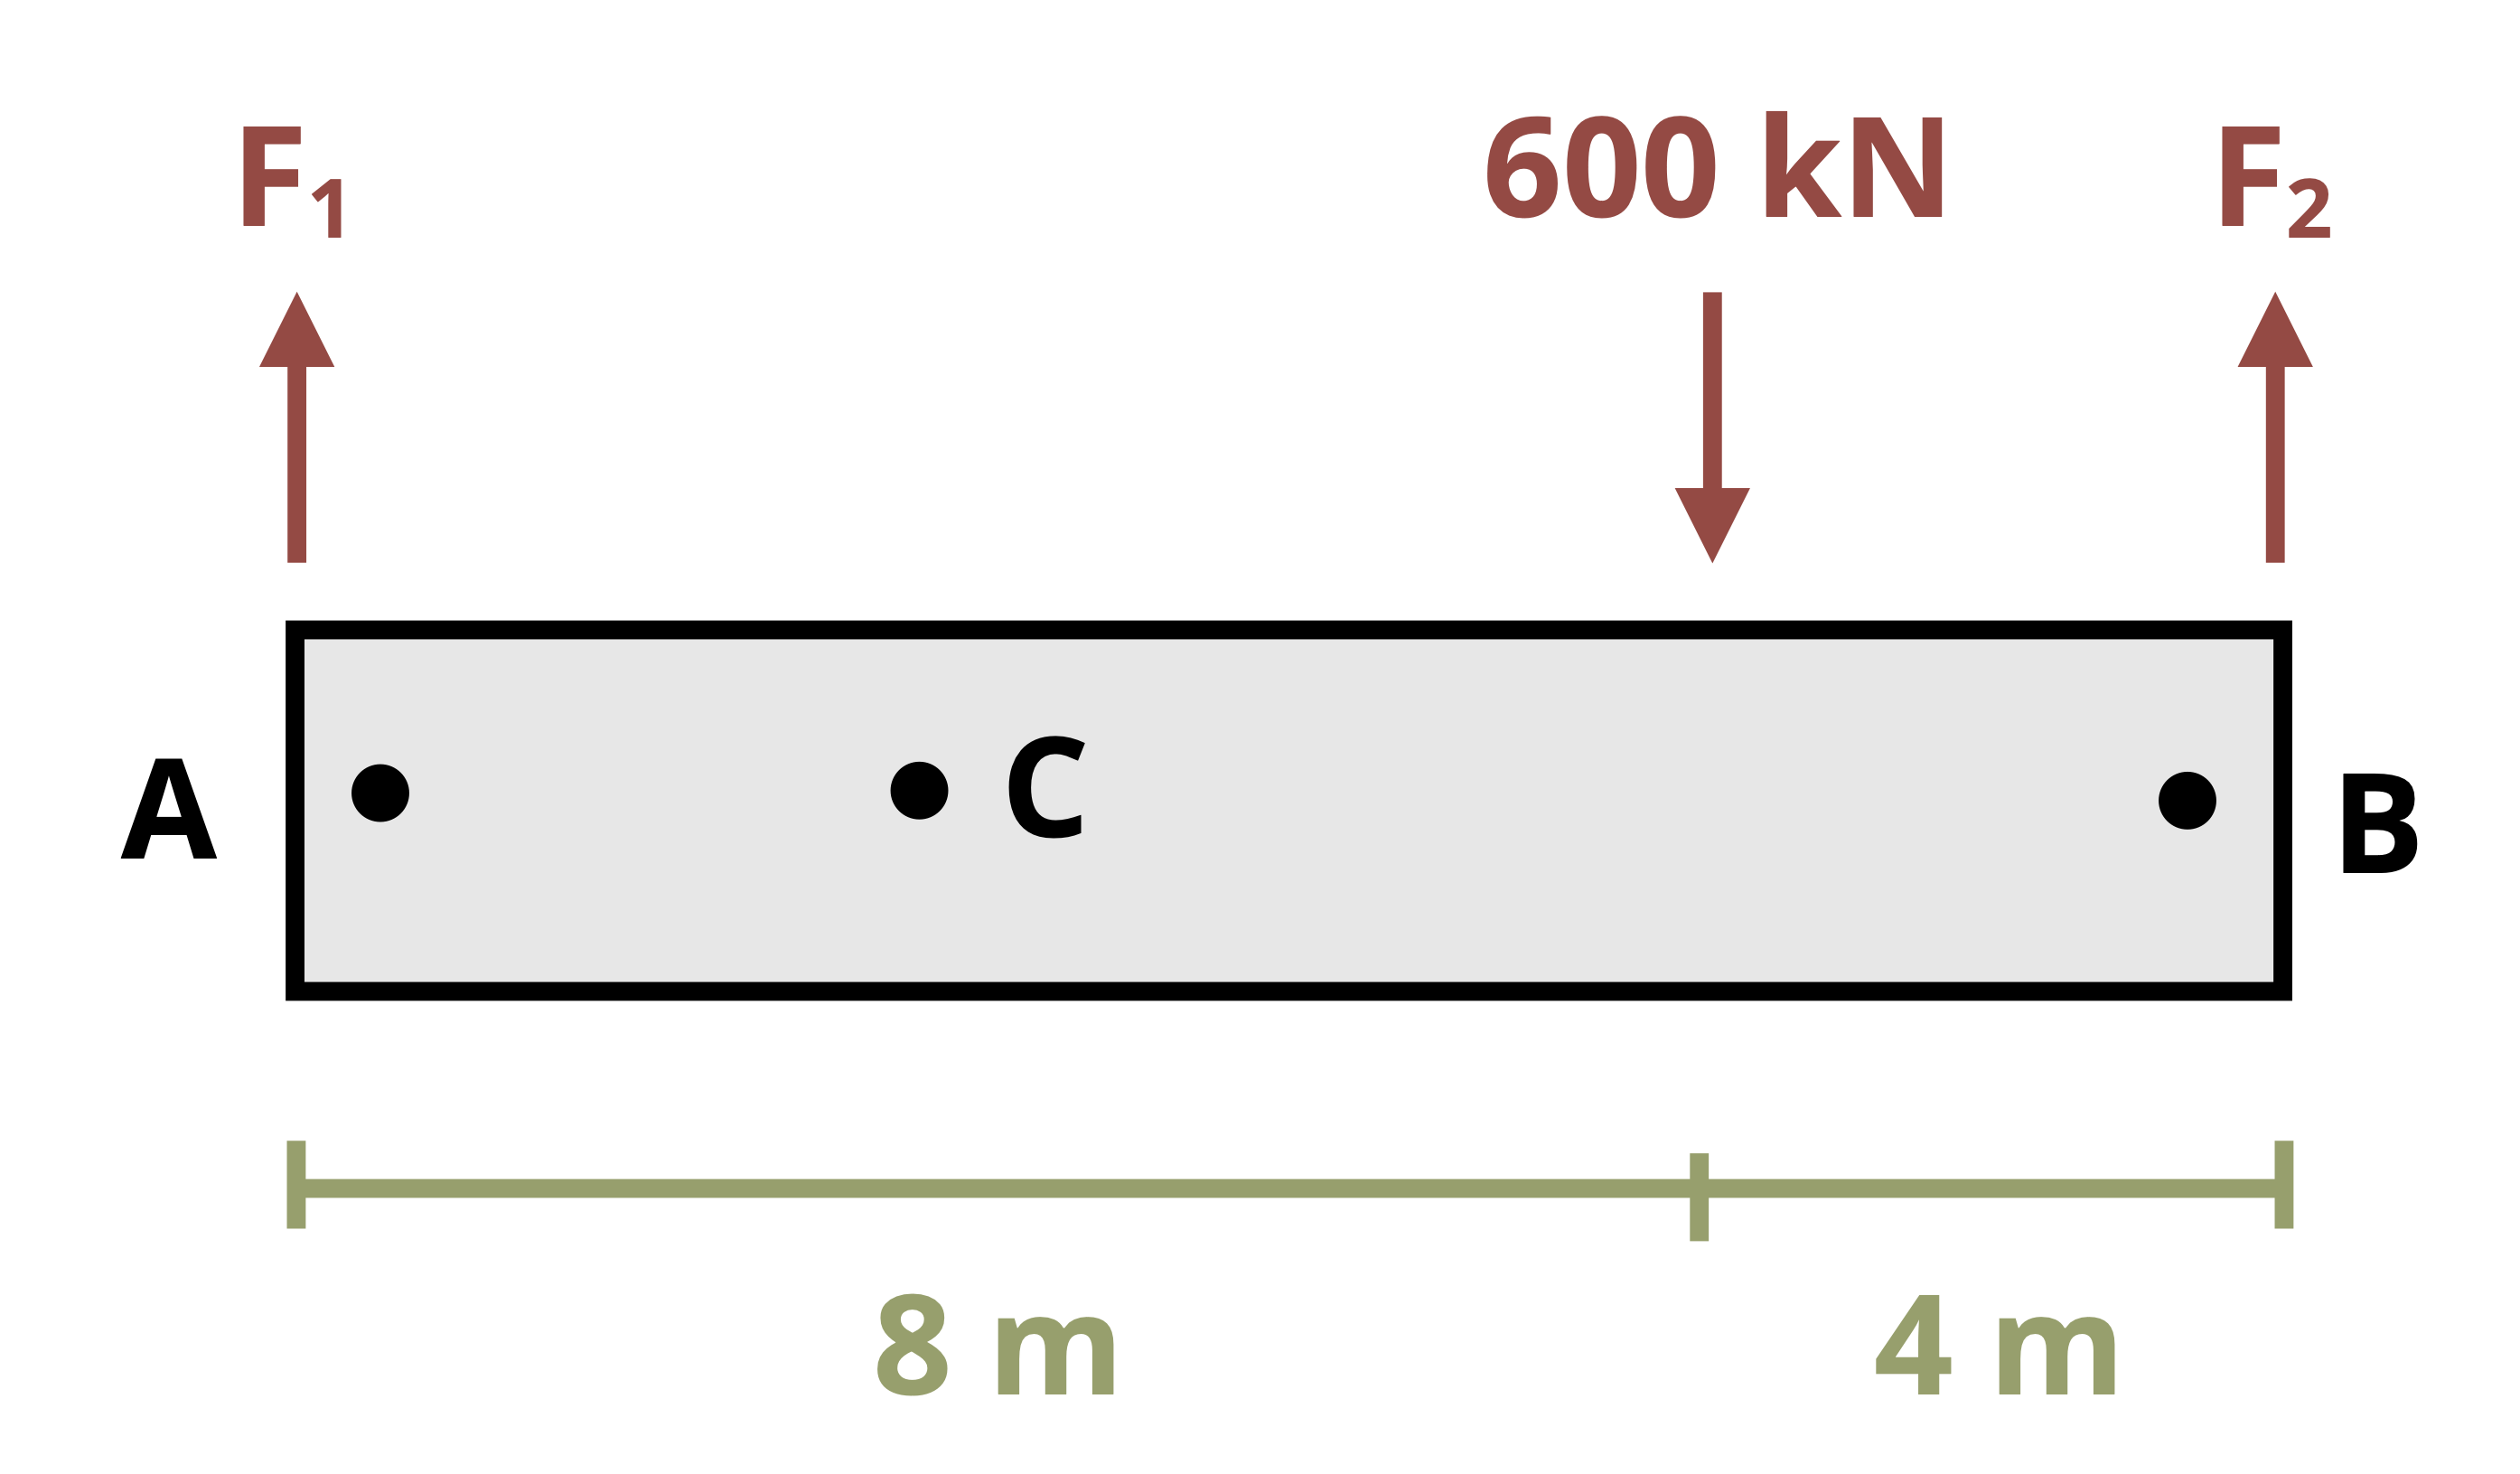
\includegraphics[width=2.55208in,height=\textheight]{images/PNGs/Example 5.4 part 2.png}
\end{center}

\[
\begin{gathered}
\sum M_A=0:-(600 * 8)+\left(F_2 * 12\right)=0 \rightarrow F_2=400 k N \\
\sum F_y=0: F_1-600+400=0 \rightarrow F_1=200 k N
\end{gathered}
\]

We can then calculate the change in length of each pole.

\[
\begin{aligned}
\Delta L_1 & =\frac{F_1 L_1}{A_1 E_1}=\frac{200000 * 5}{\pi * 0.015^2 * 200 * 10^9}=0.00707 \mathrm{~m}=7.07 \mathrm{~mm} \\
\Delta L_2 & =\frac{F_2 L_2}{A_2 E_2}=\frac{400000 * 3}{\pi * 0.025^2 * 70 * 10^9}=0.00873 \mathrm{~m}=8.73 \mathrm{~mm}
\end{aligned}
\]

To determine the deflection at point C, first determine that point B has
deflected (8.73 mm -- 7.07 mm) = 1.66 mm more than point A.

\begin{center}
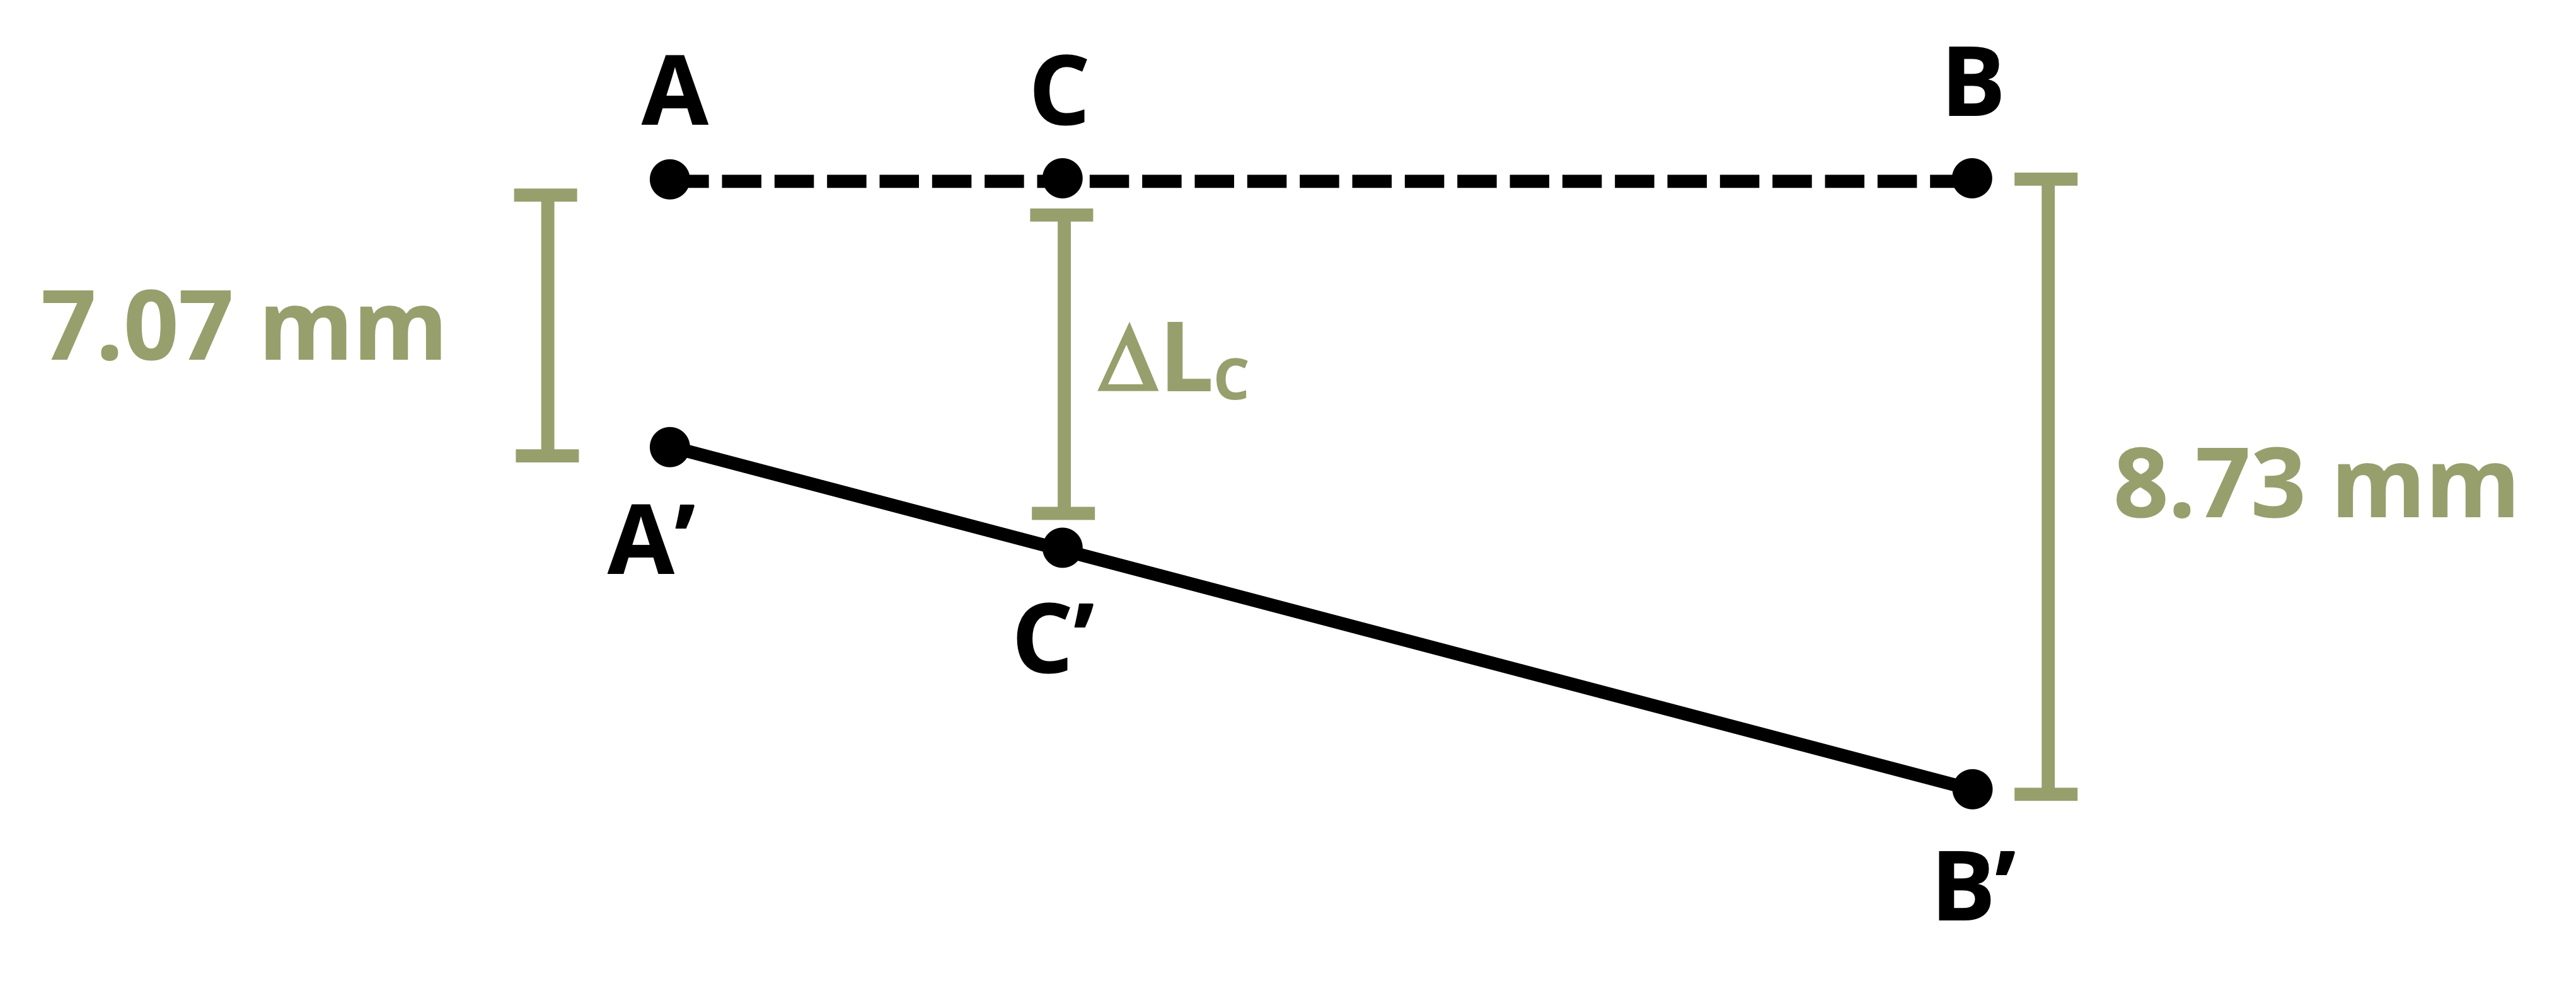
\includegraphics[width=3.23958in,height=\textheight]{images/PNGs/Example 5.4 part 3.png}
\end{center}

We can find how much more point C has deflected than point A by using
similar triangles.

\begin{center}
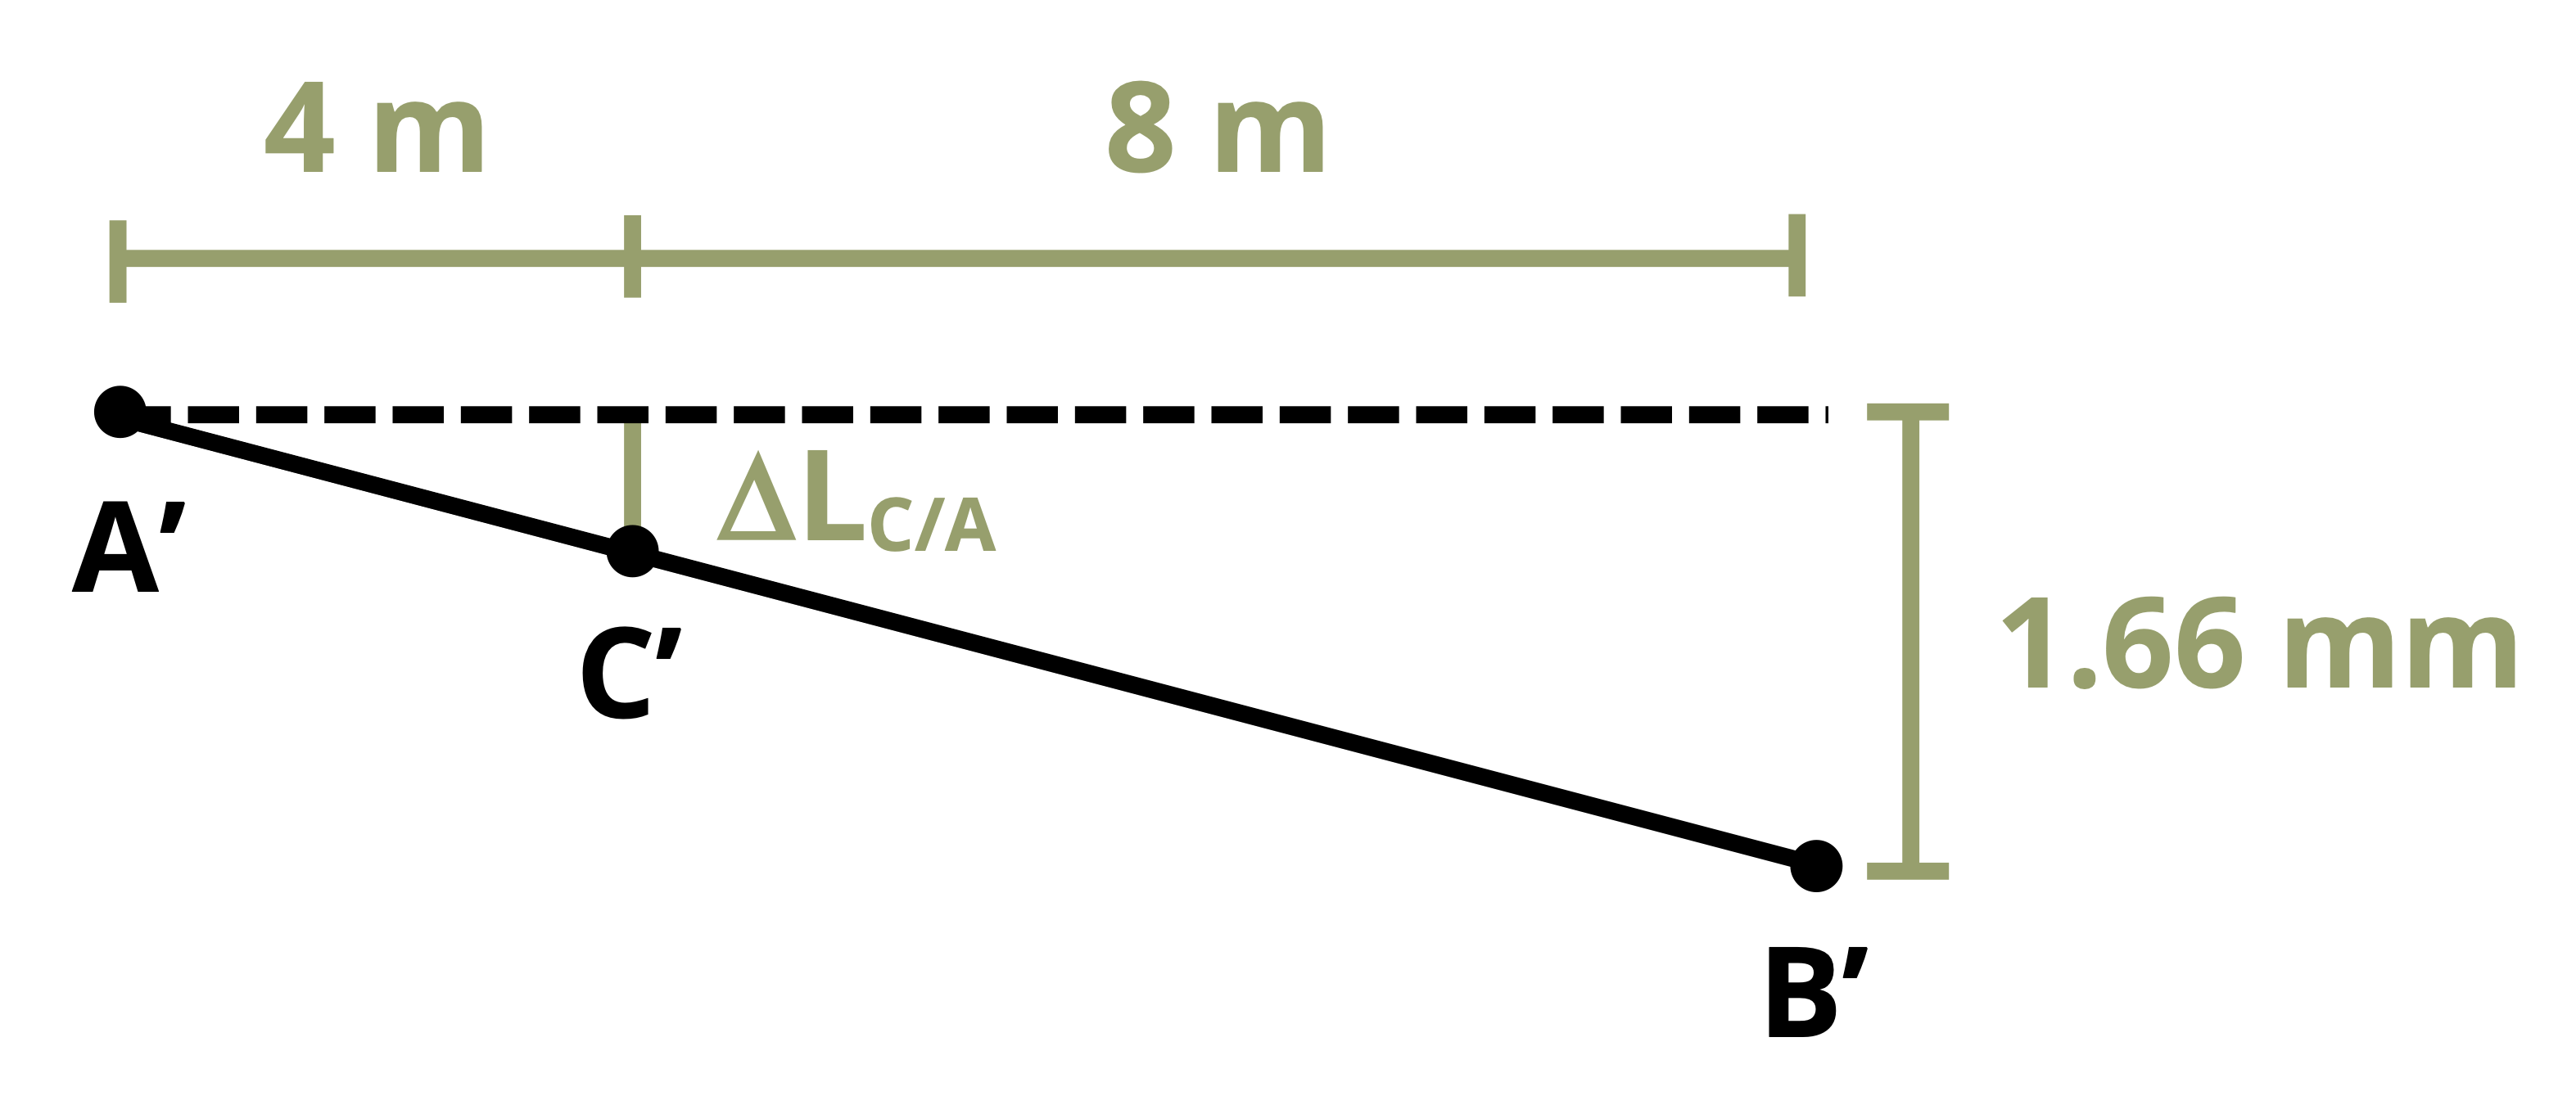
\includegraphics[width=2.63542in,height=\textheight]{images/PNGs/Example 5.4 part 4.png}
\end{center}

\[
\frac{1.66}{12}=\frac{\Delta L_{C / A}}{4} \rightarrow \Delta L_{C / A}=0.553 \mathrm{~mm}
\]

So point C deflects 0.553 mm more than point A, which is a total
deflection at point C of

\[
\Delta L_C=7.07 \mathrm{~mm}+0.553 \mathrm{~mm}=7.62 \mathrm{~mm}
\]

\end{tcolorbox}

\end{tcolorbox}

\begin{tcolorbox}[enhanced jigsaw, colback=white, colframe=quarto-callout-note-color-frame, leftrule=.75mm, opacitybacktitle=0.6, colbacktitle=quarto-callout-note-color!10!white, arc=.35mm, bottomrule=.15mm, breakable, title={Step-by-step: Deformation in series of bars}, left=2mm, titlerule=0mm, toptitle=1mm, toprule=.15mm, opacityback=0, rightrule=.15mm, coltitle=black, bottomtitle=1mm]

\begin{enumerate}
\def\labelenumi{\arabic{enumi}.}
\tightlist
\item
  Use equilibrium to determine the internal force in each bar.
\item
  Calculate the change in length of each bar using
  \(\Delta L=\frac{F L}{A E}\).
\item
  Use similar triangles to find the deflection at any point between the
  parallel bars.
\end{enumerate}

\end{tcolorbox}

\section{Statically Indeterminate
Problems}\label{statically-indeterminate-problems}

Click to expand

A statically indeterminate problem is one which has more unknowns than
we have equilibrium equations to solve for those unknowns. This is an
issue because it prevents us from finding the internal loads and we
therefore can't calculate stress or deformation.

We'll study two types of statically indeterminate problems. In the first
type there will be additional supports beyond those needed to maintain
equilibrium. These are known as redundant supports and they are quite
common in practice (Figure 5.9).

\begin{figure}[H]

{\centering 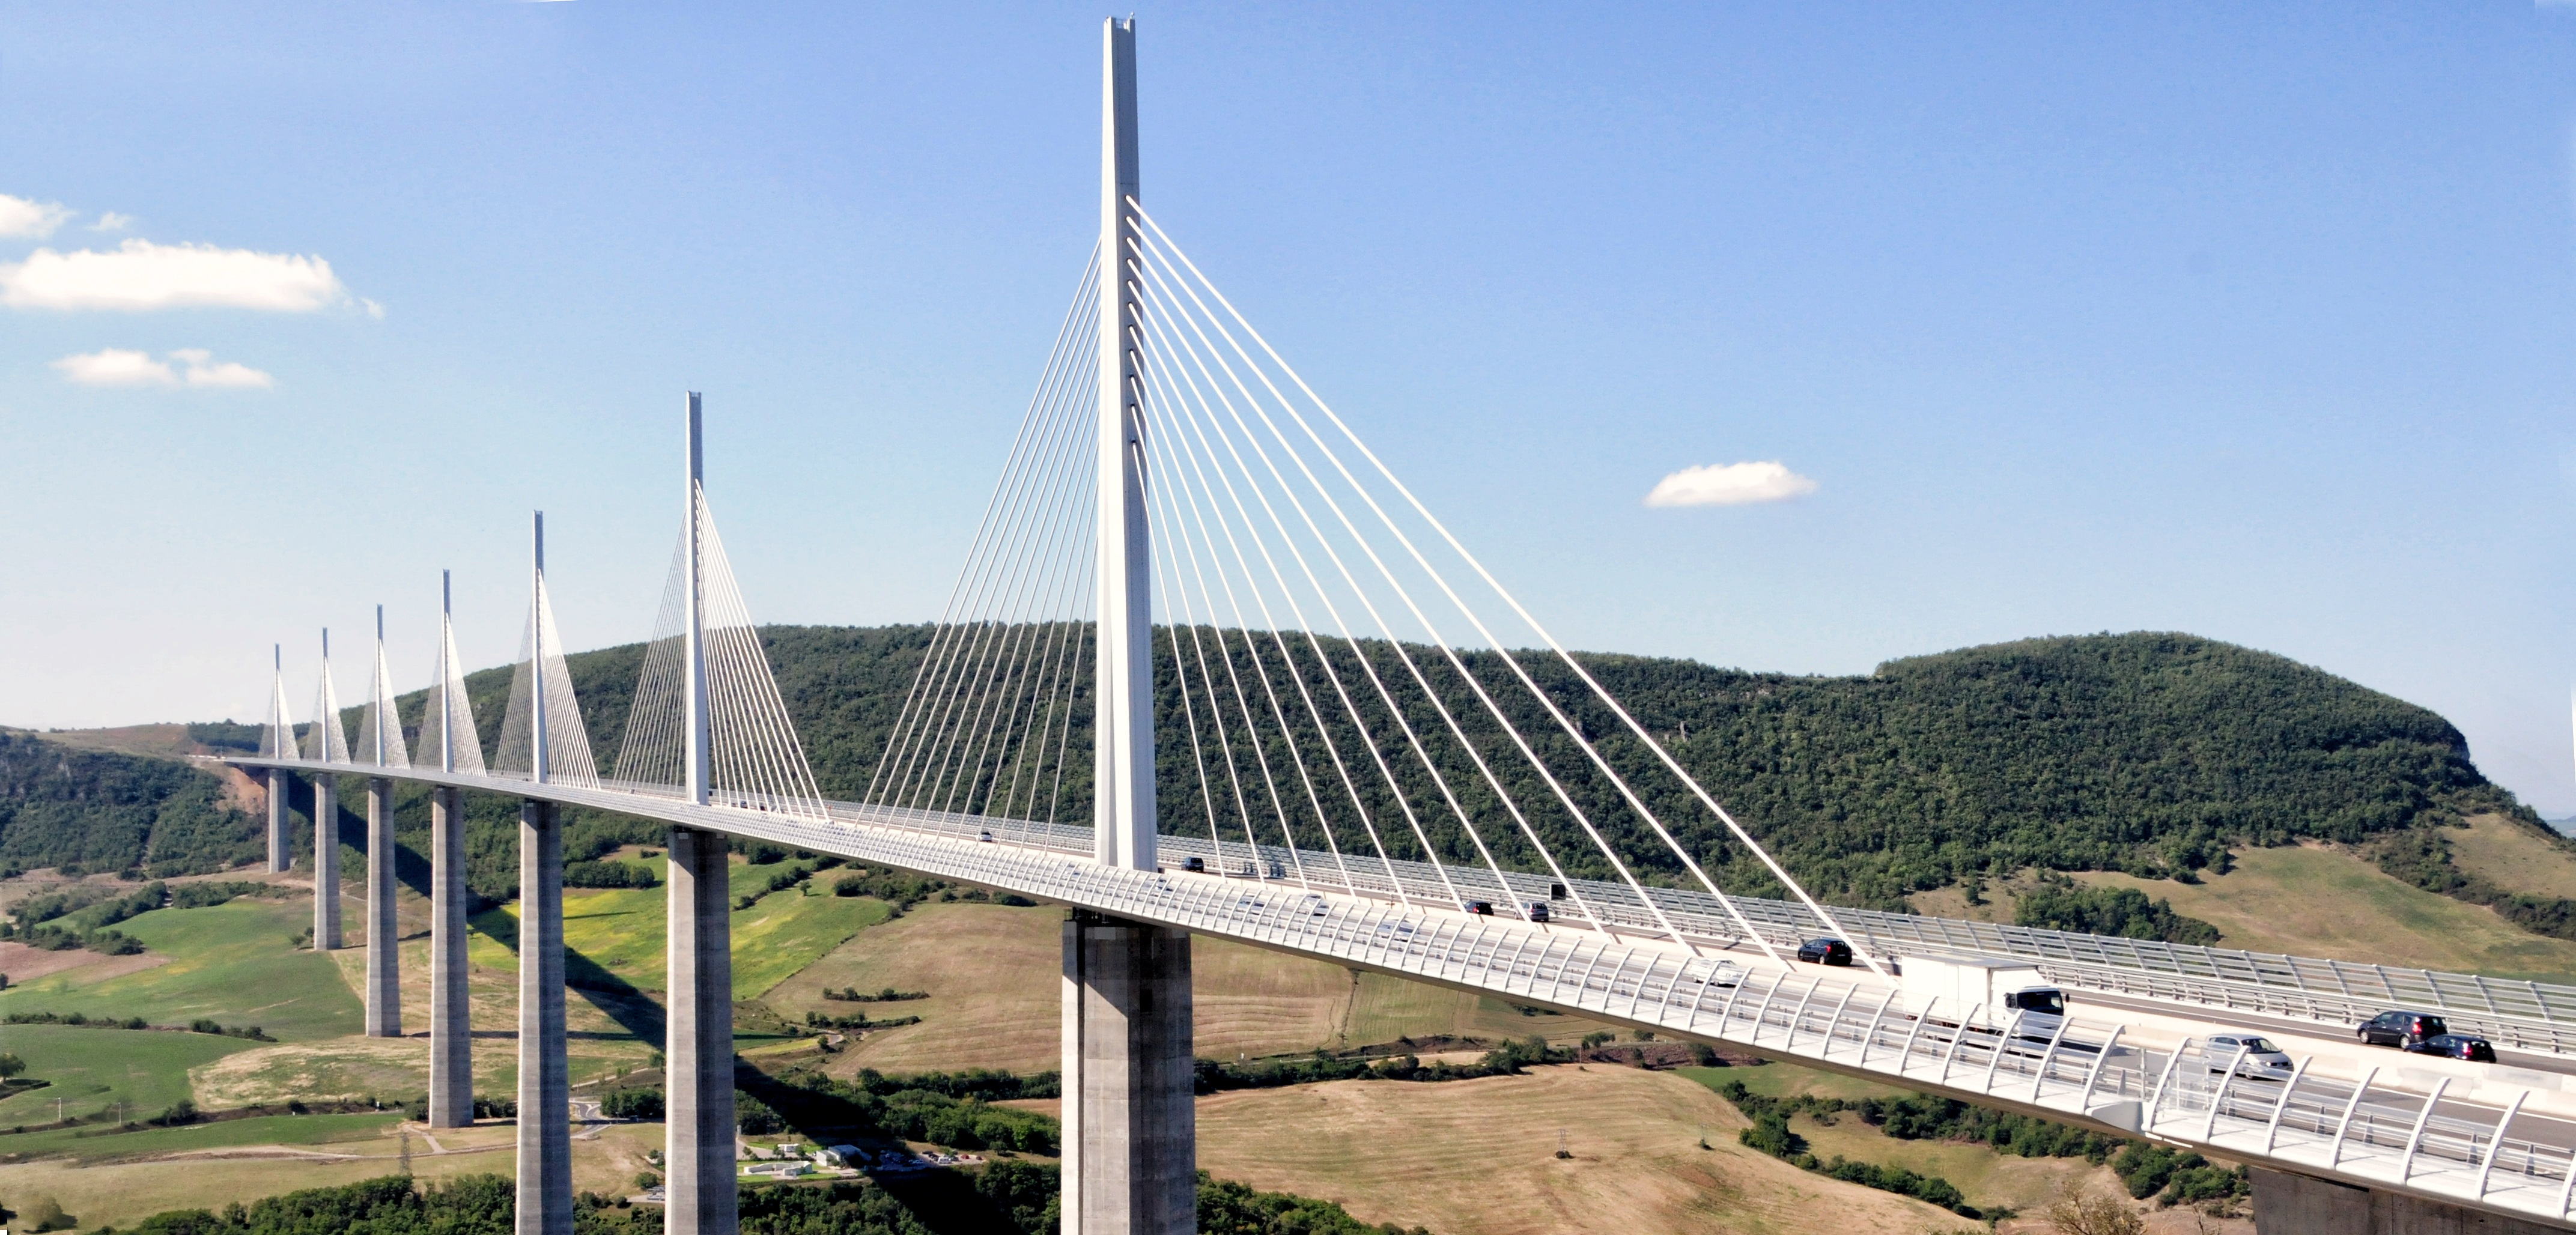
\includegraphics{images/PNGs/architecture-bridge-suspension-bridge-france-pillar-landmark-759379-pxhere.com.jpg}

}

\caption{Figure 5.9: An example of redundancy on a suspension bridge.
There are multiple supports and multiple cables at each support, such
that if one cable fails the entire structure does not collapse.}

\end{figure}%

In such problems, it is not possible to determine all of the reaction
forces using equilibrium alone. However, we can use our knowledge of
deformation to help. If a member is held between two supports then its
total deformation must be zero. Since the change in length depends on
the internal force in the member, this introduces an additional equation
to use alongside the equilibrium equations. There are two possible
approaches here.

\textbf{Approach 1}: To determine the reaction force at the redundant
support, begin by removing the redundant support from the problem and
determining the deformation that would occur if the support was not
there. Then replace the reaction force at the support, which will cause
the member to deform in the opposite direction (Figure 5.10).

\begin{figure}[H]

{\centering \includegraphics[width=5.40625in,height=\textheight]{images/PNGs/Figure 5.11.png}

}

\caption{Figure 5.10: (a) A bar held between two rigid supports. (b) A
free body diagram of the beam reveals that there are two unknowns but
only one equilibrium equation. (c) Removing one of the supports allows
the bar to elongate. (d) Replacing the support force causes the bar to
contract.}

\end{figure}%

The sum of these two deformations must equal the actual deformation of
the member. If the member is held between two rigid supports, the total
deformation will be zero. If there is a small gap or the supports allow
a certain amount of movement, the total deformation will be equal to the
size of this gap. Example 5.5 shows this process applied to a bar made
of 2 materials.

\begin{tcolorbox}[enhanced jigsaw, colback=white, colframe=quarto-callout-note-color-frame, leftrule=.75mm, opacitybacktitle=0.6, colbacktitle=quarto-callout-note-color!10!white, arc=.35mm, bottomrule=.15mm, breakable, title={Example 5.5: Bar between 2 supports, 2 materials, and areas}, left=2mm, titlerule=0mm, toptitle=1mm, toprule=.15mm, opacityback=0, rightrule=.15mm, coltitle=black, bottomtitle=1mm]

A 15-foot-tall concrete (E = 4,000 ksi) column has a square
cross-section of 6 in. by 6 in. A 10-foot-tall-copper (E = 17,000 ksi)
cylinder with an outer diameter of 4 in. and in inner diameter of 3 in.
is attached to the top of the concrete. The structure is fixed between
two supports. A force of 25 kips is applied as shown. Determine the
average normal stress in each material.

\begin{center}
\includegraphics[width=1.89583in,height=\textheight]{images/PNGs/Example 5.5 part 1.png}
\end{center}

\begin{tcolorbox}[enhanced jigsaw, colback=white, colframe=quarto-callout-note-color-frame, leftrule=.75mm, opacitybacktitle=0.6, colbacktitle=quarto-callout-note-color!10!white, arc=.35mm, bottomrule=.15mm, breakable, title={Solution}, left=2mm, titlerule=0mm, toptitle=1mm, toprule=.15mm, opacityback=0, rightrule=.15mm, coltitle=black, bottomtitle=1mm]

To determine the internal force in each material, we first need to find
the reaction forces at the supports. We would usually draw a free body
diagram and apply equilibrium equations to find these forces. However,
this won't work here because the problem is statically indeterminate.

\begin{center}
\includegraphics[width=1.15625in,height=\textheight]{images/PNGs/Example 5.5 part 2.png}
\end{center}

\[
\begin{aligned}
&\sum F_y=0: F_1+F_2-25=0\\
&F_1+F_2=25 \text { kips }
\end{aligned}
\]

To solve the statically indeterminate problem, remove one of the
supports and allow the structure to deform. Either support may be
removed. Let's remove the top support. In this scenario there is no load
in the copper cylinder and there is a compressive load of 25 kips in the
concrete column.

\begin{center}
\includegraphics[width=2.1875in,height=\textheight]{images/PNGs/Example 5.5 part 3.png}
\end{center}

The total deformation of the structure in this scenario is:

\[
\Delta L=\sum \frac{F L}{A E}=0-\frac{(25) *(15 * 12)}{(6 * 6) *(4,000)}=-0.03125 \mathrm{in}
\]

Then replace force F\textsubscript{1} and calculate the deformation
caused by this force. Since the force is applied at the top of the
structure, both the concrete and the copper will elongate.

\begin{center}
\includegraphics[width=2.1875in,height=\textheight]{images/PNGs/Example 5.5 part 4.png}
\end{center}

\[
\Delta L=\sum \frac{F L}{A E}=\frac{F_1 *(10 * 12)}{\pi\left(2^2-1.5^2\right) *(17,000)}+\frac{\left(F_1\right) *(15 * 12)}{(6 * 6) *(4,000)}=0.001284 F_1+0.00125 F_1=0.002534 F_1
\]

Since the structure is fixed at both ends, the actual total deformation
must be zero.

\[
-0.03125+0.002534 F_1=0 \rightarrow F_1=12.3 \mathrm{kips}
\]

Returning to our equilibrium equation, we can also find force
F\textsubscript{2}.

\[
F_1+F_2=25 \text { kips } \rightarrow 12.3+F_2=25 \rightarrow F_2=12.7 \text { kips }
\]

The internal force in the copper cylinder will be 12.3 kips and the
internal force in the concrete column will be 12.7 kips. Finally,
calculate the stress in each material. Note from our original free body
diagram that the copper cylinder is in tension while the concrete column
is in compression. We'll introduce a negative sign here to indicate
compressive stress in the concrete.

\[
\begin{aligned}
& \sigma_{\text {copper }}=\frac{N_1}{A_1}=\frac{12.3}{\pi\left(2^2-1.5^2\right)}=2.24 \mathrm{ksi} \\
& \sigma_{\text {concrete }}=-\frac{N_2}{A_2}=-\frac{12.7}{(6 * 6)}=-0.353 \mathrm{ksi}
\end{aligned}
\]

\end{tcolorbox}

\end{tcolorbox}

\textbf{Approach 2}: An alternate approach is to start by noting that
the total deformation of the bar must be zero. In the case shown in
Figure 5.11, we can say that the deformation of segment 1 plus the
deformation of segment 2 must add up to zero.

\begin{figure}[H]

{\centering \includegraphics{images/PNGs/Figure 5.12.png}

}

\caption{Figure 5.11: (a) A bar held between two rigid supports. (b) A
free body diagram of the bar.}

\end{figure}%

The internal load in segment 1 is FA and the internal load in segment 2
is FB, so there are currently two unknowns. We may use an equilibrium
equation to solve for these two unknowns simultaneously.

\[
\begin{aligned} & \frac{F_A L_1}{A_1 E_1}+\frac{F_B L_2}{A_2 E_2}=0 \\ & F-F_A-F_B=0\end{aligned}\]

Example 5.6 re-solves Example 5.5 using this method instead.

\begin{tcolorbox}[enhanced jigsaw, colback=white, colframe=quarto-callout-note-color-frame, leftrule=.75mm, opacitybacktitle=0.6, colbacktitle=quarto-callout-note-color!10!white, arc=.35mm, bottomrule=.15mm, breakable, title={Example 5.6: Bar between 2 supports, 2 materials, and areas}, left=2mm, titlerule=0mm, toptitle=1mm, toprule=.15mm, opacityback=0, rightrule=.15mm, coltitle=black, bottomtitle=1mm]

A 15-foot-tall concrete (E = 4,000 ksi) column has a square
cross-section of 6 in. by 6 in. A 10-foot-tall-copper (E = 17,000 ksi)
cylinder with an outer diameter of 4 in. and in inner diameter of 3 in.
is attached to the top of the concrete. The structure is fixed between
two supports. A force of 25 kips is applied as shown. Determine the
average normal stress in each material.

\begin{center}
\includegraphics[width=1.94792in,height=\textheight]{images/PNGs/Example 5.6 part 1.png}
\end{center}

\begin{tcolorbox}[enhanced jigsaw, colback=white, colframe=quarto-callout-note-color-frame, leftrule=.75mm, opacitybacktitle=0.6, colbacktitle=quarto-callout-note-color!10!white, arc=.35mm, bottomrule=.15mm, breakable, title={Solution}, left=2mm, titlerule=0mm, toptitle=1mm, toprule=.15mm, opacityback=0, rightrule=.15mm, coltitle=black, bottomtitle=1mm]

As before, begin with an equilibrium equation that relates the support
loads to the applied load. In this equation we use the convention that
forces pointing upwards are positive and forces pointing downwards are
negative.

\begin{center}
\includegraphics[width=1.26042in,height=\textheight]{images/PNGs/Example 5.6 part 2.png}
\end{center}

\[
\begin{aligned}
& \sum F_y=0: F_1+F_2-25=0 \\
& F_1+F_2=25 \mathrm{kips}
\end{aligned}
\]

This bar consists of 2 segments -- the copper cylinder (segment 1) and
the concrete column (segment 2). Since the bar is held between two rigid
supports, the total deformation of these two segments must sum to zero.
Note that in this diagram segment 1 is in tension while segment 2 is in
compression. We must be consistent with the sign convention that tension
is positive and compression is negative.

\[
\frac{F_1 L_1}{A_1 E_1}-\frac{F_2 L_2}{A_2 E_2}=0
\]

Here F1 and F2 are the internal forces in segments 1 and 2 of the bar.
These will be the same as the reaction loads at the supports that we are
trying to solve for.

\[
\frac{F_1 *(10 * 12)}{\pi\left(2^2-1.5^2\right) *(17,000)}-\frac{F_2 *(15 * 12)}{(6 * 6) *(4,000)}=0
\]

Rearrange the equilibrium equation and substitute into the deformation
equation.

\[
\begin{gathered}
F_1=25-F_2 \\
\frac{\left(25-F_2\right) *(10 * 12)}{\pi\left(2^2-1.5^2\right) *(17,000)}-\frac{F_2 *(15 * 12)}{(6 * 6) *(4,000)}=0
\end{gathered}
\]

Then simplify and solve for force F2.

\[
\begin{gathered}
0.0321-0.001284 F_2-0.00125 F_2=0 \\
0.0321=0.002534 F_2 \\
F_2=12.7 \mathrm{kips}
\end{gathered}
\]

Then use the equilibrium equation again to find F1.

\[
F_1=25-12.7=12.3 \mathrm{kips}
\]

These are the same reactions that we found in Example 5.5 when we solved
this problem using the other approach. From here we can find the stress
in each material as before, noting again from our diagram that segment 2
is in compression.

\[
\begin{aligned}
& \sigma_{\text {copper }}=\frac{N_1}{A_1}=\frac{12.3}{\pi\left(2^2-1.5^2\right)}=2.24 \mathrm{ksi} \\
& \sigma_{\text {concrete }}=-\frac{N_2}{A_2}=-\frac{12.7}{(6 * 6)}=-0.353 \mathrm{ksi}
\end{aligned}
\]

\end{tcolorbox}

\end{tcolorbox}

The second type of indeterminate problem involves two materials bonded
together in parallel. In these problems it's possible to find the
reactions at the supports, but not possible to find the internal force
in each material using only equilibrium (Figure 5.12).

\begin{figure}[H]

{\centering \includegraphics[width=2.94792in,height=\textheight]{images/PNGs/Figure 5.13.png}

}

\caption{Figure 5.12: When two materials in parallel are subjected to
force F, the force is split between the two materials
(F\textsubscript{1} and F\textsubscript{2}). By equilibrium
F\textsubscript{1} + F\textsubscript{2} = F but this is not sufficient
to find the force in each material.}

\end{figure}%

We have one equilibrium equation but two unknown internal forces.
However, since the materials are bonded together we can say that they
must deform by the same amount. By setting the deformation for each
material equal to each other we can define a second equation that
involves the two internal forces and, combined with the equilibrium
equation, we can now solve for both internal forces. See Example 5.7 for
a demonstration.

\begin{tcolorbox}[enhanced jigsaw, colback=white, colframe=quarto-callout-note-color-frame, leftrule=.75mm, opacitybacktitle=0.6, colbacktitle=quarto-callout-note-color!10!white, arc=.35mm, bottomrule=.15mm, breakable, title={Example 5.7: 2 materials in parallel}, left=2mm, titlerule=0mm, toptitle=1mm, toprule=.15mm, opacityback=0, rightrule=.15mm, coltitle=black, bottomtitle=1mm]

A 20-ft-tall concrete (E = 4,000 ksi) column has a square cross-section
6 inches on each side. It is reinforced by six pieces of steel (E =
30,000 ksi) rebar that extend through the length of the column. Each has
a diameter of 0.5 inches. The column is subjected to a compressive load
of 70 kips. Determine the stress in each material.

\begin{center}
\includegraphics[width=1.84375in,height=\textheight]{images/PNGs/Example 5.7 part 1.png}
\end{center}

\begin{tcolorbox}[enhanced jigsaw, colback=white, colframe=quarto-callout-note-color-frame, leftrule=.75mm, opacitybacktitle=0.6, colbacktitle=quarto-callout-note-color!10!white, arc=.35mm, bottomrule=.15mm, breakable, title={Solution}, left=2mm, titlerule=0mm, toptitle=1mm, toprule=.15mm, opacityback=0, rightrule=.15mm, coltitle=black, bottomtitle=1mm]

The 70 kips force will be split between the two materials. We need to
find the force in each material before we can calculate the stress.
Start by cutting a cross-section through the column, drawing a free body
diagram, and writing an equilibrium equation.

\begin{center}
\includegraphics[width=1.42708in,height=\textheight]{images/PNGs/Example 5.7 copy.png}
\end{center}

\[
\sum F_y=0: F_C+F_S=70 \mathrm{kips}
\]

This problem is statically indeterminate, since we have two unknowns and
only one equilibrium equation. However, since the two materials are
bonded together we can say that they must both deform the same amount.

\[
\Delta L_C=\Delta L_S
\]

Since we know \(\Delta L=\frac{F L}{A E}\)

\[
\frac{F_C L_C}{A_C E_C}=\frac{F_S L_S}{A_S E_S}
\]

The length of both materials is 20 ft, so this term will cancel.

Although the steel is 6 individual pieces, it's fine to determine the
total area of the steel and the total force in the steel. The total area
of the steel is \(A_S=6 * \pi * 0.25^2=1.178 \mathrm{in}^2\)

For the area of the concrete, calculate the area of the square and then
remove the area of the 6 rebar rods.

\[
A_C=(6 * 6)-1.178=34.82 \mathrm{in.}^2
\]

Substitute these into the deformation equation and rearrange.

\[
\begin{gathered}
\frac{F_C}{34.82 * 4,000}=\frac{F_S}{1.178 * 30,000} \\
F_C=F_S\left[\frac{34.82 * 4,000}{1.178 * 30,000}\right] \\
F_C=3.941 F_S
\end{gathered}
\]

Substitute this into the equilibrium equation.

\[
\begin{gathered}
F_C+F_S=70 \mathrm{kips} \\
3.941 F_S+F_S=70 \mathrm{kips} \\
4.941 F_S=70 \mathrm{kips} \\
F_S=14.2 \mathrm{kips}
\end{gathered}
\]

Then since
\(F_C=3.941 F_S \rightarrow F_C=3.941 * 14.2=55.8 \mathrm{kips}\)

Now that we know the force in each material, we can calculate the stress
in each material.

\[
\begin{aligned}
& \sigma_S=\frac{14.2}{1.178}=12.0 \mathrm{ksi} \\
& \sigma_C=\frac{55.8}{34.82}=1.60 \mathrm{ksi}
\end{aligned}
\]

\end{tcolorbox}

\end{tcolorbox}

\begin{tcolorbox}[enhanced jigsaw, colback=white, colframe=quarto-callout-note-color-frame, leftrule=.75mm, opacitybacktitle=0.6, colbacktitle=quarto-callout-note-color!10!white, arc=.35mm, bottomrule=.15mm, breakable, title={Step-by-step: Statically indeterminate axial problems}, left=2mm, titlerule=0mm, toptitle=1mm, toprule=.15mm, opacityback=0, rightrule=.15mm, coltitle=black, bottomtitle=1mm]

\textbf{Problems with redundant supports}

Approach 1:

\begin{enumerate}
\def\labelenumi{\arabic{enumi}.}
\tightlist
\item
  Write out equilibrium equations. There will be too many unknowns, so
  put these to one side for now.
\item
  Remove one of the supports and calculate the amount of deformation
  that would occur if the support wasn't there using
  \(\Delta L_1=\sum \frac{F L}{A E}\)
\item
  Replace the force from the removed support and determine the
  deformation, \(\Delta L_2\), caused by this force in terms of the
  force itself.
\item
  Set \(\Delta L_1 + \Delta L_2\) equal to the total allowed deformation
  for the bar and use this to solve for the unknown force at the
  redundant support.
\item
  Now that one force is known, use the equilibrium equations to
  determine the other unknown forces.
\end{enumerate}

Approach 2:

\begin{enumerate}
\def\labelenumi{\arabic{enumi}.}
\tightlist
\item
  Draw a free body diagram of the entire structure and write out the
  relevant equilibrium equations. For axial loads this will just be one
  sum of force equation, either horizontally or vertically depending on
  the applied loading.
\item
  Write an equation saying that the total deformation in each segment of
  the bar must sum to the total deformation of the bar (zero if the bar
  is held between two rigid supports). A new segment must be made any
  time the internal load, cross-sectional area, or material changes.
\item
  This deformation equation will involve the same two unknowns as the
  equilibrium equation. Solve these equations simultaneously to find the
  reaction loads at the supports
\end{enumerate}

\textbf{Problems with two materials in parallel}

\begin{enumerate}
\def\labelenumi{\arabic{enumi}.}
\tightlist
\item
  Cut a cross-section through the member and set up an equilibrium
  equation for the internal forces where the internal forces will sum to
  equal the external applied force.
\item
  Set the deformation of the two materials equal.
\item
  Solve the deformation equation and equilibrium equation simultaneously
  to determine the internal force in each material.
\end{enumerate}

\end{tcolorbox}

\section{Thermal Deformation}\label{thermal-deformation}

Click to expand

So far, we've studied the effects of axial forces on an object and how
they create stresses and deformations. Temperature changes will also
cause an object to deform. The strain due to temperature can be
predicted by:

\[
\varepsilon_T=\alpha \Delta T\]

where

\emph{𝜀\textsubscript{T} = Thermal strain}

\emph{𝛼 = Coefficient of thermal expansion}
\(\left[\frac{1}{{ }^{\circ} C}, \frac{1}{{ }^{\circ} F}\right]\)

\emph{ΔT = Change in temperature}
\(\left[{ }^{\circ} \mathrm{C},{ }^{\circ} \mathrm{F}\right]\)

As before, strain is dimensionless. The coefficient of thermal expansion
is a material constant that can be looked up in handbooks or in Appendix
C. Note that for a given change in temperature, the thermal strain will
be the same in the axial and transverse directions.

Since strain is also defined as \(\varepsilon=\frac{\Delta L}{L}\), we
can also predict the deformation due to a change in temperature:

\[
\varepsilon_T=\alpha \Delta T=\frac{\Delta L}{L} \rightarrow \Delta L=\alpha \Delta T L\]

If the object is free to expand or contract this doesn't cause any
issues and is easy to account for. Many real applications will include a
small gap to allow for changes in length due to temperature changes
(Figure 5.13). It is even possible that an object is subjected to both a
physical force and a temperature change and the total change in length
is simply the sum of these effects:

\[
\Delta L=\Delta L_F+\Delta L_T=\frac{F L}{A E}+\alpha \Delta T L\]

\strut \\

\textbf{Figure 5.13} -- Expansion joint on a bridge, allowing for
thermal expansion and contraction of the bridge as temperature changes
through the year.

However if we do not design a gap, or if the gap is not large enough,
then the object is not free to expand or contract. As the member pushes
or pulls on its supports, a physical force is created. This in turn
creates a stress in the object and these stresses can be very large.
Such problems are statically indeterminate as the force applied on the
member by the support is unknown and can't be found using only
equilibrium. Solving these problems is very similar to solving the first
type of statically indeterminate problem. First, remove a support and
determine the amount of deformation that would occur due to the change
in temperature if the object were free to deform. Then replace the force
from the removed support, which will cause the object to deform in the
other direction. The sum of these two deformations will equal the total
deformation of the member as before. Example 5.8 works through an
indeterminate thermal expansion problem.

\begin{tcolorbox}[enhanced jigsaw, colback=white, colframe=quarto-callout-note-color-frame, leftrule=.75mm, opacitybacktitle=0.6, colbacktitle=quarto-callout-note-color!10!white, arc=.35mm, bottomrule=.15mm, breakable, title={Example 5.8: Indeterminate thermal expansion without gap. Then add gap
and rework}, left=2mm, titlerule=0mm, toptitle=1mm, toprule=.15mm, opacityback=0, rightrule=.15mm, coltitle=black, bottomtitle=1mm]

Steel (E = 200 GPa, α = 11.7x10-6 /°C) train rails are laid end-to-end.
Each rail is 20 meters long. A small section of this track is shown
below. The rails are laid in winter when the temperature is 0° C. In
summer, the maximum temperature is 40°C. Determine the compressive
stress in the rail as a result of the temperature change if:

(a) In a particular section of track, the rails are laid with no gap
between them.

(b) In another section, the rails have a 5-mm-gap between them.

\begin{center}
\includegraphics[width=4.33333in,height=\textheight]{images/PNGs/Example 5.8.png}
\end{center}

\begin{tcolorbox}[enhanced jigsaw, colback=white, colframe=quarto-callout-note-color-frame, leftrule=.75mm, opacitybacktitle=0.6, colbacktitle=quarto-callout-note-color!10!white, arc=.35mm, bottomrule=.15mm, breakable, title={Solution}, left=2mm, titlerule=0mm, toptitle=1mm, toprule=.15mm, opacityback=0, rightrule=.15mm, coltitle=black, bottomtitle=1mm]

(a)

First determine the deformation of each rail that would occur if it was
free to expand.

\[
\Delta L_T=\alpha \Delta T L=11.7 \times 10^{-6} * 40 * 20=0.00936 \mathrm{~m}
\]

Since each rail will contact the rail next to it as it tries to expand,
each rail will experience a compressive force. This force causes
compression in the rail.

\[
\Delta L=-\frac{F L}{A E}
\]

The actual deformation of each rail must be zero since they are in
contact end-to-end. Thus, these deformations must sum to zero.

\[
0.00936-\frac{F * 20}{A * 200 * 10^9}=0
\]

Although we don't know the cross-sectional area of the rail, we can
replace \(\sigma=\frac{F}{A}\)

\[
\begin{gathered}
0.00936-\sigma * \frac{20}{200 * 10^9}=0 \\
\sigma=\frac{0.00936 * 200 * 10^9}{20}=93.6 \mathrm{MPa}
\end{gathered}
\]

(b)

In this case we again begin by determining the deformation of each rail
that would occur if it was free to expand.

\[
\Delta L_T=\alpha \Delta T L=11.7 \times 10^{-6} * 40 * 20=0.00936 \mathrm{~m}
\]

Each rail would expand 9.36 mm, but the gap between rails is only 5 mm
so the rails close this gap and make contact, which means there will
again be some compressive stress. Set up the deformation equation as in
part (a), but this time the deformation is 5 mm (0.005 m) instead of
zero.

\[
0.00936-\frac{F * 20}{A * 200 * 10^9}=0.005
\]

Replace \(\sigma=\frac{F}{A}\) as before and determine the stress.

\[
\begin{gathered}
0.00936-\sigma * \frac{20}{200 * 10^9}=0.005 \\
0.00936-0.005=\sigma * \frac{20}{200 * 10^9} \\
\sigma=\frac{0.00436 * 200 * 10^9}{20}=43.6 \mathrm{MPa}
\end{gathered}
\]

We can see that installing the rails with a small gap has significantly
reduced the thermal stress. Accurately predicting the amount of
deformation and leaving a suitably sized gap would reduce the stress
even further.

\end{tcolorbox}

\end{tcolorbox}

\begin{tcolorbox}[enhanced jigsaw, colback=white, colframe=quarto-callout-note-color-frame, leftrule=.75mm, opacitybacktitle=0.6, colbacktitle=quarto-callout-note-color!10!white, arc=.35mm, bottomrule=.15mm, breakable, title={Step-by-step: Thermal deformation}, left=2mm, titlerule=0mm, toptitle=1mm, toprule=.15mm, opacityback=0, rightrule=.15mm, coltitle=black, bottomtitle=1mm]

\begin{enumerate}
\def\labelenumi{\arabic{enumi}.}
\tightlist
\item
  Remove one of the supports and calculate the total deformation that
  would occur if the support wasn't there using
  \(\Delta L_T=\alpha \Delta T L\) for thermal deformation and
  \(\Delta L=\frac{F L}{A E}\) for any applied axial loads.
\item
  If the total deformation causes the member to contact a support that
  prevents some of the deformation, replace the force from the removed
  support and determine the deformation caused by this force in terms of
  the force itself using \(\Delta L=\frac{F L}{A E}\).
\item
  Sum these deformations and set them equal to the total allowed
  deformation. Use this equation to solve for the force at the redundant
  support.
\item
  Use equilibrium to determine the force at any other supports.
\end{enumerate}

\end{tcolorbox}

\section*{Summary}\label{summary-2}
\addcontentsline{toc}{section}{Summary}

\markright{Summary}

Click to expand

\begin{tcolorbox}[enhanced jigsaw, colback=white, colframe=quarto-callout-note-color-frame, leftrule=.75mm, opacitybacktitle=0.6, colbacktitle=quarto-callout-note-color!10!white, arc=.35mm, bottomrule=.15mm, breakable, title={Key takeaways}, left=2mm, titlerule=0mm, toptitle=1mm, toprule=.15mm, opacityback=0, rightrule=.15mm, coltitle=black, bottomtitle=1mm]

Axial loads cause normal stresses. While we generally calculate the
average normal stress, stress concentrations occur close to applied
loads, supports, and changes in geometry.

These stress concentrations can be large and cause localized failure
even if the average stress is within acceptable limits. Modeling stress
concentration is beyond the scope of this course, but we can determine
maximum stresses for different geometries using stress concentration
curves.

It is often desirable to limit the total change in length of a bar
subjected to axial loads. Change in length can be predicted directly.

In practice, it is useful to leave a gap to allow for change in length.
If a change in length is prevented from happening, this creates a stress
in the bar.

Changes in temperature will also cause axial deformation of a bar, known
as thermal deformation. Thermal deformation can lead to a physical
stress in the bar if the deformation is prevented from occurring by a
support.

\end{tcolorbox}

\begin{tcolorbox}[enhanced jigsaw, colback=white, colframe=quarto-callout-note-color-frame, leftrule=.75mm, opacitybacktitle=0.6, colbacktitle=quarto-callout-note-color!10!white, arc=.35mm, bottomrule=.15mm, breakable, title={Key equations}, left=2mm, titlerule=0mm, toptitle=1mm, toprule=.15mm, opacityback=0, rightrule=.15mm, coltitle=black, bottomtitle=1mm]

Stress concentrations

\[
\sigma_{\text {avg }}=\frac{N}{A}\]

\[
\sigma_{\text {max }}=K \sigma_{\text {avg }}\]

Axial deformation

\[
\Delta L=\frac{F L}{A E}\]

Thermal strain

\[
\varepsilon_T=\alpha \Delta T\]

Thermal deformation

\[
\Delta L=\alpha \Delta T L\]

\end{tcolorbox}

\bookmarksetup{startatroot}

\chapter{Torsional Loading}\label{sec-torsional-loading}

\begin{tcolorbox}[enhanced jigsaw, colback=white, colframe=quarto-callout-note-color-frame, leftrule=.75mm, opacitybacktitle=0.6, colbacktitle=quarto-callout-note-color!10!white, arc=.35mm, bottomrule=.15mm, breakable, title={Learning Objectives}, left=2mm, titlerule=0mm, toptitle=1mm, toprule=.15mm, opacityback=0, rightrule=.15mm, coltitle=black, bottomtitle=1mm]

\begin{itemize}
\tightlist
\item
  Insert text
\end{itemize}

\end{tcolorbox}

\section{Introduction}\label{introduction-6}

Click to expand

Insert text

\bookmarksetup{startatroot}

\chapter{Beams}\label{sec-stress}

\begin{tcolorbox}[enhanced jigsaw, colback=white, colframe=quarto-callout-note-color-frame, leftrule=.75mm, opacitybacktitle=0.6, colbacktitle=quarto-callout-note-color!10!white, arc=.35mm, bottomrule=.15mm, breakable, title={Learning Objectives}, left=2mm, titlerule=0mm, toptitle=1mm, toprule=.15mm, opacityback=0, rightrule=.15mm, coltitle=black, bottomtitle=1mm]

\begin{itemize}
\tightlist
\item
  Apply equilibrium methods to determine internal shear forces and
  bending moments equations, and specific values in beams.
\item
  Draw the shear and bending moment diagrams using integration and
  graphical methods.
\end{itemize}

\end{tcolorbox}

\section*{Introduction}\label{introduction-7}
\addcontentsline{toc}{section}{Introduction}

\markright{Introduction}

Click to expand

\begin{figure}[H]

{\centering \includegraphics{images/CH7 PNGs/figure 7.1.png}

}

\caption{Figure 7.1: Examples of structural beams}

\end{figure}%

Beams are structural members that support loads along their length.
Typically, these loads are perpendicular to the axis of the beam and
cause only shear and bending moments.

\textbf{{[}Figure 7.2 Overarching book figure{]}}

As we found in previous chapters, internal forces and moments are
crucial to calculating stresses and deflections. The same is true for
finding stresses and deflections in beams. Due to the nature of the
loadings and constraints of beams, finding internal forces requires new
methods in statics. This chapter describes these methods for finding a
beam's internal shear force and bending moments.

\subsection*{Sign convention}\label{sign-convention}
\addcontentsline{toc}{subsection}{Sign convention}

Before we can present methods for finding internal shear and moments of
beams, we need to establish a sign convention. This way, we provide
consistency and know how to interpret our results. It should be noted
that anytime you start a new project or subject you should ensure that a
sign convention is established.

\begin{figure}[H]

{\centering \includegraphics[width=2.97917in,height=\textheight]{images/CH7 PNGs/figure 7.3.png}

}

\caption{Figure 7.3: Needs caption}

\end{figure}%

For the purposes of this book, the shear is positive when the external
forces shear off as depicted in the figure above. Another way to think
about it is that a positive shear is when the internal shear forces
cause a clockwise rotation of the beam segment.

The bending moment is positive when the external forces bend the beam in
a concave up shape as indicated in the figure. This causes the top
fibers of the beam to be in compression while the bottom fibers are in
tension.

\section{Internal Shear Force and Bending Moment by
Equilibrium}\label{internal-shear-force-and-bending-moment-by-equilibrium}

Click to expand

One way to find internal shear and bending forces is to cut sections and
analyze the free-body diagrams, as we did in previous chapters of this
book. The first step for a statically determinate beam is to find the
external reactions. To determine the internal forces at any point along
the beam, cut the section at that point and draw the free-body diagram
from that point to one end of the beam. We will replace the cut with an
internal shear force, V, and an internal moment, M, and then use
equilibrium equations to solve for those internal.

\begin{tcolorbox}[enhanced jigsaw, colback=white, colframe=quarto-callout-note-color-frame, leftrule=.75mm, opacitybacktitle=0.6, colbacktitle=quarto-callout-note-color!10!white, arc=.35mm, bottomrule=.15mm, breakable, title={Example 7.1 Simple internal shear and moment problem}, left=2mm, titlerule=0mm, toptitle=1mm, toprule=.15mm, opacityback=0, rightrule=.15mm, coltitle=black, bottomtitle=1mm]

Find the internal shear and bending moment at points J, K, and L in the
beam pictured below.

\begin{center}
\includegraphics[width=3.72917in,height=\textheight]{images/CH7 PNGs/example 7.1 part 1.png}
\end{center}

The first step is to find the external reactions at the supports A and
B.

\begin{center}
\includegraphics[width=4.375in,height=\textheight]{images/CH7 PNGs/example 7.1 part 1 2.png}
\end{center}

\[
\begin{aligned}
& \sum F_x=0=A_x \\
& \sum M_A=0=-40^k(4\mathrm{ft})-10^k(18\mathrm{ft})+B_y(20 \mathrm{ft} \\
& B_y=17^k \uparrow \\
& \Sigma F=0=A_y-40-10+17 \\
& A_y=33^k \uparrow
\end{aligned}
\]

Next, we will draw a free-body diagram of the right end of the beam from
point A to J by cutting the beam at section J. The internal forces VJ
and MJ are placed at the point of the cut using the positive sign
convention. Note: You can assume the direction of these forces; the
statics will work out the correct direction.

\textbf{Section J}

To find the internal shear, we will sum forces in the y-direction. This
results in an internal shear force of + 33kips.

\begin{center}
\includegraphics[width=1.44792in,height=\textheight]{images/CH7 PNGs/example 7.1 part 3.png}
\end{center}

\[
\begin{aligned}
\sum F_y=0 & =33^k-V_J \\
V_J & =33^k \\
\sum  M_J=0 & =-33^k(2\mathrm{ft})+M_J \\
M_J & =66 \text{ k} \cdot \mathrm{ft}
\end{aligned}
\]

To find the internal moment, we will sum moments at point J. This
results in an internal moment of +66 kip*ft.

\textbf{Section K}

\begin{center}
\includegraphics[width=2.88542in,height=\textheight]{images/CH7 PNGs/example 7.1 part 4.png}
\end{center}

\[
\begin{aligned}
\sum F_y & =0=33-40-V_k \\
V_k & =-7^k \\
\sum M_k & =0=-33^k(10 \mathrm{ft})+40^k(6 \mathrm{ft})+M_k \\
M_k & =90 \text{ k} \cdot \mathrm{ft}
\end{aligned}
\]

To find the internal shear, we will sum forces in the y-direction. This
results in an internal shear force of -7 kips.

To find the internal moment, we will sum moments at point K. This
results in an internal moment of +90 kip*ft.

\textbf{Section L}

\begin{center}
\includegraphics[width=3.90625in,height=\textheight]{images/CH7 PNGs/example 7.1 part 5.png}
\end{center}

\[
\begin{aligned}
\sum F_y&=0=33^k-40^k-10^k-V_L \\
V_L & =-17^k \\
\sum M_L & =0=-33^k(19 \mathrm{ft})+40^k(15)+10^k(1 \mathrm{ft})+M_L \\
M_L & =17 \text{ k} \cdot \mathrm{ft}
\end{aligned}
\]

To find the internal shear, we will sum forces in the y-direction. This
results in an internal shear force of -17 kips. To find the internal
moment, we will sum moments at point L. This results in an internal
moment of +17 kip*ft.

We can observe that the internal forces vary at different points along
the length of the beam. This method of finding the internal stresses is
convenient when the loading is simple or when you know a specific point
along the length of the beam. However, as the loading gets more complex,
we should consider one of the methods outlined in the following
sections.

\end{tcolorbox}

\section{Relationship between Load, Shear, and
Moment}\label{relationship-between-load-shear-and-moment}

Click to expand

There is a relationship between loading, shear, and moment (and as you
will see later in this text, slope and deflection) in a beam. Consider
the beam below, which is subjected to a distributed load, w per unit
length.

\begin{center}
\includegraphics[width=3.875in,height=\textheight]{images/CH7 PNGs/figure 7.4.png}
\end{center}

We will now look at a small section from that beam that has a width of
Δx, shown below. We replaced the distributed load with a resultant force
ΔF (this is indicated by a dashed arrow in the FBD).

Since we cut both sides of the beam, we replace each cut with internal
shear and moment forces assuming the positive sign convention from the
previous section in this chapter.

\subsection{Relationship between Load and
Shear}\label{relationship-between-load-and-shear}

This FBD is in static equilibrium so we can use our equilibrium equation
to sum forces in the y-direction and set it equal to zero.

\[
\begin{aligned}
\sum F_y=0 & =V-\Delta F \quad-(V+\Delta V) \\
\Delta V & =-\Delta F
\end{aligned}
\]

OR \[
\Delta v=-w \Delta x
\]

Dividing both sides by Δx and then letting Δx approach zero gives us:

\[
\frac{\Delta v}{\Delta x}=\frac{d v}{d x}=-w
\]

We could then rearrange this by multiplying both sides of the equation
by dx.

\[
d v=-w d x
\]

Now we can integrate between any two points A and B on the beam:

\[
\underbrace{\Delta v}_{\substack{\text{change in} \\ \text{shear}}}=\int\underbrace{-w d x}_{\substack{\text{area under} \\ \text {loading curve}}} \text{ Equation 11.1}
\]

Equation 11.1 is valid for distributed loads and not when there is a
discontinuity in the shear diagram that is caused by concentrated loads.
This relationship should only be used between concentrated loads.

\subsection{Relationship between Shear and
Moment}\label{relationship-between-shear-and-moment}

\begin{center}
\includegraphics[width=2.07292in,height=\textheight]{images/CH7 PNGs/figure 7.5.png}
\end{center}

Let's go back to the FBD of the small section of the beam subjected to a
distributed load. We can apply another static equilibrium equation,
summing moments about point C:

\[
\begin{aligned}
\sum M_c=0 & =-M-V(\Delta x)+\Delta F\left(\frac{1}{2} \Delta x\right)+(M+\Delta M) \\
\Delta M & =M+V \Delta x-(w \Delta x)\left(\frac{1}{2} \Delta x\right)-M \\
\Delta M & =V \Delta x-\frac{1}{2} w \Delta x^2
\end{aligned}
\]

Dividing both sides by Δx and then letting Δx approach zero gives us:

{[}math{]}

We could then rearrange this by multiplying both sides of the equation
by dx.

{[}math{]}

Now we can integrate between any two points A and B on the beam:

{[}math{]}

Similar to equation 11.1, equation 11.2 is not valid at points where a
concentrated force or concentrated moment occurs. These concentrated
loads cause discontinuities in the moment diagram however, equation 11.2
can be used in between these concentrated loads.

\subsection{How can I use my calculus knowledge when building Shear and
Moment
Diagrams?}\label{how-can-i-use-my-calculus-knowledge-when-building-shear-and-moment-diagrams}

In a basic sense, the relationship between load, shear, and moment can
be described in the figure below.

\begin{figure}[H]

{\centering \includegraphics[width=2.05208in,height=1.05208in]{images/CH7 PNGs/figure 5.6.png}

}

\caption{Figure 7.6: Relationship between load, shear, and moment}

\end{figure}%

We can combine these relationships with what we know about derivatives
and integrals from our calculus course. Here are some items of note:

\begin{itemize}
\item
  The slope of the shear diagram at any point is the derivative of the
  shear function evaluated at that point. This is equal to the sign and
  magnitude of the distributed load. If there is no load on a section of
  the beam then the slope of the shear diagram would be zero.
\item
  Similarly, the slope of the moment diagram at any point is the
  derivative of the moment function evaluated at that point. This is
  equal to the sign and magnitude of the shear at that point.
\item
  The area under the distributed load between two points is equal to the
  change in the shear between those same two points.
\item
  The area under the shear diagram between two points is equal to the
  change in the moment between those same two points.
\item
  The maximum moment occurs where its derivative (shear) is equal to
  zero.
\item
  At the points of concentrated forces, the shear diagram will jump up
  or down depending on the direction of the force. If the force is up
  then the shear diagram will jump up, and if the force is down, the
  shear diagram will drop down.
\item
  At the points of concentrated moments, the moment diagram will jump up
  or down depending on the direction of the rotation. If the
  concentrated moment is clockwise, the moment diagram will jump up, and
  if it is counter-clockwise, the moment diagram will drop down. This
  ``opposite'' direction effect is for the internal bending moment is
  the reaction to the applied moment to stay consistent with the
  established sign convention. The shear diagram will not be impacted.
\item
  If the load can be represented with a polynomial, then we can easily
  predict the degree of the subsequent shear and moment functions. For
  example, if the load is a uniformly distributed load (constant), the
  shear will be a linear function (n+1), and the moment will be a
  parabola (n+2).
\end{itemize}

Use all that you know about calculus and the relationships between
functions when you derive and integrate to build, check, and analyze
your shear and moment diagrams.

\section{Determining Equations by Equilibrium and
Equations}\label{determining-equations-by-equilibrium-and-equations}

Click to expand

The easy relationship between load, shear, and moment allows us to build
complete shear and moment diagrams using a few different methods. This
section shows you a method that will work for both simple and
complicated loading situations. Let's work through an example to
illustrate this method.

\begin{tcolorbox}[enhanced jigsaw, colback=white, colframe=quarto-callout-note-color-frame, leftrule=.75mm, opacitybacktitle=0.6, colbacktitle=quarto-callout-note-color!10!white, arc=.35mm, bottomrule=.15mm, breakable, title={Example 7.2}, left=2mm, titlerule=0mm, toptitle=1mm, toprule=.15mm, opacityback=0, rightrule=.15mm, coltitle=black, bottomtitle=1mm]

\begin{center}
\includegraphics[width=3.29167in,height=\textheight]{images/CH7 PNGs/example 7.2 part 1.png}
\end{center}

The first step is to draw a FBD of the beam being sure to change the
supports to the correct external reaction forces, as shown below.

\begin{center}
\includegraphics[width=4.15625in,height=\textheight]{images/CH7 PNGs/example 7.2 part 2.png}
\end{center}

We will then use static equilibrium equations to solve for the magnitude
of the support reactions.

{[}math{]}

\begin{center}
\includegraphics[width=4.15625in,height=\textheight]{images/CH7 PNGs/example 7.2 part 3.png}
\end{center}

Now we will cut a cross-section within the loading region we are
concerned with. When choosing sections be sure to cut within the uniform
load and between loads and reactions. For this example, we will need to
cut three sections to get the complete shear and moment diagram. These
sections are depicted with the green lines. We will then use equilibrium
equations to find the internal shear force as a function of x, V(x).

\textbf{Section between A and C}

\begin{center}
\includegraphics[width=2.76042in,height=\textheight]{images/CH7 PNGs/example 7.2 part 4.png}
\end{center}

{[}math{]}

**Good Gut Check** Notice that you can give a quick check on your
statics as V(x) is the derivative of M(x). For polynomials, this is a
quick test to see if your equations make sense.

\begin{center}
\includegraphics[width=4.05208in,height=\textheight]{images/CH7 PNGs/example 7.2 part 5.png}
\end{center}

We can plot our V(x) and M(x) equations on an axis from x = 0 to x =
6ft. Notice how we draw the shear diagram directly below the beam and
the moment diagram directly below the shear. These three (load, shear,
and moment) share the same x-axis, whereas the vertical axis for the
Shear (V) and Moment (M) diagrams have different units and possibly
different scales.

Drawing the shear and moment diagrams directly below the beam is good
practice so that you can get a complete picture of what is going on
along the length of the beam.

\textbf{Section between C and D}

\begin{center}
\includegraphics[width=3.3125in,height=\textheight]{images/CH7 PNGs/example 7.2 part 6.png}
\end{center}

{[}math{]}

\begin{center}
\includegraphics[width=4.27083in,height=\textheight]{images/CH7 PNGs/example 7.2 part 7.png}
\end{center}

Again, we can add the section from C to D using our V(x) and M(x)
equations. You will notice that since there are no applied loads on the
beam from C to D, the shear diagram is constant. This means that the
moment diagram is linear between x = 6 and x = 8 ft.

\textbf{Section} \textbf{between D and B}

\begin{center}
\includegraphics[width=4.14583in,height=\textheight]{images/CH7 PNGs/example 7.2 part 8.png}
\end{center}

{[}math{]}

\begin{center}
\includegraphics[width=4.21875in,height=\textheight]{images/CH7 PNGs/example 7.2 part 9.png}
\end{center}

Finally, we will graph the V(x) and M(x) equations we obtained from
point D to point B (x = 8 to x = 10 ft).

We now have complete shear and moment diagrams. Be sure that you label
your axis, including units, and all pertinent values.

These diagrams are used in the design of the beam and its components.

\begin{center}
\includegraphics[width=4.1875in,height=\textheight]{images/CH7 PNGs/example 7.2 part 10.png}
\end{center}

**Good Gut Check** We can see that in this example, the entire length of
the beam is subjected to positive moment. Going back to our sign
convention from the beginning of this chapter, a positive moment
indicates a concave up behavior. When we look at the beam and the
external loads it makes sense as the beam will want to bend concave up
between supports, as shown in the figure.

\end{tcolorbox}

\section{Graphical Method Shear Force and Bending Moment
Diagrams}\label{graphical-method-shear-force-and-bending-moment-diagrams}

Click to expand

When the loading is relatively simple, consisting of concentrated
forces, concentrated moments, and uniformly distributed loads, we can
use geometry to find the area of the load and shear diagrams since the
shapes are simple. Let's work through an example to illustrate this
method.

\begin{tcolorbox}[enhanced jigsaw, colback=white, colframe=quarto-callout-note-color-frame, leftrule=.75mm, opacitybacktitle=0.6, colbacktitle=quarto-callout-note-color!10!white, arc=.35mm, bottomrule=.15mm, breakable, title={Example 7.3: Draw the shear and moment for the beam shown.}, left=2mm, titlerule=0mm, toptitle=1mm, toprule=.15mm, opacityback=0, rightrule=.15mm, coltitle=black, bottomtitle=1mm]

\begin{center}
\includegraphics[width=3.98958in,height=\textheight]{images/CH7 PNGs/example 7.3 part 1.png}
\end{center}

\begin{center}
\includegraphics[width=4.65625in,height=\textheight]{images/CH7 PNGs/example 7.3 part 2.png}
\end{center}

The first step is to draw a FBD of the beam, being sure to change the
supports to the correct external reaction forces, as shown below.

We will then use static equilibrium equations to solve for the magnitude
of the support reactions.

{[}math{]}

Now that we know the external forces, we can build the shear diagram. We
will start at the leftmost point of the beam, point A.

\begin{center}
\includegraphics[width=4.54167in,height=\textheight]{images/CH7 PNGs/example 7.3 part 3.png}
\end{center}

The first force we encounter is at point A, the reaction force of 11kN.
The force is going up, so we will do that same thing on our shear
diagram.

From that point, we look at the beam, and there are no forces acting
between points A and C. This indicates that our shear diagram will
remain constant at 11kN.

\begin{center}
\includegraphics[width=4.51042in,height=\textheight]{images/CH7 PNGs/example 7.3 part 4.png}
\end{center}

The 4kN/m uniformly distributed load starts at point C and goes for 6
meters until point D. The force is going down for a total of 24kN (4kN/m
* 6m). Since the load is constant from point C to D, the shear will be
linear between those points. The slope of the shear diagram will be -4
and over those 6 meters will decrease the total of 24kN.

\begin{center}
\includegraphics[width=4.52083in,height=\textheight]{images/CH7 PNGs/example 7.3 part 5.png}
\end{center}

At point D, there is a concentrated 10kN load going down. On the shear
diagram, this load will be represented by a discontinuity, jumping down
by 10kN to -23kN.

From that point, we look at the beam, and there are no forces acting
between points D and B. This indicates that our shear diagram will
remain constant at -23kN.

\begin{center}
\includegraphics[width=4.51042in,height=\textheight]{images/CH7 PNGs/example 7.3 part 6.png}
\end{center}

At point B, the roller support, there is an external reaction of 38kN
going up. This concentrated force will cause a discontinuity in the
shear diagram. From -23kN we will add 38kN to end at 15kN.

From that point, we look at the beam, and there are no forces acting
between points B and E. This indicates that our shear diagram will
remain constant at 15kN.

\begin{center}
\includegraphics[width=4.5in,height=\textheight]{images/CH7 PNGs/example 7.3 part 7.png}
\end{center}

At point E, there is a 15kN concentrated force going down. This
concentrated force will cause a discontinuity in the shear diagram. From
15kN we subtract 15kN to end back at zero.

The shear diagram should start and end at zero. At the end of the beam,
our shear diagram ``closes,'' which means that we end back at zero. This
is a good check that you are on the right track. If you round your
reactions you might be slightly off at the end of your shear diagram.

Now that we have the shear diagram, we can build the moment diagram.
Remember from the previous section that the internal moment is the area
under the shear diagram. Our shear diagram consists of basic shapes
(rectangles and triangles) so we can use geometry to find these areas.

\begin{center}
\includegraphics[width=4.47917in,height=\textheight]{images/CH7 PNGs/example 7.3 part 8.png}
\end{center}

Just like for the shear diagram, we will start at zero at the leftmost
point of the beam, point A. Our first section from A to C is a
rectangle. We will calculate the area under the shear curve to find the
change in the internal moment between A and C. We will keep in mind the
following three things:

\begin{itemize}
\item
  \textbf{Magnitude of the Change -} This is the area under the curve.
  The height of the rectangle is 11kN, and the width is 2m, so the area
  is 22kN*m.
\item
  \textbf{Direction of the Change -} This area is on the positive side
  of the shear diagram, which indicates that it will go up from A to C.
\item
  \textbf{Shape of the Segment --} The shear diagram is constant, so the
  moment diagram will be linear with a slope of 11.
\end{itemize}

\begin{center}
\includegraphics[width=4.45833in,height=\textheight]{images/CH7 PNGs/example 7.3 part 9.png}
\end{center}

From point C to D there are two triangles, one that is on the positive
side of the shear diagram and the other that is on the negative side.

\textbf{To calculate the area under the curve we will need to first
calculate the distance from point C to where the shear diagram crosses
the x-axis.}

There are many ways to do this. We illustrate using similar triangles to
find this distance. In the figure, we are comparing the larger yellow
triangle and the smaller pink triangle, where our unknown distance x is
the base. We set up the following proportion to accomplish this:

{[}math{]}

\emph{Magnitude of the Change}

This is the area under the curve. The area of the triangle is 15.125
kN*m {[}A = ½ (2.75m)(11kN){]}

\emph{Direction of the Change}

This area is on the positive side of the shear diagram, which indicates
that it will go up from C to the zero point on the shear diagram. So we
will add the area, 15.125, to the internal moment at point C (22kN*m) to
be at 37.125 kN*m at the point of zero shear.

\emph{Shape of the Segment}

The shear diagram is linear, so the moment diagram will be parabolic
that is concave down.

\begin{center}
\includegraphics[width=4.39583in,height=\textheight]{images/CH7 PNGs/example 7.3 part 10.png}
\end{center}

\textbf{We can now account for the second triangle from C to D.}

\emph{Magnitude of the Change}

This is the area under the curve. The area of the triangle is 21.125
kN*m {[}A = ½ (6 - 2.75m)(13kN){]}.

\emph{Direction of the Change}

This area is on the negative side of the shear diagram, which indicates
that it will go down from the point of zero shear to point D. So we will
subtract the area, 21.125 to the internal moment at the zero point
(37.125kN) to be at 16 kN*m at the point D.

\emph{Shape of the Segment}

The shear diagram is linear, so the moment diagram will be parabolic
that is concave down. The concavity of a parabolic function can be
determined by examining whether the shear diagram is increasing or
decreasing. In this example, the shear diagram is decreasing between
points C and D so the parabola will be concave down.

\begin{center}
\includegraphics[width=4.38542in,height=\textheight]{images/CH7 PNGs/example 7.3 part 11.png}
\end{center}

\textbf{We are now able to account for the section from D to B.}

\emph{Magnitude of the Change}

This is the area under the curve. The height of the rectangle is 23kN,
and the width is 2m, so the area is 46kN*m.

\emph{Direction of the Change}

This area is on the negative side of the shear diagram, which indicates
that it will go down from D to B. We will subtract the area from the
internal moment at D. So we will do 16 -- 46 to end at negative 30.

\emph{Shape of the Segment}

The shear diagram is constant, so the moment diagram will be linear with
a slope of -23.

\begin{center}
\includegraphics[width=4.36458in,height=\textheight]{images/CH7 PNGs/example 7.3 part 12.png}
\end{center}

\textbf{Finally, we can build our moment diagram from B to E.}

\emph{Magnitude of the Change}

This is the area under the curve. The height of the rectangle is 15kN,
and the width is 2m, so the area is 30kN*m.

\emph{Direction of the Change}

This area is on the positive side of the shear diagram, which indicates
that it will go up from B to E. We will add the area from the internal
moment at B. So we will do (-30 + 30) to end at zero.

\emph{Shape of the Segment}

The shear diagram is constant, so the moment diagram will be linear with
a slope of +15.

At the end of the beam, our moment diagram ``closes,'' which means that
we end back at zero. Moment diagrams must start and end at zero. This is
a good check that you are on the right track. If you round your
reactions and areas, you might be slightly off at the end of your moment
diagram.

\begin{center}
\includegraphics[width=4.36458in,height=\textheight]{images/CH7 PNGs/example 7.3 part 13.png}
\end{center}

Our final product is in the figure on the left. For a complete shear and
moment diagram your axis should be labeled, including units, and the
pertinent values indicated on each diagram. As we mentioned earlier it
is best to draw these right below the beam so it is easy to see what the
internal shear and bending moment forces are in relation to a location
on the beam.

\begin{center}
\includegraphics[width=3.80208in,height=\textheight]{images/CH7 PNGs/example 7.3 part 14.png}
\end{center}

**Good Gut Check** We can see that in this example, this beam is
subjected to both positive and negative moments. Remember from the
beginning of this chapter that a positive moment indicates concave up
bending behavior, and a negative is concave down. When we look at the
beam and the external loads it makes sense as the beam will want to bend
concave up between supports in the area of positive moment. The beam
will then bend concave down over support B in the area of negative
moment, as shown in the figure.

\end{tcolorbox}

\begin{tcolorbox}[enhanced jigsaw, colback=white, colframe=quarto-callout-note-color-frame, leftrule=.75mm, opacitybacktitle=0.6, colbacktitle=quarto-callout-note-color!10!white, arc=.35mm, bottomrule=.15mm, breakable, title={Example 7.4: Draw the shear and moment for the beam shown}, left=2mm, titlerule=0mm, toptitle=1mm, toprule=.15mm, opacityback=0, rightrule=.15mm, coltitle=black, bottomtitle=1mm]

\begin{center}
\includegraphics[width=3.70833in,height=\textheight]{images/CH7 PNGs/example 7.4 part 1.png}
\end{center}

This beam a little different than other examples in this chapter as the
support is a fixed end and includes a force-couple system at point C.
However, the processes that we presented here still apply in this
situation.

\begin{center}
\includegraphics[width=4.5625in,height=\textheight]{images/CH7 PNGs/example 7.4 part 2.png}
\end{center}

The first step is to draw a FBD of the beam, being sure to change the
supports to the correct external reaction forces, as shown to the left.
The 2 kips that acts on the arm at point B will cause a force on beam AD
at the connection point, C. Additionally there will be a concentrated
moment from this force that also acts at point C. The magnitude of this
concentrated moment is (2kips)*(1 ft) or 2 k*ft counter clockwise.

We will then use static equilibrium equations to solve for the magnitude
of the support reactions.

{[}math{]}

\begin{center}
\includegraphics[width=4.59375in,height=\textheight]{images/CH7 PNGs/example 7.4 part 3.png}
\end{center}

We can now build the shear diagram. Keep in mind that the concentrated
moments (at point A and C) do not contribute to the shear diagram.

We start with the vertical reaction at point A. This is going up 7kN.
Then between A and C there are no loads on the beam so the shear diagram
remains constant.

The concentrated force at point C is 2 kips down. So we will subtract 2
kips from 7kips. There are no loads between points C and D so the shear
diagram remains constant at 5 kips.

At point D there is a concentrated load of 5kN down. This will bring our
shear diagram to a close at zero.

\begin{center}
\includegraphics[width=3.97917in,height=\textheight]{images/CH7 PNGs/example 7.4 part 4.png}
\end{center}

We will build the moment diagram with the combination of the area of the
shear diagram and the concentrated moments.

We start from zero and go down 34 k*ft since the reaction at a, MA, is
counter-clockwise.

\textbf{Between A and B}

\emph{Magnitude of the Change}

This is the area under the curve. The height of the rectangle is 7 kips,
and the width is 3 ft, so the area is 21 k*ft.

\emph{Direction of the Change}

This area is on the positive side of the shear diagram, which indicates
that it will go up from A to C. We will add the area from the internal
moment at A (-34 + 21 = -13).

\emph{Shape of the Segment}

The shear diagram is constant, so the moment diagram will be linear with
a slope of +7.

\begin{center}
\includegraphics[width=3.92708in,height=\textheight]{images/CH7 PNGs/example 7.4 part 5.png}
\end{center}

At point C, there is an applied concentrated moment of 2 k*ft
counter-clockwise. This will create a discontinuity in the moment
diagram by dropping down 2 (-13 -- 2 = -15).

\begin{center}
\includegraphics[width=3.875in,height=\textheight]{images/CH7 PNGs/example 7.4 part 6.png}
\end{center}

\textbf{Between C and D}

\emph{Magnitude of the Change}

This is the area under the curve. The height of the rectangle is 5 kips,
and the width is 3 ft, so the area is 15 k*ft.

\emph{Direction of the Change}

This area is on the positive side of the shear diagram, which indicates
that it will go up from C to D. We will add the area from the internal
moment at A (-15 + 15 = 0).

\emph{Shape of the Segment}

The shear diagram is constant, so the moment diagram will be linear with
a slope of +5.

\begin{center}
\includegraphics[width=4.02083in,height=\textheight]{images/CH7 PNGs/example 7.4 part 7.png}
\end{center}

The final shear and moment diagram is in the figure to the left. You
will notice that this cantilever structure with downward loads will bend
concave down. This indicates that the entire beam will be in negative
moment---which is what our moment diagram indicates.

\end{tcolorbox}

\section*{Case Study}\label{case-study}
\addcontentsline{toc}{section}{Case Study}

\markright{Case Study}

Click to expand

Use Kurt Gramoll's Case Study with Semi Truck ??

\url{https://www.ecoursesbook.com/cgi-bin/ebook.cgi?topic=me&chap_sec=03.2&page=case_intro}

\url{https://www.ecoursesbook.com/cgi-bin/ebook.cgi?topic=me&chap_sec=03.2&page=case_sol}

\section*{Summary}\label{summary-3}
\addcontentsline{toc}{section}{Summary}

\markright{Summary}

Click to expand

Shear and moment diagrams allow us to calculate and visualize the
internal forces of beams. These internal forces are used to calculate
stresses and deformations (upcoming chapters). The general procedure for
building the shear and moment diagrams is as follows:

\begin{enumerate}
\def\labelenumi{\arabic{enumi}.}
\tightlist
\item
  Sketch the beam, replacing support conditions with equivalent
  force(s).
\item
  Find the support reactions using equilibrium.
\item
  Use the method of equations or geometry or a combination to build the
  shear diagram directly below your beam sketch.
\item
  Use the method of equations or geometry or a combination to build the
  moment diagram directly below your shear diagram.
\item
  Ensure that your diagrams are labeled, including units, and that all
  pertinent values are indicated.
\end{enumerate}

\bookmarksetup{startatroot}

\chapter{Geometric Properties}\label{sec-geometric-properties}

\begin{tcolorbox}[enhanced jigsaw, colback=white, colframe=quarto-callout-note-color-frame, leftrule=.75mm, opacitybacktitle=0.6, colbacktitle=quarto-callout-note-color!10!white, arc=.35mm, bottomrule=.15mm, breakable, title={Learning Objectives}, left=2mm, titlerule=0mm, toptitle=1mm, toprule=.15mm, opacityback=0, rightrule=.15mm, coltitle=black, bottomtitle=1mm]

\begin{itemize}
\tightlist
\item
  Insert text
\end{itemize}

\end{tcolorbox}

\section{Introduction}\label{introduction-8}

Click to expand

Insert text

\bookmarksetup{startatroot}

\chapter{Bending Loads}\label{sec-bending-loads}

\begin{tcolorbox}[enhanced jigsaw, colback=white, colframe=quarto-callout-note-color-frame, leftrule=.75mm, opacitybacktitle=0.6, colbacktitle=quarto-callout-note-color!10!white, arc=.35mm, bottomrule=.15mm, breakable, title={Learning Objectives}, left=2mm, titlerule=0mm, toptitle=1mm, toprule=.15mm, opacityback=0, rightrule=.15mm, coltitle=black, bottomtitle=1mm]

\begin{itemize}
\tightlist
\item
  Describe the bending behavior of beams.
\item
  Calculate the bending stresses in beams.
\item
  Select an adequate beam using the section modulus.
\item
  Analyze beams subjected to unsymmetric bending.
\end{itemize}

\end{tcolorbox}

\section*{Introduction}\label{introduction-9}
\addcontentsline{toc}{section}{Introduction}

\markright{Introduction}

Click to expand

Beams are structural members that support loads along their length.
Typically, these loads are perpendicular to the axis of the beam and
cause only shear forces and bending moments.

\textbf{Figure 9.1 Overarching book figure} \,

As we found in previous chapters, internal forces and moments and
section properties are crucial to calculating stresses and deflections.
The same is true for finding stresses and deflections in beams. This
chapter describes calculating bending stresses in beam with
considerations for unsymmetric bending and beam design.

\begin{figure}[H]

{\centering \includegraphics[width=4.89583in,height=\textheight]{images/CH9 PNGs/Figure 9.2.jpg}

}

\caption{Figure 9.2: Looking up at bridge beams used to support a
landscaped bicycle and pedestrian bridge in Seattle.}

\end{figure}%

\section{Bending Stress}\label{bending-stress}

Click to expand

This section will discuss bending behavior of straight, symmetric,
homogeneous beams. This section will be limited to beams that have a
cross section that is symmetric with an axis and the bending moment is
around an axis that is perpendicular to the axis of symmetry. Examine
the initially unaltered beam depicted in Figure 9.3, characterized by a
rectangular cross-section, and annotated with both horizontal and
vertical grid lines.

\begin{figure}[H]

{\centering \includegraphics[width=2.89583in,height=\textheight]{images/CH9 PNGs/Figure 9.3.png}

}

\caption{Figure 9.3: An unloaded beam with a rectangular cross-section.}

\end{figure}%

Upon the application of a bending moment, the tendency emerges to deform
these lines, conforming to the pattern illustrated in Figure 9.4.
Observe the curvature of the horizontal lines, and note that the
vertical lines, while maintaining straightness, undergo a rotation. The
application of a bending moment induces stretching in the material at
the bottom section of the bar and compression in the material at the top
section. As a result, within the transitional zone between these two
regions, there exists a surface known as the \textbf{neutral surface},
where the horizontal fibers of the material experience no change in
length (no compression or tension). When viewed on a cross-section, the
neutral surface appears as a horizontal line known as the
\textbf{neutral axis}.

\begin{figure}[H]

{\centering \includegraphics[width=2.92708in,height=\textheight]{images/CH9 PNGs/Figure 9.4.png}

}

\caption{Figure 9.4: The deformation of the beam in Figure 9.3 when
subjected to a symmetric bending moment.}

\end{figure}%

We can make a similar observation when a kids toy undergoes bending as
shown in Figure 9.5. This toy is subjected to a bending moment in the
opposite direction of the beam in Figure 9.4, this will switch the
behavior of the top and the bottom surfaces. Notice in Figure 9.5 the
fibers at the top are pulled apart while the bottom surface fibers are
pushed together.

\begin{figure}[H]

{\centering \includegraphics[width=3.35417in,height=\textheight]{images/CH9 PNGs/Figure 9.5.jpg}

}

\caption{Figure 9.5: The distortion of a kid's toy when undergoing
bending.}

\end{figure}%

We can take this knowledge about deformations due to bending and apply
it to the failure of the column in Figure 9.6. Notice that the column
was fixed at the base and was subjected to a transverse force that
caused failure. The fibers on the right side of the column failure point
were pulled apart while the fibers on the left side of the column
failure point were compressed.

\begin{figure}[H]

{\centering \includegraphics[width=4.23958in,height=\textheight]{images/CH9 PNGs/Figure 9.6.jpg}

}

\caption{Figure 9.6: Column failure due to bending.}

\end{figure}%

We will make the following assumptions about deformations due to
bending:

\begin{itemize}
\item
  There must be a neutral surface parallel to both the upper and lower
  surfaces, where the length remains constant.
\item
  Throughout the deformation, all cross sections of the beam remain plan
  and perpendicular to the longitudinal axis.
\item
  The cross section will keep it's shape, we will ignore the Poisson
  effects discussed in Chapter 4 of this text.
\end{itemize}

\begin{figure}[H]

{\centering \includegraphics[width=3.40625in,height=\textheight]{images/CH9 PNGs/Figure 9.7.png}

}

\caption{Figure 9.7: Element in beam bending.}

\end{figure}%

To understand bending stress in a beam subjected to arbitrary loads,
examine a small element extracted from the beam in Figure 9.7. The
derivation of the bending strain equation remains unaffected by the beam
type or specific loads. Remember the fundamental definition of normal
strain:

\[
\varepsilon=\frac{\delta}{L}
\]

We can use this to calculate the normal strain along AB in our beam.

\textbf{{[}math{]}}

Distance y is measured relative to the neutral surface and is positive
above the neutral surface and negative below. Prior to bending, the line
AB is the same length at all values of y.~ However, when bending occurs,
the length of A'B' varies.~ The length A'B' experiences a reduction in
length as the section moves farther above the neutral surface, and
conversely, it undergoes an increasing extension below the neutral
surface.~ By definition, the length of the neutral surface doesn't
change and remains the same as length AB. We can describe the lengths AB
and A'B' using the radius of curvature (ρ) and the differential angle
(dθ) shown in Figure 9.7.

\[
\begin{gathered}
\overline{A B}=\rho d \theta \\
\overline{A^{\prime} B^{\prime}}=(\rho-y) d \theta
\end{gathered}
\]

We can now substitute these lengths into our strain equation:

\[
\varepsilon=\frac{(\rho-y) d \theta-\rho d \theta}{\rho d \theta}
\]

Simplifying

\[
\begin{gathered}
\varepsilon=\frac{\rho d \theta-y d \theta-\rho d \theta}{\rho d \theta} \\
\varepsilon=\frac{-y d \theta}{\rho d \theta} \\
\varepsilon=-\frac{y}{\rho}
\end{gathered}
\]

This relationship shows us that the longitudinal strain, ε, varies
lineraly with the distance, y, from the neutral surface. The maximum
stress occurs at the outermost fibers, extreme top and bottom of the
section. We call this maximum distance from the netrual surface, c.~We
can now write a relationship for the maximum absolute value of the
strain, ε\textsubscript{m}.

\[
\begin{gathered}
\frac{\varepsilon}{\varepsilon_{\max }}=-\frac{y / \rho}{c / \rho} \\
\varepsilon=-\left(\frac{y}{c}\right) \varepsilon_{\max }
\end{gathered}
\]

Assuming that our material behaves in a linearly elastic manner, we can
use Hooke's Law, {[}math{]}, to rewrite the strain relationship above
into a relationship of stresses:

\[
\sigma=-\left(\frac{y}{c}\right) \sigma_{\max }
\]

Therefore, similar to the variation in normal strain, normal stress, σ,
will fluctuate from zero at the neutral surface to a maximum value,
σ\textsubscript{max}, at a distance c from the neutral surface as shown
in Figure 9.8.

\begin{figure}[H]

{\centering \includegraphics[width=3.52083in,height=\textheight]{images/CH9 PNGs/Figure 9.8.png}

}

\caption{Figure 9.8: Bending stress variation.}

\end{figure}%

To determine the position of the neutral surface, we necessitate the
condition where the resultant force generated by the stress distribution
across the cross-sectional area is equal to zero.

\[
0=\int_A F_{\text {resultant }}=\int_A \sigma d A
\]

We can now substitute our previous relationship between stress and
distance from neutral axis.

\[
\begin{aligned}
& 0=\int_A-\left(\frac{y}{c}\right) \sigma_{\max } d A \\
& 0=-\frac{\sigma_{\max }}{c} \int_A y d A
\end{aligned}
\]

Since \(-\frac{\sigma_{\max }}{c}\) does not equal zero we are left
with:

\[
0=\int_A y d A
\]

This integral represents the first moment of area, as discussed in
Section 8.1. This equation indicates that the first moment of the
cross-section about its neutral axis must be zero. Recall that the
location of the centroid was determined by
\(\bar{y}=\frac{\int_A y d A}{A}\). Consequently, for a member
experiencing pure bending and as long as the stresses remain within the
elastic range, the neutral axis traverses through the centroid of the
section since \(\bar{y}\) (the distance from the neutral axis to the
centroid) is zero.

We can ascertain the stress in the beam by setting the moment M equal to
the moment produced by the stress distribution around the neutral axis.

\[
d M=y d F
\]

Since

\[
d F=\sigma d A
\]

We can write

\[
\begin{gathered}
M=\int_A y d F=\int_A y(\sigma d A)=\int_A y\left(-\frac{y}{c} \sigma_{\max }\right) d A \\
M=\frac{\sigma_{\max }}{c} \int_A y^2 d A
\end{gathered}
\]

You might notice that the integral, \(\int_A y^2 d A\), represents the
moment of inertia, or second moment of area, of the cross-sectional area
about the neutral axis. We will denote the moment of inertia with
\textbf{I}. This topic was covered in Section 8.2 of this text if you
need a review.

Rearranging the previous equation to obtain the \textbf{flexure
formula}:

\[
\sigma_{\max }=\frac{M c}{I}
\]

Where:

σ\textsubscript{max} = the maximum normal stress in the beam, note that
a complete description includes magnitude, units, tension, or
compression

M = the internal moment calculated about the neutral axis of the cross
section, determined from method of sections or shear and moment diagrams

c = the perpendicular distance from the neutral axis to the point the
farthest away from the neutral axis

I = the moment of inertial or second moment of area about the neutral
axis

We know from previous derivation that:

\[
\sigma=-\left(\frac{y}{c}\right) \sigma_{\max }
\]

we can rearrange to provide the following relationship:

\[
\frac{\sigma_{\max }}{c}=-\frac{\sigma}{y}
\]

We can determine a similar flexure formula to calculate the bending
stress at any point along the cross section:

\[
\sigma=-\frac{M y}{I}
\]

Similar to Chapter 2, when reporting normal stress you include if that
stress is in tension or compression. During the derivation, we used a
beam that was bending concave upwards. In Chapter 7 we indicated that
this type of moment was considered positive. This leads to compression
above the neutral axis and tension below. The inverse is true when the
beam is subjected to negative bending moment as shown in Figure 9.9.

\begin{figure}[H]

{\centering \includegraphics[width=5.19792in,height=\textheight]{images/CH9 PNGs/Figure 9.9.png}

}

\caption{Figure 9.9: Bending stress sign convention.}

\end{figure}%

\begin{tcolorbox}[enhanced jigsaw, colback=white, colframe=quarto-callout-note-color-frame, leftrule=.75mm, opacitybacktitle=0.6, colbacktitle=quarto-callout-note-color!10!white, arc=.35mm, bottomrule=.15mm, breakable, title={Step-by-step: Calculating Bending Stress}, left=2mm, titlerule=0mm, toptitle=1mm, toprule=.15mm, opacityback=0, rightrule=.15mm, coltitle=black, bottomtitle=1mm]

\begin{enumerate}
\def\labelenumi{\arabic{enumi}.}
\tightlist
\item
  Determine the \textbf{internal moment} at the point to which you want
  to calculate the bending stress. If you know the point along the
  length of the beam that you are investigating, then you can cut a
  section and apply equilibrium equations to determine this moment. If
  you need to find the maximum bending stress then draw the moment
  diagram to find the maximum internal moment. (Review of this is in
  Chapter 7 of this text).
\item
  Determine the section properties of the beam. This will require
  knowing the location of the \textbf{centroid}, \textbf{neutral axis},
  and the \textbf{moment of inertia}. (Review of this is in Chapter 8 of
  this text or a table listing values of I for selected common shapes is
  in the Appendix.)
\item
  Identify the specific \textbf{location on the section} for which you
  are computing the normal stress, y (or c, if you are calculating the
  maximum normal stress.)
\item
  Ensure that the units of M, I, and y (or c) are consistent then use
  one of the flexure formulas to calculate bending stress. Ensure that
  the result contains the magnitude, units, and tension or compression.
\end{enumerate}

\end{tcolorbox}

\begin{tcolorbox}[enhanced jigsaw, colback=white, colframe=quarto-callout-note-color-frame, leftrule=.75mm, opacitybacktitle=0.6, colbacktitle=quarto-callout-note-color!10!white, arc=.35mm, bottomrule=.15mm, breakable, title={Example 9.1: Simple bending stress problem\,}, left=2mm, titlerule=0mm, toptitle=1mm, toprule=.15mm, opacityback=0, rightrule=.15mm, coltitle=black, bottomtitle=1mm]

A beam with the shown cross section is subjected to a positive moment of
50 k-in. Calculate the normal stress at the top, bottom, and interface
between flange and web.

\begin{center}
\includegraphics[width=3.04167in,height=\textheight]{images/CH9 PNGs/Example 9.1 part 1.png}
\end{center}

We first start with the internal moment, this is a given in the problem
statement to be +50k-in. Positive moment indicates that the beam is
bending concave up, compression above the neutral axis and tension
below.

\begin{center}
\includegraphics[width=2.78125in,height=\textheight]{images/CH9 PNGs/Example 9.1 part 2.png}
\end{center}

We next need to determine the beam properties---centroid and moment of
inertia. Since this is not a standard shape and the shape is not
symmetric in the y direction, we will need to calculate this by hand. We
cover this shape in detail in Chapter 8.

\begin{center}
\includegraphics[width=2.8125in,height=\textheight]{images/CH9 PNGs/Example 9.1 part 3.png}
\end{center}

{[}table with math{]}

{[}math Y bar = {]}

There are three parts to this problem that change the y value. We will
start with calculating the stress at the top of the section, using the
flexure formula:

\[
\sigma_{t o p}=-\frac{M y}{I}
\]

Before we plug in our values, we need to ensure that the units are
consistent.

\begin{itemize}
\item
  M = 50k·in.
\item
  y = 2.25 in.
\item
  I = 86.0625 in.\textsuperscript{4}
\end{itemize}

Since all units are in kips and inches, we are going to plug into our
flexure formula:

\[
\sigma_{t o p}=-\frac{(50 k-i n)(2.25 i n)}{86.0625 i n^4}
\]

For a complete answer we need to include magnitude, units, and tension
or compression. The magnitude is 1.31, the units will be
kips/in\textsuperscript{2} or ksi. To determine the tension or
compression we will look at the sign of the internal moment and where
along the section we are calculating the bending stress. In our example
the moment is positive, and we calculate the stress at the top of the
section our answer will be in compression.

\begin{center}
\includegraphics[width=2.79167in,height=\textheight]{images/CH9 PNGs/Example 9.1 part 4.png}
\end{center}

\[
\sigma_{\text {top }}=1.31 \mathrm{ksi}(C)
\]

Note that, as long as we are careful to use the correct signs for M and
y (both positive in this case), the answer will also come out with the
correct sign (negative in this case which indicates compression).

We will now calculate the normal stress at the bottom of the beam. The
only quantity that changes is the y value -- we will now use the
distance from the neutral axis to the bottom of the beam (3.75 in).

\[
\sigma_{b t m}=-\frac{(50 k-i n)(-3.75 i n)}{86.0625 i n^4}
\]

The moment is positive, so the beam bends concave up, anything below the
neutral axis is in tension.

\[
\sigma_{b t m}=2.18 \mathrm{ksi}(T)
\]

This again works mathematically as long as we use the correct positive
sign for the M and negative sign for y (since the point of interest is
below the neutral axis). The answer comes out positive, indicating
tension and matching our expectation.

Finally, we can calculate the normal stress at the junction of the
flange and the web. We will need to find the distance from the neutral
axis the flange web junction.

\begin{center}
\includegraphics[width=3.375in,height=\textheight]{images/CH9 PNGs/Example 9.1 part 5.png}
\end{center}

\begin{center}
\includegraphics[width=4.67708in,height=\textheight]{images/CH9 PNGs/Example 9.1 part 6.png}
\end{center}

\[
\sigma_{F / w}=-\frac{(50 k-i n)(0.75 i n)}{86.0625 i n^4}
\]

Since the flange web junction is above the neutral axis and our beam is
subjected to positive moment, our bending stress will be in compression.

\[
\sigma_{F / w}=0.44 \mathrm{ksi}(C)
\]

\end{tcolorbox}

\begin{tcolorbox}[enhanced jigsaw, colback=white, colframe=quarto-callout-note-color-frame, leftrule=.75mm, opacitybacktitle=0.6, colbacktitle=quarto-callout-note-color!10!white, arc=.35mm, bottomrule=.15mm, breakable, title={Example 9.2: Bending stress problem\,}, left=2mm, titlerule=0mm, toptitle=1mm, toprule=.15mm, opacityback=0, rightrule=.15mm, coltitle=black, bottomtitle=1mm]

Calculate the maximum tensile and maximum compressive bending stress in
the beam shown below.

\begin{center}
\includegraphics[width=3.79167in,height=\textheight]{images/CH9 PNGs/Example 9.2 part 1.png}
\end{center}

\begin{center}
\includegraphics[width=3.8125in,height=\textheight]{images/CH9 PNGs/Example 9.2 part 2.png}
\end{center}

\begin{center}
\includegraphics[width=3.85417in,height=\textheight]{images/CH9 PNGs/Example 9.2 part 3.png}
\end{center}

The first step is to find the internal forces in the beam so that we can
find the maximum positive and negative moments. The best way to do this
is to draw the moment diagram. We did this in detail in an example
problem {[}which one?{]} in Chapter 7 of this text.

The moment diagram is to the left and we can see that the maximum
positive moment is 37.125 kN*m and the maximum negative moment is 30
kN*m.

We next need to determine the beam properties---centroid and moment of
inertia. Since this is not a standard shape and the shape is not
symmetric in the y direction, we will need to calculate this by hand. We
cover this shape in detail in Chapter 8 {[}link to centroid and moment
of inertia example in ch 8{]}.

\begin{center}
\includegraphics[width=3.95833in,height=\textheight]{images/CH9 PNGs/Example 9.2 part 4.png}
\end{center}

\begin{center}
\includegraphics[width=3.75in,height=\textheight]{images/CH9 PNGs/Example 9.2 part 5.png}
\end{center}

\textbf{{[}table with math{]}}

Y bar =

\textbf{{[}table with math{]}}

Ix =

The positive bending moment will cause compression at the top of the
cross-section and compression at the bottom. The negative bending moment
will cause tension at the top and compression at the bottom. It's not
obvious by inspection which of these two tensile stresses will be
larger, nor which of the two compressive stresses will be larger. We
should calculate all four to compare.

Before we plug in our values, we need to ensure that the units are
consistent so we will change everything to Newtons and meters.

\begin{itemize}
\item
  M\textsubscript{pos} = 37.125 kN·m = 37.125 x 10\textsuperscript{3}
  N·m
\item
  M\textsubscript{neg} = 30 kN·m = 30 x 10\textsuperscript{3} N·m
\item
  y\textsubscript{top} = 89.43 mm = 0.08943 m
\item
  y\textsubscript{btm} = 130.57 mm = 0.13057 m
\item
  I\textsubscript{x} = 90,862,095 mm\textsuperscript{4} = 90.862095 x
  10\textsuperscript{-6} m\textsuperscript{4}
\end{itemize}

We will start with calculating the stress at the top and bottom of the
section due to the maximum positive moment, using the flexure formula:

\[
\sigma=-\frac{M y}{I}
\]

\begin{center}
\includegraphics[width=2.89583in,height=\textheight]{images/CH9 PNGs/Example 9.2 part 6.png}
\end{center}

\[
\sigma_{\text{top}/pos}=-\frac{\left(37.125 \times 10^3 \mathrm{Nm}\right)(0.0893 \mathrm{~m})}{90.86 \times 10^{-6} \mathrm{~m}^4}=-36.49 \text{ MPa (C)}
\]

\[
\sigma_{\text{btm }/\text{pos}}=-\frac{\left(37.125\times10^3{Nm}\right)(-0.13057{~m})}{90.86 \times 10^{-6} \mathrm{~m}^4}=53.35 \text{ MPa}\text{ (T)}
\]

Now we can do something similar for the maximum negative bending stress.

\begin{center}
\includegraphics[width=2.72917in,height=\textheight]{images/CH9 PNGs/Example 9.2 part 7.png}
\end{center}

\[
\sigma_{\text{top}/\text{neg}}=-\frac{\left(-30 \times 10^3 \mathrm{Nm}\right)(0.0893 \mathrm{~m})}{90.86 \times 10^{-6} \mathrm{~m}^4}=29.48 \text{ MPa (T)}
\]

\[
\sigma_{\text{btm}/neg}=-\frac{\left(-30 \times 10^3 \mathrm{Nm}\right)(-0.13057\mathrm{~m})}{90.86 \times 10^{-6} \mathrm{~m}^4}=-43.11 \text{ MPa}\text{ (C)}
\]

The overall maximum tensile stress for this beam occurs at the bottom of
the section due to positive moment, 53.35 MPa (T). The overall maximum
compressive stress (43.11 MPa (C)) also occurs at the bottom of the
section in a different part of the beam, but is due to the negative
moment.

\end{tcolorbox}

For many situations the overall largest stress would be sufficient.
However, there are materials that behave differently depending on
whether they are subjected to tensile or compressive stress. Concrete is
a good example of this, as it is very good with compressive stresses but
poor with tensile stresses. Steel rebar is placed inside concrete
members to support the tensile stresses as shown in Figure 9.10. At this
point in your engineering career it is good practice to report both the
maximum tensile and compressive stresses at each critical point on the
beam.

\textbf{Figure 9.10 The end of the prestressed concrete beam showing the
prestressing steel and rebar.}

\section{Beam Design for Bending}\label{beam-design-for-bending}

Click to expand

Frequently, beam design is governed by the bending moment. In this
section, we will leverage our understanding of bending stress to design
beams capable of withstanding their applied internal moments. We will
design two common categories of beams. We'll start with rolled steel
beams of varying cross sections. You can find a sampling of these
standard shapes in Appendix A of this text. We'll then discuss
rectangular cross-sections, which are common for timber beams.

A safe design requires that the allowable stress of the material used is
greater than the stress due to the loading. When we design a structure,
we need to know what the material properties are so that we can produce
safe designs. In the flexure equation for maximum bending stress,
\(\sigma_m=\frac{M_{\max } c}{I}\), there are four variables:
σ\textsubscript{m}, M\textsubscript{max}, c, and I. We will start with
the allowable stress of the material, σ\textsubscript{all}, and use the
\textbar M\textsubscript{max}\textbar{} derived from the loading
condition. What is left are section properties, I, and c.~For standard
shapes these are combined into one variable, section modulus (S):

\[
S=\frac{I}{c}
\]

We can substitute this value into the flexure formula and rearrange for
S\textsubscript{min}---the minimum allowable value of the section
modulus for the beam:

\[
S_{\text {min }}=\frac{\left|M_{\max }\right|}{\sigma_{\text {all }}}
\]

\subsection{Design of Standard Steel
Sections}\label{design-of-standard-steel-sections}

As long as we design our beam such that its section modulus is larger
than S\textsubscript{min}, the beam is guaranteed not to fail due to
bending stress. Rolled steel beams tend to have relatively complex
cross-sections with multiple dimensions that can be varied in order to
alter its section modulus and therefore its resistance to bending
stress. Designing each dimension individually would be time consuming
and it would be costly to manufacture a unique beam for every loading
condition. Instead, beams are mass produced in standard sizes and
engineers simply select the most appropriate beam for their specific
need. There will be many standard steel shapes that will satisfy this
equation, meaning they will be safe. Engineering is determining which of
the shapes that work you will use. Often there are many criteria that
you will need to consider. In this section we will use cost to determine
the shape. Steel beams are priced by their weight, the higher the weight
the more expensive. To choose the most economical shape, we will choose
the shape with the smallest weight (smallest cross-sectional area).

There are basic structural steel shapes that have standardized cross
sectional dimensions. W shapes (standing for Wide Flange) are often used
for beam design as they have an efficient cross section. Figure 9.11 is
a sample of the beam table in the Appendix.

\textbf{Figure 9.11 Portion of the W Section table from Appendix A}

Each beam has a designation that gives us quick information about the
section, see figure 9.12.

\begin{figure}[H]

{\centering \includegraphics[width=3.83333in,height=\textheight]{images/CH9 PNGs/Figure 9.12.png}

}

\caption{Figure 9.12: Description of the Shape designation in U.S.
Customary Units.}

\end{figure}%

Notice in the sample beam section table in Figure 9.11 they are all W
shapes and grouped by approximate height (first number). Within each
height grouping the shapes are arranged from lightest to heaviest
(second number) when going from the bottom to top of the height
grouping. For each standard shape in this table the cross-sectional
area, depth (height), flange and web dimensions, moment of inertia in
the x and y directions, section modulus, in the x and y direction, and
the radius of gyration in the x and y directions (this is a geometric
property related to buckling, we will use this in Chapter 15 of this
text) are given.

\begin{tcolorbox}[enhanced jigsaw, colback=white, colframe=quarto-callout-note-color-frame, leftrule=.75mm, opacitybacktitle=0.6, colbacktitle=quarto-callout-note-color!10!white, arc=.35mm, bottomrule=.15mm, breakable, title={Step-by-step: Most Economical Beam Design (standard shapes)}, left=2mm, titlerule=0mm, toptitle=1mm, toprule=.15mm, opacityback=0, rightrule=.15mm, coltitle=black, bottomtitle=1mm]

\begin{enumerate}
\def\labelenumi{\arabic{enumi}.}
\tightlist
\item
  Establish the allowable stress, σ\textsubscript{all}, value of sigma
  for the chosen material by referring to a table of material properties
  or consulting design specifications. Proceed with the following steps
  assuming that σ\textsubscript{all} is the same for tension and
  compression.
\item
  Determine the maximum absolute value of the bending moment
  \textbar M\textsubscript{max}\textbar{} \textbf{i}n the beam by
  drawing the shear force and bending moment diagrams. (Review of this
  is in Chapter 7 of this text).
\item
  Calculate the minimum allowable value of the section modulus using
  this equation:
  \(S_{\text {min }}=\frac{\left|M_{\max }\right|}{\sigma_{\text {all }}}\)
\item
  For a rolled steel beam, refer to the relevant table in the Appendix.
  Among the accessible beam sections, focus solely on those with a
  section modulus surpassing the minimum value calculated in step 3, S
  \textbf{≥} S\textsubscript{min}. Start at the bottom of the table and
  select one beam in each height section (if applicable). Then from this
  short list, choose the section with the smallest weight per unit
  length, as it represents the most economical option for which S
  \textbf{≥} S\textsubscript{min}. It's essential to note that this
  choice may not necessarily correspond to the section with the smallest
  S value.
\end{enumerate}

\end{tcolorbox}

In certain instances, the selection of a section might be constrained by
factors such as the permissible depth of the cross-section or the
allowable deflection of the beam. This discussion is limited to
materials that behave the same in tension and compression. If this is
not the case (such as when you use concrete), then you may need to check
multiple points along the length of the beam. Additionally, if the
section is not symmetric about the neutral axis, the maximum tensile and
compressive stresses may not occur at the point where M is max or min.
Lastly, this procedure only considers bending stresses. Although bending
stresses do control the design of most beams, there are instances where
shear or deflection will control. We will discuss this more in Chapter
11 in this text.

\begin{tcolorbox}[enhanced jigsaw, colback=white, colframe=quarto-callout-note-color-frame, leftrule=.75mm, opacitybacktitle=0.6, colbacktitle=quarto-callout-note-color!10!white, arc=.35mm, bottomrule=.15mm, breakable, title={Example 9.3: Design\, of a Standard Steel Section}, left=2mm, titlerule=0mm, toptitle=1mm, toprule=.15mm, opacityback=0, rightrule=.15mm, coltitle=black, bottomtitle=1mm]

Knowing that the allowable normal stress for the steel used is 24 ksi,
select the most economical wide-flange beam to support the loading
shown.

\begin{center}
\includegraphics[width=3.79167in,height=\textheight]{images/CH9 PNGs/Example 9.3 part 1.png}
\end{center}

The first step is to find the internal forces in the beam, we will start
by calculating the reactions.

\begin{center}
\includegraphics[width=3.80208in,height=\textheight]{images/CH9 PNGs/Example 9.3 part 2.png}
\end{center}

{[}math{]}

Now that we have the reactions, we can build the shear diagram. We will
start on the left side and go up the reaction at support A, 6.45 kips.
We will continue along the beam following the loads to finish the shear
diagram.

\begin{center}
\includegraphics[width=3.66667in,height=\textheight]{images/CH9 PNGs/Example 9.3 part 3.png}
\end{center}

To build the moment diagram we will calculate the area under the curve
from the shear diagram using geometry. We will calculate the area of
three rectangles and two triangles.

\[
\begin{aligned}
& A_1=(6.45)(5)=32.25 \\
& A_2=(1.55)(6)=9.3 \\
& A_3=(3.45)(3)=10.35 \\
& \frac{18}{6}=\frac{3.45}{x} \quad \therefore \text{ x}=1.15 \text{ ft, } \text{ y}=6-1.15=4.85 \text{ ft} \\
& A_4=\frac{1}{2}(1.15)(3.45)=1.98 \\
& A_5=\frac{1}{2}(4.85)(1455)=35.28 \\
&
\end{aligned}
\]

From the moment diagram we can see that
\textbar M\textsubscript{max}\textbar{} = 35.28 kip*ft. We will use this
value and σ\textsubscript{all} = 24 ksi (given in the problem statement)
to calculate the minimum section modulus needed,
\emph{S\textsubscript{min}}.

\[
\begin{aligned}
& S_\text{min}=\frac{|M_\text{max}|}{\sigma_\text{all}} \\
& S_\text{min}=\frac{(35.28\text{ kip} * \text{ft})(12\text{ in/ft)}}{24\text{ ksi}} \\
& S_\text{min}=17.64 \text{ in}^3
\end{aligned}
\]

Now that we know the minimum section modulus needed for this beam, we
will go to the standard beam table in Appendix A. Focusing on the
S\textsubscript{x} column, we will start at the bottom of the table and
choose one shape from each height section that is applicable.

For our beam, the following sections will be adequate for bending:

\begin{itemize}
\item
  W8 x 21
\item
  W10 x 19
\item
  W12 x 22
\item
  W14 x 22
\end{itemize}

We didn't choose any from the W4, W5, and W6 groupings because none of
these beams have a section modulus greater than 17.64
in\textsuperscript{3}. We also didn't continue with groupings greater
than W14 because those sections are far larger than what we need as
noted by the weight (second number in the designation).

Now we will choose the most economical beam by comparing the last number
in the designation, as this represents the weight per foot of the beam.
The most economical section for this material and loading is the
\textbf{W10 x 19}. This beam weighs 19 lb/ft and is the lightest of the
beams we identified.

\end{tcolorbox}

\subsection{Design of Rectangular
Sections}\label{design-of-rectangular-sections}

Rectangular cross-sections are common for timber beams. There are only
two dimensions that need to be specified, base and height. While there
are standard rectangular cross-sections too (e.g., 2'' x 4'') we'll
approach the design of rectangular cross-sections by assuming that one
dimension scales with the other and so we only need to specify a single
dimension. Rather than select from a list of standard cross-sections,
we'll specify this required dimension exactly.

We can calculate the minimum section modulus as before

\[
S_{\text {min }}=\frac{\left|M_{\text {max }}\right|}{\sigma_{\text {all }}}
\]

Now set this value

\[
S_{\text {min }}=\frac{I}{c}
\]

For a rectangle

\[
\begin{gathered}
I=\frac{b h^3}{12} \\
c=\frac{h}{2}
\end{gathered}
\]

So

\[
S_{\text {min }}=\frac{I}{c}=\frac{2 b h^3}{12 h}=\frac{b h^2}{6}
\]

Problems will be set up such that there is a relationship between b and
h, which leaves only one unknown that can be solved for directly. This
will be the minimum acceptable size for this dimension---anything larger
than the calculated value will not fail due to bending stress.

\begin{tcolorbox}[enhanced jigsaw, colback=white, colframe=quarto-callout-note-color-frame, leftrule=.75mm, opacitybacktitle=0.6, colbacktitle=quarto-callout-note-color!10!white, arc=.35mm, bottomrule=.15mm, breakable, title={Example 9.4: Design of rectangular cross-section}, left=2mm, titlerule=0mm, toptitle=1mm, toprule=.15mm, opacityback=0, rightrule=.15mm, coltitle=black, bottomtitle=1mm]

A simply supported timber beam spans a gap of 10 m. It is subjected to a
uniform distributed load w = 15 kN/m as shown. The beam has a
rectangular cross-section and will be manufactured such that the height
is 2x the base. Determine the minimum acceptable dimensions for the
cross-section of this beam if the maximum allowable bending stress of
the timber is 12 MPa.

\begin{center}
\includegraphics[width=3.48958in,height=\textheight]{images/CH9 PNGs/Example 9.4 part 1.png}
\end{center}

The allowable stress is given as σ\textsubscript{all} = 12 MPa.
Determine the magnitude of the maximum internal bending moment by
drawing the shear force and bending moment diagrams. Since the loading
is symmetric, the total applied load of 15 * 10 = 150 kN will be split
evenly between the two supports. The reaction force at each support will
be 75 kN.

\begin{center}
\includegraphics[width=3.45833in,height=\textheight]{images/CH9 PNGs/Example 9.4 part 2.png}
\end{center}

The magnitude of the maximum internal bending moment
\textbar M\textsubscript{max}\textbar{} = 187.5 kN*m

Now we can determine the required section modulus. Be careful with the
order of magnitude of the bending moment and allowable stress.

\[
S_\text{min}=\frac{187.5\times10^3}{12\times10^6}=0.015625 \mathrm{~m}^3
\]

We can use this value to determine the required dimensions of the
cross-section. Recall that h = 2b for this beam.

\[
\begin{gathered}
S_{\text {min }}=0.015625=\frac{b h^2}{6}=\frac{b(2 b)^2}{6}=\frac{4 b^2}{6}=\frac{2}{3} b^2 \\
b^2=\frac{3}{2} * 0.015625=0.0234375 \\
b=\sqrt{0.0} \overline{234375}=0.153 \mathrm{~m} \\
b=153 \mathrm{~mm} \\
h=2 b=2 * 151.3=306 \mathrm{~mm}
\end{gathered}
\]

The minimum required dimensions to ensure this beam doesn't fail due to
bending stress are b = 153 mm and h = 306 mm.

\end{tcolorbox}

For the purposes of this text, it is appropriate to give exact answers
to 3 significant figures. In practice we wouldn't generally specify the
required dimension down to the mm since this is unnecessarily precise to
manufacture. It is more practical to design to perhaps the nearest 10
mm, remembering to always round up. For example, we calculated the
required dimension b = 153 mm. We must not round this down to 150 mm as
this are below the required value, but rounding up to 160 mm would be
acceptable. While not included in this problem, there would also be a
factor of safety (Section 4.8) included in all designs in practice.

\begin{tcolorbox}[enhanced jigsaw, colback=white, colframe=quarto-callout-note-color-frame, leftrule=.75mm, opacitybacktitle=0.6, colbacktitle=quarto-callout-note-color!10!white, arc=.35mm, bottomrule=.15mm, breakable, title={Step-by-step: Title?}, left=2mm, titlerule=0mm, toptitle=1mm, toprule=.15mm, opacityback=0, rightrule=.15mm, coltitle=black, bottomtitle=1mm]

\begin{enumerate}
\def\labelenumi{\arabic{enumi}.}
\tightlist
\item
  Establish the allowable stress, σ\textsubscript{all}, value of sigma
  for the chosen material by referring to a table of material properties
  or consulting design specifications. Proceed with the following steps
  assuming that σ\textsubscript{all} is the same for tension and
  compression.
\item
  Determine the maximum absolute value of the bending moment
  \textbar M\textsubscript{max}\textbar{} in the beam by drawing the
  shear force and bending moment diagrams. (Review of this is in Chapter
  7 of this text).
\item
  Calculate the minimum allowable value of the section modulus using
  this equation:
  \(S_{\text {min }}=\frac{\left|M_{\text {max }}\right|}{\sigma_{\text {all }}}\)
\item
  Set this \(S_{\min }=\frac{b h^2}{6}\), substitute in the given
  relationship between b and h, and solve for the unknown dimension.
\end{enumerate}

\end{tcolorbox}

\section{Unsymmetric Bending---Moment Arbitrarily
Applied}\label{unsymmetric-bendingmoment-arbitrarily-applied}

Click to expand

Occasionally, a member may experience loading where the bending moment,
M, does not align with one of the principal axes of the cross-section.
In such cases, it is advisable to initially resolve the moment into
components along the principal axes. Subsequently, the flexure formula
can be applied to ascertain the normal stress induced by each moment
component. Finally, by employing the principle of superposition, the
resultant normal stress at the specific point can be determined.

\begin{figure}[H]

{\centering \includegraphics{images/CH9 PNGs/Figure 9.13.png}

}

\caption{Figure 9.13: Moment arbitrarily applied to a rectangular cross
section.}

\end{figure}%

To systematize this process, envision a beam with a rectangular
cross-section subjected to a moment, \textbf{M}, as depicted in Figure
9.13(a). Here, \textbf{M} forms an angle, θ, with the maximum principal
z-axis, which is the axis of maximum moment of inertia for the
cross-section. It is assumed that θ is positive when directed from the
positive z-axis towards the positive y-axis. We can resolve \textbf{M}
into y and z components:

\[
\begin{aligned}
& M_z=M \cos \theta \\
& M_y=M \sin \theta
\end{aligned}
\]

We can see in Figure 9.13 (b) the components of M acting on the
rectangular cross section. It is important to keep track of which side
of the beam is in compression and tension when subjected to both
M\textsubscript{z} and M\textsubscript{y}. We will use tensile stress as
positive and compressive stress as negative. When we look at a
+M\textsubscript{z} we can see that this moment causes the top of the
section to be in compression and the bottom of the section to be in
tension. When we inspect the section when subjected to
+M\textsubscript{y}, we can see that the left side will be in tension
while the right side will be in compression. Combining what we know
about the sign convention with the flexure formula we can calculate the
resultant normal stress at any point on the cross section using the
following equation:

\[
\sigma=-\frac{M_z y}{I_z}+\frac{M_y z}{I_y}
\]

Note that for the signs to work correctly we must assign the appropriate
sign to the y and z values and to the components of the bending moment.
These values are measured from the coordinate system that originates at
the centroid where the x axis is coming out of the page. You can also
ignore all of the signs and use your spatial awareness to determine if
each term is in tension or compression due to the applied moment.

Previously we identified the neutral axis---a line marking points of
zero stress, When the bending moment acted around the horizontal axis,
the neutral axis was also horizontal and passed through the centroid of
the cross-section. When the bending moment acts at an angle (θ) from the
horizontal axis, the neutral axis will still pass through the centroid
but it will not be horizontal. It too will be at an angle (α). We can
now determine the orientation of the neutral axis, as this will commonly
not coincide with the axis of bending moment. We can derive the
orientation of the neutral axis by setting the previous normal stress
equation equal to zero:

\[
0=-\frac{M_z y}{I_z}+\frac{M_y z}{I_y}
\]

Now we can rearrange this to solve for y.

\[
y=\frac{M_y I_z}{M_z I_y} z
\]

Now we can put this equation in terms of M by using
\(M_z=M \cos \theta\) and \(M_y=M \sin \theta\) to obtain:

\[
y=\left(\frac{I_z}{I_y} \tan \theta\right) z
\]

Since the slope of the line is {[}math{]} where the angle α represents
the angle the neutral axis forms with the z axis and can be written as:

\[
\tan \alpha=y / z
\]

\begin{tcolorbox}[enhanced jigsaw, colback=white, colframe=quarto-callout-note-color-frame, leftrule=.75mm, opacitybacktitle=0.6, colbacktitle=quarto-callout-note-color!10!white, arc=.35mm, bottomrule=.15mm, breakable, title={Example 9.5: Unsymmetric Bending\,}, left=2mm, titlerule=0mm, toptitle=1mm, toprule=.15mm, opacityback=0, rightrule=.15mm, coltitle=black, bottomtitle=1mm]

A bending moment M = 400 kip⸱in. is applied around an axis 65° above the
negative z-axis as shown. Determine the bending stress at corners A, B,
C, and D. Also determine the orientation of the neutral axis with
respect to the z-axis.

\begin{center}
\includegraphics[width=4.27083in,height=\textheight]{images/CH9 PNGs/Example 9.5 part 1.png}
\end{center}

\textbf{Solution}

We first determine the components of the bending moment around the y-
and z-axes:

\[
\begin{aligned}
& M_y=-400 \sin \left(65^{\circ}\right)=-362.5 \text{ kip} \cdot \text {in } \\
& M_z=-400 \cos \left(65^{\circ}\right)=-322.6 \text{ kip} \cdot \text {in }
\end{aligned}
\]

We'll also need the area moment of inertia around both axes:

\[
\begin{gathered}
I_y=\frac{8 * 15^3}{12}=2250 \text{ in}^4 \\
I_z=\frac{15 * 8^3}{12}=640 \text{ in}^4
\end{gathered}
\]

Now we can calculate the stress at each corner using

\[
\sigma=-\frac{M_z y}{I_z}+\frac{M_y z}{I_y}
\]

Pay close attention to the signs used for each term.

A:

\[
\sigma_A=-\frac{-322.6 *-4}{640}+\frac{-362.5 * 7.5}{2250}=-2.02 \mathrm{ksi}-1.21 \mathrm{ksi}=-3.23 \mathrm{ksi}=3.23 \text{ ksi }(C)
\]

B:

\[
\sigma_B=-\frac{-322.6 * 4}{640}+\frac{-362.5 * 7.5}{2250}=2.02 \mathrm{ksi}-1.21 \mathrm{ksi}=0.810 \mathrm{ksi}=0.810 \text{ ksi }(T)
\]

C:

\[
\sigma_C=-\frac{-322.6 * 4}{640}+\frac{-362.5 *-7.5}{2250}=2.02 \mathrm{ksi}+1.21 \mathrm{ksi}=3.23 \mathrm{ksi}=3.23 \text{ ksi }(T)
\]

D:

\[
\sigma_D=-\frac{-322.6 *-4}{640}+\frac{-362.5 *-7.5}{2250}=-2.02 k s i+1.21 k s i=-0.810 k s i=0.810 \text{ ksi }(C)
\]

Note that due to the symmetry of the cross-section, the stresses at
diagonally opposite corners have the same magnitude but opposite signs.
This can be used to shorten the problem by only calculating the stresses
at two corners (say A and B) and identifying the stresses at the
opposite corners.

\begin{center}
\includegraphics[width=3.20833in,height=\textheight]{images/CH9 PNGs/Example 9.5 part 2.png}
\end{center}

The orientation of the neutral axis is found from:

\[
\begin{gathered}
\tan (\alpha)=\frac{I_z}{I_y} \tan (\theta) \\
\alpha=\tan ^{-1}\left(\frac{640}{2250} \tan \left(65^{\circ}\right)\right)=31.4^{\circ}
\end{gathered}
\]

\end{tcolorbox}

\begin{tcolorbox}[enhanced jigsaw, colback=white, colframe=quarto-callout-note-color-frame, leftrule=.75mm, opacitybacktitle=0.6, colbacktitle=quarto-callout-note-color!10!white, arc=.35mm, bottomrule=.15mm, breakable, title={Example 9.6: Unsymmetric Bending\,}, left=2mm, titlerule=0mm, toptitle=1mm, toprule=.15mm, opacityback=0, rightrule=.15mm, coltitle=black, bottomtitle=1mm]

A bending moment M = 25 kip⸱ft is applied to a W14 x 43 beam around an
axis 40° above the positive z-axis as shown. Determine the maximum
tensile bending stress in the section and the orientation of the neutral
axis with respect to the z-axis.

\begin{center}
\includegraphics[width=3.26042in,height=\textheight]{images/CH9 PNGs/Example 9.6 part 1.png}
\end{center}

\textbf{Solution}

\begin{center}
\includegraphics[width=3.26042in,height=\textheight]{images/CH9 PNGs/Example 9.6 part 2.png}
\end{center}

The dimensions of the W14 x 43 beam can be found in Appendix A. We can
also look up the area moment of inertia about both axes.

\[
\begin{gathered}
I_y=45.2 \text{ in}^4 \\
I_z=428 \text{ in}^4
\end{gathered}
\]

Next determine the components of the bending moment around the y- and
z-axes. Since the bending moment is given in kip⸱ft and all of the
dimensions are given in inches, we'll convert the bending moment to
kip⸱in at this stage.

\[
\begin{aligned}
& M_y=25 \sin \left(40^{\circ}\right) * 12=193 \mathrm{kip} \cdot \text { in } \\
& M_z=25 \cos \left(40^{\circ}\right) * 12=230 \mathrm{kip} \cdot \text { in }
\end{aligned}
\]

The bending stress at any point can be calculated using:

\[
\sigma=-\frac{M_z y}{I_z}+\frac{M_y z}{I_y}
\]

The maximum tensile bending stress will occur at the corner where both
of these terms are positive. Since both M\textsubscript{z} and My are
positive, it should be apparent that the y-distance should be negative
and the z-distance should be positive, so the maximum tensile bending
stress will occur at the bottom left corner. At this point,
\(y=-\frac{13.7}{2}=-6.85 \text{ in}\) and
\(z=\frac{8}{2}=4 \text{ in}\).

\[
\sigma=-\frac{230 *-6.85}{428}+\frac{193 * 4}{45.2}=3.68+17.1\text{ ksi}=20.8 \text{ ksi }(T)
\]

\begin{center}
\includegraphics[width=3.16667in,height=\textheight]{images/CH9 PNGs/Example 9.6 part 3.png}
\end{center}

The orientation of the neutral axis is found from:

\[
\begin{gathered}
\tan (\alpha)=\frac{I_z}{I_y} \tan (\theta) \\
\alpha=\tan ^{-1}\left(\frac{428}{45.2} \tan \left(40^{\circ}\right)\right)=82.8^{\circ}
\end{gathered}
\]

\end{tcolorbox}

\section{Summary}\label{summary-4}

Click to expand

\begin{tcolorbox}[enhanced jigsaw, colback=white, colframe=quarto-callout-note-color-frame, leftrule=.75mm, opacitybacktitle=0.6, colbacktitle=quarto-callout-note-color!10!white, arc=.35mm, bottomrule=.15mm, breakable, title={Key takeaways}, left=2mm, titlerule=0mm, toptitle=1mm, toprule=.15mm, opacityback=0, rightrule=.15mm, coltitle=black, bottomtitle=1mm]

Beams under load will experience normal stresses that vary linearly
along the height of the cross section. Assuming that the material is
homogenous and linear elastic, the flexure formula can be used to
calculate the normal stresses. Care must be taken to ensure that bending
stresses are reported with magnitude units and tension/compression.

Engineers designing beams must consider the response of the beam to
bending stress, amongst other criteria. We start the design process in
this chapter by using the allowable stress and maximum moment to
determine the minimum section modulus. This minimum section modulus is
used to choose an adequate, economical beam shape. We will discuss
future chapters additional criteria to design a beam.

When a member experiences loading where the bending moment, M, does not
align with one of the principal axes of the cross-section, a method of
super position is used to determine the resultant normal stress at a
specific point. We can also calculate the orientation of the of the
neutral axis due to this unsymmetric loading.

\end{tcolorbox}

\begin{tcolorbox}[enhanced jigsaw, colback=white, colframe=quarto-callout-note-color-frame, leftrule=.75mm, opacitybacktitle=0.6, colbacktitle=quarto-callout-note-color!10!white, arc=.35mm, bottomrule=.15mm, breakable, title={Key equations}, left=2mm, titlerule=0mm, toptitle=1mm, toprule=.15mm, opacityback=0, rightrule=.15mm, coltitle=black, bottomtitle=1mm]

\textbf{Flexure formulas:}\,

\[
\begin{gathered}
\sigma_{\max }=\frac{M c}{I} \\
\sigma=\frac{M y}{I}
\end{gathered}
\]

\textbf{Unsymmetric bending---moment arbitrarily applied}:

\[
\sigma=-\frac{M_z y}{I_z}+\frac{M_y z}{I_y}
\]

\textbf{Orientation of the neutral axis}:

\[
\tan \alpha=\frac{I_z}{I_y} \tan \theta
\]

\end{tcolorbox}

\bookmarksetup{startatroot}

\chapter{Shear Loads}\label{sec-shear-loads}

\begin{tcolorbox}[enhanced jigsaw, colback=white, colframe=quarto-callout-note-color-frame, leftrule=.75mm, opacitybacktitle=0.6, colbacktitle=quarto-callout-note-color!10!white, arc=.35mm, bottomrule=.15mm, breakable, title={Learning Objectives}, left=2mm, titlerule=0mm, toptitle=1mm, toprule=.15mm, opacityback=0, rightrule=.15mm, coltitle=black, bottomtitle=1mm]

\begin{itemize}
\tightlist
\item
  Insert text
\end{itemize}

\end{tcolorbox}

\section{Introduction}\label{introduction-10}

Click to expand

Insert text

\bookmarksetup{startatroot}

\chapter{Beam Deflection}\label{sec-beam-deflection}

\begin{tcolorbox}[enhanced jigsaw, colback=white, colframe=quarto-callout-note-color-frame, leftrule=.75mm, opacitybacktitle=0.6, colbacktitle=quarto-callout-note-color!10!white, arc=.35mm, bottomrule=.15mm, breakable, title={Learning Objectives}, left=2mm, titlerule=0mm, toptitle=1mm, toprule=.15mm, opacityback=0, rightrule=.15mm, coltitle=black, bottomtitle=1mm]

\begin{itemize}
\tightlist
\item
  Derive an equation for the elastic curve of a loaded beam
\item
  Calculate the slope and deflection at any point of a loaded beam
\item
  Use standard solutions and the method of superposition to determine
  deflection in more complex problems
\item
  Use knowledge of deflection to solve statically indeterminate problems
\item
  Design beam cross-sections that meet specifications for bending
  stress, shear stress, and deflection
\end{itemize}

\end{tcolorbox}

\section*{Introduction}\label{introduction-11}
\addcontentsline{toc}{section}{Introduction}

\markright{Introduction}

Click to expand

We now know how to calculate both the bending stress
(Chapter~\ref{sec-bending-loads}) and shear stress
(Chapter~\ref{sec-shear-loads}) in a beam. In this chapter we'll
consider the deformation of a beam subjected to bending and shear
stresses. Under load, beams deflect from their original position
(@figure11.1). Some amount of deflection is unavoidable, but it is
usually desirable to limit deflection as much as possible. Although
deflection often doesn't pose a safety risk (unless the allowable stress
of the beam is also exceeded) too much deflection can render a beam
unfit for purpose.

\begin{figure}

{\centering \includegraphics{images/CH11 PNGs/11.1.png}

}

\caption{A model bridge showing severe deflection along its span (left).
Although the bridge hasn't broken, there is too much deflection for the
application. The deflection in a hockey stick during a shot (right). In
this application the deflection is helpful as it stores and releases
energy during the shot.}

\end{figure}%

Idealized sketches showing the shape of the deflected beam are a helpful
visual aid. This deflected shape is known as the elastic curve
(@figure11.2). Sketches of the elastic curve provide a quick visual
reference of how the beam will deflect and can be used to check that our
numerical answers are realistic.

\begin{figure}

{\centering \includegraphics{images/CH11 PNGs/11.2.png}

}

\caption{Two example beams showing the undeflected position of the
centerline (dotted line) and the deflected position of the elastic curve
(solid line).}

\end{figure}%

In section 5.3 we learned to calculate deformation due to axial load
\(\left(\Delta L=\frac{F L}{A E}\right)\). In section 6.2 we learned to
calculate deformation due to torsional load
\(\left(\varnothing=\frac{T L}{J G}\right)\). Note that both types of
deformation depend on:

\begin{itemize}
\item
  Applied/internal load (F, T)
\item
  Length of the object (L)
\item
  Cross-section geometry (A, J)
\item
  Material properties (E, G)
\end{itemize}

It is probably not surprising then that beam deflection also depends on
these four things. We'll study two common techniques for calculating
deflection: The method of integration (sections 11.1 and 11.2) and the
method of superposition (section 11.3). Being able to calculate
deflection is vitally important, as it allows us to predict how much a
beam will deflect before we build a structure. Once we're able to
calculate deflection, we'll use this to help solve some more statically
indeterminate problems (Section 11.4). Finally, we'll build on our beam
design work of section 9.2 by expanding our specifications to include
limitations on not just bending stress, but shear stress and deflection
as well.

\section{Integration of the Moment
Equation}\label{integration-of-the-moment-equation}

Click to expand

We'll begin by deriving an equation for calculating the deflection at
any point in a loaded beam. In Chapter 9, we derived two equations
relating to bending stress.

\[
\sigma=-\frac{E y}{\rho}
\]

\[
\sigma=-\frac{M y}{I}
\]

Set these equations equal:

\[
\frac{E y}{\rho}=\frac{M y}{I}
\]

Rearrange:

\[
\frac{1}{\rho}=\frac{M(x)}{E I}
\]

The radius of curvature (ρ) can be related to the deflection (y) by the
equation

\[
\frac{1}{\rho}=\frac{\frac{\partial^{2} y}{\partial x^{2}}}{\left[1+\left(\frac{\partial y}{\partial x}\right)^{2}\right]^{\frac{3}{2}}}
\]

This equation describes the exact deflection \((y)\) at any distance
\((x)\) along the beam. In most engineering applications the deflection
\((y)\) is very small. We can simplify this equation significantly by
assuming that our deflection \((y)\) will be small and thus that
\(\frac{d y}{d x}\) is very small and
\(\left(\frac{d y}{d x}\right)^{2}\) is negligible. This simplifies the
equation to

\[
\frac{1}{\rho}=\frac{\frac{\partial^{2} y}{\partial x^{2}}}{[1+0]^{\frac{3}{2}}}=\frac{\partial^{2} y}{\partial x^{2}}
\]

Finally

\[
\frac{1}{\rho}=\frac{\partial^{2} y}{\partial x^{2}}=\frac{M(x)}{E I}
\]

To solve for deflection we can first find an equation for the internal
bending moment as a function of \((x)\), using equilibrium just as we
did in section 7.2 for drawing the bending moment diagram. We can then
set this equation equal to \(E I \frac{d^{2} y}{d x^{2}}\) and integrate
twice.

\[
\begin{gathered}
M(x)=E I \frac{\partial^{2} y}{\partial x^{2}} \\
\int M(x) d x+C 1=E I \frac{\partial y}{\partial x} \\
\iint M(x) d x+C 1 x+C 2=E I y
\end{gathered}
\]

In these equations, \(y\) represents the deflection of the beam and
\(\frac{d y}{d x}\) represents the slope of the deflected beam. Since
the equations are functions of \(x\), we can find the slope and
deflection at any point along the beam.

Note that each successive integral introduces a constant of integration
which we must solve for. We do this through the use of boundary
conditions---that is, points on the beam where we already know the slope
and/or deflection. The most common boundary conditions for our
applications will be:

\begin{itemize}
\item
  At any support the deflection \((y)\) is zero
\item
  At a fixed support the slope
  \(\left(\frac{\partial y}{\partial x}\right)\) is zero
\end{itemize}

@figure11.3 illustrates these boundary conditions. Once the constants of
integration are known, we can define equations for the slope and
deflection of the beam in terms of distance \((x)\) along the beam and
calculate the slope and deflection at any value of \(x\). See
\hyperref[example-11.1]{Example 11.1} and
\hyperref[example-11.2]{Example 11.2} to see this process applied to a
simply supported beam and a cantilever beam respectively.

\begin{figure}

{\centering \includegraphics{images/CH11 PNGs/11.3.png}

}

\caption{At pin and roller supports, the deflection is zero but the
slope is not. At a fixed support, both the slope and deflection are
zero. For a statically determinate beam in equilibrium we will always
have two boundary conditions.}

\end{figure}%

\begin{tcolorbox}[enhanced jigsaw, colback=white, colframe=quarto-callout-note-color-frame, leftrule=.75mm, opacitybacktitle=0.6, colbacktitle=quarto-callout-note-color!10!white, arc=.35mm, bottomrule=.15mm, breakable, title={Example 11.1}, left=2mm, titlerule=0mm, toptitle=1mm, toprule=.15mm, opacityback=0, rightrule=.15mm, coltitle=black, bottomtitle=1mm]

A simply supported beam of length L = 10 m is subjected to a uniform
distributed load of w = 20 kN/m. Determine the equation of the elastic
curve and use this to find the deflection of the beam at the midpoint, x
= 5 m. Assume E = 200 GPa and I = 350 x 10\textsuperscript{6}
mm\textsuperscript{4}.

\begin{center}
\includegraphics[width=2.57292in,height=\textheight]{images/CH11 PNGs/example11.1-1.png}
\end{center}

\begin{tcolorbox}[enhanced jigsaw, colback=white, colframe=quarto-callout-note-color-frame, leftrule=.75mm, opacitybacktitle=0.6, colbacktitle=quarto-callout-note-color!10!white, arc=.35mm, bottomrule=.15mm, breakable, title={Solution}, left=2mm, titlerule=0mm, toptitle=1mm, toprule=.15mm, opacityback=0, rightrule=.15mm, coltitle=black, bottomtitle=1mm]

Sketch a free body diagram of the beam and use equilibrium equations to
solve for the reaction forces at the supports:

\begin{center}
\includegraphics[width=3.65625in,height=\textheight]{images/CH11 PNGs/example11.1-2.png}
\end{center}

\[
\begin{aligned} & \sum M_A=0: \quad-\omega L\left(\frac{L}{2}\right)+B L=0 \quad \rightarrow \quad B=\frac{\omega L}{2} \\ & \sum F y=0: \quad A-\omega L+\frac{\omega L}{2}=0 \rightarrow A=\frac{\omega L}{2} \\ & \end{aligned}
\]

Cut a cross-section through the beam at distance x and draw a free body
diagram of everything to the left of the cut, including the internal
loads. Use equilibrium to determine an equation for the internal bending
moment, M, as a function of x:

\begin{center}
\includegraphics{images/CH11 PNGs/example11.1-3.png}
\end{center}

\[
\begin{gathered} \sum M_A=0: M+w x\left(\frac{x}{2}\right)-\frac{w L}{2}(x)=0 \\ M =\frac{w L x}{2}-\frac{w x^2}{2}=E I \frac{\partial^2 y}{\partial x^2}\end{gathered}
\]

Integrate this equation twice:

\[
\begin{aligned} & \frac{w L x^2}{4}-\frac{w x^3}{6}+c_1=E I \frac{\partial y}{\partial x} \\ & \frac{w L x^3}{12}-\frac{w x^4}{24}+c_1 x+c_2=E I y\end{aligned}
\]

Apply boundary conditions at the supports:

\[
\begin{aligned} & \text { At } x=0, y=0 \rightarrow C_2=0 \\ & \text { At } x=L, y=0 \rightarrow \frac{w L(L)^3}{12}-\frac{w(L)^4}{24}+C_1 L=0 \\ & C_1=\frac{w L^3}{24}-\frac{wL^3}{12}=-\frac{w L^3}{24}\end{aligned}
\]

Substitute these constants into the deflection equation and rearrange:

\[
y=\frac{1}{E I}\left[\frac{w L x^3}{12}-\frac{w x^4}{24}-\frac{wL^3}{24} x\right]
\]

Substitute in the given values for and solve this equation at the
midpoint (x=5m):

\[
\begin{aligned} & y=\frac{1}{200 \times 10^9 \times 350 \times 10^{-6}}\left[\frac{20000 \times 10 \times 5^3}{12}-\frac{20000 \times 5^4}{24}-\frac{20000 \times 10^3 \times 5}{24}\right] \\ & y=-0.0372 \mathrm{~m} \\ & y=-37.2 \mathrm{~mm}\end{aligned}
\]

\end{tcolorbox}

\begin{tcolorbox}[enhanced jigsaw, colback=white, colframe=quarto-callout-note-color-frame, leftrule=.75mm, opacitybacktitle=0.6, colbacktitle=quarto-callout-note-color!10!white, arc=.35mm, bottomrule=.15mm, breakable, title={Answer only}, left=2mm, titlerule=0mm, toptitle=1mm, toprule=.15mm, opacityback=0, rightrule=.15mm, coltitle=black, bottomtitle=1mm]

\[y=\frac{1}{E I}\left[\frac{w L x^3}{12}-\frac{w x^4}{24}-\frac{wL^3}{24} x\right]\]

\[
y=-37.2~mm
\]

\end{tcolorbox}

\end{tcolorbox}

\begin{tcolorbox}[enhanced jigsaw, colback=white, colframe=quarto-callout-note-color-frame, leftrule=.75mm, opacitybacktitle=0.6, colbacktitle=quarto-callout-note-color!10!white, arc=.35mm, bottomrule=.15mm, breakable, title={Example 11.2}, left=2mm, titlerule=0mm, toptitle=1mm, toprule=.15mm, opacityback=0, rightrule=.15mm, coltitle=black, bottomtitle=1mm]

A cantilever beam of length L = 8 ft is subjected to a linear
distributed load where w\textsubscript{0} = 30 kip/ft. Determine the
equation of the elastic curve and use this to find the deflection of the
beam at the free end. Assume E = 29 x 10\textsuperscript{6} psi and I =
375 in.\textsuperscript{4}.

\begin{center}
\includegraphics[width=2.59375in,height=\textheight]{images/CH11 PNGs/example11.2-1.png}
\end{center}

\begin{tcolorbox}[enhanced jigsaw, colback=white, colframe=quarto-callout-note-color-frame, leftrule=.75mm, opacitybacktitle=0.6, colbacktitle=quarto-callout-note-color!10!white, arc=.35mm, bottomrule=.15mm, breakable, title={Solution}, left=2mm, titlerule=0mm, toptitle=1mm, toprule=.15mm, opacityback=0, rightrule=.15mm, coltitle=black, bottomtitle=1mm]

Cut a cross-section through the beam at distance x and draw a free body
diagram of everything to the left of the cut, including the internal
loads. This diagram won't include any of the reactions at the fixed
support so there's no need to solve for these first. Use equilibrium to
determine an equation for the internal bending moment, M, as a function
of x. Then integrate this equation twice:

\begin{center}
\includegraphics{images/CH11 PNGs/example11.2-2.png}
\end{center}

\[
\begin{gathered} \sum M_x=0: \quad M+\frac{w_0 x^2}{2 L}\left(\frac{x}{3}\right)=0 \\ M=-\frac{w_0 x^3}{6 L}=E I \frac{\partial^2 y}{\partial x^2} \\ -\frac{w_0 x^4}{24 L}+C_1=E I \frac{\partial y}{\partial x} \\ -\frac{w_0 x^5}{120 L}+C_1 x+C_2=EIy\end{gathered}
\]

Apply boundary conditions at the fixed support:

\[
\begin{gathered} \text { At } x=L, \frac{\partial y}{\partial x}=0 \quad \rightarrow \quad \frac{w_0 L^4}{24 L}+C_1=0
\\ c_1=\frac{w_0 L^3}{24}
\\ \text { At } x=L, y=0 \quad \rightarrow \quad \frac{w_0 L^5}{120 L}+\frac{w_0 L^3}{24}(L)+C_2=0
\\ C_2=\frac{w_0 L^4}{120}-\frac{w_0 L^4}{24}=-\frac{4 w_0 L^4}{120}=-\frac{w_0 L^4}{30} \end{gathered}
\]

Substitute these constants into the deflection equation and rearrange:

\[
y=\frac{1}{E I}\left[-\frac{w_0 x^5}{120L}+\frac{w_0 L^3}{24} x-\frac{w_0 L^4}{30}\right]
\]

Substitute in the given values and solve this equation at the free end
(x = 0). Remember to convert feet to inches in both the distributed load
and the length:

\[
\begin{aligned} & y=\frac{1}{29 \times 10^6 \times 375} \left[-\frac{\frac{30000}{12} \times (8\times12)^4}{30}\right] \\ & y=- 0.651 \mathrm{~in.}\end{aligned}
\]

\end{tcolorbox}

\begin{tcolorbox}[enhanced jigsaw, colback=white, colframe=quarto-callout-note-color-frame, leftrule=.75mm, opacitybacktitle=0.6, colbacktitle=quarto-callout-note-color!10!white, arc=.35mm, bottomrule=.15mm, breakable, title={Answer only}, left=2mm, titlerule=0mm, toptitle=1mm, toprule=.15mm, opacityback=0, rightrule=.15mm, coltitle=black, bottomtitle=1mm]

\[
y=\frac{1}{E I}\left[-\frac{w_0 x^5}{120L}+\frac{w_0 L^3}{24} x-\frac{w_0 L^4}{30}\right]
\]

\[
y=-0.651~in.
\]

\end{tcolorbox}

\end{tcolorbox}

The above examples have single continuous loads. If the loading is
discontinuous we must modify our approach as there will not be one
single moment equation that describes the entire beam. We saw in section
7.2 when drawing shear force \& bending moment diagrams that we can find
a different equation for the internal bending moment in each loading
region (i.e., a piecewise function over the length of the beam). We must
find separate moment equations for each loading region and integrate
each separately. This must be done each time the loading changes (a
discontinuity in the moment diagram), such as:

\begin{itemize}
\item
  Both sides of a concentrated load
\item
  Whenever a distributed load begins or ends
\end{itemize}

See \hyperref[example-11.3]{Example 11.3} for an example of a beam with
2 loading regions. Note that in this example we will need to determine 2
internal bending moment equations and integrate each equation twice,
thereby introducing four constants of integration. Two of these can
still be determined by using boundary conditions, but we still need to
determine the other two. This is done with continuity conditions.

Equation set 1 describes the internal moment, slope, and deflection of
the beam from point A to point B, and equation set 2 describes the
internal moment, slope, and deflection from point B to point C. Note
that both sets of equations describe point B, where the loading changes.
They must therefore return the same results at point B. We can therefore
say that

\[
\begin{aligned}
\left(\frac{\partial y}{\partial x}\right)_{1} & =\left(\frac{\partial y}{\partial x}\right)_{2} \\
y_{1} & =y_{2}
\end{aligned}
\]

\begin{tcolorbox}[enhanced jigsaw, colback=white, colframe=quarto-callout-note-color-frame, leftrule=.75mm, opacitybacktitle=0.6, colbacktitle=quarto-callout-note-color!10!white, arc=.35mm, bottomrule=.15mm, breakable, title={Example 11.3}, left=2mm, titlerule=0mm, toptitle=1mm, toprule=.15mm, opacityback=0, rightrule=.15mm, coltitle=black, bottomtitle=1mm]

A simply supported beam is subjected to a distributed load of w = 20
kN/m as shown. Determine the equation of the elastic curve between 0 ≤ x
≤ 6 m and between 6 m ≤ x ≤ 9m.~

Then determine the deflection at x = 5m. Assume E = 200 GPa and I = 394
x 10\textsuperscript{6} mm\textsuperscript{4}.

\begin{center}
\includegraphics[width=2.67708in,height=\textheight]{images/CH11 PNGs/example11.3-1.png}
\end{center}

\begin{tcolorbox}[enhanced jigsaw, colback=white, colframe=quarto-callout-note-color-frame, leftrule=.75mm, opacitybacktitle=0.6, colbacktitle=quarto-callout-note-color!10!white, arc=.35mm, bottomrule=.15mm, breakable, title={Solution}, left=2mm, titlerule=0mm, toptitle=1mm, toprule=.15mm, opacityback=0, rightrule=.15mm, coltitle=black, bottomtitle=1mm]

Sketch a free body diagram of the beam, and use equilibrium equations to
solve for the reaction forces at the supports:

\begin{center}
\includegraphics[width=2.5in,height=\textheight]{images/CH11 PNGs/example11.3-2.png}
\end{center}

\[
\begin{aligned} & \sum M_A=0: \quad -(120 \times 3)+(B+9)=0 \quad \rightarrow \quad B=40 \mathrm{~kN} \\ & \sum F y=0: \quad A-120+40=0 \quad \rightarrow \quad A=80 \mathrm{~kN}\end{aligned}
\]

Cut a cross-section in the first loading region at distance
x\textsubscript{1}. Draw a free body diagram of everything to the left
of this cut, including the internal loads. Use equilibrium to determine
an equation for the internal bending moment, M\textsubscript{1}, as a
function of x\textsubscript{1}. Then integrate this equation twice:

\begin{center}
\includegraphics{images/CH11 PNGs/example11.3-3.png}
\end{center}

\[
\begin{gathered}  \sum M_x=0: \quad M_1+20 x_1\left(\frac{x_1}{2}\right)-80 x_1=0 \\  M_1=80 x_1-10 x_1^2=E I \frac{\partial^2 y_1}{\partial x_1^2} \\  \frac{80 x_1^2}{2}-\frac{10 x_1^3}{3}+c_1=E I \frac{\partial y_1}{\partial x_1} \\ \frac{80 x_1^3}{6}-\frac{10 x_1^4}{12}+C_1 x_1+c_2=E I y_1\end{gathered}
\]

These equations are valid from 0 \textbf{≤} x\textsubscript{1}
\textbf{≤} 6m.

Set these equations aside and cut a cross-section in the second loading
region at distance x\textsubscript{2}. Draw a free body diagram of
everything to the left of this cut, including the internal loads. Use
equilibrium to determine an equation for the internal bending moment,
M\textsubscript{2}, as a function of x\textsubscript{2}. Then integrate
this equation twice:

\begin{center}
\includegraphics{images/CH11 PNGs/example11.3-4.png}
\end{center}

\[
\begin{gathered}  \Sigma M_x=0: \quad M_2+120\left(x_2-3\right)-80 x_2=0 \\  M_2  =80 x_2-120 x_2+360 \\  M_2 =360-40 x_2=E I \frac{\partial^2 y_2}{\partial x_2^2} \\  360 x_2-\frac{40 x_2^2}{2}+c_3=E I \frac{\partial y_2}{\partial x_2} \\  \frac{360 x_2^2}{2}-\frac{40 x_2^3}{6}+c_3 x_3+c_4  =E I y_2\end{gathered}
\]

These equations are valid from 6m ≤ x\textsubscript{2} ≤ 9m:

Apply bounding conditions at the supports. One support is in loading
region 1 while the other is in region 2. Be careful to use the
appropriate deflection equation when applying the boundary conditions:

\[
\begin{aligned} & \text { At } x_1=0, y_1=0 \quad \rightarrow \quad c_2=0 \\ & \text { At } x_2=9, y_2=0 \quad \rightarrow \quad \frac{360(9)^2}{2}-\frac{40(4)^3}{6}+c_3(9) +C_4=0 \\ & c_4=-9 c_3-9720\end{aligned}
\]

Apply continuity conditions at the point where the loading changes
(x\textsubscript{1} = x\textsubscript{2} = 6 m):

\[
\begin{gathered} \text { At } x_1=x_2=6 \mathrm{~m}, \frac{\partial y_1}{\partial x_1}=\frac{\partial y_2}{\partial x_2} \quad \rightarrow \quad \frac{80(6)^2}{2}-\frac{10(6)^3}{3}+c_1=360(6)-\frac{40(6)^2}{2}+c_3 \\ 1440-720+c_1=2160-720+c_3 \\ C_1=720+C_3 \\ \\  \text { At } x_1=x_2=6 \mathrm{~m}, y_1=y_2 \quad \rightarrow \quad\frac{80(6)^3}{6}-\frac{10(6)^4}{12}+c_1(6)=\frac{360(6)^2}{2} - \frac{40(6)^3}{6}+c_3(6) +C_4 \\ 2880-1080+6 C_1=6480-1440+6 C_3+C_4 \\ 1800+6 C_1=5040+6 C_3+C_4 \\\end{gathered}
\]

Substitute in C\textsubscript{4} = -9C\textsubscript{3} - 9720 and
C\textsubscript{1} = 720 + C\textsubscript{3}

\[
\begin{gathered}
1800+6\left(720+c_3\right)=5040+6 c_3+c_4 \\
1800+4320+6 c_3=5040+6 c_3+c_4 \\
6120-5040=c_4 \\
c_4=1080 \\\\
c_4=-9 c_3-4720 \\
c_3=\frac{-1080-9720}{9} \\
c_3=-1200 \\\\
c_1=720+c_3=720-1200 \\
c_1=-480
\end{gathered}
\]

Substitute constants into deflection equations:

\[
\begin{aligned}y_1 & =\frac{1}{E I}\left[\frac{80 x_1^3}{6}-\frac{10 x_1^4}{12}-480 x_1\right] \\y_2 & =\frac{1}{E I}\left[\frac{360 x_2^2}{2}-\frac{40 x_2^3}{6}+1200 x_3+1080\right]\end{aligned}
\]

Deflection at midpoint occurs when x\textsubscript{1} = 5m:

\[
\begin{aligned}y_1=\frac{1}{EI} & {\left[\frac{80(5)^3}{6}-\frac{10(5)^4}{12}-480(5)\right]=-\frac{1254 \times 10^3}{200 \times 10^9 \times 394 \times 10^{-6}} } \\y_1 & =-0.0159 \mathrm{~m} \\& =-15.9 \mathrm{~mm}\end{aligned}
\]

\end{tcolorbox}

\begin{tcolorbox}[enhanced jigsaw, colback=white, colframe=quarto-callout-note-color-frame, leftrule=.75mm, opacitybacktitle=0.6, colbacktitle=quarto-callout-note-color!10!white, arc=.35mm, bottomrule=.15mm, breakable, title={Answer only}, left=2mm, titlerule=0mm, toptitle=1mm, toprule=.15mm, opacityback=0, rightrule=.15mm, coltitle=black, bottomtitle=1mm]

From 0 ≤ x ≤ 6 m:

\[
y_1=\frac{1}{E I}\left[\frac{80 x_1^3}{6}-\frac{10 x_1^4}{12}-480 x_1\right]
\]

From 6 ≤ x ≤ 9 m:

\[
y_2=\frac{1}{E I}\left[\frac{360 x_2^2}{2}-\frac{40 x_2^3}{6}+1200 x_3+1080\right]
\]

At x = 5 m:

\[
y_1=-15.9~mm
\]

\end{tcolorbox}

\end{tcolorbox}

It is not required that we make both cuts from the left. In some cases
it may be easier to make one cut from the left and the other from the
right. Consider the simple beam in @figure11.4. When making a cut in the
region not under the distributed load, a free body diagram to the left
of the cut has many more forces than a free body diagram of the right
side.

\begin{figure}

{\centering \includegraphics[width=4.66667in,height=\textheight]{images/CH11 PNGs/11.4.png}

}

\caption{Simple beam showing two options for finding the internal
bending moment. Note that the moment equation will be much simpler if we
draw the right hand side of the cut.}

\end{figure}%

The moment equation will be much simpler if we draw the right hand side
of the cut. This in turn simplifies the integrations and the math
involved in finding the constants of integration. We must however make
one change to our continuity conditions if we measure distance
x\textsubscript{2} from the right. When making both cuts from the left
we said that at point C the slope and deflection from calculated from
equation 1 must be the same as those calculated from equation 2.

\[
\begin{aligned}
\left(\frac{d y}{d x}\right)_{1} & =\left(\frac{d y}{d x}\right)_{2} \\
y_{1} & =y_{2}
\end{aligned}
\]

When measuring distance x\textsubscript{2} from the right, it is still
true at point C that {[}math{]} as the deflection is still downwards
regardless of whether we measure our horizontal distance from the left
or right. The magnitude of the slope will also be the same at point C
regardless of which equation we use to calculate it. However, the
direction of rotation of the slope will change from counter-clockwise to
clockwise due to us changing the coordinate system (@figure11.5). Thus
our second boundary condition must become

\[
\left(\frac{d y}{d x}\right)_{1}=-\left(\frac{d y}{d x}\right)_{2}
\]

\begin{figure}

{\centering \includegraphics{images/CH11 PNGs/11.5.png}

}

\caption{Depending on which side of the cut we draw, the deflection at
point C will have the same magnitude and direction. The slope at point C
will have the same magnitude but opposite directions if we make one cut
from the left and the other from the right.}

\end{figure}%

This negative sign is vitally important, and we will not get the correct
answer if we forget to include it. \hyperref[example-11.3b]{Example
11.3} has been reworked below, this time with one cut made from the
right hand side instead. Compare to the previous solution to see the
differences.

\begin{tcolorbox}[enhanced jigsaw, colback=white, colframe=quarto-callout-note-color-frame, leftrule=.75mm, opacitybacktitle=0.6, colbacktitle=quarto-callout-note-color!10!white, arc=.35mm, bottomrule=.15mm, breakable, title={Example 11.3 (reworked)}, left=2mm, titlerule=0mm, toptitle=1mm, toprule=.15mm, opacityback=0, rightrule=.15mm, coltitle=black, bottomtitle=1mm]

A simply supported beam is subjected to a distributed load of w = 20
kN/m as shown. Determine the equation of the elastic curve between 0 ≤ x
≤ 6 m and between 6 m ≤ x ≤ 9m.~

Then determine the deflection at x = 5m. Assume E = 200 GPa and I = 394
x 10\textsuperscript{6} mm4.

\begin{center}
\includegraphics[width=2.8125in,height=\textheight]{images/CH11 PNGs/example11.3v2-1.png}
\end{center}

\begin{tcolorbox}[enhanced jigsaw, colback=white, colframe=quarto-callout-note-color-frame, leftrule=.75mm, opacitybacktitle=0.6, colbacktitle=quarto-callout-note-color!10!white, arc=.35mm, bottomrule=.15mm, breakable, title={Solution}, left=2mm, titlerule=0mm, toptitle=1mm, toprule=.15mm, opacityback=0, rightrule=.15mm, coltitle=black, bottomtitle=1mm]

Proceed through first cut as before and find:

\[
\begin{aligned} & \frac{80 x_1^2}{2}-\frac{10 x_1^3}{3}+c_1=EI\frac{\partial y_1}{\partial x_1} \\ & \frac{80 x_1^3}{6}-\frac{10 x_1^4}{12}+c_1 x_1+c_2=-EI y_1\end{aligned}
\]

Make second cut from right-hand-side. Draw a free body diagram and use
equilibrium to determine an equation for the internal bending moment,
M\textsubscript{2}, as a function of x\textsubscript{2}. Then integrate
this equation twice.

\begin{center}
\includegraphics[width=2.36458in,height=\textheight]{images/CH11 PNGs/example11.3v2-2.png}
\end{center}

\[
\begin{gathered}  \sum M_x=0: \quad 40 x_2-M_2=0 \\  M_2=40 x_2=EI\frac{\partial^2 y_2}{\partial x_2{ }^2} \\  \frac{40 x_2^2}{2}+c_3=EI \frac{\partial y_2}{\partial x_2} \\  \frac{40 x_2^3}{6}+c_3 x_2+c_4=E I y_2 \\  \end{gathered}
\]Apply boundary conditions as before, although this time the roller
support is at x\textsubscript{2} = 0 since we're measuring
x\textsubscript{2} from the right side:

\[
\begin{aligned} & \text { At } x_1=0, y_1=0 \quad \rightarrow \quad c_2=0 \text { (as before) }\\ & \text { At } x_2=0, y_2=0 \quad \rightarrow \quad c_4=0\end{aligned}
\]

Apply continuity conditions at the point where the loading changes
(x\textsubscript{1} = 6 m, x\textsubscript{2} = 3 m):

\[
\begin{gathered} \text { At } x_1=6 \mathrm{~m}, x_2=3 \mathrm{~m}, y_1=y_2 \rightarrow \frac{80(6)^3}{6}-\frac{10(6)^4}{12}+ c_1(6)=\frac{40(3)^3}{6}+c_3(3) \\ 2880-1080+6 c_1=180+3 c_3 \\ 540+2 c_1=c_3 \\ \\ \text { At } x_1=6 \mathrm{~m},  x_2=3 \mathrm{m}, \frac{d y_1}{d x_1}=-\frac{d y_2}{d x_2} \rightarrow \frac{80(6)^2}{2}-\frac{10(6)^3}{3}+c_1=-\frac{40(3)^2}{2}-c_3 \\ 1440-720+c_1=-180-c_3 \\ 900+c_1=-c_3 \\\end{gathered}
\]

Substitute in 540 + 2c\textsubscript{1} = c\textsubscript{3}:

\[
\begin{aligned} 540+2 c_1 & =-900-c_1 \\ 3 c_1 & =-1440 \\ c_1 & =-480 \text { (as before) }\end{aligned}
\]

\[
\begin{aligned} 900-480 & =-c_3 \\ c_3 & =-420\end{aligned}
\]

Substitute constants into deflection equations:

\[
\begin{aligned} & y_1=\frac{1}{EI}\left[\frac{80 x_1^3}{6}-\frac{10 x_1^4}{12}-480 x_1\right] \quad \text { (as before) } \\ & y_2=\frac{1}{E I}\left[\frac{40 x_2^3}{6}-420 x_2\right]\end{aligned}
\]

Deflection at midpoint occurs when x\textsubscript{1} = 5m:

\[
\begin{aligned}y_1=\frac{1}{EI} & {\left[\frac{80(5)^3}{6}-\frac{10(5)^4}{12}-480(5)\right]=-\frac{1254 \times 10^3}{200 \times 10^9 \times 394 \times 10^{-6}} } \\y_1 & =-0.0159 \mathrm{~m} \\& =-15.9 \mathrm{~mm}\end{aligned}
\]

\end{tcolorbox}

\begin{tcolorbox}[enhanced jigsaw, colback=white, colframe=quarto-callout-note-color-frame, leftrule=.75mm, opacitybacktitle=0.6, colbacktitle=quarto-callout-note-color!10!white, arc=.35mm, bottomrule=.15mm, breakable, title={Answer only}, left=2mm, titlerule=0mm, toptitle=1mm, toprule=.15mm, opacityback=0, rightrule=.15mm, coltitle=black, bottomtitle=1mm]

From 0 ≤ x ≤ 6 m:

\[
y_1=\frac{1}{E I}\left[\frac{80 x_1^3}{6}-\frac{10 x_1^4}{12}-480 x_1\right]
\]

From 6 ≤ x ≤ 9 m:

\[
y_2=\frac{1}{E I}\left[\frac{40 x_2^3}{6}-420 x_2\right]
\]

At x = 5 m:

\[
y_1=-15.9~mm
\]

\end{tcolorbox}

\end{tcolorbox}

\begin{tcolorbox}[enhanced jigsaw, colback=white, colframe=quarto-callout-note-color-frame, leftrule=.75mm, opacitybacktitle=0.6, colbacktitle=quarto-callout-note-color!10!white, arc=.35mm, bottomrule=.15mm, breakable, title={Step-by-step: Deflection by Integration of Moment Equation}, left=2mm, titlerule=0mm, toptitle=1mm, toprule=.15mm, opacityback=0, rightrule=.15mm, coltitle=black, bottomtitle=1mm]

\begin{enumerate}
\def\labelenumi{\arabic{enumi}.}
\item
  Solve for reaction loads using equilibrium.
\item
  Cut a cross-section through the beam and find the internal bending
  moment as a function of x. If the external loading changes, repeat
  this in each segment of the beam.
\item
  Set the internal bending moment \(M(x)=E I \frac{d^{2} y}{d x^{2}}\)
  and integrate twice.
\item
  Use boundary conditions to determine the two constants of integration.

  \begin{enumerate}
  \def\labelenumii{\alph{enumii}.}
  \tightlist
  \item
    At a fixed support, slope \(\left(\frac{d y}{d x}\right)=0\)
  \item
    At any support, deflection \((\mathrm{y})=0\)
  \end{enumerate}
\item
  Determine the slope and deflection at any value of x as required.
\end{enumerate}

\end{tcolorbox}

\section{Integration of the Load
Equation}\label{integration-of-the-load-equation}

Click to expand

In section 11.1 we used equilibrium equations to determine the internal
bending moment in a beam as a function of x. We related this bending
moment to the deflection by

\[
M(x)=E I \frac{d^{2} y}{d x^{2}}
\]

In section 7.3 we learned that there is a relationship between the
internal bending moment, the internal shear force, and the external
load. For an external distributed load, w, we found

\[
V=\int_{0}^{L} w(x) d x
\]

\[
M=\int_{0}^{L} V(x) d x
\]

We may therefore relate the deflection of a beam to not only the
internal bending moment, but also the internal shear force and external
distributed load through successive integrations. For some loading
configurations it can be much simpler to integrate the distributed load
equation 4 times instead of finding the equation of the internal bending
moment through equilibrium and integrating twice. When doing this,
remember that loads acting downwards (as most loads on beams do) are
negative.

\[
\begin{gathered}
w(x)=E I \frac{d^{4} y}{d x^{4}} \\
V(x)=E I \frac{d^{3} y}{d x^{3}}=\int w(x) d x+C 1 \\
M(x)=E I \frac{d^{2} y}{d x^{2}}=\int V(x) d x+C 2 \\
\theta(x)=E I \frac{d y}{d x}=\int M(x) d x+C 3 \\
y(x)=\int \theta(x) d x+C 4
\end{gathered}
\]

Note that each successive integral will introduce a new constant of
integration. We must again apply boundary conditions in order to solve
for these constants. There are now four constants so we require four
boundary conditions. Two of these are the same as in section 11.1:

\begin{itemize}
\item
  At any support the deflection is 0
\item
  At a fixed support, both the slope and deflection are zero
\end{itemize}

The other two boundary conditions come from knowing the value of the
shear force and bending moment at a point in the beam. We are able to
find these from our work in chapter 7. While we can use known values at
any point in the beam, it is generally easiest to use the shear force
and bending moment at x = 0. At this point:

\begin{itemize}
\item
  The shear force will be equal to the applied force (including a force
  applied by a support) if there is one, or zero otherwise.
\item
  The bending moment will be equal to the applied moment (including a
  moment applied by a fixed support) if there is one, or zero otherwise.
\end{itemize}

See \hyperref[example-11.4]{Example 11.4} for a demonstration of how to
find the deflection of a beam by integrating the load equation. Note
that while this method can be used for any beam, it is best applied to
beams with a single continuous distributed load acting over the length
of the beam. Beams with discontinuous loading will require integration
of multiple load equations.

\begin{tcolorbox}[enhanced jigsaw, colback=white, colframe=quarto-callout-note-color-frame, leftrule=.75mm, opacitybacktitle=0.6, colbacktitle=quarto-callout-note-color!10!white, arc=.35mm, bottomrule=.15mm, breakable, title={Example 11.4}, left=2mm, titlerule=0mm, toptitle=1mm, toprule=.15mm, opacityback=0, rightrule=.15mm, coltitle=black, bottomtitle=1mm]

A cantilever beam from \hyperref[example-11.2]{Example 11.2} is repeated
here. Length L = 8 ft is subjected to a linear distributed load where
w\textsubscript{0} = 30 kip/ft. Determine the equation of the elastic
curve and use this to find the deflection of the beam at the free end.

\begin{center}
\includegraphics[width=2.92708in,height=\textheight]{images/CH11 PNGs/example11.4-1.png}
\end{center}

\begin{tcolorbox}[enhanced jigsaw, colback=white, colframe=quarto-callout-note-color-frame, leftrule=.75mm, opacitybacktitle=0.6, colbacktitle=quarto-callout-note-color!10!white, arc=.35mm, bottomrule=.15mm, breakable, title={Solution}, left=2mm, titlerule=0mm, toptitle=1mm, toprule=.15mm, opacityback=0, rightrule=.15mm, coltitle=black, bottomtitle=1mm]

First define the equation of the load, which increases linearly from
zero to w\textsubscript{0}:

\[
\omega=-\omega_0 \frac{x}{L}=E I \frac{\partial^4 y}{\partial x^4}
\]

Integrate this equation 4 times:

\[
\begin{aligned} & -\frac{w_0 x^2}{2 L}+c_1=E I \frac{\partial^3 y}{\partial x^3} \\ & -\frac{w_0 x^3}{6 L}+c_1 x+c_2=EI\frac{\partial^3 y}{\partial x^2} \\ & -\frac{w_0 x^4}{24 L}+\frac{c_1 x^2}{2}+c_2 x+c_3=E I \frac{\partial y}{\partial x} \\ & -\frac{w_0 x^5}{120L}+\frac{c_1 x^3}{6}+\frac{c_2 x^2}{2}+c_3 x+c_4=EIy \\ & \end{aligned}
\]

Apply boundary conditions at the fixed support. At the free end the
internal shear force and bending moment will be zero. At the fixed
support (at x = L) the slope and deflection will be zero.

\[
\begin{aligned} &\text { At } x=0, v=0 \quad \rightarrow \quad c_1=0 \\ &\text { At } x=0, M=0 \quad \rightarrow \quad c_2=0 \\ &\text { At } x=L, \frac{d y}{d x}=0 \quad \rightarrow \quad c_3=\frac{w_0 L^3}{24} \\ &\text { At } x=L, y=0 \quad \rightarrow \quad c_4=-\frac{w_0L^4}{30} \end{aligned}
\]

This is the same result found in Example 11.2 and the problem proceeds
in the same way to find the deflection at the free end.

Substitute these constants into the deflection equation and rearrange:

\[
y=\frac{1}{E I}\left[-\frac{w_0 x^5}{120L}+\frac{w_0 L^3}{24} x-\frac{w_0 L^4}{30}\right]
\]

Substitute in the given values and solve this equation at the free end
(x = 0). Remember to convert feet to inches in both the distributed load
and the length:

\[
\begin{aligned} & y=\frac{1}{29 \times 10^6 \times 375} \left[-\frac{\frac{30000}{12} \times (8\times12)^4}{30}\right] \\ & y=- 0.651 \mathrm{~in.}\end{aligned}
\]

\end{tcolorbox}

\begin{tcolorbox}[enhanced jigsaw, colback=white, colframe=quarto-callout-note-color-frame, leftrule=.75mm, opacitybacktitle=0.6, colbacktitle=quarto-callout-note-color!10!white, arc=.35mm, bottomrule=.15mm, breakable, title={Answer only}, left=2mm, titlerule=0mm, toptitle=1mm, toprule=.15mm, opacityback=0, rightrule=.15mm, coltitle=black, bottomtitle=1mm]

\[
y=\frac{1}{E I}\left[-\frac{w_0 x^5}{120L}+\frac{w_0 L^3}{24} x-\frac{w_0 L^4}{30}\right]
\]

\[
y=-0.651 ~in.
\]

\end{tcolorbox}

\end{tcolorbox}

\begin{tcolorbox}[enhanced jigsaw, colback=white, colframe=quarto-callout-note-color-frame, leftrule=.75mm, opacitybacktitle=0.6, colbacktitle=quarto-callout-note-color!10!white, arc=.35mm, bottomrule=.15mm, breakable, title={Step-by-step: Deflection by Integration of Load Equation}, left=2mm, titlerule=0mm, toptitle=1mm, toprule=.15mm, opacityback=0, rightrule=.15mm, coltitle=black, bottomtitle=1mm]

\begin{enumerate}
\def\labelenumi{\arabic{enumi}.}
\item
  Define an equation that describes the external distributed load as a
  function of \(x\). Remember that loads acting downwards are negative.
\item
  Integrate this equation four times to determine equations for internal
  shear force, internal bending moment, slope, and deflection
  respectively.
\item
  Apply boundary conditions to determine the four constants of
  integration

  \begin{enumerate}
  \def\labelenumii{\alph{enumii}.}
  \item
    At \(x=0\), the shear force will be equal to the applied force
    (including a force applied by a support) if there is one, or zero
    otherwise.
  \item
    At \(x=0\), the bending moment will be equal to the applied moment
    (including a moment applied by a fixed support) if there is one, or
    zero otherwise.
  \item
    At a fixed support, slope \(\left(\frac{d y}{d x}\right)=0\)
  \item
    At any support, deflection \((\mathrm{y})=0\)
  \end{enumerate}
\item
  Determine the slope and deflection at any value of x as required.
\end{enumerate}

\end{tcolorbox}

\section{Superposition}\label{superposition}

Click to expand

It should be apparent from the previous sections that finding deflection
using the method of integration can become quite complicated and
time-consuming if there are multiple loads. In such cases, the method of
superposition is a good alternative.

Beams are typically loaded in a relatively small number of standard
configurations, and the deflection behavior of a beam subjected to one
of these standard loads is very well understood. A subset of beam
deflections have been included in Appendix C. @figure11.6 shows an
example of the information provided for one such beam.

\begin{figure}

{\centering \includegraphics{images/CH11 PNGs/11.6.png}

}

\caption{Appendix C contains some standard loading configurations along
with a sketch of the elastic curve, equations for the maximum deflection
and maximum slope, and the general equation of the elastic curve.}

\end{figure}%

This can be useful even for more complex loading. When multiple loads
act on a beam, the effect of each load on the deflection of the beam may
be considered independently. Thus, even for loading more complex than
the loads in Appendix C, it may be possible to simplify the problem by
considering each load separately and calculating the deflection caused
at a point by each load (@figure11.7). These deflections can then be
added together to find the overall deflection at that point. We must of
course calculate the deflection at the same point for each load in order
to add them together. See \hyperref[example-11.5]{Example 11.5} for a
demonstration.

\begin{figure}

{\centering \includegraphics{images/CH11 PNGs/11.7.png}

}

\caption{Although Appendix C doesn't contain a cantilever beam with both
a distributed load and a concentrated load, it does contain cantilever
beams with each load separately. We may find the combined deflection by
finding the deflection of each load separately and adding them
together.}

\end{figure}%

\[
\begin{aligned} y_w = - \frac{wL^4}{8EI} \quad \quad \quad \quad \quad \quad \quad \quad \quad \quad &\quad \quad \quad \quad \quad \quad \quad \quad \quad \quad y_F=-\frac{FL^3}{3EI} \\ y_{max}=-&\frac{wL^4}{8EI} - \frac{FL^3}{3EI} \end{aligned}
\]

\begin{tcolorbox}[enhanced jigsaw, colback=white, colframe=quarto-callout-note-color-frame, leftrule=.75mm, opacitybacktitle=0.6, colbacktitle=quarto-callout-note-color!10!white, arc=.35mm, bottomrule=.15mm, breakable, title={Example 11.5}, left=2mm, titlerule=0mm, toptitle=1mm, toprule=.15mm, opacityback=0, rightrule=.15mm, coltitle=black, bottomtitle=1mm]

A simply supported beam is subjected to a distributed load w = 10 kN/m
and a concentrated load F = 50 kN. If distance a = 6 m and b = 2 m,
determine the deflection at the midpoint of the beam (x = 4 m).

Assume E = 210 GPa and I = 275 x 10\textsuperscript{6}
mm\textsuperscript{4}.

\begin{center}
\includegraphics[width=2.79167in,height=\textheight]{images/CH11 PNGs/example11.5-1.png}
\end{center}

\begin{tcolorbox}[enhanced jigsaw, colback=white, colframe=quarto-callout-note-color-frame, leftrule=.75mm, opacitybacktitle=0.6, colbacktitle=quarto-callout-note-color!10!white, arc=.35mm, bottomrule=.15mm, breakable, title={Solution}, left=2mm, titlerule=0mm, toptitle=1mm, toprule=.15mm, opacityback=0, rightrule=.15mm, coltitle=black, bottomtitle=1mm]

Consider each load separately. We'll start with the distributed load
(although this can be done in any order).

\begin{center}
\includegraphics[width=3.8125in,height=\textheight]{images/CH11 PNGs/example11.5-2.png}
\end{center}

From Appendix C we can see that the maximum deflection for this load
occurs at the center of the beam, which is the point we're interested
in.

\[
\begin{aligned} y=-\frac{5 w L^4}{384 E I}=-\frac{5 \times 20000 \times 8^4}{384 \times 210 \times 10^9 \times 275 \times 10^{-6}} & =-0.01847 \mathrm{~m} \\ & =-18.47 \mathrm{~mm}\end{aligned}
\]

Now consider the concentrated load

\begin{center}
\includegraphics[width=3.75in,height=\textheight]{images/CH11 PNGs/example11.5 copy 2.png}
\end{center}

Here the maximum deflection does not occur at the center of the beam. We
can use the elastic curve equation for x \textless{} a to find the
deflection at x = 4 m when the load is applied at a = 6 m.

\[
\begin{aligned} y=\frac{F b}{6 E I L}\left[x^3-\left(L^2-b^2\right) x\right] & =\frac{50000 \times 2}{6 \times 210 \times 10^9 \times 275 \times 10^{-6} \times 8}\left[4^3-\left(8^2-2^2\right) 4\right] \\ & =-0.00635 \mathrm{~m} \\ & =-6.35 \mathrm{~mm}\end{aligned}
\]

The total deflection at the midpoint of the beam is

\[
\begin{aligned} & y=-18.47-6.35 \mathrm{~mm} \\ & y=-24.8 \mathrm{~mm}\end{aligned}
\]

\end{tcolorbox}

\begin{tcolorbox}[enhanced jigsaw, colback=white, colframe=quarto-callout-note-color-frame, leftrule=.75mm, opacitybacktitle=0.6, colbacktitle=quarto-callout-note-color!10!white, arc=.35mm, bottomrule=.15mm, breakable, title={Answer only}, left=2mm, titlerule=0mm, toptitle=1mm, toprule=.15mm, opacityback=0, rightrule=.15mm, coltitle=black, bottomtitle=1mm]

\[
y=-24.8~mm
\]

\end{tcolorbox}

\end{tcolorbox}

\begin{tcolorbox}[enhanced jigsaw, colback=white, colframe=quarto-callout-note-color-frame, leftrule=.75mm, opacitybacktitle=0.6, colbacktitle=quarto-callout-note-color!10!white, arc=.35mm, bottomrule=.15mm, breakable, title={Step-by-step: Deflection by Superposition}, left=2mm, titlerule=0mm, toptitle=1mm, toprule=.15mm, opacityback=0, rightrule=.15mm, coltitle=black, bottomtitle=1mm]

\begin{enumerate}
\def\labelenumi{\arabic{enumi}.}
\item
  Sketch the beam with just one load acting on it.
\item
  Use Appendix C to find a beam with the same supports and loading.
\item
  Use the relevant equation in appendix C to find the deflection at the
  point of interest.
\item
  Repeat this process until all loads have been considered. Add the
  individual deflections at the point of interest to find the overall
  deflection at this point.
\end{enumerate}

\end{tcolorbox}

\section{Statically Indeterminate
Deflection}\label{statically-indeterminate-deflection}

Click to expand

A problem is statically indeterminate if there are more unknown support
reactions than there are equilibrium equations to solve for them. We
have seen statically indeterminate problems in section 5.5 and section
6.4. In both sections we used a similar method to solve statically
indeterminate problems where we took advantage of our knowledge of
deformation in order to solve for one of the reaction forces before
using equilibrium equations to find the others. We'll do something
similar here. We may use either an integration method similar to that of
section 11.1 or a superposition method similar to that of section 11.3.

In practice, engineers design structures with redundancies so that if
one part fails it can be replaced without the entire structure
collapsing. As such, static indeterminacy is the norm.

In section 11.1 we cut a cross-section and found the internal bending
moment as a function of x, M = f(x). We integrated this twice to
determine the equation of the elastic curve. For statically
indeterminate problems, we will write our moment equation as a function
of both x and A, where A is the unknown force at the redundant support.
After integrating this equation twice we will have three unknowns, but
also three boundary conditions. We will therefore be able to solve for
the redundant reaction force and then use equilibrium equations to solve
for the other reactions. See \hyperref[example-11.6]{Example 11.6}.

\begin{tcolorbox}[enhanced jigsaw, colback=white, colframe=quarto-callout-note-color-frame, leftrule=.75mm, opacitybacktitle=0.6, colbacktitle=quarto-callout-note-color!10!white, arc=.35mm, bottomrule=.15mm, breakable, title={Example 11.6}, left=2mm, titlerule=0mm, toptitle=1mm, toprule=.15mm, opacityback=0, rightrule=.15mm, coltitle=black, bottomtitle=1mm]

A propped cantilever beam of length L = 6 ft is subjected to a linear
distributed load where w\textsubscript{0} = 20 kips/ft. Determine the
reactions at supports A and B.

\begin{center}
\includegraphics[width=2.97917in,height=\textheight]{images/CH11 PNGs/example11.6-1.png}
\end{center}

\begin{tcolorbox}[enhanced jigsaw, colback=white, colframe=quarto-callout-note-color-frame, leftrule=.75mm, opacitybacktitle=0.6, colbacktitle=quarto-callout-note-color!10!white, arc=.35mm, bottomrule=.15mm, breakable, title={Solution}, left=2mm, titlerule=0mm, toptitle=1mm, toprule=.15mm, opacityback=0, rightrule=.15mm, coltitle=black, bottomtitle=1mm]

A free body diagram of the beam shows that we have 4 unknowns and only 3
equilibrium equations. We can solve \(\sum F_x=0\) to find \(B_x = 0\),
but that still leaves us with 3 unknowns and 2 equations.

\begin{center}
\includegraphics[width=4.82292in,height=\textheight]{images/CH11 PNGs/example11.6-2.png}
\end{center}

Cut a cross-section and determine the internal bending moment in terms
of distance x and redundant force A\textsubscript{y}. Set this equation
equal to \(EI\frac{\partial^2 y}{\partial x^2}\) and integrate twice:

\begin{center}
\includegraphics{images/CH11 PNGs/example11.6-3.png}
\end{center}

\[
\begin{gathered} \sum M_x=0: \quad M+\frac{w_0 x^2}{2 L}\left(\frac{x}{3}\right)-A_y x=0 \\ M=A_y x-\frac{w_0 x^3}{6 L}=EI \frac{\partial^2 y}{\partial x^2} \\ \frac{A_y x^2}{2}-\frac{w_0 x^4}{24 L}+c_1=E I \frac{\partial y}{\partial x} \\ \frac{A_y x^3}{6}-\frac{w_0 x^5}{120 L}+c_1 x+c_2=E I y\end{gathered}
\]

We have 3 unknowns (A\textsubscript{y}, c\textsubscript{1},
c\textsubscript{2}) and 3 boundary conditions (at the roller, deflection
equals zero. At the fixed support, both slope and deflection equal
zero). Apply the boundary conditions:

\[
\begin{aligned} & \text { At } x=0, y=0 \quad \rightarrow \quad c_2=0 \\ & \text { At } x=L, y=0 \quad \rightarrow \quad \frac{A_y L^3}{6}-\frac{w_0 L^4}{120}+c_1 L=0 \\ & \text { At } x=L, \frac{\partial y}{\partial x}=0 \quad \rightarrow \quad \frac{A y L^2}{2}-\frac{w_0 L^3}{24}+c_1=0\end{aligned}
\]

Rearrange and substitute:

\[
\begin{gathered}c_1=\frac{w_{0 L}{ }^3}{24}-\frac{A_y L^2}{2} \\ \frac{A_y L^3}{6}-\frac{w_0 L^4}{120}+\frac{w_0 L^4}{24}-\frac{A_y L^3}{2}=0 \\ \frac{-2 A_y L^3}{6}+\frac{4 w_{0} L^4}{120}=0 \\ A_y=\frac{w_0 L}{10}\end{gathered}
\]

We can now reach a numerical answer and find the other reactions by
equilibrium.

\begin{center}
\includegraphics[width=3.4375in,height=\textheight]{images/CH11 PNGs/example11.6-4.png}
\end{center}

\[
\begin{aligned} & A_y=\frac{20 \times 6}{10}=12 \text { kips } \\ \\ & \sum F_y=0: \quad 12-60+B_y=0 \quad \rightarrow \quad B y=48 \text { kips } \\ &  \sum M_A=0: \quad (10 \times 4)+\left(48+6\right)-M_B=0 \quad \rightarrow \quad M_B=48 \text{ kip·ft} \\ & \end{aligned}
\]

\end{tcolorbox}

\begin{tcolorbox}[enhanced jigsaw, colback=white, colframe=quarto-callout-note-color-frame, leftrule=.75mm, opacitybacktitle=0.6, colbacktitle=quarto-callout-note-color!10!white, arc=.35mm, bottomrule=.15mm, breakable, title={Answer only}, left=2mm, titlerule=0mm, toptitle=1mm, toprule=.15mm, opacityback=0, rightrule=.15mm, coltitle=black, bottomtitle=1mm]

\[
\begin{aligned}&A_y=12~\text{kips}\\&B_y=48~\text{kips}\\&M_B=48~\text{kip·ft}\end{aligned}
\]

\end{tcolorbox}

\end{tcolorbox}

This method works well for beams with a single continuous load. While it
can be used for more complex loads, it quickly becomes complicated and
time consuming. For these problems it is generally better to use
superposition.

The method is very similar to the methods used to solve other statically
indeterminate problems in section 5.5 and section 6.4. To solve a
statically indeterminate deflection problem using superposition, first
identify the redundant support. We have 3 equilibrium equations and so
can solve for three unknown support reactions. Any support reactions
beyond this are redundant. Remove the redundant reaction and determine
the deflection due to the applied loads at the point that the reaction
was removed. It is best to remove a support such that the remaining beam
is either simply supported or cantilever as these are the only support
configuration in Appendix C.

Then replace the redundant reaction and determine the deflection due to
this reaction and the point that the reaction is applied. Since there is
actually a support here, the total deflection must be zero. Sum both
deflections and set them equal to zero. This will allow you to calculate
the value of the redundant support. Once this is known the other
reaction loads can be determined using equilibrium. See
\hyperref[example-11.7]{Example 11.7} for a demonstration.

\begin{tcolorbox}[enhanced jigsaw, colback=white, colframe=quarto-callout-note-color-frame, leftrule=.75mm, opacitybacktitle=0.6, colbacktitle=quarto-callout-note-color!10!white, arc=.35mm, bottomrule=.15mm, breakable, title={Example 11.7}, left=2mm, titlerule=0mm, toptitle=1mm, toprule=.15mm, opacityback=0, rightrule=.15mm, coltitle=black, bottomtitle=1mm]

The propped cantilever beam of \hyperref[example-11.6]{Example 11.6} is
shown again here. If length L = 6 ft is subjected to a linear
distributed load where w\textsubscript{0} = 20 kips/ft. Determine the
reactions at supports A and B.

\begin{center}
\includegraphics[width=3.65625in,height=\textheight]{images/CH11 PNGs/example11.7-1.png}
\end{center}

\begin{tcolorbox}[enhanced jigsaw, colback=white, colframe=quarto-callout-note-color-frame, leftrule=.75mm, opacitybacktitle=0.6, colbacktitle=quarto-callout-note-color!10!white, arc=.35mm, bottomrule=.15mm, breakable, title={Solution}, left=2mm, titlerule=0mm, toptitle=1mm, toprule=.15mm, opacityback=0, rightrule=.15mm, coltitle=black, bottomtitle=1mm]

As demonstrated in Example 11.6, this problem is statically
indeterminate.

This time, let's remove redundant support A\textsubscript{y} and use
Appendix C to find the deflection at point A.

\begin{center}
\includegraphics[width=3.6875in,height=\textheight]{images/CH11 PNGs/example11.7-2.png}
\end{center}

\[
y_{A_1}=-\frac{w_0 L^4}{30 E I}
\]

Now replace A\textsubscript{y} and use Appendix C to find the deflection
at point A caused by A\textsubscript{y}.

\begin{center}
\includegraphics[width=3.64583in,height=\textheight]{images/CH11 PNGs/example11.7-3.png}
\end{center}

\[
y_{A_2}=\frac{A_{y L}{ }^3}{3 E I}
\]

Since there is actually a support at A, the deflection at A must be
zero.

\[
-\frac{w_0 L^4}{30 E I}+\frac{A_y L^3}{3EI}=0 \quad \rightarrow \quad A_y=\frac{W_0 L}{10}
\]

This is the same answer we found in Example 11.6, and the rest of the
problem proceeds in the same way.

\end{tcolorbox}

\begin{tcolorbox}[enhanced jigsaw, colback=white, colframe=quarto-callout-note-color-frame, leftrule=.75mm, opacitybacktitle=0.6, colbacktitle=quarto-callout-note-color!10!white, arc=.35mm, bottomrule=.15mm, breakable, title={Answer only}, left=2mm, titlerule=0mm, toptitle=1mm, toprule=.15mm, opacityback=0, rightrule=.15mm, coltitle=black, bottomtitle=1mm]

\[
\begin{aligned}&A_y=12~\text{kips}\\&B_y=48~\text{kips}\\&M_B=48~\text{kip·ft}\end{aligned}
\]

\end{tcolorbox}

\end{tcolorbox}

It is possible to remove a moment reaction in order to leave a simply
supported beam. In this case, determining the deflection at the point
that the load was removed isn't helpful as removing the moment reaction
from a fixed support effectively leaves a pin support and the deflection
with the moment removed will still be zero. In this situation we can
instead look at the slope at the point that the reaction was removed.
\hyperref[example-11.7b]{Example 11.7} is repeated below with the moment
at B removed instead of the force at A.

\begin{tcolorbox}[enhanced jigsaw, colback=white, colframe=quarto-callout-note-color-frame, leftrule=.75mm, opacitybacktitle=0.6, colbacktitle=quarto-callout-note-color!10!white, arc=.35mm, bottomrule=.15mm, breakable, title={Example 11.7 (reworked)}, left=2mm, titlerule=0mm, toptitle=1mm, toprule=.15mm, opacityback=0, rightrule=.15mm, coltitle=black, bottomtitle=1mm]

The propped cantilever beam of Example 11.6 is shown again here. If
length L = 6 ft is subjected to a linear distributed load where
w\textsubscript{0} = 20 kips/ft. Determine the reactions at supports A
and B.

\begin{center}
\includegraphics[width=3.65625in,height=\textheight]{images/CH11 PNGs/example11.7v2-1.png}
\end{center}

\begin{tcolorbox}[enhanced jigsaw, colback=white, colframe=quarto-callout-note-color-frame, leftrule=.75mm, opacitybacktitle=0.6, colbacktitle=quarto-callout-note-color!10!white, arc=.35mm, bottomrule=.15mm, breakable, title={Solution}, left=2mm, titlerule=0mm, toptitle=1mm, toprule=.15mm, opacityback=0, rightrule=.15mm, coltitle=black, bottomtitle=1mm]

This time we'll remove the moment reaction at B to leave a simply
supported beam.

\begin{center}
\includegraphics[width=3.625in,height=\textheight]{images/CH11 PNGs/example11.7v2-2.png}
\end{center}

Finding the deflection at B would not help as it would simply be zero.
Instead, use Appendix C to find the slope at B.

\[
\theta_B=\frac{W_0 L^3}{45 E I}
\]

Now replace the moment reaction at B and use Appendix C to find the
slope at B due to this moment.

\begin{center}
\includegraphics[width=3.72917in,height=\textheight]{images/CH11 PNGs/example11.7v2-3.png}
\end{center}

\[
\theta_B=-\frac{M_B L}{3 E I}
\]

Since there is actually a fixed support at B, the slope here must be
zero.

\[
\begin{aligned} &\frac{W_0 L^3}{45 E I}-\frac{M_{B L}}{3 E I}=0 \\ &M_B  =\frac{W_0 L^2}{15}\end{aligned}
\]

Adding numbers we get:

\[
M_B=\frac{20 \times 6^2}{15}=48 \text{ kip·ft}
\]

Which is the same answer we found in \hyperref[example-11.6]{Example
11.6}. Reactions A\textsubscript{y} and B\textsubscript{y} can be found
by equilibrium and will also give the same answers as Example 11.6.

\end{tcolorbox}

\begin{tcolorbox}[enhanced jigsaw, colback=white, colframe=quarto-callout-note-color-frame, leftrule=.75mm, opacitybacktitle=0.6, colbacktitle=quarto-callout-note-color!10!white, arc=.35mm, bottomrule=.15mm, breakable, title={Answer only}, left=2mm, titlerule=0mm, toptitle=1mm, toprule=.15mm, opacityback=0, rightrule=.15mm, coltitle=black, bottomtitle=1mm]

\[
\begin{aligned}&A_y=12~\text{kips}\\&B_y=48~\text{kips}\\&M_B=48~\text{kip·ft}\end{aligned}
\]

\end{tcolorbox}

\end{tcolorbox}

Note that some problems may involve multiple redundant reactions. In
such cases, remove all redundant reactions and determine the deflection
due to the external loads at every point that a reaction was removed.
Then replace the redundant reactions one at a time and determine the
deflection due to each load at every point that a reaction was removed.
As before, the total deflection at each of these points must be zero.
Sum the deflection at each point and set it equal to zero. There will be
one equation for every redundant reaction and so all redundant reactions
can be calculated.

\begin{tcolorbox}[enhanced jigsaw, colback=white, colframe=quarto-callout-note-color-frame, leftrule=.75mm, opacitybacktitle=0.6, colbacktitle=quarto-callout-note-color!10!white, arc=.35mm, bottomrule=.15mm, breakable, title={Step-by-step: Statically Indeterminate Deflection}, left=2mm, titlerule=0mm, toptitle=1mm, toprule=.15mm, opacityback=0, rightrule=.15mm, coltitle=black, bottomtitle=1mm]

\begin{enumerate}
\def\labelenumi{\arabic{enumi}.}
\item
  Identify and remove redundant reaction(s).
\item
  Determine the deflection at the point that the reaction was removed.
  Use superposition if possible, or integration otherwise.

  \begin{enumerate}
  \def\labelenumii{\arabic{enumii}.}
  \tightlist
  \item
    If the removed reaction was a couple, determine the slope at this
    point instead.
  \end{enumerate}
\item
  Replace the redundant reaction and determine the deflection caused by
  this load at the point that the load acts.

  \begin{enumerate}
  \def\labelenumii{\arabic{enumii}.}
  \tightlist
  \item
    If the removed reaction was a couple, determine the slope at this
    point instead.
  \end{enumerate}
\item
  These deflections (or slopes) must add up to the total deflection at
  this point. This is typically zero due to the support unless indicated
  otherwise. Use this to determine the magnitude of the redundant
  reaction.
\item
  Use equilibrium to solve for the other reactions. Then solve for
  anything else required as normal.
\end{enumerate}

\end{tcolorbox}

\section{Intermediate Beam design}\label{intermediate-beam-design}

Click to expand

In Section 9.2 we learned how to use the section modulus to design a
beam to meet bending stress specifications. In practice, beams must also
meet specifications for shear stress and deflection. Limitations will be
placed on all three of these criteria and we must design our beams to
meet all three simultaneously. We'll begin with rectangular
cross-sections and then move on to W beams.

As in section 9.2, problems involving rectangular cross-sections will
typically relate the base and height of the cross-section such that we
only need to determine one dimension. Previously we designed the
cross-section to resist bending stress using:

\[
S_{\min }=\frac{M_{\max }}{\sigma_{\text {allow }}}=\frac{I}{c}
\]

Since \(I=\frac{b h^{3}}{12}\) and \(c=\frac{h}{2}\) we were able to
determine the required dimensions to meet the minimum required section
modulus. The equation \(S=\frac{I}{c}\) will simplify to
\(S=\frac{\frac{b h^{3}}{12}}{\frac{h}{2}}=\frac{2 b h^{3}}{12 h}=\frac{b h^{2}}{6}\)
for a rectangle.

To meet the minimum required shear stress we will use
\(\tau=\frac{V Q}{I t}\). Using the method of section 10.1, it can be
shown for a rectangle (\textbf{?@fig-11.8}) that
\(Q=y A=\frac{h}{4} \frac{b h}{2}=\frac{b h^{2}}{8}\). Since
\(I=\frac{b h^{3}}{12}\) and \(\mathrm{t}=\mathrm{b}\), we can re-write
the shear stress equation to find the maximum shear stress in a
rectangular cross-section as
\(\tau_{\max }=\frac{V \frac{b h^{2}}{8}}{\frac{b h^{3}}{12} b}=\frac{12 V b h^{2}}{8 b^{2} h^{3}}=\frac{12 V}{8 b h}=\frac{3}{2} \frac{V}{A}\).

\begin{figure}

{\centering \includegraphics[width=3.60417in,height=\textheight]{images/CH11 PNGs/11.8.png}

}

\caption{Rectangular cross-section showing the dimensions used for
calculating the section modulus (S) and first moment of area (Q).}

\end{figure}%

Thus we may set \(\tau_{\max }=\frac{3}{2} \frac{V}{A}\) and solve for
the required dimensions to not exceed the maximum allowable shear
stress.

The maximum deflection of the beam under a given loading configuration
can be found using the methods of this chapter. Wherever possible, use
superposition and Appendix C. If it is not possible to use Appendix C
then the method of integration can be used instead. In either case the
equation for the maximum deflection of the beam will include the area
moment of inertia, I. Set the maximum allowable deflection equal to this
equation and replace \(I=\frac{b h^{3}}{12}\). We can then solve for the
required dimensions of the cross-section to not exceed the maximum
allowable deflection of the beam.

We now have three different dimensions---one required to not exceed the
maximum bending stress, one required to not exceed the maximum shear
stress, and one required to not exceed the maximum deflection. Since we
must not exceed any of these limitation, we select the largest of our
three potential answers. See \hyperref[example-11.8]{Example 11.8} for a
demonstration.

\begin{tcolorbox}[enhanced jigsaw, colback=white, colframe=quarto-callout-note-color-frame, leftrule=.75mm, opacitybacktitle=0.6, colbacktitle=quarto-callout-note-color!10!white, arc=.35mm, bottomrule=.15mm, breakable, title={Example 11.8}, left=2mm, titlerule=0mm, toptitle=1mm, toprule=.15mm, opacityback=0, rightrule=.15mm, coltitle=black, bottomtitle=1mm]

The simply supported wooden beam (E = 1700 ksi) of length L = 12 ft is
subjected to a uniform distributed load of w = 1.5 kips/ft.

Assume the beam has an allowable bending stress of 900 psi, an allowable
shear stress of 180 psi, and the deflection is limited to beam span /
240.

The beam has a rectangular cross-section where h = 1.5b. Determine the
minimum required dimensions of the beam's cross-section to meet these
specifications. Give your answer rounded up to the nearest inch to allow
for realistic manufacturing tolerances.

\begin{center}
\includegraphics[width=4.86458in,height=\textheight]{images/CH11 PNGs/example11.8-1.png}
\end{center}

\begin{tcolorbox}[enhanced jigsaw, colback=white, colframe=quarto-callout-note-color-frame, leftrule=.75mm, opacitybacktitle=0.6, colbacktitle=quarto-callout-note-color!10!white, arc=.35mm, bottomrule=.15mm, breakable, title={Solution}, left=2mm, titlerule=0mm, toptitle=1mm, toprule=.15mm, opacityback=0, rightrule=.15mm, coltitle=black, bottomtitle=1mm]

Start by drawing shear force and bending moment diagrams to determine
the maximum internal loads:

\begin{center}
\includegraphics[width=4.35417in,height=\textheight]{images/CH11 PNGs/example11.8-2.png}
\end{center}

V\textsubscript{max} = 9 kips

M\textsubscript{max} = 27 kip·ft

Design for bending by using the minimum required section modulus,
S\textsubscript{min}:

\[
\begin{aligned} S_{\min }=\frac{M_{\max }}{\sigma_{\text {allow}}} & =\frac{27000 \times 12}{900}=360 \mathrm{~in.}^3 \\ 360=\frac{b h^2}{6} & =\frac{b(1.5b)^2}{6}=\frac{2.25 \mathrm{~b}^3}{6} \\ b & =9.805 \mathrm{~in.}\end{aligned}
\]

Design for shear:

\[
\begin{aligned} & \tau_{\text {max }}=\frac{3}{2} \frac{V}{A} \\ & 180=\frac{3}{2} \times \frac{9000}{A} \\ & A=\frac{3}{2} \times \frac{9000}{180}=b h=b(1.5 b)=1.5 b^2 \\ & b=7.071 \mathrm{~in.}\end{aligned}
\]

Design for deflection:

From Appendix C,

\[
y_{\max }=- \frac{5 w L^4}{384 E I}
\]

\[
\begin{gathered}-\frac{\text { Span }}{240}=-\frac{(12 \times 12)}{240}=-\frac{5 \times \frac{1500}{12} \times(12 \times 12)^4}{384 \times 1700000 \times I} \\ I=\frac{bh^3}{12}=\frac{b(1.5b)^3}{12}=\frac{3.375b^4}{12}=\frac{5 \times \frac{1500}{12}+(12 \times 12)^4}{384 \times 1700000} \times \frac{240}{12 \times 12} \\ b=7.028 \mathrm{~in.}\end{gathered}
\]

We must select the largest dimension in order to meet all these criteria

\[
\begin{aligned} & b_{\text {req }}=9.865 \mathrm{~in.} \\ & h_{\text {req }}=14.8 \mathrm{~in.}\end{aligned}
\]

To the next nearest inch:

\[
\begin{aligned} & b_{\text {req }}=10 \mathrm{~in.} \\ & h_{\text req }=15 \mathrm{~in.}\end{aligned}
\]

\end{tcolorbox}

\begin{tcolorbox}[enhanced jigsaw, colback=white, colframe=quarto-callout-note-color-frame, leftrule=.75mm, opacitybacktitle=0.6, colbacktitle=quarto-callout-note-color!10!white, arc=.35mm, bottomrule=.15mm, breakable, title={Answer only}, left=2mm, titlerule=0mm, toptitle=1mm, toprule=.15mm, opacityback=0, rightrule=.15mm, coltitle=black, bottomtitle=1mm]

\[
\begin{aligned} & b_{\text {req }}=10 \mathrm{~in.} \\ & h_{\text req }=15 \mathrm{~in.}\end{aligned}
\]

\end{tcolorbox}

\end{tcolorbox}

For W beams we can again use the method of section 9.2 to select a beam
from Appendix A that meets the specifications for bending stress. Use
\(S_{\min }=\frac{M_{\max }}{\sigma_{\text {allow }}}\) and select a
beam with \(\mathrm{S}>\mathrm{S}_{\min }\).

Next determine the equation for the maximum deflection of the beam under
the given loading conditions. As before, use superposition and Appendix
C whenever possible. Set the maximum allowable deflection equal to this
equation and solve for the minimum required area moment of inertia,
\(I_{\min }\). Now select the lightest beam from Appendix A that meets
both \(S_{\min }\) and \(I_{\min }\).

Steel W beams rarely fail due to shear stress, but shear must still be
checked. An exact value for the maximum shear stress in the beam can be
found from \(\tau_{\max }=\frac{V Q}{I t}\). However, most of the shear
stress is resisted by the web of the beam. A reasonable estimate of the
maximum shear stress can be found using
\(\tau_{\text {estimate }}=\frac{V}{A_{w e b}}\). This calculation is
much simpler, but it is important to note that it is only an estimate.
In most cases the maximum shear stress will be significantly less than
the allowable shear stress and this estimate will suffice to demonstrate
that. In the rare case that the maximum shear stress is within 20\% of
the allowable shear stress, an exact value must be determined using
\(\tau_{\max }=\frac{V Q}{I t}\). The beam was already selected to meet
the bending stress and deflection requirements. As long as the maximum
shear stress is less than the allowable shear stress, the beam can be
used. See \hyperref[example-11.9]{Example 11.9} for a demonstration.

\begin{tcolorbox}[enhanced jigsaw, colback=white, colframe=quarto-callout-note-color-frame, leftrule=.75mm, opacitybacktitle=0.6, colbacktitle=quarto-callout-note-color!10!white, arc=.35mm, bottomrule=.15mm, breakable, title={Example 11.9}, left=2mm, titlerule=0mm, toptitle=1mm, toprule=.15mm, opacityback=0, rightrule=.15mm, coltitle=black, bottomtitle=1mm]

A steel (E = 210 GPa) W-beam of length L = 10 m will need to support the
load shown, where w = 5 kN/m and F = 100 kN.

Assume the beam has an allowable bending stress of 150 MPa, an allowable
shear stress of 100 MPa, and the maximum deflection is limited to 40 mm.

Select the lightest weight W-beam from Appendix A that meets these
specifications.

\begin{center}
\includegraphics[width=3.65625in,height=\textheight]{images/CH11 PNGs/example11.9-1.png}
\end{center}

\begin{tcolorbox}[enhanced jigsaw, colback=white, colframe=quarto-callout-note-color-frame, leftrule=.75mm, opacitybacktitle=0.6, colbacktitle=quarto-callout-note-color!10!white, arc=.35mm, bottomrule=.15mm, breakable, title={Solution}, left=2mm, titlerule=0mm, toptitle=1mm, toprule=.15mm, opacityback=0, rightrule=.15mm, coltitle=black, bottomtitle=1mm]

Load is symmetric, so each support will hold half the load. Draw shear
force and bending moment diagrams to find the maximum internal loads.

\begin{center}
\includegraphics[width=3.5625in,height=\textheight]{images/CH11 PNGs/example11.9-2.png}
\end{center}

V\textsubscript{max} = 75 kN

M\textsubscript{max} = 312.5 kN·m

Design for bending by using the minimum required section modulus
S\textsubscript{min}:

\[
\begin{aligned}  S_{\text {min }}=\frac{M_{\text {max }}}{\sigma_{\text {Allow }}}=\frac{312.5 \times 10^3}{150 \times 10^6} & =0.002083 \mathrm{~m}^3 \\ & =2083 \times 10^3 \mathrm{~mm}^3 \\ & \end{aligned}
\]

Design for deflection:

We know the maximum deflection is limited to 40 mm (0.04 m) and the beam
will deflect downward. From Appendix C we can see the maximum deflection
for both the concentrated load and the distributed load occur in the
same place. We can therefore add the two maximum deflection equations
together and solve for the area moment of inertia.

\[
\begin{aligned} & \begin{aligned} y_{\text {max }} & = -0.04=-\frac{5 w L^4}{384 E^2 I}-\frac{F L^3}{48 E I} \\ I_{\text {req }}= & \frac{1}{0.04}\left[\frac{5 \times 5000 \times 10^4}{384 \times 210 \times 10^9}+\frac{100000 \times 10^3}{48 \times 210 \times 10^9}\right] \\ I_{\text {req }} & =0.0003255 \mathrm{~m}^4 \\ = & 325.5 \times 10^6 \mathrm{~mm}^4\end{aligned}\end{aligned}
\]

Select lightest beam from Appendix A with

\[
\begin{aligned} & S>2083\times10^3 \mathrm{~mm}^3 \\ & I>325.5\times10^6 \mathrm{~mm}^4\end{aligned}
\]

Options include:

\[
\begin{aligned}&W310\times143\quad(S=2150\times10^3~mm^3,I=347\times10^6~mm^4)\\
&W360\times216\quad(S=3800\times10^3~mm^3,I=712\times10^6~mm^4)\\
&W410\times114\quad(S=2200\times10^3~mm^3,I=462\times10^6~mm^4)\\
&W460\times113\quad(S=2390\times10^3~mm^3,I=554\times10^6~mm^4)\\
&W530\times150\quad(S=3720\times10^3~mm^3,I=1010\times10^6~mm^4)\\
&W610\times101\quad(S=2520\times10^3~mm^3,I=762\times10^6~mm^4)\end{aligned}
\]

Select the lightest of these beams.

\textbf{Use W610 x 101.}

Check the estimated shear stress to make sure that there's no risk of
exceeding the allowable shear stress:

\[
{\text { For }}W610\times 101, A_{w e b}=t_w d=0.0105 \times 0.602=0.006321 \mathrm{~m}^2\]\[\tau=\frac{v_{\text {max}}}{A_\text{web}}=\frac{75000}{0.006321}=11.9 \mathrm{~MPa}
\]

Since \(\tau_{Allow}=100 ~MPa\) this will be fine. The estimated shear
stress is not close to the allowable shear stress.

\end{tcolorbox}

\begin{tcolorbox}[enhanced jigsaw, colback=white, colframe=quarto-callout-note-color-frame, leftrule=.75mm, opacitybacktitle=0.6, colbacktitle=quarto-callout-note-color!10!white, arc=.35mm, bottomrule=.15mm, breakable, title={Answer only}, left=2mm, titlerule=0mm, toptitle=1mm, toprule=.15mm, opacityback=0, rightrule=.15mm, coltitle=black, bottomtitle=1mm]

W610 x 101

\end{tcolorbox}

\end{tcolorbox}

\begin{tcolorbox}[enhanced jigsaw, colback=white, colframe=quarto-callout-note-color-frame, leftrule=.75mm, opacitybacktitle=0.6, colbacktitle=quarto-callout-note-color!10!white, arc=.35mm, bottomrule=.15mm, breakable, title={Step-by-step: Intermediate Beam Design}, left=2mm, titlerule=0mm, toptitle=1mm, toprule=.15mm, opacityback=0, rightrule=.15mm, coltitle=black, bottomtitle=1mm]

\textbf{Rectangular cross-sections}

\begin{enumerate}
\def\labelenumi{\arabic{enumi}.}
\item
  Determine minimum required section modulus,
  \(S_{\min }=\frac{M_{\max }}{\sigma_{\text {allow }}}=\frac{b h^{2}}{6}\)
  and determine the minimum dimensions to meet the required
  \(\mathrm{S}_{\mathrm{min}}\).
\item
  Set the maximum allowable shear stress,
  \(\tau_{\max }=\frac{3}{2} \frac{\mathrm{V}}{\mathrm{A}}\) and
  determine the minimum dimensions to not exceed \(\tau_{\max }\).
\item
  Determine the maximum deflection for the applied load(s) and set this
  equal to the maximum allowable deflection. This equation will contain
  I, which depends on dimensions b and h. Determine the minimum
  dimensions to not exceed the maximum allowable deflection.
\item
  Use the largest of the three calculated dimensions as these will be
  the smallest dimensions that meet all three requirements.
\end{enumerate}

\textbf{W-beams}

\begin{enumerate}
\def\labelenumi{\arabic{enumi}.}
\item
  Determine minimum required section modulus,
  \(S_{\min }=\frac{M_{\max }}{\sigma_{\text {allow }}}\).
\item
  Determine the maximum deflection for the applied load(s) and set this
  equal to the maximum allowable deflection. Determine the minimum
  required area moment of inertia, \(I_{\min }\), to not exceed the
  maximum allowable deflection.
\item
  Select the lightest beam from Appendix A that meets both the
  \(S_{\min }\) and \(I_{\min }\) requirements.
\item
  Estimate the maximum shear stress in the selected beam using
  \(\tau=\frac{V}{A_{w e b}}\). If this is within \textasciitilde20\% of
  the maximum allowable shear stress, calculate the maximum shear stress
  using \(\tau_{\max }=\frac{V Q}{I t}\).
\item
  If the maximum shear stress is less than the maximum allowable value,
  use this beam. If it's greater than the maximum allowable value,
  return to step 3 and select the next lightest beam that meets both the
  \(S_{\min }\) and \(I_{\min }\) requirements.
\end{enumerate}

\end{tcolorbox}

\section*{Summary}\label{summary-5}
\addcontentsline{toc}{section}{Summary}

\markright{Summary}

Click to expand

\begin{tcolorbox}[enhanced jigsaw, colback=white, colframe=quarto-callout-note-color-frame, leftrule=.75mm, opacitybacktitle=0.6, colbacktitle=quarto-callout-note-color!10!white, arc=.35mm, bottomrule=.15mm, breakable, title={Key takeaways}, left=2mm, titlerule=0mm, toptitle=1mm, toprule=.15mm, opacityback=0, rightrule=.15mm, coltitle=black, bottomtitle=1mm]

\begin{itemize}
\item
  Beams under load will experience a type of deformation known as
  deflection. It is typically required to limit deflection to some small
  amount.
\item
  Deflection can be determined using either the method of integration or
  the method of superposition.
\item
  Both methods can be used for both statically determinate and
  statically indeterminate beams, though superposition is recommended
  whenever possible as it is generally quicker.
\item
  Engineers designing beams must consider the response of the beam to
  bending stress, shear stress, and deflection simultaneously.
\end{itemize}

\end{tcolorbox}

\begin{tcolorbox}[enhanced jigsaw, colback=white, colframe=quarto-callout-note-color-frame, leftrule=.75mm, opacitybacktitle=0.6, colbacktitle=quarto-callout-note-color!10!white, arc=.35mm, bottomrule=.15mm, breakable, title={Key equations}, left=2mm, titlerule=0mm, toptitle=1mm, toprule=.15mm, opacityback=0, rightrule=.15mm, coltitle=black, bottomtitle=1mm]

\textbf{Deflection by integration:}

\[
\begin{gathered}
w(x)=E I \frac{d^{4} y}{d x^{4}} \\
V(x)=E I \frac{d^{3} y}{d x^{3}}=\int w(x) d x+C 1
\end{gathered}
\]

\[
\begin{gathered}
M(x)=E I \frac{d^{2} y}{d x^{2}}=\int V(x) d x+C 2 \\
\theta(x)=E I \frac{d y}{d x}=\int M(x) d x+C 3 \\
y(x)=\int \theta(x) d x+C 4
\end{gathered}
\]

\textbf{Boundary conditions:}

\begin{itemize}
\item
  At any support the deflection is 0
\item
  At a fixed support, both the slope and deflection are zero
\item
  The shear force will be equal to the applied force (including a force
  applied by a support) if there is one, or zero otherwise.
\item
  The bending moment will be equal to the applied moment (including a
  moment applied by a fixed support) if there is one, or zero otherwise.
\end{itemize}

\textbf{Beam Design for rectangular cross-sections:}

\[
\begin{gathered}
S=\frac{b h^{2}}{6} \\
\tau_{\max }=\frac{3}{2} \frac{V}{A}
\end{gathered}
\]

\textbf{Beam design for W beams:}

\[
\begin{gathered}
S_{\text {min }}=\frac{M_{\text {max }}}{\sigma_{\text {allow }}} \\
\tau_{\text {max }}=\frac{V Q}{I t} \\
\tau_{\text {estimate }} \mid=\frac{V}{A_{\text {web }}}
\end{gathered}
\]

\end{tcolorbox}

\section*{Chapter questions}\label{chapter-questions}
\addcontentsline{toc}{section}{Chapter questions}

\markright{Chapter questions}

\section*{References}\label{references}
\addcontentsline{toc}{section}{References}

\markright{References}

\begin{tcolorbox}[enhanced jigsaw, colback=white, colframe=quarto-callout-note-color-frame, leftrule=.75mm, opacitybacktitle=0.6, colbacktitle=quarto-callout-note-color!10!white, arc=.35mm, bottomrule=.15mm, breakable, title={Show references}, left=2mm, titlerule=0mm, toptitle=1mm, toprule=.15mm, opacityback=0, rightrule=.15mm, coltitle=black, bottomtitle=1mm]

This book is licensed with CC BY NC SA 4.0.

{[}insert attribution to Dr.~Kurt Gramoll{]}

\end{tcolorbox}

\bookmarksetup{startatroot}

\chapter{Stress Transformation}\label{sec-stress-transformation}

\begin{tcolorbox}[enhanced jigsaw, colback=white, colframe=quarto-callout-note-color-frame, leftrule=.75mm, opacitybacktitle=0.6, colbacktitle=quarto-callout-note-color!10!white, arc=.35mm, bottomrule=.15mm, breakable, title={Learning Objectives}, left=2mm, titlerule=0mm, toptitle=1mm, toprule=.15mm, opacityback=0, rightrule=.15mm, coltitle=black, bottomtitle=1mm]

\begin{itemize}
\tightlist
\item
  Insert text
\end{itemize}

\end{tcolorbox}

\section{Introduction}\label{introduction-12}

Click to expand

Insert text

\bookmarksetup{startatroot}

\chapter{Thin-Walled Pressure
Vessels}\label{sec-thin-walled-pressure-vessels}

\begin{tcolorbox}[enhanced jigsaw, colback=white, colframe=quarto-callout-note-color-frame, leftrule=.75mm, opacitybacktitle=0.6, colbacktitle=quarto-callout-note-color!10!white, arc=.35mm, bottomrule=.15mm, breakable, title={Learning Objectives}, left=2mm, titlerule=0mm, toptitle=1mm, toprule=.15mm, opacityback=0, rightrule=.15mm, coltitle=black, bottomtitle=1mm]

\begin{itemize}
\tightlist
\item
  Insert text
\end{itemize}

\end{tcolorbox}

\section{Introduction}\label{introduction-13}

Click to expand

Insert text

\bookmarksetup{startatroot}

\chapter{Combined Loads}\label{sec-combined-loads}

\begin{tcolorbox}[enhanced jigsaw, colback=white, colframe=quarto-callout-note-color-frame, leftrule=.75mm, opacitybacktitle=0.6, colbacktitle=quarto-callout-note-color!10!white, arc=.35mm, bottomrule=.15mm, breakable, title={Learning Objectives}, left=2mm, titlerule=0mm, toptitle=1mm, toprule=.15mm, opacityback=0, rightrule=.15mm, coltitle=black, bottomtitle=1mm]

\begin{itemize}
\tightlist
\item
  Insert text
\end{itemize}

\end{tcolorbox}

\section{Introduction}\label{introduction-14}

Click to expand

Insert text

\bookmarksetup{startatroot}

\chapter{Columns}\label{sec-columns}

\begin{tcolorbox}[enhanced jigsaw, colback=white, colframe=quarto-callout-note-color-frame, leftrule=.75mm, opacitybacktitle=0.6, colbacktitle=quarto-callout-note-color!10!white, arc=.35mm, bottomrule=.15mm, breakable, title={Learning Objectives}, left=2mm, titlerule=0mm, toptitle=1mm, toprule=.15mm, opacityback=0, rightrule=.15mm, coltitle=black, bottomtitle=1mm]

\begin{itemize}
\tightlist
\item
  Insert text
\end{itemize}

\end{tcolorbox}

\section{Introduction}\label{introduction-15}

Click to expand

Insert text

\cleardoublepage
\phantomsection
\addcontentsline{toc}{part}{Appendices}
\appendix

\chapter{Geometric Properties of Standard
Beams}\label{geometric-properties-of-standard-beams}

Insert text

\chapter{Slope and Deflection Tables}\label{slope-and-deflection-tables}

Insert text

\chapter{Material Properties}\label{material-properties}

Insert text

\chapter{Units and Order of
Magnitude}\label{units-and-order-of-magnitude}

Insert text



\end{document}
